% =============================================================================
%  《通过膜探测量子化》中文译注本
%  底本：D. Gaiotto, E. Witten, arXiv:2107.12251v2
%  编译：xelatex main.tex（两遍）
% =============================================================================
% =============================================================================
%  导言区：中文译注本《通过膜探测量子化》
%  原文：D. Gaiotto, E. Witten, "Probing Quantization Via Branes",
%        arXiv:2107.12251v2（2021-08-11），101 pp.
%  编译：xelatex main.tex（两遍）
%
%  说明：原稿导言区（Draft_D.tex 第 1--219 行）定义了大量单字母数学宏。
%  这些宏在正文中被大量使用，凡改动一个，全文公式即无法与原文逐符号对照。
%  因此本导言区逐条照搬原稿的 \def 定义，仅在排版层面做中文化改造。
% =============================================================================
\documentclass[11pt,a4paper]{article}

\usepackage[UTF8, fontset=fandol, heading=true]{ctex}
\usepackage{amsmath}
\usepackage{amssymb}
\usepackage{amsthm}
\usepackage{mathtools}
\usepackage{upgreek}
\usepackage{slashed}
\usepackage[mathscr]{euscript}
\usepackage[a4paper,left=2.5cm,right=2.5cm,top=2.6cm,bottom=2.6cm]{geometry}
\usepackage{graphicx}
\usepackage{xcolor}
\usepackage[most]{tcolorbox}
\usepackage{enumitem}
\usepackage{caption}
\usepackage{fancyhdr}
\usepackage[colorlinks=true,
            linkcolor=blue!45!black,
            citecolor=blue!45!black,
            urlcolor=blue!45!black]{hyperref}

\linespread{1.15}
\setlength{\emergencystretch}{3em}
\allowdisplaybreaks[3]
\renewcommand{\figurename}{图}
\renewcommand{\refname}{参考文献}
\renewcommand{\contentsname}{目录}
\renewcommand{\appendixname}{附录}
\renewcommand{\proofname}{证明}
\renewcommand{\abstractname}{摘要}

% 页眉页脚
\pagestyle{fancy}
\fancyhf{}
\fancyhead[L]{\small\itshape 通过膜探测量子化}
\fancyhead[R]{\small\itshape\leftmark}
\fancyfoot[C]{\small\thepage}
\renewcommand{\headrulewidth}{0.4pt}
\fancypagestyle{plain}{\fancyhf{}\fancyfoot[C]{\small\thepage}%
  \renewcommand{\headrulewidth}{0pt}}

% 原文强调用无衬线粗体；中译改粗体
\renewcommand{\emph}[1]{{\bfseries #1}}

% =============================================================================
%  原稿数学宏（逐条照搬 Draft_D.tex 第 51--214 行）
% =============================================================================
\def\SO{{\mathrm{SO}}}
\def\G{{\text{\sf G}}}
\def\la{\langle}
\def\ra{\rangle}
\def\sW{{\mathscr W}}
\def\dR{{\mathrm{dR}}}
\def\g{{\mathfrak g}}
\def\Re{{\mathrm{Re}}}
\def\Im{{\mathrm{Im}}}
\def\SU{{\mathrm{SU}}}
\def\SL{{\mathrm{SL}}}
\def\U{{\mathrm U}}
\def\M{{\mathcal M}}
\def\O{{\mathcal O}}
\def\Spinc{{\mathrm{Spin}}_c}
\def\sA{{\sf A}}
\def\sI{{\mathscr I}}
\def\sT{{\sf T}}
\def\sa{{a}}
\def\c{c}
\def\CPT{{\sf{CPT}}}
\def\GL{{\mathrm{GL}}}
\def\v{v}
\def\frak{\mathfrak}
\def\sff{{\sf f}}
\def\sG{{\sf G}}
\def\d{{\mathrm d}}
\def\CS{{\mathrm{CS}}}
\def\Z{{\Bbb Z}}
\def\veps{\varepsilon}
\def\zZ{{\mathcal Z}}
\def\DD{{\mathcal D}}
\def\R{{\Bbb R}}
\def\I{{\mathcal I}}
\def\F{{\mathcal F}}
\def\op{{\mathrm{op}}}
\def\cF{{\mathcal F}}
\def\J{{\mathcal J}}
\def\Bbb{\mathbb}
\def\Tr{{\rm Tr}}
\def\sF{{\sf F}}
\def\sB{{\sf B}}
\def\j{{\sf j}}
\def\16{{\bf 16}}
\def\1{{(1)}}
\def\bCP{{\Bbb{CP}}}
\def\2{{(2)}}
\def\3{{\bf 3}}
\def\4{{\bf 4}}
\def\frL{{\mathfrak L}}
\def\free{{\mathrm{free}}}
\def\sg{{\mathrm g}}
\def\i{{\mathrm i}}
\def\h{\widehat}
\def\b{\overline}
\def\u{u}
\def\D{{\mathrm D}}
\def\Rf{{R}}
\def\K{{\sf K}}
\def\sp{{\sigma}}
\def\E{{\mathcal E}}
\def\PF{{\mathit{P}\negthinspace\mathit{F}}}
\def\tr{{\mathrm{tr}}}
\def\be{\begin{equation}}
\def\ee{\end{equation}}
\def\Sp{{\mathrm{Sp}}}
\def\Spin{{\mathrm{Spin}}}
\def\PGL{{\mathrm{PGL}}}
\def\ll{\langle\langle}
\def\RR{{\mathcal R}}
\def\rr{\rangle\rangle}
\def\CP{{\mathrm{CP}}}
\def\sCP{{\sf{CP}}}
\def\T{{\mathcal T}}
\def\V{{\mathcal V}}
\def\bar{\overline}
\def\spinc{{\mathrm{spin}_c}}
\def\dim{{\mathrm{dim}}}
\def\Pic{{\mathrm{Pic}}}
\def\gq{{\mathrm{gq}}}
\def\RP{{\Bbb{RP}}}
\def\tilde{\widetilde}
\def\t{\widetilde}
\def\N{{\mathcal N}}
\def\B{{\mathcal B}}
\def\H{{\mathcal H}}
\def\hat{\widehat}
\def\Pf{{\mathrm{Pf}}}
\def\bM{{\overline\M}}
\def\PSL{{\mathrm{PSL}}}
\def\neg{\negthinspace}
\def\C{{\Bbb C}}
\def\cc{{\mathrm{cc}}}
\def\HH{{\mathbb H}}
\def\P{{\mathcal P}}
\def\NS{{\sf{NS}}}
\def\Ra{{\sf{R}}}
\def\sV{{\sf V}}
\def\Hom{{\mathrm{Hom}}}
\def\A{{\mathscr A}}
\def\cA{{\mathcal A}}
\def\ltwo{{\mathrm L}^2}
\def\SS{{\mathcal S}}
\def\sc{{\mathrm{sc}}}
\def\Max{{\mathrm{Max}}}
\def\ga{\gamma}
\def\bg{\bar\ga}
\def\pP{{\mathscr P}}
\def\S{{\mathfrak L}}
\def\W{{\mathcal W}}
\def\L{{\mathcal L}}
\def\sM{{\sf M}}
\def\gst{\mathrm{g}_{\mathrm{st}}}
\def\gstt{\widetilde{\mathrm{g}}_{\mathrm{st}}}
\def\hbbar{\pmb{\hbar}}
\def\UU{{\mathrm U}}
\def\ad{{\mathrm{ad}}}
\def\TAut{{\mathrm{TAut}}}
\def\Aut{{\mathrm{Aut}}}
\numberwithin{equation}{section}

% =============================================================================
%  译者方框
% =============================================================================
\newif\ifshowyizhu
\showyizhutrue
\newcounter{yizhu}

\newenvironment{yizhu}[1][]{%
    \refstepcounter{yizhu}%
    \par\medskip
    \ifshowyizhu
        \begin{tcolorbox}[enhanced, breakable,
            colback=orange!4!white, colframe=orange!55!black,
            boxrule=0.5pt, arc=2pt, left=6pt, right=6pt, top=4pt, bottom=4pt,
            title={\small\textbf{译注 \theyizhu\if\relax\detokenize{#1}\relax\else\ ——#1\fi}},
            fonttitle=\bfseries, coltitle=black, colbacktitle=orange!12!white,
            toptitle=1pt, bottomtitle=1pt]
    \fi
}{%
    \ifshowyizhu
        \end{tcolorbox}%
    \fi
    \par\smallskip
}

\newif\ifshowconcept
\showconcepttrue

\newenvironment{conceptbox}[1]{%
    \par\medskip
    \ifshowconcept
        \begin{tcolorbox}[enhanced, breakable,
            colback=violet!3!white, colframe=violet!55!black,
            boxrule=0.5pt, arc=2pt, left=6pt, right=6pt, top=4pt, bottom=4pt,
            title={\small\textbf{概念卡片：#1}\quad{\footnotesize（译者所加）}},
            fonttitle=\bfseries, coltitle=black, colbacktitle=violet!12!white,
            toptitle=1pt, bottomtitle=1pt]
    \fi
}{%
    \ifshowconcept
        \end{tcolorbox}%
    \fi
    \par\medskip
}

\newif\ifshowkey
\showkeytrue

\newenvironment{keytakeaways}{%
    \par\medskip
    \ifshowkey
        \begin{tcolorbox}[enhanced, breakable,
            colback=blue!3!white, colframe=blue!35!black,
            boxrule=0.5pt, arc=2pt, left=6pt, right=6pt, top=4pt, bottom=4pt,
            title={\small\textbf{本节重点}\quad{\footnotesize（译者所加）}},
            fonttitle=\bfseries, coltitle=black, colbacktitle=blue!10!white,
            toptitle=1pt, bottomtitle=1pt]
    \fi
    \begin{itemize}[leftmargin=1.4em,itemsep=0.15em,topsep=2pt]
}{%
    \end{itemize}%
    \ifshowkey
        \end{tcolorbox}%
    \fi
    \par\medskip
}

\newif\ifshowkanwu
\showkanwutrue
\newcounter{kanwu}

\newenvironment{kanwu}[1][]{%
    \refstepcounter{kanwu}%
    \par\medskip
    \ifshowkanwu
        \begin{tcolorbox}[enhanced, breakable,
            colback=red!3!white, colframe=red!50!black,
            boxrule=0.5pt, arc=2pt, left=6pt, right=6pt, top=4pt, bottom=4pt,
            title={\small\textbf{校勘 \thekanwu\if\relax\detokenize{#1}\relax\else\ ——#1\fi}},
            fonttitle=\bfseries, coltitle=black, colbacktitle=red!10!white,
            toptitle=1pt, bottomtitle=1pt]
    \fi
}{%
    \ifshowkanwu
        \end{tcolorbox}%
    \fi
    \par\smallskip
}

\newcommand{\yizhuRef}[1]{{\color{orange!70!black}\textsuperscript{译注~#1}}}
\newcommand{\kanwuRef}[1]{{\color{red!70!black}\textsuperscript{校勘~#1}}}

% 术语首现：中文（English）
\newcommand{\term}[2]{#1（\textit{#2}）}


\begin{document}

% =============================================================================
%  扉页、译序、读法与体例
% =============================================================================
\begin{titlepage}
\vspace*{1.2cm}
\begin{center}
{\bfseries\LARGE 通过膜探测量子化}\\[0.35cm]
{\large\itshape Probing Quantization Via Branes}\\[1.2cm]
{\large Davide Gaiotto}\\[0.1cm]
{\small\itshape Perimeter Institute, Waterloo, Ontario, Canada N2L 2Y5}\\[0.45cm]
{\large Edward Witten}\\[0.1cm]
{\small\itshape Institute for Advanced Study, Einstein Drive, Princeton, NJ 08540 USA}\\[1.6cm]
{\large 中文译注本}\\[0.5cm]
{\small 底本：arXiv:2107.12251v2（2021 年 8 月 11 日），共 101 页}\\[0.15cm]
{\small 原文标题：Probing Quantization Via Branes}\\[0.15cm]
{\small 原文日期：2020 年 5 月}\\[1.2cm]
{\large 数译（Shuyi）\ 译注}\\[0.4cm]
{\small 2026 年 11 月}
\end{center}
\vfill
\begin{center}
\begin{minipage}{0.86\textwidth}
\small
\textbf{权利说明。}原文版权归原作者所有。本译本为非营利性的学术翻译，供学习与研究参考；译文、译注与排版由数译项目完成。引用本文内容时请以原文为准，并注明原文出处。若权利人认为本译本有不妥之处，请与译者联系。
\end{minipage}
\end{center}
\end{titlepage}

\tableofcontents
\clearpage

\section*{译序}
\addcontentsline{toc}{section}{译序}

Gaiotto 与 Witten 的《通过膜探测量子化》写于 2020 年 5 月，2021 年 8 月修订后挂出。它要做的事情可以用一句话概括：把“量子化”这件事放进二维拓扑场论的语境里重讲一遍，然后回答一个很自然的问题——用膜做出来的量子化，和用极化做出来的几何量子化，什么时候是同一件事？

这个问题并不小。几何量子化自 Kostant、Souriau 以来已相当成熟，但它有一个众所周知的软肋：结果一般依赖极化的选取；而不同极化给出等价理论的情形，往往正是有意思的物理。膜量子化（Gukov–Witten, 2008）换了一个起点：不选极化，而选辛流形 $M$ 的一个复化 $Y$，把 $M$ 的量子 Hilbert 空间定义为 $A$-模型中 $(\B,\B_\cc)$ 弦的物理态空间。两种方法都依赖“额外结构”的选取，于是“它们何时一致”就变成了“极化和复化何时相容”的问题。

本文的答案是：当极化 $\P$ 可以解析延拓为 $Y$ 的全纯极化时，两者一致（第 3 节）。围绕这条主线，文章还讨论了对称性（第 4 节）与复辛流形作为实辛流形的量子化（第 5 节），并在附录里补齐了反常、$\Hom$ 的微扰计算、相反代数等细节。

这篇文字不好读，原因有三。其一，它横跨几何量子化、形变量子化、$A$-模型与 $A$/B-膜、超对称 $\sigma$-模型等多个领域，默认读者对每一块都有相当的准备。其二，作者大量使用“物理上显然、数学上待补”的论证，很多关键步骤只给图景不给证明——第 3、4 节的若干结论至今仍应视为纲领性的。其三，原文自身的记号相当紧缩（单字母宏、复化与实化混用、$\B$ 与 $\B_\cc$ 的角色随语境切换），稍不留神就会读错方向。

因此本译本在忠实直译之外，做了三件事：术语首现处附英文原词；对理解主线必需的背景概念补“概念卡片”；对原文的笔误、记号冲突与论证跳步，用“译注”与“校勘”标出，并尽量给出可核查的依据。凡属译者补出的解释，一律标注“译者所加”或“无外部依据”，不与原文内容混同。

翻译所据底本为 arXiv:2107.12251v2 的 PDF，同时使用了作者提供的 LaTeX 源码（Draft\_D.tex）。公式、编号、参考文献均沿用原文，以便与原文逐页对照。

\section*{读法}
\addcontentsline{toc}{section}{读法}

\begin{itemize}[leftmargin=1.6em,itemsep=0.25em]
\item \textbf{只想抓主线}：读第 1 节、第 3.1 节、第 3.7--3.8 节、第 4.1 节与第 4.5--4.6 节，再回看第 2.5--2.7 节的定义。
\item \textbf{关心几何量子化}：第 2.2 节（极化）、第 3.7 节（实极化）、第 3.8 节（复极化）是核心；第 3.10 节给出平坦 $G$-丛模空间这个最重要的例子。
\item \textbf{关心对称性与几何 Langlands}：第 4 节整节，特别是 4.4--4.6；第 5 节是其在复辛流形上的应用。
\item \textbf{关心技术细节}：附录 A（反常的显式计算）、附录 B（$\Hom$ 的最低阶与修正）、附录 C（相反代数）、附录 D（$\B_\cc$ 的反常）。
\end{itemize}

原文页码与 PDF 页码相差 2（封面、目录各一页）。正文中“原文第 $n$ 页”指印刷页码。

\section*{体例}
\addcontentsline{toc}{section}{体例}

\begin{itemize}[leftmargin=1.6em,itemsep=0.2em]
\item 术语首次出现时写作“中文（English）”；此后一般只用中文。关键术语的对照见文末《术语对照表》。
\item \textbf{译注}：解释背景、补足跳步、说明译法取舍。凡引用外部材料，标注来源等级：A 级为原始论文或权威专著，B 级为 nLab、Stacks Project、ProofWiki 等经交叉核对的条目，I 级为项目内部术语库；无外部依据者标“译者按（无外部依据）”。
\item \textbf{校勘}：标出原文的笔误、记号冲突或疑似错误，给出原文写法、建议改法与依据。
\item \textbf{概念卡片}与\textbf{本节重点}为译者所加，便于初读，不属原文。
\item 公式编号、定理编号、参考文献编号沿用原文；图号按本译本顺序重排，图题译出。
\item 原文斜体强调在中译本中改为粗体（原稿把 \verb|\emph| 重定义为无衬线粗体）。
\end{itemize}


\section{引言}\label{intro}

关于如何量子化一个经典辛流形，并不存在一个完全令人满意的一般理论，因为从经典力学到量子力学的过渡存在\textbf{反常}。量子算符的换位子与相空间上经典函数的 Poisson 括号并不一致，除非只取 $\hbar$ 的最低阶 \cite{G46,V51,Todorov}。

实践中，量子化通常是这样做的：粗略地说，把相空间坐标分成位置与动量，再定义位置函数的 Hilbert 空间。在几何量子化 \cite{Ko,So,Wo,Snia,Hall} 中，这一过程被形式化为相空间的一个“\textbf{极化}”的选取。所得量子理论一般确实依赖于极化的选取。在不同极化确实给出等价量子理论的特殊情形中，这往往会导致重要的结果。

几何量子化的一个替代方案是\textbf{膜量子化}。它是在 \cite{GW} 中提出的，其先导发展包括：二维拓扑场论的 $A$-模型与形变量子化之间关系的种种迹象 \cite{KO,BrS,Ka,Pe,Gu}，以及对若干有启发的例子的分析 \cite{AZ}。形变量子化 \cite{Many,WL,Fedosov,Kon,CF,CF2,SL} 是 $A$-模型故事的重要组成部分，它是量子化的一个近亲：给一个经典相空间配上一个量子形变的函数代数，但并不给出该代数在其上作用的 Hilbert 空间。按照 \cite{Fedosov} 的表述，形变量子化涉及的是辛联络的选取，而不是极化的选取。

在膜量子化中，起点不是经典相空间 $M$ 的极化的选取，而是 $M$ 的一个合适的\textbf{复化} $Y$ 的选取。$Y$ 应当是一个复辛流形，带有一个反全纯对合，使 $M$ 成为其不动点集的一个分支；此外 $Y$ 还应当有良好定义的 $A$-模型。于是 $M$ 的量子 Hilbert 空间可以定义为 $(\B,\B_\cc)$ 弦的 $A$-模型态空间，其中 $\B$ 是支撑在 $M$ 上的 Lagrangian $A$-膜，$\B_\cc$ 是 $A$-模型的某个\textbf{余各向同性膜}。余各向同性膜最初由 \cite{KO} 引入，并在后来的若干文章中得到了研究 \cite{Ka,Pe,Gu,AZ,KW,Herbst}。

在基于极化 $\P$ 的 $M$ 的几何量子化中，能够自然量子化为量子算符的 $M$ 上的函数，是那些通过 Poisson 括号生成保持极化的 $M$ 的典范变换的函数。在利用 $M$ 的复化 $Y$ 的膜量子化中，能够自然量子化的函数，是那些可以解析延拓为 $Y$ 上全纯函数的函数。通常 $Y$ 不是紧的，因此还要对函数在 $Y$ 的无穷远处的增长附加一个条件。

我们之所以重新考虑膜量子化，是因为涉及几何 Langlands 对应解析版本的最新进展 \cite{EFK,EFK2,EFK3,T}。正如我们在别处所述 \cite{GaW}，膜量子化是把几何 Langlands 的规范场论进路 \cite{KW} 推广到这一主题的解析版本时所需要的额外要素。

本文第 \ref{two} 节简要回顾建立量子化一般理论所遇到的困难，然后简要回顾几何量子化与形变量子化，再更详细地描述膜量子化的想法。有些内容我们讲得比 \cite{GW} 更精确，但在某些主题上，读者会在那篇文章中找到更多细节。

第 \ref{comparing} 节探讨几何量子化与膜量子化之间的关系。如果同一个相空间 $M$ 既可以用极化 $\P$ 作几何量子化，又可以用 $M$ 的复化 $Y$ 作膜量子化，那么能否对 $\P$ 与 $Y$ 给出条件，使得两种量子化方法一致？我们给出使这一点成立的条件；粗略地说，$\P$ 应当解析延拓为 $Y$ 的一个全纯极化 $\varPi$。

第 \ref{symq} 节探讨用 $M$ 与自身的 Lagrangian 对应、而不是 $M$ 上的函数，来定义膜量子化所得 Hilbert 空间上的算符。Lagrangian 对应就是 $M\times M$ 的一个 Lagrangian 子流形（两个因子上的辛结构相同而反号）。用对应而不是函数来定义算符，至少有两个理由。第一，这为研究膜量子化的对称性提供了一个有效的框架。第二，在一些重要的例子中，包括与几何 Langlands 相关的情形，$M$ 的复化 $Y$ 只有相对很少的全纯函数，取而代之的是与对应相关联的非常重要的算符。

第 \ref{qcomp} 节考虑一个特殊情形：把复辛流形 $Y$ 视为实辛流形来量子化。这一情形在几何 Langlands 的一个应用 \cite{GaW} 中很重要。

\begin{conceptbox}{膜量子化的三个物件}
膜量子化一旦选定复化 $Y$，剩下的就三样东西：
\begin{itemize}[leftmargin=1.2em,itemsep=0.15em,topsep=2pt]
\item 一个支撑在 $M$ 上的 Lagrangian $A$-膜 $\B$（$M$ 是反全纯对合 $\tau$ 的不动点集的一个分支）；
\item 一个支撑在全部 $Y$ 上的余各向同性膜 $\B_\cc$（“典范余各向同性膜”，其 Chan--Paton 丛在本文约定下平凡）；
\item 二者之间的弦态空间 $\Hom(\B,\B_\cc)$，它就是 $M$ 的量子 Hilbert 空间。
\end{itemize}
\end{conceptbox}

\begin{yizhu}[“反常”在这里指什么]
此处所说的反常，就是 Groenewold--Van Hove 意义下的\textbf{算符排序障碍}：不存在从经典多项式函数代数到算符代数的线性映射，使 Poisson 括号在 $\hbar$ 的所有阶都对应换位子。原文引用的 \cite{G46,V51} 正是这一 obstruction 的原始文献；\cite{Todorov} 是综述。[来源：A 级]
\end{yizhu}


\section{膜量子化回顾}\label{two}

\subsection{问题}\label{problem}

我们的出发点是 $2n$ 维实辛流形 $M$，辛形式为 $\omega$。假定 $M$（称为\textbf{相空间}）配有一个“\textbf{预量子线丛}”，即复线丛 $\frL\to M$，带有一个曲率为 $\omega$ 的酉联络（这里暂缓讨论“亚辛校正”，那需要对这一说法稍作修正）。这样的 $\frL$ 存在，当且仅当 $\omega$ 的周期取值于 $2\pi\Z$。若再有 $H^1(M,\UU(1))=0$，则 $\frL$ 在同构意义下唯一。量子化将依赖于 $\frL$ 的选取。

粗略地说，量子化的想法是：给这组数据配上一个 Hilbert 空间 $\H$，使 $M$ 上的函数成为 $\H$ 上的算符，函数的 Poisson 括号对应算符的换位子，即若 $\h f$ 是函数 $f$ 对应的算符，则
\be\label{goal} [\h f,\h g]=-\i\hbar \h {\{f,g\} }. \ee
（这里 $\{~,~\}$ 是函数的 Poisson 括号，$[~,~]$ 是算符的换位子，$\hbar$ 是 Planck 常数。）$M$ 上的实函数应当对应 $\H$ 上的 Hermite 算符。$\H$ 的维数应当大致等于辛体积 $\frac{1}{(2\pi)^n}\int_M e^\omega$；特别地，这一维数无限当且仅当 $M$ 的体积无限。

没有额外结构时，量子化问题没有自然的解。除函数的一些特殊类之外，不可能（在“大小”合适的 Hilbert 空间里）满足方程 \eqref{goal}。量子力学教科书称之为“\textbf{算符排序问题}”，但人们并不总强调这个问题没有一般解。从经典力学到量子力学的过渡存在反常。

经典力学的自然对称性由 $M$ 上的实函数（视为哈密顿函数）生成。一个函数 $f$ 经由向量场 $v^i=\omega^{ij}\frac{\partial f}{\partial x^j}$ 生成 $M$ 的一个辛变换（这里 $x^i$ 是 $M$ 上的局部坐标，$\omega=\frac{1}{2}\omega_{ij}\d x^i \d x^j$，$\omega^{ij}\omega_{jk}=\delta^i{}_k$）。这样的向量场称为哈密顿向量场，它们生成一个群 $\G_0$。此群的元素称为\textbf{恰当辛同构}。\footnote{若 $M$ 的第一 Betti 数正，则它还有非恰当的辛同构；其生成元是多值哈密顿函数。注意 $\G_0$ 的元素自动同伦于恒等映射，因为这样的元素粗略地说是把某个哈密顿函数的作用指数化得到的。与恒等映射不同伦的 $M$ 的辛同构，在我们把 $\G_0$ 换成 $\G$ 之后马上就会包含进来。}

从 $f$ 过渡到 $v^i=\omega^{ij}\partial_j f$ 时丢掉了一些信息，因为 $v^i$ 在给 $f$ 加常数时不变。为了尽可能精确地让经典力学与量子力学对应，应当追踪这个常数；做法是考虑并非 $M$ 本身、而是 $M$ 连同其预量子线丛 $\frL$ 的对称性。对 $(M,\frL)$ 的对称性构成一个群 $\G$，我们把它视为经典力学的对称群。

具体地说，$\G$ 的元素是一个辛同构 $\varphi:M\to M$ 连同同构 $\beta:\frL\to \varphi^*(\frL)$。把同构作为定义的一部分可能不常见，但实际上这能导致经典力学与量子力学的对称性之间尽可能接近（尽管仍很不完美）的匹配。$\G$ 中含恒等元的连通分支 $\G_1$ 是恰当辛同构群 $\G_0$ 被 $\UU(1)$ 的中心扩张：
\be\label{centext}1\to \UU(1)\to \G_1\to \G_0\to 1. \ee
这里 $\UU(1)$ 在 $M$ 上平凡地作用，而在 $\frL\to M$ 的纤维上作用为乘以模 1 的复常数 $e^{\i\alpha}$。$\G$ 一般还有与恒等元不连通的其它分支。

与之相对，量子力学的自然对称群是 Hilbert 空间 $\H$ 的酉变换群 $\U$。群 $\G$ 与 $\U$ 并不相同，而且二者的差异不只是一个中心扩张的问题。$\G$ 含有相空间 $M$ 的拓扑信息，而 $\U$ 不含。这就是量子场论意义下的反常：经典系统的对称群在量子化时被修改了。

例如，取 $M=\R^{2n}$ 及其标准辛结构。假定已给定“$\R^{2n}$ 上次数 $\leq 1$ 的多项式”这一概念的含义。重要的是，并不存在这一概念的自然含义；给出这一概念，等价于给出一组特殊的坐标 $\vec x =(x^1,x^2,\cdots, x^{2n})$，它在一个变换 $\vec x \to A\vec x +\vec b$（$A$ 为辛矩阵，$b$ 为常数）之下有定义。这样的变换称为仿射线性变换；若 $M$ 被赋予一组在仿射线性变换下唯一确定的坐标，我们就说 $M$ 具有\textbf{仿射线性结构}。若 $\R^{2n}$ 上给定了一个仿射线性结构，则任何非线性辛同构都会把这个仿射线性结构映到另一个仿射线性结构。因此 $\R^{2n}$ 上仿射线性结构的空间是无限维的。

在给定的仿射线性坐标系中，生成仿射线性变换的哈密顿函数是次数 $\leq 2$ 的多项式。对次数 $\leq 2$ 的多项式没有反常。这是一个众所周知的事实，只是可能没有人用完全这样的措辞。它等价于说：相空间坐标的仿射线性变换在量子力学中实现为对称性。\footnote{\label{cext}这里涉及一个二重覆盖。相空间的线性变换 $\vec x\to A\vec x$ 构成群 $\Sp(2n,\R)$；相应的量子对称群是它的二重覆盖。在 $\R^2$ 中，二次哈密顿函数的一个例子是谐振子哈密顿量 $H=\frac{1}{2}(p^2+q^2)$，它生成 $\R^2$ 的一个旋转。量子对称群是经典对称群的二重覆盖，因为 $H$ 的能级是半整数，于是对应于 $\G_0$ 中恒等元的 $\exp(2\pi\i H)$ 在量子 Hilbert 空间上作用为 $-1$。}（例如，Fourier 变换交换坐标与动量。）然而，对次数 $>2$ 的多项式会出现反常；任何算符排序或添加低阶项都无法使它们的量子换位子与经典 Poisson 括号一致。这个相当古老的结果 \cite{G46,V51,Todorov} 在附录 \ref{anomaly} 中对 $n=2$ 的情形给出了显式演示。

一旦给定仿射线性结构，就可以用熟悉的方式量子化 $\R^{2n}$，例如把 $x$ 分成 $p$ 与 $q$（选取使得 $\omega = \sum_i \d p_i \d q^i$），并定义由 $q$ 的 $\ltwo$ 函数构成的 Hilbert 空间。标准论证表明，如何作这种分解其实无关紧要；所得的 Hilbert 空间之间有自然的等同（差一个整体因子 $\pm 1$，见脚注 \ref{cext}）。这一陈述实际上等价于：次数 $\leq 2$ 的多项式的换位子没有反常。然而，从不同的仿射线性结构出发构造出的 Hilbert 空间之间，即使允许差 $c$-数因子，也没有自然的等价。若有，最终就会证明经典力学与量子力学的对称群 $\G$ 与 $\U$ 相同，而事实并非如此。

所以任何量子化方法都需要在 $M$ 上附加辛结构与预量子线丛之外的结构。这就是 Ludwig Faddeev 过去常说量子化是“一门艺术，而非科学”的原因。不过，这些问题可能不为人熟悉是有充分理由的。尽管有一些值得注意的例外，物理学中的相空间通常有足够的附加结构（例如自然的仿射线性结构），使得这里描述的问题并不突出。

\subsection{极化}\label{gq}

实践中，量子化通常通过把相空间变量分成坐标与动量来进行。然后定义由坐标的函数构成的 Hilbert 空间。我们在 $\R^{2n}$ 的情形已经讨论过这一点。在几何量子化 \cite{Ko,So,Wo,Snia,Hall} 中，这一过程被形式化为“极化”的选取。虽然还有更一般的可能，但两个基本情形，也是本文主要考虑的情形，是\textbf{实极化}与\textbf{复极化}。

在实极化最简单的形式中，把 $M$ 等同于某个 $N$ 的余切丛 $T^*N$ 的全空间。假定 $M$ 的辛结构就是 $T^*N$ 作为余切丛的自然辛结构，或者是它与 $N$ 上某个闭 2-形式之拉回的和。用 $N$ 上的局部坐标 $q^i$，$i=1,\cdots,n$ 来说，这意味着辛形式为 $\omega =\sum_i \d p_i \d q^i +\frac{1}{2}\sum_{i,j}\alpha_{ij}(q) \d q^i\d q^j$，其中 $p_i$ 是 $\pi:T^*N\to N$ 的纤维上合适的线性函数，$\alpha=\frac{1}{2}\sum_{i,j}\alpha_{ij}(q) \d q^i\d q^j$ 是 $N$ 上的闭 2-形式。更简要地说，$\omega=\sum_i \d p_i \d q^i+\pi^*(\alpha)$，其中 $\pi:M=T^*N\to N$ 是自然投影。在此情形下，$q^i$ 称为坐标，$p_i$ 称为动量。余切丛的纤维称为极化的\textbf{叶}。

定义 Hilbert 空间 $\H$，它由 $N$ 上取值于预量子线丛 $\frL$ 的半密度\footnote{在实流形 $N$ 上的局部坐标系 $\vec q=(q^1,q^2,\cdots, q^n)$ 中，一个\textbf{密度}就是实值函数 $\sigma(\vec q)$。在局部坐标变换下，$\sigma$ 的变换方式使得测度 $|\d q^1\d q^2 \cdots \d q^n |\sigma(\vec q)$ 不变。\textbf{半密度}是对象 $\psi(\vec q)$，使得 $\sigma=\psi^2$ 是密度。因此，在给定坐标系中 $\psi(\vec q)$ 就是函数，而在局部坐标变换下，$\psi(\vec q)$ 的变换方式使得测度 $|\d q^1 \d q^2 \cdots \d q^n| \,\psi(\vec q)^2$ 不变。存在平凡实线丛 $\K\to N$，其截面是（实）密度；$\K$ 有平方根 $\K^{1/2}$，也是平凡的，其截面是半密度。我们一般用 $\K$ 表示实流形 $N$ 上的实密度丛，用 $K$ 表示复流形 $X$ 的典则丛，用 $\bar K$ 表示 $K$ 的复共轭（等价地，是把 $X$ 看成具有相反复结构的复流形时的典则丛）。若把复流形 $X$ 视为实流形，则其密度丛 $\K$ 与典则丛 $K$ 由 $\K=K\otimes \bar K=|K|^2$ 相联系。}构成。换言之，若 $\K^{1/2}$ 是 $N$ 上以半密度为截面的实线丛，则 $\H$ 中的向量由 $\K^{1/2}\otimes \frL\to N$ 的截面 $\psi$ 表示，内积为 $\la\psi,\chi\ra=\int_N \bar\psi \chi$。这个定义有时重述如下：先把 $\K^{1/2}\to N$ 拉回到 $T^*N$ 上的实线丛，仍记作 $\K^{1/2}$；于是 $\H$ 中的向量可描述为 $\K^{1/2}\otimes \frL$ 在 $T^*N$ 上的截面，它在限制到 $T^*N\to N$ 的任一纤维上时协变常数。这是有意义的，因为（其曲率为 $\omega$）$\frL$ 在限制到极化的任一叶上时是平坦的，而 $\K^{1/2}$ 作为从 $N$ 的拉回，沿每个叶也有自然的平坦联络。Hilbert 空间内积于是可写成积分 $\la\psi,\chi\ra=\int_\sigma \bar\psi\chi$，其中 $\sigma$ 是 $T^*N\to N$ 的任一截面。

现在讨论复极化。$M$ 的\textbf{复极化}定义为 $M$ 上复结构 $J$ 的选取，使得辛形式 $\omega$ 为 $(1,1)$ 型，从而预量子线丛 $\frL$ 成为全纯线丛。若 $\omega$ 关于 $J$ 既为 $(1,1)$ 型又为正，因而代表 $M$ 上的 Kähler 形式，则称该极化为 \textbf{Kähler 极化}。这是实践中最常考虑的情形，尽管我们并不想局限于此。

设 $K$ 是 $M$ 的典则线丛，$K^{1/2}$ 是 $K$ 的平方根，暂假定这样的平方根存在。Kähler 量子化中通常考虑 $\frL$ “充分丰沛”的情形，使得 $H^r(M,K^{1/2}\otimes \frL)=0$（$r>0$）。（在充分接近经典极限时，即 $\omega$ 的周期充分大时，这总是成立的。）于是定义全纯截面构成的 Hilbert 空间\footnote{在实极化的情形，实半密度丛 $\K^{1/2}$ 是量子态定义的一部分，否则 Hilbert 空间内积的定义 $\la\psi,\chi\ra=\int_N\bar\psi\chi$ 就没有意义。在 Kähler 极化的情形，典则丛 $K$ 有来自 $M$ 的 Kähler 度量的 Hermite 度量，所以无论定义中是否包含 $K^{1/2}$ 因子，都可以定义 Hilbert 空间内积（\ref{cph}）。通常包含这个因子有两个理由：(1) 这样可以对不同类型的极化给出更统一的几何量子化描述；(2) 在某些情形下它导致更自然的结果，例如用相空间的 Kähler 极化量子化谐振子时基态能量的计算。参见例如 \cite{Hall} 第 23.7 节。}
\be\label{cph}\H=H^0(M,K^{1/2}\otimes \frL),\ee
其 Hilbert 空间内积为
\be\label{inpro}\la s,s'\ra=\int_M \d\mu \, \bar s s',\ee
其中 $\d\mu$ 是 $M$ 上的辛测度，而 $K$ 上的 Kähler 度量与 $\frL$ 的酉结构把 $\bar s s'$ 变成实值函数。若 $\omega$ 不是 Kähler 型或 $\frL$ 不是充分丰沛，其推广见第 \ref{branecp} 节。

上一段中已经隐含了：几何量子化存在反常，它与所谓的\textbf{亚辛校正}有关。一般地，用于定义 Hilbert 空间的对象 $K^{1/2}$ 并不作为复线丛存在；即使存在，也未必唯一。若 $K^{1/2}$ 存在，它定义了 $M$ 上的一个 spin 结构；反之，spin 结构决定一个 $K^{1/2}$ 的选取。$M$ 容许 spin 结构的障碍是 $w_2(M)$，即 $M$ 的第二 Stiefel--Whitney 类。然而，在任何复流形上，$K^{1/2}$ 总作为 $\spinc$ 结构典则地存在。一般的 $\spinc$ 结构是定义作用在“荷为 1”的 spin 1/2 场上的 Dirac 算符所需的数据。在 $n$ 维复流形上，对应于典则 $\spinc$ 结构 $K^{1/2}$ 的 Dirac 算符，就是作用在 $\oplus_{r=0}^n\Omega^{0,r}(M)$ 上的 $\bar\partial$ 算符，其中 $\Omega^{0,r}(M)$ 是 $(0,r)$-形式丛。由于 spin 的障碍是 2 阶的，两个 $\spinc$ 结构的张量积是普通复线丛。因此，若几何量子化的“预量子线丛 $\frL$”实际上是 $\spinc$ 结构，则 $K^{1/2}\otimes \frL$ 是普通复线丛，量子 Hilbert 空间的定义 \eqref{cph} 就有意义。

更一般地，若 $\SS$ 是流形 $M$ 上任一 $\spinc$ 结构（这里不假定 $M$ 是复流形，也不假定 $\SS$ 与预量子线丛有关），则 $\SS^2$ 是普通线丛。此线丛有第一 Chern 类 $x=c_1(\SS^2)$，它是 $w_2(M)$ 的整数提升，即 $x\in H^2(M,\Z)$ 模 2 约化后是 $w_2(M)\in H^2(M,\Z_2)$。若 $\SS$ 是带联络的 $\spinc$ 结构，则普通线丛 $\SS^2$ 有联络与曲率；我们把 $\SS^2$ 曲率的一半定义为 $\SS$ 的曲率。若此曲率为零，则称 $\spinc$ 结构\textbf{平坦}。按此定义，$\SS$ 容许平坦联络的条件就是 $x$ 应当是挠元；换言之，若 $w_2(M)$ 有一个挠的整数提升，则 $M$ 有平坦 $\spinc$ 结构。

按这些定义，Kähler 流形 $M$（Kähler 形式为 $\omega$）上的“预量子线丛” $\frL$ 实际上应定义为 $M$ 上曲率为 $\omega$ 的 $\spinc$ 结构。

一旦把几何量子化的“预量子线丛”重新解释为 $\spinc$ 结构，就应问：这会不会给余切丛 $M=T^*N$ 的量子化讨论带来困难？事实上，这一反常不影响 $T^*N$ 上预量子线丛的分类，因为 $T^*N$ 总有典则的平坦 $\spinc$ 结构 $\SS_0$，因此 $T^*N$ 上曲率为 $\omega$ 的 $\spinc$ 结构就是 $\SS_0\otimes \L$，其中 $\L$ 是曲率为 $\omega$ 的酉联络的普通复线丛。

为解释这一点，先要从拓扑上理解为什么 $T^*N$ 容许平坦 $\spinc$ 结构。$T^*N$ 的切丛在拓扑上是 $TN\oplus TN$（$N$ 的切丛的两个拷贝）到 $T^*N$ 的拉回。Whitney 和公式给出 $w_2(TN\oplus TN)= w_1(TN)^2$，其中 $w_1(TN)$（通常简记作 $w_1(N)$）是 $N$ 可定向性的障碍。所以 $w_2(T^*N)$ 是 $w_1(N)^2$ 到 $T^*N$ 的拉回。

设 $\varepsilon=\det \,TN$ 是 $N$ 的定向丛，一个实线丛。则 $w_1(N)=w_1(\varepsilon)$。对象 $\h\varepsilon=\varepsilon\oplus \varepsilon\cong \varepsilon\otimes_\R\C$ 是 $N$ 上的复线丛。其第一 Chern 类 $x=c_1(\h\varepsilon)\in H^2(N,\Z)$ 模 2 约化为 $w_2(\h\varepsilon)=w_1(\varepsilon)^2=w_2(T^*N)\in H^2(N,\Z_2)$。$x$ 当然是挠类，因为 $\h\varepsilon$ 作为实线丛的直和，容许结构群有限的平坦联络。所以 $x$ 是 $w_2(T^*N)$ 的整数提升，而且是挠的，因此 $T^*N$ 容许平坦 $\spinc$ 结构。

为显式构造 $T^*N$ 上的平坦 $\spinc$ 结构，我们先在丛 $TN\oplus TN\to N$ 上构造平坦 $\spinc$ 结构；它到 $T^*N$ 的拉回就是所需的 $T^*N$ 上的平坦 $\spinc$ 结构。取 $TN$ 的局部正交标架，引入两组 gamma 矩阵 $\psi_k, \chi_k$，$k=1,\cdots,n$，满足 $\{\psi_k,\psi_l\}=\{\chi_k,\chi_l\}=2\delta_{kl}$，$\{\psi_k,\chi_l\}=0$。$TN\oplus TN$ 上的 $\spinc$ 结构是此 Clifford 代数在其上不可约作用的向量丛。引入湮灭与产生算符 $a_k=(\psi_k+\i \chi_k)/2,$ $a^\dagger_k=(\psi_k-\i\chi_k)/2$，于是 $\{a_k,a^\dagger_l\}=\delta_{kl}$，$\{a_k,a_l\}=\{a^\dagger_k,a^\dagger_l\}=0$。局部地，可以从被 $a_k$ 零化的态 $|\negthinspace\downarrow\ra$ 出发，添加态 $a^\dagger_{k_1}a^\dagger_{k_2}\cdots a^\dagger_{k_r}|\negthinspace\downarrow\ra$（$r=1,\cdots, n$），构造 Clifford 代数的模。特别地，态 $|\negthinspace\uparrow\ra=a_1^\dagger a_2^\dagger\cdots a_n^\dagger|\negthinspace\downarrow\ra$ 被 $a^\dagger_k$ 零化。若 $N$ 可定向，此构造给出 $T^*N$ 上典则的 spin 结构。若 $N$ 不可定向，则两个态 $|\negthinspace\downarrow\ra$ 与 $|\negthinspace\uparrow\ra$ 整体上不对称；若其中之一是 $N$ 上平凡丛的截面，则另一个是 $\h\varepsilon$ 的截面。这种不对称性意味着\footnote{$TN\oplus TN$ 的结构群是 $\SO(2n)$，相应的 spin 丛的结构群是 $\Spin(2n)$。这样的 spin 丛有非退化的 $\Spin(2n)$-不变二次型（依 $n$ 为对称或反对称）。此不变形式限制为 $|\negthinspace\uparrow\ra \otimes |\negthinspace\downarrow\ra\to \C$ 上的非退化配对。若 $|\negthinspace\downarrow\ra$ 是线丛 $\ell$ 的截面，则 $|\negthinspace\uparrow\ra$ 是 $\ell\otimes \varepsilon$ 的截面，于是配对的存在意味着 $\ell^2\otimes \varepsilon$ 平凡，从而 $2 c_1(\ell)+x=0$。这意味着 $x$ 的模 2 约化为零；既然 $x$ 的模 2 约化是 $w_2(T^*N)$，我们就如所预期地得知：文中的构造只有在 $w_2(T^*N)=0$ 时才给出 spin 丛，否则给出平坦 $\spinc$ 丛。}我们构造出的其实是 $\spinc$ 丛而非 spin 丛；不过，由于 $\h\varepsilon$ 有自然的平坦结构，这个 $\spinc$ 结构是平坦的。所以一般结论是：$T^*N$ 总有典则的平坦 $\spinc$ 结构。

几何量子化的主要局限在于：若 $M$ 存在一个极化，则存在许多不同的极化，因为对称群 $\G$ 的任何一般元素都会把极化 $\P$ 映到不同的极化 $\P'$。在合理条件下，可以用不同极化定义的 Hilbert 空间之间相对自然的映射。\footnote{\label{BKS}这是用几何量子化的 Blattner--Kostant--Sternberg 核做到的。对两个适当横截的极化，定义最为直接。简要介绍见 \cite{Hall} 第 23.8 节，更多细节见 \cite{Snia}。另见下面的脚注 \ref{BKStwo}。}但这些映射并不满足人们为建立不同量子化之间的等价所希望的条件。人们希望的是如下条件：给定导致 Hilbert 空间 $\H_i$ 的极化 $\P_i$，希望有一族酉映射 $\Phi_{ij}:\H_i\to \H_j$，满足 $\Phi_{ii}=1$、$\Phi_{ij}\Phi_{ji}=1$（从而 $\Phi_{ij}$ 是同构）以及 $\Phi_{ij}\Phi_{jk}=\Phi_{ik}$（从而不同 Hilbert 空间之间的这些同构是相容的）。但这些条件一般并不满足；这一陈述是经典到量子物理过渡中反常的另一种表达。

不同 Hilbert 空间之间相容性的条件可以稍加放宽，允许 $\Phi_{ij}\Phi_{jk}=c_{ijk} \Phi_{ik}$，其中 $c_{ijk}$ 是取值于 $\UU(1)$ 的中心因子。此时人们会说这些 $\H_i$ “投影等价”，意即它们之间存在自然定义到模 1 标量因子的等价。这个稍宽的极化间等价条件一般也不满足，因为经典力学到量子力学的反常并不只涉及一个中心扩张。

关于不同极化何时导致等价量子化，没有一般理论，但确实有许多重要情形会发生。最熟悉、最重要的例子出现在量子化 $M=\R^{2n}$ 时。此时，如已指出，一旦给定仿射线性结构，用不同线性极化定义的 Hilbert 空间之间确实有投影等价。$\R^{2n}$ 的\textbf{线性极化}，在实情形下是把 $\R^{2n}$ 上的线性函数分成坐标与动量，在复情形下是选择 $\R^{2n}$ 上哪些复值线性函数应被视为“全纯的”。本文中我们还会看到几个额外例子，其中不同极化导致至少投影等价的量子化。每个这样的情形都会导致重要的结果。

几何量子化还有一个更特殊的局限：存在不容许任何极化的辛流形 \cite{Gotay}。这样的辛流形能否以某种合理的方式量子化，至少在某些情形下？这个问题是寻找几何量子化替代方案的一个动机。

\begin{yizhu}[“亚辛校正”与 $\Spinc$ 结构]
几何量子化里这个 $K^{1/2}$ 因子，文献中常称 \textbf{metaplectic correction}（亚辛校正）。它并非可有可无的装饰：若要求量子化在不同极化之间协变，半形式的权重必须取对。原文的要点是，$K^{1/2}$ 作为线丛未必存在（障碍是 $w_2(M)$ 的非零性），但作为 $\Spinc$ 结构却总存在——复流形上 $\bar\partial$ 作用在 $(0,\bullet)$-形式丛上就给出这个典则 $\Spinc$ 结构，其“平方”恰是 $K$。因此原文把预量子线丛改述为“曲率为 $\omega$ 的 $\Spinc$ 结构”；在 Kähler 情形，这与“线丛张量 $K^{1/2}$”的描述一致。[来源：I 级]
\end{yizhu}

\subsection{一个形式做法及其用途}\label{uses}

本节讨论一个形式化的量子化配方。它并不回避反常（反常确实无法回避），但仍为此后的论证提供了有用的方向。

给定经典相空间 $M$ 上的预量子线丛 $\frL$，其联络为 $\sT/\hbar$，曲率为 $\omega=\d \sT /\hbar$，则可以写出一个经典作用量，其相应的路径积分将在形式上解决 $M$ 的量子化问题。对 $M$ 中两点 $r,r'\in M$ 之间的路径 $\gamma\subset M$，作用量就是
\be\label{wiff}\sI=\frac{1}{\hbar}\int_\gamma \sT .\ee
或者，令 $I=[0,1]$ 为单位区间，把 $\gamma$ 看成映射 $x:I\to M$ 的像，则作用量可写成
\be\label{iff} \sI =\frac{1}{\hbar}\int_I  x^*(\sT ). \ee
注意 $\sI$ 在区间 $I$ 的重参数化下不变。

若 $I$ 的端点 $0,1$ 映到点 $r,r'\in M$，则为了把作用量 $\sI$ 定义为一个数，需要在这些点处平凡化 $\frL$ 的纤维。把这些纤维记作 $\frL_r$、$\frL_{r'}$。设 $\pP_{r,r'}$ 是端点映到 $r,r'$ 的映射 $x:I\to M$ 的空间。考虑 Feynman 积分
\be\label{hiff} Z(r,r')=\int_{\pP_{r,r'}}\D x \,\exp(\i \sI). \ee
对固定的 $x$（在试图对 $x$ 积分之前），被积函数 $e^{\i \sI}$ 是从 $\frL_r$ 到 $\frL_{r'}$ 的映射；人们可以期望对 $x$ 的积分给出映射 $Z_{r,r'}:\frL_r\to \frL_{r'}$，并由它构造出量子化相空间 $M$ 的 Hilbert 空间。

按字面看，这不能真的成立，因为这里 $r$ 与 $r'$ 将对应初始态与末态，而初始与末态量子态只应依赖相空间变量的一半。没有更多输入，不应能构造出与 $M$ 中任意两点相联系的映射 $Z_{r,r'}$。事实上，经典力学的对称群 $\G$（即第 \ref{problem} 节所述的、带 $\frL$ 上作用提升的恰当辛同构）如此之大，以至于不可能有 $\G$-不变的 $Z_{r,r'}$ 定义。群 $\G$ 含有把任意一对不同点 $r,r'$ 映到任意另一对这样的点、并以任意方式提升到 $\frL$ 纤维的元素。所以为了 $\G$-不变，$Z_{r,r'}$ 只能是 $\delta(r,r')$ 乘以 $\frL$ 纤维上的常值映射。这不是合理的答案。形式上，人们会把 $Z_{r,r'}$ 解释为
\be\label{nutto} Z_{r,r'}\stackrel{?}{=} \sum_{\alpha\in S} \bar\psi_\alpha(r) \psi_\alpha(r'), \ee
其中态 $\psi_\alpha$（$\alpha\in S$）构成 Hilbert 空间的一组基。要使这样的公式与 $Z_{r,r'}\sim\delta(r,r')$ 相容，就需要无限维的 Hilbert 空间，即使相空间 $M$ 是紧的。这不是量子理论应有的行为。而且对 $M=\R^2$（我们知道量子化应当意味着什么），并不存在像 \eqref{nutto} 那样的公式（记住 $r,r'$ 是相空间点，由位置与动量共同标记）。具体地说，若在微扰论中计算 $Z_{r,r'}$，首先发现的是作用量 $\sI$ 的经典 Euler--Lagrange 方程只告诉我们 $\dot x=0$，即映射 $x:I\to M$ 为常值。要计算 $Z_{r,r'}$ 中 delta 函数系数的一圈修正，需要把作用量在常值映射附近线性化所得的微分算符的行列式。但这个微分算符在“指定两端相空间点”的边界条件下不是自伴的，其行列式难以定义。

在 $\R^2$ 的例子中（坐标为 $p,q$，辛形式 $\omega=\d p\d q$），作用量为 $\sI=\int \d t\, p \dot q$。在解 $p=q=0$ 附近线性化，得到算符 $D=\begin{pmatrix} 0 & \frac{\d}{\d t}\cr -\frac{\d}{\d t}& 0\end{pmatrix}$。本征值问题 $D\psi=\lambda\psi$ 在“$p,q$ 在端点为零”的边界条件下没有非零解。问题在于这个边界条件并不使 $D$ 自伴。要得到自伴问题，每端只应指定一半边界值，更具体地说，所固定的变量应当 Poisson 交换。特别地，若 $\P$ 是第 \ref{gq} 节意义下 $M$ 的实极化，则可以要求端点值 $x(0)$ 与 $x(1)$ 分别落在 $\P$ 的指定叶 $F,F'$ 中。\footnote{\label{BKStwo}更一般地，可以取 $F$ 为一个极化 $\P$ 的叶，$F'$ 为另一个极化 $\P'$ 的叶。在这种情形下计算会得到 Blattner--Kostant--Sternberg 核，即脚注 \ref{BKS} 中提到的对象。}在此边界条件下计算路径积分，会回到几何量子化用极化 $\P$ 量子化的配方。所得结果本质上依赖于 $\P$。

尽管考察路径积分 \eqref{hiff} 并不能提供回避经典到量子过渡中反常的办法，这种量子化问题的表述仍然重要。假定我们有某种良好定义的微观理论，它以某种方式产生与 $M$ 相联系（也可能与进入该理论定义的其它数据相联系）的 Hilbert 空间 $\H$。再假定这个微观理论在区间 $I$ 上的路径积分可以约化为 \eqref{wiff} 加上一些可形式上论证为无关的“大质量”自由度。那么，在所讨论的微观理论确实良好定义的前提下，这实际上意味着：走向这个微观理论，给了我们一种把（\eqref{wiff} 的）病态量子化问题嵌入一个更大、良好定义的问题的办法。换言之，微观理论给了我们一种理解原病态问题的办法。因此，在这些条件下，把 $\H$ 定义为 $M$ 的量子化是合理的。我们讲到膜量子化时，实际采用的就是这个做法。

现在讨论\textbf{不}引入极化时能做什么。前文之所以考虑带边的一维流形（即单位区间 $I$）上的路径积分，是因为一般地，在 Feynman 路径积分中，初始或末态量子态出现在路径积分所在空间的边界上，这里就是 $I$。把 $I$ 换成圆周 $S^1$，就可以避免选取极化。此时考虑同样的路径积分，只是对环路 $x:S^1\to M$ 的空间 $\pP$ 积分。不需要边界条件，因为圆周没有边界。只要不引入边界，所计算的东西就不能与量子 Hilbert 空间中的态相联系。

在无法定义 Hilbert 空间的情况下，能期望计算什么？在形变量子化中——如 \cite{Many} 所提出，并在任意辛流形上严格实现 \cite{WL,Fedosov}——目标是把 $M$ 上函数构成的交换结合代数 $\A_0$ 形变为一个非交换但仍结合的代数 $\A$，形变按 $\hbar$ 的幂级数到所有阶。到 $\hbar$ 的一阶，形变应由 Poisson 括号给出。这里没有构造 $\A$ 在其上作用的 Hilbert 空间。\footnote{更精确地说，没有构造大小合适的 Hilbert 空间。$\A$ 自身可以用马上要引入的迹赋予 Hilbert 空间结构；即使 $M$ 紧，这个 Hilbert 空间也是无限维的。}

形变量子化未必与路径积分绑定，但圆周上的路径积分为形变量子化提供了自然的框架。形式框架如下（此框架已用 BV 量子化的机器严格化到 $\hbar$ 的所有阶 \cite{SL}）。设 $f$ 是 $M$ 上的函数，$r$ 是 $S^1$ 上的点。给定环路 $x:S^1\to M$，可把 $f$ 拉回到 $S^1$ 上的函数，并在点 $r$ 处取值，得到 $M$ 的环路空间 $\pP$ 上的函数，记作 $f(r)$。现在设 $f_1,f_2,\cdots, f_k$ 是 $M$ 上的函数，$r_1,r_2,\cdots, r_k$ 是 $S^1$ 上按循环次序排列的点，考虑路径积分
\be\label{cycl}\bigl\langle f_1 f_2 \cdots f_k\bigr\rangle =\int_\pP\D x \,e^{\i \sI} \,f_1(r_1) f_2(r_2)\cdots f_k(r_k). \ee
由于经典作用量在 $S^1$ 的保定向重参数化下不变，量 $\bigl\langle f_1 f_2 \cdots f_k\bigr\rangle$ 在形式上只应依赖点 $r_1,r_2,\dots,r_k$ 的循环次序，而不依赖具体点的选取。“关联函数” $\bigl\langle f_1 f_2 \cdots f_k\bigr\rangle$ 含有辛流形 $M$ 形变量子化所需的信息。关联函数与形变量子化的基本关系是：若
\be\label{woppo} \bigl\langle f_1 f_2 f_3\cdots f_k\bigr\rangle =\bigl\langle g f_3 \cdots f_k\bigr\rangle \ee
（其中 $g$ 依赖 $f_1,f_2$ 而不依赖 $f_3,\cdots,f_k$），则宣告在代数 $\A$ 中有 $\h f_1\h f_2=\h g$（其中 $\h f$ 是 $\A$ 中在 $\hbar\to0$ 极限下约化为 $f\in \A_0$ 的元素）。这个关系是算符乘积展开的一个版本，适用于拓扑场论。循环对称意味着关联函数 $\bigl\langle f_1 f_2 f_3\cdots f_k\bigr\rangle$ 具有迹的代数性质（例如 $\bigl\langle fg\bigr\rangle =\bigl\langle gf \bigr\rangle$），尽管它实际上并不是 $\A$-模上的迹。

至少就目前的理解而言，形变量子化破坏或至少形变了经典力学的对称性，其方式与量子化有些相似，尽管细节不同。在 Fedosov 的进路 \cite{Fedosov} 中，量子形变代数 $\A$ 的构造依赖于流形 $M$ 上辛联络的选取（即 $M$ 的切丛上使辛形式协变常数的联络）。每个 $M$ 上都有辛联络（不像极化 \cite{Gotay}），但辛联络远不唯一。一般的辛同构会把用一个辛联络 $\Gamma$ 构造的代数 $\A_\Gamma$ 映到用另一个辛联络 $\Gamma'$ 构造的代数 $\A_{\Gamma'}$。$\A_\Gamma$ 与 $\A_{\Gamma'}$ 同构，但并非典则同构（见 \cite{Fedosov} 推论 4.5）。不同的可能 $\A$ 之间没有典则同构，意味着 $M$ 的辛同构群不作用在任何一个 $\A$ 上。若 $G$ 是任一\textbf{紧}辛同构群，则存在 $G$-不变的辛联络，因此任何这样的 $G$ 都可实现为量子代数 $\A$ 的对称群。相比之下，几何量子化一般不能定义成在紧辛同构群下不变。\footnote{例如，若 $M$ 是带平移不变辛形式 $\omega$ 的二维环面，则可在 $M$ 上取平移不变的（平坦）辛联络。因此形变量子化可以定义成保持环面平移不变性的。但环面的几何量子化需要选取带联络的预量子线丛 $\frL$，而任何选取都破坏平移对称性。这是因为 $\frL$ 的曲率使 $\frL$ 绕 $M$ 中不可缩闭路的和乐不可能平移不变。}

与量子化不同，形变量子化只依赖辛结构 $\omega$，而不依赖预量子线丛 $\frL$ 的存在或选取。事实上，就形变量子化而言，作用量 $\sI=\oint_{S^1}x^*(\sT )/\hbar$ 可以改写成只涉及 $\omega$ 而不涉及 $\sT$ 的形式。只需注意，在 $\hbar$ 的微扰论中可假定 $x:S^1\to M$ 几乎为常值。设 $D$ 是以 $S^1$ 为边界的圆盘。几乎常值的映射 $x:S^1\to M$ 可以通过把 $x$ 的像收缩为 $M$ 中一点而延拓为映射 $x:D\to M$。此延拓不唯一，但在同伦意义下唯一。于是可以把 $\frac{1}{\hbar}\oint_{S_1}x^*(\sT )$ 换成 $\int_D  x^*(\omega)$，并把 \eqref{cycl} 改写成
\be\label{pycl}\bigl\langle f_1 f_2 \cdots f_k\bigr\rangle =\int_\pP\D x\, \exp\left(\i \int_D  x^*(\omega)\right) f_1(r_1) f_2(r_2)\cdots f_k(r_k), \ee
它显然只依赖 $\omega$ 而不依赖 $\frL$。

形变量子化在更一般的、未必辛的 Poisson 流形语境中也有意义。Poisson 流形按定义有由公式 $\{f,g\}=\sum_{ij}r^{ij}\partial_i f \partial_j g$ 给出的 Poisson 括号，其中 $r^{ij}$ 是反对称张量，满足通常的 Jacobi 恒等式，但 $r^{ij}$ 未必可逆（在辛流形上 $r^{ij}$ 是辛形式的逆，特别地可逆）。在这一语境中仍可给出形变量子化的路径积分描述，但必须使用二维而非一维路径积分 \cite{Kon,CF,CF2}。

\subsection{$A$-模型}\label{amo}

与基于极化选取的几何量子化不同，膜量子化 \cite{GW} 涉及的是 $M$ 的另一种额外结构的选择，正是它使量子化成为可能。

起点是假定实辛流形 $M$ 有一个具有某些良好性质的\textbf{复化} $Y$。特别地，假定 $Y$ 是复流形，带有反全纯对合 $\tau:Y\to Y$，满足 $\tau^2=1$，且 $M$ 是其不动点集的一个分支。此外，假定 $M$ 的实辛形式 $\omega$ 解析延拓为 $Y$ 上的全纯辛形式 $\Omega$，使 $Y$ 成为复辛流形。我们把“$\Omega$ 是 $\omega$ 到 $Y$ 的解析延拓”理解为 $\Omega$ 限制到 $M$ 上等于 $\omega$：
\be\label{circo}\left.\Omega\right|_M=\omega. \ee
满足此性质的非退化全纯 2-形式在 $M$ 的邻域内自动存在，但我们要求 $\Omega$ 整体地存在于 $Y$ 上。由这些假定可得
\be\label{taupl}\tau^*(\Omega)=\bar\Omega,\ee
特别地
\begin{align}\label{tauaction} \tau^*(\Re\,\Omega)&=\Re\,\Omega \cr \tau^*(\Im\,\Omega)&=-\Im\,\Omega. \end{align}
由于 $M$ 在 $\tau$ 下不变而 $\Im\,\Omega$ 是奇的，还有
\be\label{lagm} \left.\Im\,\Omega\right|_M=0. \ee

一个重要特例是：$M$ 是实代数簇，$Y$ 是相应的复代数簇。我们考虑的所有例子都是这种类型，\cite{GW} 中考虑的例子也是如此。

正如几何量子化，膜量子化涉及一个选择，所得的量子 Hilbert 空间本质上依赖于这个选择。特别地，若 $M$ 有一个具备膜量子化所需性质的复化 $Y$，则 $Y$ 总有许多可能。不能延拓为 $Y$ 的全纯辛同构的 $M$ 的辛同构，会把 $Y$ 映到 $M$ 的另一个可能复化 $Y'$，量子化后导致不等价的 Hilbert 空间。几何量子化中的类似陈述是：不保持给定极化的 $M$ 的辛同构把该极化映到不等价的极化，同样导致不等价的 Hilbert 空间。

对膜量子化，我们要把 $Y$ 视为实辛流形，并研究相应的 $A$-模型。$\Re\,\Omega$ 与 $\Im\,\Omega$ 的任何非平凡实线性组合都可视为 $Y$ 上的实辛形式。然而，为了量子化 $M$，我们要 $M$ 是 Lagrangian 子流形。为此，鉴于方程 \eqref{tauaction}，应取 $Y$ 的辛形式为 $\Im\,\Omega$ 的倍数。由于尚未固定 $\omega$ 或 $\Omega$ 的归一化，就简单地取 $Y$ 的辛形式为 $\Im\,\Omega$。当我们谈论 $Y$ 的 $A$-模型时，总是指取此辛形式的 $A$-模型（可能推广到包含 $A$-模型中的 $B$-场）。

需要对 $Y$ 加一个非平凡条件，才能使命中实辛形式 $\Im\,\Omega$ 的 $Y$ 的 $A$-模型良好定义。例如，给定任何作为某个 $M$ 的候选复化的 $Y$，都可以从 $Y$ 中去掉一对 $\tau$-共轭点而得到另一个候选 $Y'$。这似乎是很不自然的例子，人们会期望把它排除。从物理观点看，应对 $Y$ 施加的一般条件并不很清楚。不过，有一个已知的充分条件，足以覆盖本文考虑的所有例子：$Y$ 容许完备的\textbf{超 Kähler 度量}，它（在马上要解释的意义上）延拓了 $Y$ 的复辛结构。这样的完备超 Kähler 度量保证以 $Y$ 为靶空间的量子 $\sigma$-模型存在，而此 $\sigma$-模型的标准扭转就是所需的 $A$-模型。

这里暂停一下，解释为什么 $Y$ 的 $\sigma$-模型作为二维量子场论真正存在是重要的。在第 \ref{abranes} 节我们将回顾 $Y$ 的 $A$-模型如何与 $Y$ 上全纯函数代数的形变量子化相联系。作为形式幂级数环 $\C[[\hbar]]$（$\hbar$ 为形变参数）上的形变，这个构造是形式的，不需要假定 $Y$ 的量子 $\sigma$-模型真正存在。\footnote{导出 $A$-模型的底层 $\sigma$-模型本身可能是通过量子化某个经典系统构造的，其量子参数通常也叫 $\hbar$。那个底层量子参数未必与 $A$-模型的形变参数有简单关系，后者其实是 $\sigma$-模型的一个模。把这个 $A$-模型形变参数称为 $\hbar$，希望不会引起混淆。无论如何，我们通常不显式引入形变参数，而是用实辛形式 $\omega$ 或复辛形式 $\Omega$ 写公式。要在这样的公式中引入 $\hbar$，可以取一个具体的实或复辛形式 $\omega_0$ 或 $\Omega_0$，写成 $\omega=\omega_0/\hbar$ 或 $\Omega=\Omega_0/\hbar$。我们在公式中显式写出 $\hbar$ 的因子时，往往是在得知可以令 $\hbar=1$ 之前的预备阶段。}但对量子化（而不只是形变量子化）而言，我们要得到一个形变代数，其中 $\hbar$ 可视为复参数，而不只是形式幂级数的自变量。这正是量子 $\sigma$-模型真正存在时得到的东西；此时 $\hbar$ 是 $\sigma$-模型的一个模。也许完整、紫外完备的 $\sigma$-模型的存在超出了本文构造所需，但量子 $\sigma$-模型的存在是我们所知道的充分条件。

超 Kähler 流形有一族复结构，它们与四元数单位 $I,J,K$ 在切空间上的作用相联系，满足通常的四元数关系 $I^2=J^2=K^2=-1$，$IJ=K$。与 $I,J,K$ 相联系的是 Kähler 形式的三元组 $\omega_I$、$\omega_J$、$\omega_K$（其中 $\omega_I$ 关于复结构 $I$ 为 $(1,1)$ 型且为正，$\omega_J,\omega_K$ 类似），以及全纯 2-形式 $\Omega_I=\omega_J+\i\omega_K$ 及 $I,J,K$ 的循环置换。复结构与辛形式满足
\be\label{tono}I^t\omega_J=-\omega_K, ~ I^t\omega_K=\omega_J, \ee
及其循环置换，其中 $I^t$ 是 $I$ 的转置，视为作用在 $Y$ 的 1-形式上的线性变换。$Y$ 的超 Kähler 度量为
\be\label{bono} g=I^t \omega_I=J^t\omega_J= K^t\omega_K.\ee

当我们说 $Y$ 的超 Kähler 结构延拓了它作为 $M$ 的复化的复辛结构时，意思是：$I$ 是 $Y$ 作为 $M$ 的复化时的复结构，相应的全纯辛形式为 $\Omega=\Omega_I=\omega_J+\i \omega_K$。假定 $Y$ 有对合 $\tau$，满足 $\tau^*(g)=g$ 以及先前陈述的条件，这些条件现在成为 $\tau^*(I)=-I$、$\tau^*(\omega_J)=\omega_J$、$\tau^*(\omega_K)=-\omega_K$。由此及方程 \eqref{bono} 可进一步推出
\be\label{tabush}\tau^*\begin{pmatrix} I\cr J\cr K\end{pmatrix}=\begin{pmatrix} -I \cr J \cr -K\end{pmatrix},~~~~
    \tau^*\begin{pmatrix} \omega_I\cr \omega_J\cr \omega_K\end{pmatrix}=\begin{pmatrix} -\omega_I \cr \omega_J \cr -\omega_K\end{pmatrix} .\ee

研究 $Y$ 的 $A$-模型时，我们采用适应此超 Kähler 情形的记号：用 $I$ 表示 $Y$ 作为 $M$ 的复化时的复结构，用 $\omega_J$ 表示 $\Re\,\Omega$，用 $\omega_K$ 表示 $\Im\,\Omega$。

一类重要的例子是：$M$ 为实仿射簇，即它是某个 $\R^N$ 的子流形，由 $\R^N$ 的坐标 $x_1,x_2,\cdots, x_N$ 中某些实值多项式的零点定义。此时可取 $Y$ 为相应的复仿射簇（即 $\C^N$ 中由同样多项式——现在把 $x_i$ 视为复变量——的零点定义的子流形）。

量子化 $M$ 时，可观测量将对应于可解析延拓为 $Y$ 上全纯函数的 $M$ 上函数。但重要的是决定允许哪一类全纯函数：只考虑 $x_i$ 的多项式，还是也允许在无穷远指数增长？由于可观测量将对应 $A$-模型的物理弦态，这个问题有些类似于问允许哪一类量子力学波函数。我们只允许 $Y$ 上的多项式函数，而不允许指数增长函数，因为这样理论简单得多。

\cite{GW} 研究过的几个简单仿射簇例子是 $\SU(2)$ 的余伴随轨道 $M$
\be\label{cosu} x^2+y^2+z^2  = \j^2 \ee
与 $\SL(2,\R)$ 的余伴随轨道 $M'$
\be\label{osuc}-x^2-y^2+z^2=\j^2, \ee
二者都以实变量 $x,y,z$ 及辛形式 $\omega= \d x\d y/z$ 给出。方程 \eqref{cosu} 中 $\j^2>0$；方程 \eqref{osuc} 中 $\j^2$ 的两个符号都有意义。相应的复簇 $Y$（$\SL(2,\C)$ 的余伴随轨道）通过把 $x,y,z$ 取为复值得到。复化之后方程中的符号无关紧要，为确定起见用方程 \eqref{cosu} 定义 $Y$。$M$ 作为 $x,y,z$ 为实的轨迹嵌入 $Y$，$M'$ 则是 $x,y$ 为虚、$z$ 为实的轨迹。$M$ 是由 $\tau:(x,y,z)\to (\bar x,\bar y,\bar z)$ 定义的反全纯对合的不动点集（假定 $\j^2>0$ 使该不动点集存在），$M'$ 是另一个反全纯对合 $\t\tau:(x,y,z)\to (-\bar x, -\bar y, \bar z)$ 的不动点集。把膜量子化方法用于 $Y$，并分别取对合 $\tau$ 与 $\t\tau$，可以重现关于 $\SU(2)$ 与 $\SL(2,\R)$ 表示论的经典结果。其中一部分在 \cite{GW} 中已有描述，我们将在第 \ref{scbq} 节起作进一步评论。

\subsection{典范余各向同性膜与形变量子化}\label{abranes}

\subsubsection{$A$-膜}\label{aobranes}

现在讨论 $A$-模型的膜。最熟悉的 $A$-膜是拉格朗日膜。拉格朗日 $A$-膜的支撑是 $Y$ 的拉格朗日子流形 $L$。这样的子流形总是中间维的，即若 $\dim Y=2n$，则 $\dim L=n=\frac12\dim Y$。支撑为 $L$ 的 $A$-膜的定义依赖于 $L$ 上 Chan--Paton 丛（简称 $\CP$ 丛）的选取。我们的基本例子是秩 1 的拉格朗日 $A$-膜。

支撑在 $L$ 上的秩 1 $A$-膜的 $\CP$ 丛，通常被描述为带平坦酉联络的复线丛 $\L\to L$。这个描述局部上足够，若 $L$ 是可定向流形并选定了 spin 结构，则整体上也足够；但一般地说它略嫌简化，因为存在一个与膜--$K$-理论关系有关的反常 \cite{FW}。\footnote{\label{anomdesc}这个反常与任何拓扑扭转无关，是 $\sigma$-模型中膜的一般性质。简短说明如下。首先，存在支撑在 $Y$ 上、$\CP$ 丛平凡的膜 $\B_0$。在膜与 $K$-理论的关系中，这个膜对应 $Y$ 上的平凡复线丛。现在考虑任何其它膜 $\B_1$，支撑在某个子流形 $L\subset Y$ 上，$\CP$ 丛为 $\L\to L$。若 $\L$ 秩为 1，则朴素地看它是 $L$ 上的复线丛。然而标准分析表明，$(\B_0,\B_1)$ 系统在 Ramond 扇区的低能态对应取值于 $\L$ 的旋量。要使这样的态存在（注意并未假定 $L$ 是 spin 流形），$\L$ 必须是 $\spinc$ 结构，而不是复线丛。}正确的整体表述是：$\L$ 是 $L$ 上的平坦 $\spinc$ 结构。平坦 $\spinc$ 结构的概念已在第 \ref{gq} 节描述过：若 $\L$ 是 $\spinc$ 结构，则 $\L^2$ 是带联络的普通复线丛，而 $\L$ 的曲率定义为 $\L^2$ 曲率的一半。

除了熟悉的拉格朗日膜，辛流形 $Y$ 的 $A$-模型还可能有其它膜，即 \cite{KO} 发现的所谓余各向同性膜。余各向同性膜的支撑是 $Y$ 的余各向同性子流形\footnote{余各向同性子流形是指局部可由某些 Poisson 交换函数的零点定义的子流形。例如 $Y$ 自身是余各向同性的；此时不需要任何 Poisson 交换函数。另一个极端是拉格朗日子流形 $L$ 为余各向同性。局部上可选坐标使 $\omega_Y=\sum_i\d p_i\d q^i$，而 $L$ 由 $p_1=p_2=\cdots=p_n=0$ 定义。$p_i$ 就是局部定义 $L$ 的 Poisson 交换函数。拉格朗日子流形是维数最小的余各向同性子流形。}，其维数超过 $\frac12\dim Y$。本文主要关心最简单的情形：秩 1、支撑为整个 $Y$ 的余各向同性膜。复辛流形有典则 spin 结构，故在此情形下涉及 spin 的反常无关紧要；支撑为 $Y$ 的膜的 $\CP$ 丛就是复线丛 $\RR$。

在引入支撑于 $Y$ 的余各向同性膜时，我们允许 $\sigma$-模型中存在一个二形式场 $\sB$，通常称为 $B$-场。本文中 $B$-场总是平坦且拓扑平凡的，即 $\sB$ 只是一个闭二形式。正如 \cite{KO} 所解释的，一般地，在辛形式为 $\omega_Y$、二形式场为 $\sB$ 的辛流形 $Y$ 的 $A$-模型中，支撑为 $Y$、$\CP$ 曲率为 $\sF$ 的秩 1 膜成为 $A$-膜的条件是 $I=\omega_Y^{-1}(\sF+\sB)$ 应为 $Y$ 上的可积复结构。最简单的例子恰好出现在本文关心的情况中。若 $Y$ 是复结构为 $I$、全纯二形式为 $\Omega=\omega_J+\i\omega_K$ 的复辛流形，则在 $\omega_Y=\omega_K$ 的 $A$-模型中，取 $\sF+\sB=\omega_J$ 即可解出 $I=\omega_Y^{-1}(\sF+\sB)$。

我们仍有分别选取 $\sF$ 与 $\sB$ 的自由，只要满足 $\sF+\sB=\omega_J$。不同的可能性在如下意义下等价：它们由 $B$-场规范变换相联系。一般地，$\sigma$-模型在把每个膜的 $\CP$ 丛同时张量以任意酉线丛 $\mathcal S$（曲率为 $\sG$，所有膜用同一个 $\mathcal S$）下不变。这诱导每个膜 $\CP$ 曲率的平移 $\sF\to\sF+\sG$，以及补偿性的平移 $\sB\to\sB-\sG$。

本文中一般最方便的选择是 $\sF=0$、$\sB=\omega_J$。$\sF=0$ 的膜的 $\CP$ 丛可以完全平凡，带平凡平坦联络。在辛形式为 $\omega_K$、$B$-场为 $\omega_J$ 的 $A$-模型中，$\CP$ 丛平凡的余各向同性 $A$-膜，就是我们所谓的\textbf{典范余各向同性 $A$-膜}，记作 $\B_\cc$。这类膜在几何 Langlands 对应的规范理论进路 \cite{KW} 中很重要。

若存在曲率为 $\omega_J$ 的酉线丛 $\RR$，则通过 $B$-场规范变换可令 $\sB=0$，从而得到另一种描述：$\B_\cc$ 的 $\CP$ 丛为 $\RR$。事实上这种描述此前已被使用 \cite{KW,GW}，我们将在第 \ref{qcomp} 节看到一个它有用的理由。不过本文中一般更简单的是取 $\B_\cc$ 的 $\CP$ 丛完全平凡、并令 $\sB=\omega_J$。

一般地，在辛形式为 $\omega_Y$、给定 $B$-场的 $A$-模型中，和 $\omega_\C=\omega_Y-\i\sB$ 称为\textbf{复化辛形式}。在目前情形下它是
\be\label{zoffo}\omega_\C=\omega_Y-\i\sB=\omega_K-\i\omega_J=-\i\Omega.\ee

\begin{figure}[htbp]
 \centering
 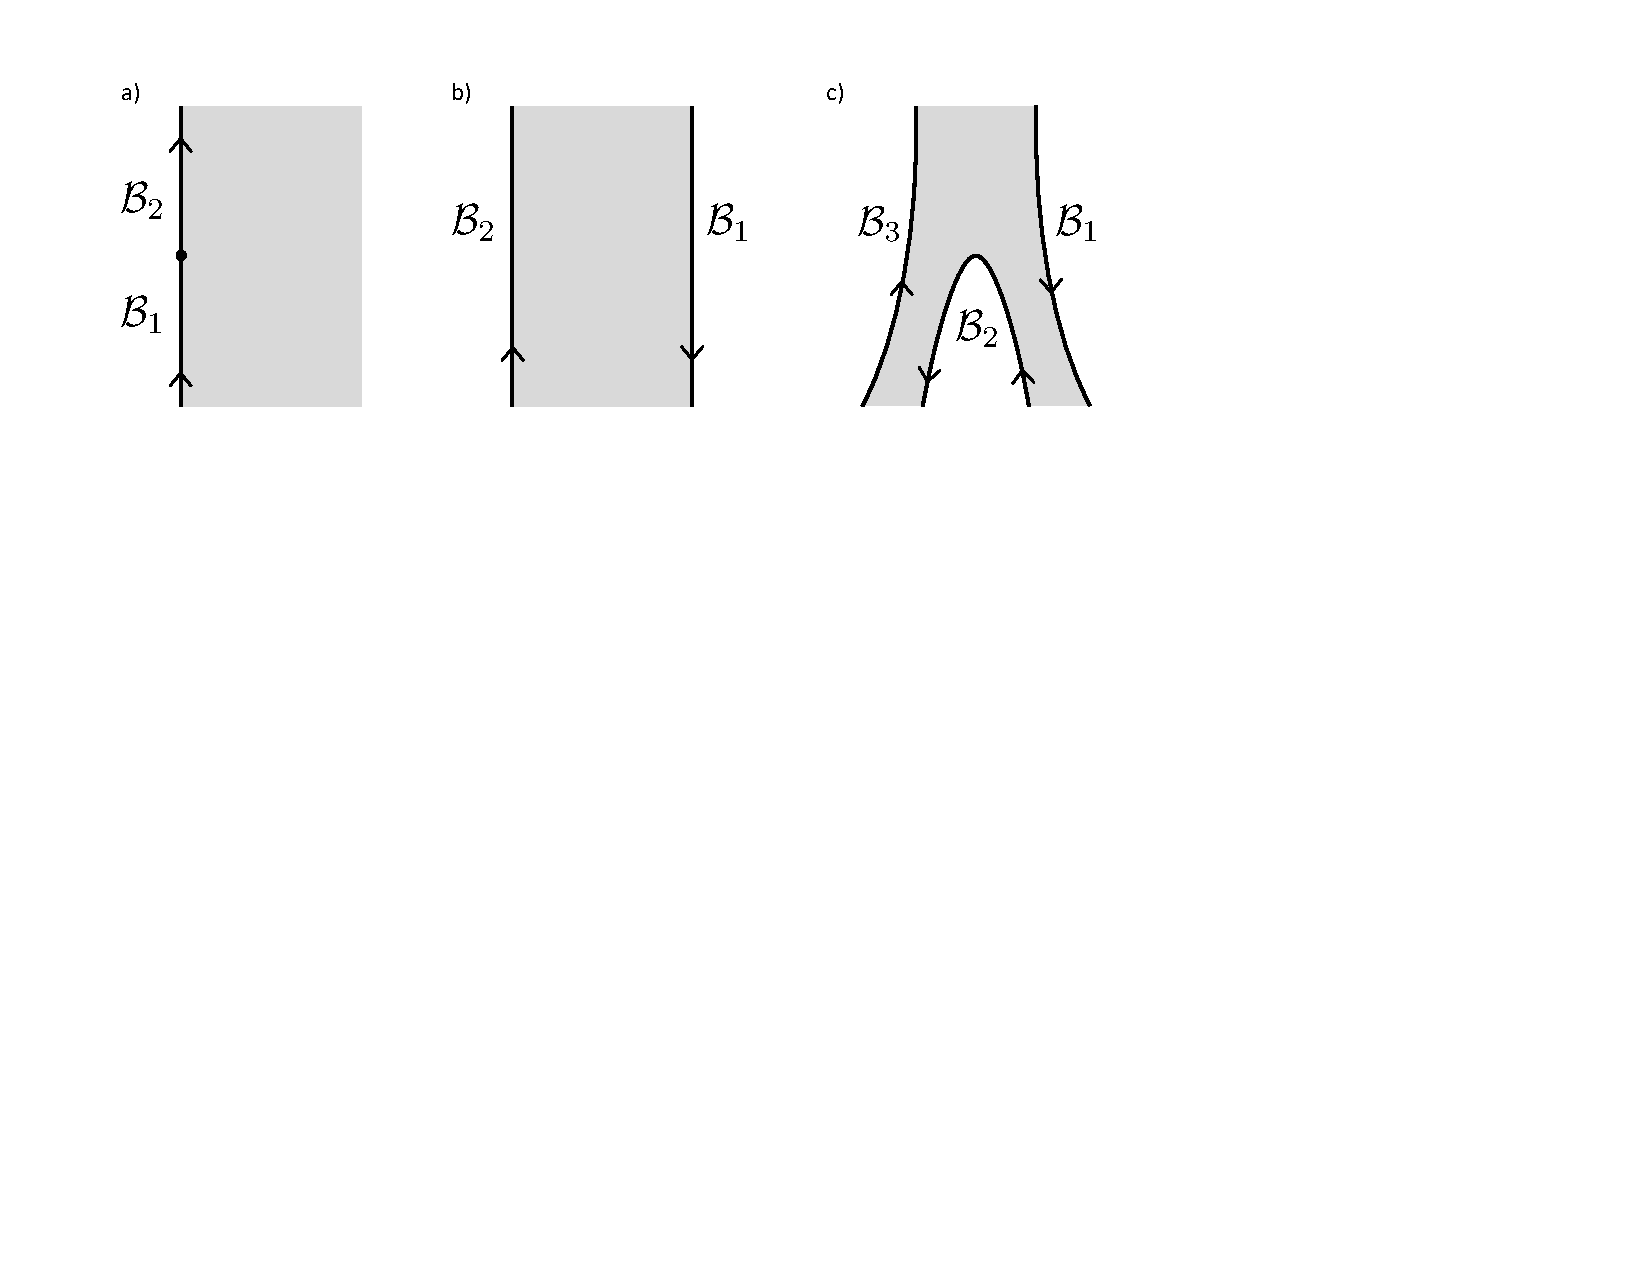
\includegraphics[width=0.86\textwidth]{figures/1_Conventions.pdf}
 \caption{\small (a) 对于二维流形 $\Sigma$ 的左边界，约定“时间”沿箭头方向向上流动，因此 $\B_1$ 在下、$\B_2$ 在上的边界条件衔接表示从 $\B_1$ 到 $\B_2$ 的跃迁，代数上即 $\Hom(\B_1,\B_2)$ 的元素。(b) 通过共形变换可把它映成条带，$\B_2$ 在左、$\B_1$ 在右；图中表示 $\Hom(\B_1,\B_2)$ 的元素从图底部传播到顶部。换一个看法，从顶到底读同一幅图，表示对偶空间 $\Hom(\B_2,\B_1)$ 的元素向下传播。（两种看法可通过平面旋转 $\pi$ 互换，旋转保持定向并交换 $\B_1$ 与 $\B_2$；反射会反转平面定向，不允许。）向上与向下的箭头表示 $\Hom(\B_1,\B_2)$ 对 $\B_2$ 协变、对 $\B_1$ 反变。(c) 态射的自然合成 $\Hom(\B_2,\B_3)\otimes\Hom(\B_1,\B_2)\to\Hom(\B_1,\B_3)$（其中 $\B_1$ 映到 $\B_2$，再映到 $\B_3$）对应此图。}
 \label{explained}
\end{figure}

一般地，若 $\B_1$ 是 $A$-膜，则 $A$-模型中 $(\B_1,\B_1)$ 弦的物理态空间是结合代数 $\A$。若 $\B_2$ 是另一 $A$-膜，则 $(\B_1,\B_2)$ 或 $(\B_2,\B_1)$ 物理态的类似空间是 $\A$-模（确切地说，是右 $\A$-模与左 $\A$-模）。$A$-模型与量子化的联系，来自把这一想法用于 $\B_1=\B_\cc$、$\B_2$ 为拉格朗日膜的情形。为简便，我们沿用数学术语，把 $A$-模型中（任意 $\B_1,\B_2$ 的）$(\B_1,\B_2)$ 物理态空间记作 $\Hom(\B_1,\B_2)$。基本想法是：把 $(\B_1,\B_2)$ 弦与 $(\B_2,\B_3)$ 弦接合成 $(\B_1,\B_3)$ 弦，可描述为态射的合成 $\Hom(\B_2,\B_3)\otimes\Hom(\B_1,\B_2)\to\Hom(\B_1,\B_3)$，其中 $\B_1$ 先映到 $\B_2$，再映到 $\B_3$。一般地，$\Hom(\B_1,\B_2)$ 对 $\B_2$ 协变、对 $\B_1$ 反变。与此相关，若 $\B_1$ 的支撑为 $T_1$、$\CP$ 丛为 $E_1$，$\B_2$ 的支撑为 $T_2$、$\CP$ 丛为 $E_2$，则非常粗略地说，$\Hom(\B_1,\B_2)$ 是 $T_1\cap T_2$ 上取值 $E_1^\vee\otimes E_2$ 的某种截面空间（$E_1^\vee$ 是 $E_1$ 的对偶）。示意地，
\be\label{kogo}\Hom(\B_1,\B_2)\sim \Gamma(T_1\cap T_2, E_1^\vee\otimes E_2).\ee
这是非常示意性的说法，因为我们没有说明允许哪类截面（这依赖于所考虑的膜类型的细节），而且一般而言完整的故事要复杂得多。式 \eqref{kogo} 的要点只在于强调 $E_1$ 取了对偶而 $E_2$ 没有。弦与态射关系的一些约定见图 \ref{explained}。

至少在 $\hbar$ 很小时，加法地有：$\Hom(\B_\cc,\B_\cc)$ 是 $Y$ 的上同调群之直和，
\be\label{poklo}\Hom(\B_\cc,\B_\cc)=\oplus_{r=0}^{\dim_\C Y}H^r(Y,\O),\ee
其中 $\O$ 是 $Y$ 上的平凡复线丛。整数 $r$ 标记上同调类的费米子数或“鬼数”。此结果的推导在附录 \ref{details} 中概述，仿照 \cite{GW} 第 2.2 节。由于弦态相接合（或相乘）时费米子数可加，$r=0$ 的态自身构成一个环。上同调的这一部分因而特别重要。许多有趣例子中 $r>0$ 的上同调实际上消失。

当 $Y$ 是仿射代数簇（由 $\C^N$ 上某些多项式函数的零点定义）时，环 $\Hom(\B_\cc,\B_\cc)$ 特别有意思，我们继续在此情形下讨论。仿射簇的层上同调在 $r>0$ 时消失，故只需考虑 $r=0$ 上同调，它作为向量空间是 $Y$ 上的全纯函数空间。如第 \ref{amo} 节所解释，只考虑关于坐标的多项式函数。在普通乘法下，$Y$ 上的全纯函数构成交换结合环 $\A_0$。但这不是 $\A=\Hom(\B_\cc,\B_\cc)$ 的环结构。相反，如 \cite{KW} 第 11.1 节在若干先前发展 \cite{KO,BrS,Ka,Pe,Gu,AZ} 之后所证明的，也如下文将解释的，$\A$ 是 $\A_0$ 的结合非交换形变。

\subsubsection{与形变量子化的关系}\label{defrel}

此推导的基本想法如下。一般地，$A$-模型由某个底层超对称 $\sigma$-模型构造：选取一个满足 $Q^2=0$ 的超荷 $Q$，并限制到 $Q$-不变的可观测量。由于 $Q^2=0$，$Q$-不变可观测量不受作用量中 $Q$-恰当项 $\{Q,\cdots\}$ 的影响。在二维流形 $\Sigma$ 上，考虑靶为 $Y$ 的 $\sigma$-模型及其映射 $X:\Sigma\to Y$。设 $\omega_\C=\omega-\i\sB$ 为 $A$-模型的复化辛形式。若 $\Sigma$ 无边界，作用量取简单形式
\be\label{simpform}\sI=\int_\Sigma X^*(\omega_\C)+\int_\Sigma\{Q,\cdots\}.\ee
换言之，除 $\omega_\C$ 的拉回外，一切都是 $Q$-恰当的。在我们的设定中 $\omega_\C=-\i\Omega$。因此例如 $\Sigma$ 是以 $S^1$ 为边界的圆盘 $D$ 时，作用量为
\be\label{toldo}\sI=-\i\int_DX^*(\Omega)+\int_D\{Q,\cdots\}.\ee
欧氏号差下 Feynman 积分的被积函数为 $\exp(-\sI)$，故该积分示意地是
\be\label{oldo}\int\D X\cdots\exp\left(\i\int_D\Omega\right)\exp\left(-\int_D\{Q,\cdots\}\right).\ee
（这里 $\D X\cdots$ 指对 $X$ 及其它场的积分。）更一般地，可在圆盘边界上插入算符。这类算符表示 $(\B_\cc,\B_\cc)$ 弦，故对应 $Y$ 上的全纯函数 $f_1,\cdots,f_k$（或后文讨论的高次上同调类）。如第 \ref{uses} 节，在圆盘边界上取点 $r_1,r_2,\cdots,r_k$，并记 $f_i(r_i)=f_i(X(r_i))$。于是，边界标以 $\B_\cc$、带边界算符插入的圆盘上 $A$-模型计算的 Feynman 积分为
\be\label{noldo}\int\D X\cdots\exp\left(\i\int_D\Omega\right)\exp\left(-\int_D\{Q,\cdots\}\right)f_1(r_1)f_2(r_2)\cdots f_k(r_k).\ee

这个积分与 $Y$ 上全纯函数环 $\A_0$ 的形变量子化有关。先描述这个概念。形式上，复流形 $Y$ 上全纯函数环的形变量子化，与第 \ref{uses} 节简述的实辛（或 Poisson）流形的形变量子化相当类似，只是被形变的是全纯函数环。若 $\Omega=\frac12\sum_{i,j}\Omega_{ij}\d y^i\d y^j$（$y^i$ 为 $Y$ 的局部全纯坐标），$\Omega^{ij}$ 为 $\Omega_{ij}$ 的逆矩阵，则全纯函数的 Poisson 括号按通常方式定义为
\be\label{pb}\{f,g\}=\sum_{i,j}\Omega^{ij}\partial_i f\,\partial_j g.\ee
于是在形变环 $\A$ 中，对应全纯函数 $f,g$ 的代数元素 $\h f,\h g$ 满足
\be\label{hb}\h f\h g-\h g\h f=-\i\hbar\h{\{f,g\}}_0+\O(\hbar^2),\ee
其中通过写 $\Omega=\frac{1}{\hbar}\Omega_0$（$\Omega_0$ 固定）引入了形变参数，$\{~,~\}_0$ 是用 $\Omega_0$ 定义的 Poisson 括号。在 $\h f\h g$ 按 $\hbar$ 的展开中，$\hbar^n$ 阶项应是形如 $\partial^k f\partial^{2n-k}g$ 的项之和。

积分 \eqref{noldo} 与形变量子化的关系，最精确的解释见 \cite{W}。首先回忆第 \ref{uses} 节：实辛流形 $M$ 的形变量子化可由对映射 $x:S^1\to M$ 的空间 $\pP$ 的积分描述：
\be\label{pyccl}\bigl\langle f_1f_2\cdots f_k\bigr\rangle=\int_\pP\D x\,\exp\left(\i\int_Dx^*(\omega)\right)f_1(r_1)f_2(r_2)\cdots f_k(r_k).\ee
这里假定 $x:S^1\to M$ 接近常值，并把它的像收缩为 $M$ 中一点，从而延拓为 $x:D\to M$（$D$ 是以 $S^1$ 为边界的圆盘）。$M$ 以 $Y$ 为复化，$\omega=\omega_J$ 解析延拓为 $\Omega$。$\pP$ 的复化是映射 $X:S^1\to Y$ 的空间 $\h\pP$。在形变量子化中，可假定 $X:S^1\to Y$ 接近常值，同样得到同伦意义下的延拓 $X:D\to Y$。函数 $\exp(\i\int_Dx^*(\omega))$ 解析延拓为 $\h\pP$ 上的全纯函数，即 $\exp(\i\int_DX^*(\Omega))$。注意正是这个函数作为因子出现在式 \eqref{oldo} 中，作用量的其余部分是 $Q$-恰当的。$M$ 上适当的光滑函数 $f_1,f_2,\cdots,f_k$ 可解析延拓为 $Y$ 上的全纯函数，仍记作 $f_1,f_2,\cdots,f_k$。形式上，式 \eqref{pyccl} 中的表达式 $\D x\exp(\i\int_Dx^*(\omega))$（$\D x$ 为 Feynman 路径积分测度）是无穷维流形 $\pP$ 上的最高次微分形式。它解析延拓为 $\h\pP$ 上的最高次全纯形式 $\D X\exp(\i\int_DX^*(\Omega))$。要在复流形（这里是无穷维流形 $\h\pP$）上积分最高次全纯形式，需要一个中间维的积分圈。因此例如，若 $\Gamma$ 是 $\h\pP$ 中适当类型的中间维圈，我们或可望使积分
\be\label{pyclo}\int_\Gamma\D X\exp\left(\i\int_DX^*(\Omega)\right)f_1(r_1)f_2(r_2)\cdots f_k(r_k)\ee
有意义。

$\h\pP$ 中中间维圈的一个例子是原来的 $\pP$，即映入 $M\subset Y$ 的映射。取此 $\Gamma$ 时，积分 \eqref{pyclo} 化回 \eqref{pyccl}，给出了理解形变量子化的框架。\cite{W} 所证明的是：边界为 $\B_\cc$、边界上带算符插入的圆盘上的积分 \eqref{noldo}，可解释为取另一个积分圈的积分 \eqref{pyclo}，该圈\footnote{我们马上会讨论，需要作一个修正，因为这个圈并不完全是中间维的。}由那些可延拓为关于复结构 $K$ 全纯的映射 $X:D\to Y$ 的映射 $X:S^1\to Y$ 组成。在使积分 \eqref{pyclo} 有意义的“几乎中间维”圈类中，$\Gamma$ 的选取不影响把该积分与 $Y$ 的形变量子化相联系的论证。此陈述的一个有限维类比是：若 $Z$ 是带最高次全纯形式 $\Omega$ 的复流形，则周期积分 $\int_\Gamma\Omega$ 所满足的微分方程不依赖于圈 $\Gamma\subset Z$ 的选取。

这个简短总结省略了很多，但还有一个细节需要解释，尽管它在本文中没有直接作用。如关于式 \eqref{cycl} 的讨论所解释的，若能使积分 \eqref{pyclo} 有意义，就会得到形变 $\A_0$ 的结合代数 $\A$，以及 $\A$ 上的一个迹。迹是复值线性函数 $\h f\to\la\h f\ra$，满足 $\la\h f\h g\ra=\la\h g\h f\ra$。对光滑流形 $M$，迹的经典极限是与辛测度的积分：$f\to\int_M\frac{\omega^n}{n!}f$，其中 $n=\frac12\dim M$。对带全纯函数 $f$ 的复辛流形 $Y$，这没有如此直接的类比。$\frac{\omega^n}{n!}f$ 最接近的类比是 $\frac{\Omega^n}{n!}f$，它是最高次全纯微分形式；但无法在 $Y$ 上积分 $\frac{\Omega^n}{n!}f$。若使用限制到 $M$ 的积分圈 $\pP$，这没有困难；但若使用与 $\B_\cc$ 相联系的积分圈，就需修改其中一个算符的定义，结果得不到迹。我们主要关心非紧 $Y$，因为若 $Y$ 紧，就没有非常值全纯函数可供量子化。若 $Y$ 非紧，对偶是普通 $\bar\partial$ 上同调与紧支撑 $\bar\partial$ 上同调之间的配对。若 $f_1,\cdots,f_{k-1}$ 是 $Y$ 上的全纯函数，则应取 $f_k\in H^{\dim_\C Y}_{\mathrm{cpct}}(Y,\O)$，即最高次紧支撑 $\bar\partial$ 上同调类。于是式 \eqref{pyclo} 中积分的经典极限是 $\int_Yf_1f_2\cdots f_k\frac{\Omega^n}{n!}$。这是良定义的积分，量子修正也良定义。由式 \eqref{pyclo} 的关联函数，按式 \eqref{woppo} 的算符乘积展开，可构造结合代数 $\A$，它在 $\hbar\to0$ 时约化为全纯函数的交换代数 $\A_0$。但这个代数没有附带迹，因为把其中一个算符取为紧支撑上同调类破坏了循环对称。

\cite{W} 对此点的解释是：由指标定理，与 $\B_\cc$ 相联系的圈 $\Gamma$ 实际上比中间维高 $2n=\dim_\C Y$，故不很适合全纯形式的积分。补偿办法是把其中一个函数 $f_i$ 换成 $(0,2n)$-形式。

\subsubsection{实际形变}\label{actual}

对一般的 $Y$，这个构造给出的是 $\hbar$ 的形式幂级数环上的形变量子化。这对 $A$-模型用于量子化还不够；为此需要能把 $\hbar$ 当作复数。等价地，需要取 $\Omega$ 为 $Y$ 上确定的全纯辛形式。此时我们说 $A$-模型给出了一个\textbf{实际}形变代数 $\A$，而不只是形式形变。如第 \ref{amo} 节所述，其充分条件是：以 $Y$ 为靶的底层量子 $\sigma$-模型（$A$-模型是它的扭转版本）应作为完整的量子场论真正存在。特别地，若 $Y$ 容许完备超 Kähler 度量，则确实如此。

在讨论全纯函数环形变量子化的同一问题时，Kontsevich \cite{K2} 提出：粗略地说，若 $Y$ 可通过添加无穷远除子紧化、且 $\Omega$ 在该除子上有极点，则实际形变存在。Kontsevich 的判据有些类似于如下条件：Tian--Yau 关于完备 Calabi--Yau 度量的定理 \cite{TY} 的超 Kähler 版本会预言 $Y$ 具有完备超 Kähler 度量。（这样的定理似乎只在复维 2 可用，那里 Calabi--Yau 度量自动是超 Kähler 的。）

在 \cite{KW,GW} 讨论的一些重要情形中，可直接证明（无需了解量子 $\sigma$-模型）$\sigma$-模型微扰论在有限步后终止，因此 $A$-模型给出实际形变。这发生在 $Y$ 具有伸缩对称、或至少具有渐近伸缩对称、且 $\hbar$ 按正次数缩放时。

例如，考虑复簇 $x^2+y^2+z^2=\j^2$（式 \eqref{osuc}）。此流形在无穷远处渐近于锥 $x^2+y^2+z^2=0$。它有渐近伸缩对称 $(x,y,z)\to\lambda(x,y,z)$，其中 $\j$ 按次数 1 缩放。取全纯辛形式 $\Omega=\d x\d y/(z\hbar)$，其中 $\hbar$ 也按次数 1 缩放。伸缩对称意味着，在得知可以令 $\hbar=1$ 之后，令 $\hbar=1$ 不会损失任何东西。经典环 $\A_0$ 由 $x,y,z$ 生成，次数均为 1，交换关系如 $xy=yx$，另有附加关系 $x^2+y^2+z^2=\j^2$。形变环在 $x,y,z,\j,\hbar$ 的联合缩放下不变，并有明显的旋转 $x,y,z$ 的 $\SO(3)$ 对称性。综合这些事实可得 \cite{GW}：形变环由 $\h x\h y-\h y\h x=\hbar\h z$ 及其循环置换，以及 $\h x^2+\h y^2+\h z^2=\j^2-\frac14\hbar^2$ 给出，其中只有最后一项的数值系数 $\frac14$ 需要一些分析。这个例子也说明了另两个判据：空间 $Y$ 容许完备超 Kähler 度量（Eguchi--Hanson 度量），并有具备 Kontsevich 所需性质的紧化（即 $\bCP^3$ 中的二次曲面 $x^2+y^2+z^2=w^2$）。类似地可考虑由更高次多项式定义的仿射簇。对复辛流形 $x^n+y^n+z^n=b$（$b$ 为复常数），辛形式为 $\d x\d y/z^{n-1}$，可以发现 $n=3$ 时两个判据都满足，$n>3$ 时都不满足。

复余切丛将在第 \ref{cotangent} 节详细讨论，它们有精确的伸缩对称，因而是具有实际形变的例子，尽管一般认为它们不容许完备超 Kähler 度量。它们确实满足 Kontsevich 的判据。

\subsection{拉格朗日 $A$-膜与量子化}\label{abq}

\subsubsection{Hilbert 空间的定义}\label{hilbdef}

现在引入一个拉格朗日 $A$-膜，并解释它与量子化的关系。我们沿用 \cite{GW} 第 2.3 节的说明。一些重要的示意性例子此前已由 \cite{AZ} 分析过。

要量子化实辛流形 $M$，选取支撑为 $M$、带某个 $\CP$ 丛的秩 1 拉格朗日 $A$-膜 $\B$。秩 1 拉格朗日 $A$-膜的特征是其 $\CP$ 丛的曲率 $\sF$ 满足 $\sF+\sB=0$。由于已取 $\sB=\omega_J$，曲率必须是 $\sF=-\omega_J$。如第 \ref{amo} 节所述，我们的目标是用辛结构 $\omega_J$ 量子化 $M$。回忆几何量子化的第一步是引入曲率等于辛形式（此处为 $\omega_J$）的预量子线丛 $\frL$。由于 $\sF$ 是 $\frL$ 曲率的负值，可以把 $\B$ 的 $\CP$ 丛解释为 $\frL^{-1}$。这个等同合理的一个迹象是反常匹配：几何量子化中松散地称为预量子线丛的东西，更准确地说是 $\spinc$ 结构（第 \ref{gq} 节讨论过）；类似地，秩 1 膜的 $\CP$ 丛其实也是 $\spinc$ 结构而非复线丛，如脚注 \ref{anomdesc} 所述。

于是，带预量子线丛 $\frL$ 的 $M$ 的膜量子化的 Hilbert 空间定义为
\[
\H=\Hom(\B,\B_\cc),
\]
即 $(\B,\B_\cc)$ 系统的物理态空间。对偶空间是 $\H'=\Hom(\B_\cc,\B)$。把 $\H$ 而非 $\H'$ 认作 Hilbert 空间，是因为 $\A=\Hom(\B_\cc,\B_\cc)$ 从左边作用在 $\H=\Hom(\B,\B_\cc)$ 上，而从右边作用在 $\H'=\Hom(\B_\cc,\B)$ 上。若可能，人们总倾向于用环的左作用，因此如上定义 $\H$ 是自然的。把 $\H$ 称为 Hilbert 空间而不只是向量空间，是指 $\H$ 有自然的 Hermite 内积；这将在第 \ref{hermitian} 节描述。

为理解这个量子 Hilbert 空间定义的动机，我们构造开弦低能态的有效作用量，该弦的左、右边界分别落在 $\B_\cc$ 与 $\B$ 上。设弦的世界面为 $\R\times I$，$\R$ 以 $\tau$ 参数化，$I$ 为区间。$I$ 两端的边界条件使得没有费米零模；此陈述的解释见附录 \ref{details}。玻色零模沿 $I$ 为常数，故描述映射 $X:\R\to M$，可用函数 $x^i(\tau)$ 表示，$x^i$ 为 $M$ 的局部坐标。$x^i(\tau)$ 的有效作用量是什么？体作用量给出若干关于 $\d x^i/\d\tau$ 二次的项，但最相关的项关于 $\d x^i/\d\tau$ 线性，来自弦两端与 $\CP$ 丛的边界耦合。回顾式 \eqref{kogo}，在 $\Hom(\B,\B_\cc)$ 的定义中，弦的一端是 $\B_\cc$ 的 $\CP$ 丛，另一端是 $\B$ 的 $\CP$ 丛的对偶（即逆）。$\B_\cc$ 的 $\CP$ 丛完全平凡，$\B$ 的 $\CP$ 丛为 $\frL^{-1}$，其对偶为预量子线丛 $\frL$。若 $\sA$ 是 $\frL$ 上的联络，则弦端点与 $\frL$ 的耦合对低能有效作用量的贡献就是
\be\label{kixx}\sI=\int_\R x^*(\sA).\ee
这正是第 \ref{uses} 节引入的作用量，那里预量子线丛上的联络记作 $\sT/\hbar$。如那里所解释的，形式上这是与量子化相联系的作用量。

如第 \ref{uses} 节所讨论的，作用量 \eqref{iff} 或 \eqref{kixx} 没有更多信息其实无法量子化。正确的说法不是 $\Hom(\B,\B_\cc)$ 的 $A$-模型计算归结为作用量 \eqref{kixx} 的量子化；而是：$A$-模型（对适当的 $Y$）良定义而式 \eqref{kixx} 的量子化有歧义，这意味着在约化到 \eqref{kixx} 时丢失了一些信息。结论的正确表述是：$\H=\Hom(\B,\B_\cc)$ 就是 $A$-模型给出的、带预量子线丛 $\frL$ 的 $M$ 的量子化答案。

\subsubsection{若干问题}\label{ques}

说 $A$-模型给出了 $M$ 量子化的这个答案，会引出若干问题。以下是一些明显的问题：

(1) $A$-模型的物理态空间通常不是 Hilbert 空间。它通常没有任何类型的内积（甚至不定内积也没有）。在目前语境中，$A$-模型如何产生 Hermite 内积？

(2) 作用在量子 Hilbert 空间 $\H$ 上的可观测量是什么？

(3) 当标准量子化方法可用时，这个概念与它们相容吗？

第一个问题将在第 \ref{hermitian} 节回答。

关于第二个问题，$A$-模型直接给出的答案是：$\A=\Hom(\B_\cc,\B_\cc)$ 作用在 $\H=\Hom(\B,\B_\cc)$ 上。若 $M$ 是实仿射簇、$Y$ 是其复化，这个答案最令人满意。此时如第 \ref{abranes} 节所述，$\A$ 是 $Y$ 上多项式函数环 $\A_0$ 的结合非交换形变。$Y$ 上的多项式函数环与 $M$ 上的多项式函数环相同（$M$ 上的多项式函数可解析延拓为 $Y$ 上的多项式函数；$Y$ 上的非零多项式限制到 $M$ 上非零）。所以被量子化的 $M$ 上函数是多项式函数。这是相当令人满意的答案。例如若 $M=\R^{2n}$，被量子化的函数就是坐标与动量的多项式。在第 \ref{hermitian} 节我们将看到，$\A$ 中对应 $\H$ 上 Hermite 算符的元素正是 $\tau$-不变元。

然而，用膜量子化辛流形 $M$ 对实仿射簇之外的许多例子也有意义。在许多其它情形中 $\A_0$ 小得多，于是得不到如此丰富的、可量子化为 $\H$ 上算符的 $M$ 上函数。此时一般而言，什么是有趣的可观测量就不那么明显了。不过还有另一种定义作用在 $\H$ 上算符的办法，即与拉格朗日对应相联系的算符。这将在第 \ref{symq} 节解释。例如，在与几何 Langlands 相关、将在别处研究的情形 \cite{GaW} 中，$\A_0$ “很小”，$\A$ 实际上是交换的且同构于 $\A_0$。在那个特例中，重要的是考虑与拉格朗日对应相联系的算符（确切地说是 Hecke 对应，物理上与 't Hooft 算符相联系）。

最后一个问题——把膜量子化与标准量子化方法作比较——是第 \ref{comparing} 节的主题。

\subsubsection{推广}\label{genera}

到目前为止，我们考虑的拉格朗日膜的支撑为 $M$，即反全纯对合 $\tau:Y\to Y$ 的不动点集的一个分支。如第 \ref{hermitian} 节将讨论的，这个条件对在空间 $\H$ 上定义 Hermite 内积很重要。但其它类型的拉格朗日膜也重要。

由于把 $Y$ 视为辛结构为 $\omega_K$ 的辛流形，按定义，说 $L$ 是拉格朗日子流形意味着 $\omega_K$ 限制到 $L$ 上为零。但 $\omega_J$ 限制到 $L$ 上没有一般性约束。若该限制也为零，则 $L$ 实际上是关于 $Y$ 的复辛结构 $\Omega_I=\omega_J+\i\omega_K$ 的拉格朗日子流形。这样的 $L$ 是 $Y$ 的复子流形\footnote{若 $\omega_J$ 与 $\omega_K$ 限制到 $L$ 上均为零，这意味着沿 $L$，它们都是 $L$ 的切丛与法丛之间的配对。由此可知 $I=\omega_K^{-1}\omega_J$ 把 $L$ 的切丛映到自身，故 $L$ 是复子流形。}，所以它其实是复拉格朗日子流形。由于对任何 $A$-膜 $\B$，$\Hom(\B,\B_\cc)$ 都是 $\A=\Hom(\B_\cc,\B_\cc)$ 的模，特别地当 $\B$ 是支撑在复辛流形 $L$ 上的拉格朗日膜时也是如此。这类膜是 $(B,A,A)$ 型的：它们关于复结构 $I$ 是 $B$-膜（因为 $L$ 是复子流形，而 $\B$ 的 $\CP$ 丛平坦，故关于 $I$ 全纯），关于辛结构 $\omega_J$ 与 $\omega_K$ 是 $A$-膜（因为 $L$ 关于这两个结构都是拉格朗日的，且其 $\CP$ 丛平坦）。与 $(B,A,A)$ 型膜相联系的模很有意思，并将在第 \ref{comparing} 节成为重要工具，但它们与 $L$ 的量子化没有密切关系。确实，由于 $\omega_J$ 与 $\omega_K$ 限制到 $L$ 上都为零，上述讨论没有在 $L$ 上给出辛结构，故我们没有量子化 $L$ 的自然问题。（若 $Y$ 是超 Kähler 的，它还有第三个辛结构 $\omega_I$，而复拉格朗日子流形 $L$ 关于 $\omega_I$ 是辛的。但我们研究的 $A$-模型以及膜 $\B_\cc$、$\B$ 对 $\omega_I$ 不敏感。）

与 $L$ 的量子化相关的是相反情形：$\omega_J$ 限制到 $L$ 上非退化。若 $\B$ 是支撑在任一这样的 $L$ 上的秩 1 $A$-膜，则 $\Hom(\B,\B_\cc)$ 具有人们期待的、关于辛结构 $\omega=\omega_J|_L$ 的 $L$ 的量子化的大部分性质。构造中只有一步失败，即 Hermite 内积的定义。如第 \ref{hermitian} 节将解释的，这个内积的定义要求 $L$ 是 $Y$ 的某个反全纯对合的不动点集。直观上应当如此：若 $L$ 不是 $Y$ 的反全纯对称的不动点集，则 $Y$ 上的全纯函数限制到 $L$ 上何时为实并不自然，于是没有明显办法判定 $Y$ 上哪些全纯函数应在 $L$ 的量子化中成为 Hermite 算符。因此应当不能在 $\Hom(\B,\B_\cc)$ 上定义 Hermite 内积。

在 \cite{GW} 第 3.7 节中描述了 $\SL(2,\C)$ 的余伴随轨道（即式 \eqref{cosu} 定义的仿射簇 $Y$）的拉格朗日子流形 $L$ 的例子，使 $\omega_J$ 限制到 $L$ 上非退化，但 $L$ 不是 $Y$ 的任何反全纯对合的不动点集。这样的 $L$ 例如与 $\SL(2,\R)$ 或其 Lie 代数的各种有趣但非酉的表示相联系。

另一个推广是考虑 $\B$ 为支撑在 $M$（或更一般的拉格朗日子流形 $L$）上、秩 $m>1$ 的拉格朗日膜。讨论此情形时，为简单起见假定 $M$ 是 spin 流形，从而不必讨论通常涉及 spin 的反常。于是 $M$ 的 $\CP$ 丛是秩 $m$ 的平坦向量丛 $\U\to M$，结构群为 $\UU(m)$。在此情形下，$\Hom(\B,\B_\cc)$ 将是量子化概念的一种秩 $m$ 推广。这种量子化推广的存在或许稍令人惊讶。不过不难看出，在几何量子化可用的情形中这样的推广确实存在。例如设 $M=T^*N$。则按几何量子化的精神，可考虑由 $\K^{1/2}\otimes\U\to N$ 的 $\ltwo$ 截面构成的 Hilbert 空间。或者设 $M$ 有 Kähler 极化，则可考虑 Hilbert 空间 $H^0(M,K^{1/2}\otimes\U)$。

\subsection{Hermite 内积}\label{hermitian}

本节沿用 \cite{GW} 第 2.4 节，讨论在 $A$-模型中定义 Hermite 内积需要什么。其实拓扑 $A$-模型与 $B$-模型两种情形可以平行处理，且 $B$-模型情形也有意思。因此我们把两种情形放在一起考虑：考虑由酉超对称二维 $\sigma$-模型扭转得到的任意二维拓扑场论。扭转为选取满足 $Q^2=0$ 的超荷的线性组合 $Q$，并将其视为微分。

这种拓扑场论中通常的内积是双线性形式（对每个变量线性），而不是 Hermite 或半双线性形式（对一个变量线性、对另一个反线性）。因此若 $\B_1,\B_2$ 是两个膜，则 $\Hom(\B_1,\B_2)$ 与 $\Hom(\B_2,\B_1)$ 之间总有非退化双线性配对，可由圆盘上的两点函数计算。所以，求 $\Hom(\B_1,\B_2)$ 与自身的半双线性配对，等价于求从 $\Hom(\B_1,\B_2)$ 到 $\Hom(\B_2,\B_1)$ 的反线性映射。

底层 $\sigma$-模型总有反线性对称，即我们称为 $\Theta$ 的 $\CPT$ 对称。它反转弦的定向，故把 $\Hom(\B_1,\B_2)$ 映到 $\Hom(\B_2,\B_1)$。然而 $\Theta$ 不能完成我们想要的事，因为它不是用给定 $Q$ 定义的拓扑场论的对称。这样的 $Q$ 从不是 Hermite 的（因 $Q^2=0$），而 $\Theta$ 把 $Q$ 共轭为 $Q^\dagger$。换言之，$\Theta$ 把微分为 $Q$ 的 $A$-或 $B$-模型映到微分为 $Q^\dagger$ 的共轭 $A$-或 $B$-模型。

要找到与给定 $Q$ 相联系的拓扑场论的反线性对称，需把 $\Theta$ 与 $\sigma$-模型的线性对称 $\tau$ 复合，后者把 $Q^\dagger$ 共轭回 $Q$。这样的对称在 $A$-模型或 $B$-模型中都可以存在。在 $A$-模型中，$\tau$ 应反转用于定义 $A$-模型的辛形式 $\omega$ 的符号。\footnote{反转辛结构符号的实辛流形微分同胚称为“反辛的”，这是仿照“反全纯”一词——后者描述反转复结构符号的微分同胚——的用法。}在 $B$-模型中，$\tau$ 应反转用于定义 $B$-模型的复结构 $J$ 的符号。换言之，$A$-模型中需要 $\tau^*(\omega)=-\omega$，$B$-模型中需要 $\tau^*(J)=-J$。于是 $\Theta_\tau=\tau\Theta$ 将是从 $A$-模型或 $B$-模型到自身的反线性映射。

更一般地，有 $B$-场时，$\Theta$ 把复化辛形式为 $\omega_\C=\omega-\i\sB$ 的 $A$-模型映到以 $-\bar\omega_\C$ 代替 $\omega_\C$ 的共轭 $A$-模型。为补偿这一点，$\tau$ 在反转 $\omega$ 符号的同时应满足 $\tau^*(\sB)=\sB$。

为得到最好的性质，$\tau$ 应是自伴的、满足 $\tau^2=1$，并与 $\Theta$ 交换。我们假定这些条件，它们蕴含 $\Theta_\tau^2=1$ 且 $\Theta_\tau$ 自伴。

一般地，$\tau$ 把膜 $\B_1,\B_2$ 映到另一些膜 $\bar\B_1,\bar\B_2$，于是 $\Theta_\tau$ 把 $\Hom(\B_1,\B_2)$ 映到 $\Hom(\bar\B_2,\bar\B_1)$。因此 $\Theta_\tau$ 与 $A$-或 $B$-模型的自然双线性配对 $(\,,\,)$ 复合，给出 $\Hom(\B_1,\B_2)$ 与 $\Hom(\bar\B_1,\bar\B_2)$ 之间的半双线性配对，定义为
\be\label{wofo}\langle\psi,\psi'\rangle=(\Theta_\tau\psi,\psi').\ee
要得到 $\Hom(\B_1,\B_2)$ 与自身的半双线性配对，需要 $\bar\B_1=\B_1$、$\bar\B_2=\B_2$；换言之，所考虑的膜必须是 $\tau$-不变的。此时可以问该半双线性形式是否为 Hermite 的，即 $\overline{\langle\psi,\psi'\rangle}=\langle\psi',\psi\rangle$。这个条件确实满足，因为 $(\,,\,)$ 对称而 $\Theta_\tau$ 自伴且反线性。

对 $\tau$-不变的膜 $\B_1,\B_2$，我们来给出算符 $\O:\Hom(\B_1,\B_2)\to\Hom(\B_1,\B_2)$ 的伴随的一般描述。首先，一般有对偶或转置算符 $\O^*$，从对偶空间 $\Hom(\B_2,\B_1)$ 到自身。$\O^*$ 由如下条件刻画：对 $\psi\in\Hom(\B_1,\B_2)$、$\chi\in\Hom(\B_2,\B_1)$，
\be\label{chardual}(\O^*\chi,\psi)=(\chi,\O\psi).\ee
另一方面，对 $\psi,\psi'\in\Hom(\B_1,\B_2)$，伴随算符 $\O^\dagger$ 应满足
\be\label{addual}\la\O^\dagger\psi',\psi\ra=\la\psi',\O\psi\ra.\ee
把这些条件与 $\la~,~\ra$ 的定义结合，得 $(\Theta_\tau\O^\dagger\psi',\psi)=(\Theta_\tau\psi',\O\psi)=(\O^*\Theta_\tau\psi',\psi)$。故 $\Theta_\tau\O^\dagger=\O^*\Theta_\tau$；又因 $\Theta_\tau^2=1$，有
\be\label{adjform}\O^\dagger=\Theta_\tau\O^*\Theta_\tau.\ee

我们来考察 $Y$ 为实辛流形 $M$ 的复化时 Hermite 内积的这一构造。此时如第 \ref{amo} 节所述，$M$ 是反全纯对合 $\tau:Y\to Y$ 的不动点集。因此支撑在 $M$ 上的拉格朗日膜 $\B$ 是 $\tau$-不变的。由于我们考虑 $\omega=\omega_K$、$\sB=\omega_J$ 的 $A$-模型，希望 $\omega_K$ 在 $\tau$ 下为奇（以满足 $\tau^*(\omega)=-\omega$），$\omega_J$ 为偶（使 $\sB$ 为 $\tau$-不变\footnote{或者可作 $B$-场规范变换令 $\sB=0$，并给 $\B_\cc$ 以 $\CP$ 曲率 $\omega_J$。此时为使 $\B_\cc$ 为 $\tau$-不变，需要 $\tau^*(\omega_J)=\omega_J$。}）。这些条件由式 \eqref{tabush} 满足。膜 $\B_\cc$ 是 $\tau$-不变的，因为其 $\CP$ 丛平凡。于是我们确实得到 $\H=\Hom(\B,\B_\cc)$ 上的 Hermite 结构。同样的构造给出对偶空间 $\H'=\Hom(\B_\cc,\B)$ 上的 Hermite 结构；这两个结构在反线性同构 $\Theta_\tau:\H\cong\H'$ 下等价。

由于 $\A=\Hom(\B_\cc,\B_\cc)$ 线性作用于 $\H$，现在可以问 $\A$ 中哪些元素 $x$ 对应 $\H$ 上的 Hermite 算符。按上述 Hermite 结构的定义，答案是：$x$ 对应 Hermite 算符当且仅当它与 $\Theta_\tau$ 交换。由于 $\Theta_\tau$ 反线性且 $\Theta_\tau^2=1$，每个 $x$ 可写成 $x=x_1+\i x_2$，其中 $x_1,x_2$ 与 $\Theta_\tau$ 交换，并在量子化后成为 Hermite 的。

一般地，对 $\tau$-不变的膜 $\B_1,\B_2$，我们在 $\Hom(\B_1,\B_2)$ 上定义的 Hermite 形式不是正定的。它总是非退化的，因为 $\Theta_\tau$ 是同构，而 $A$-或 $B$-模型的双线性配对 $(\,,\,)$ 非退化。

在更具体的量子化语境中，能说的最好是：充分接近经典极限时，这个 Hermite 形式是正定的。例如在 Kähler 极化的情形，辛形式的周期足够大时便充分接近经典极限；在余切丛的量子化中，总预期正定性成立。

\subsection{光滑函数与分布}\label{smooth}

作为本导引的结尾，我们勾勒一种展示 $\H=\Hom(\B,\B_\cc)$ 元素的有用办法。更多细节将在第 \ref{comparing} 节给出。主要构件是另一个 $A$-膜 $\F$。实践中一般取 $\F$ 为支撑在某个拉格朗日子流形 $L\subset Y$ 上的秩 1 膜。$L$ 通常\textbf{不}与我们正在研究其量子化的相空间 $M$ 重合。取元素 $\alpha\in\Hom(\F,\B_\cc)$、$\beta\in\Hom(\B,\F)$，把它们复合得 $\psi=\alpha\circ\beta\in\Hom(\B,\B_\cc)$，如图 \ref{outline}(a) 所示。类似地，若 $\F'$ 是又一个 $A$-膜，也配有 $\alpha'\in\Hom(\F',\B_\cc)$、$\beta'\in\Hom(\B,\F')$，则可复合得 $\psi'=\alpha'\circ\beta'\in\Hom(\B,\B_\cc)$。按第 \ref{hermitian} 节定义的内积 $\la\psi',\psi\ra$ 可由矩形上的路径积分计算，见图 \ref{outline}(b)。

\begin{figure}[htbp]
 \centering
 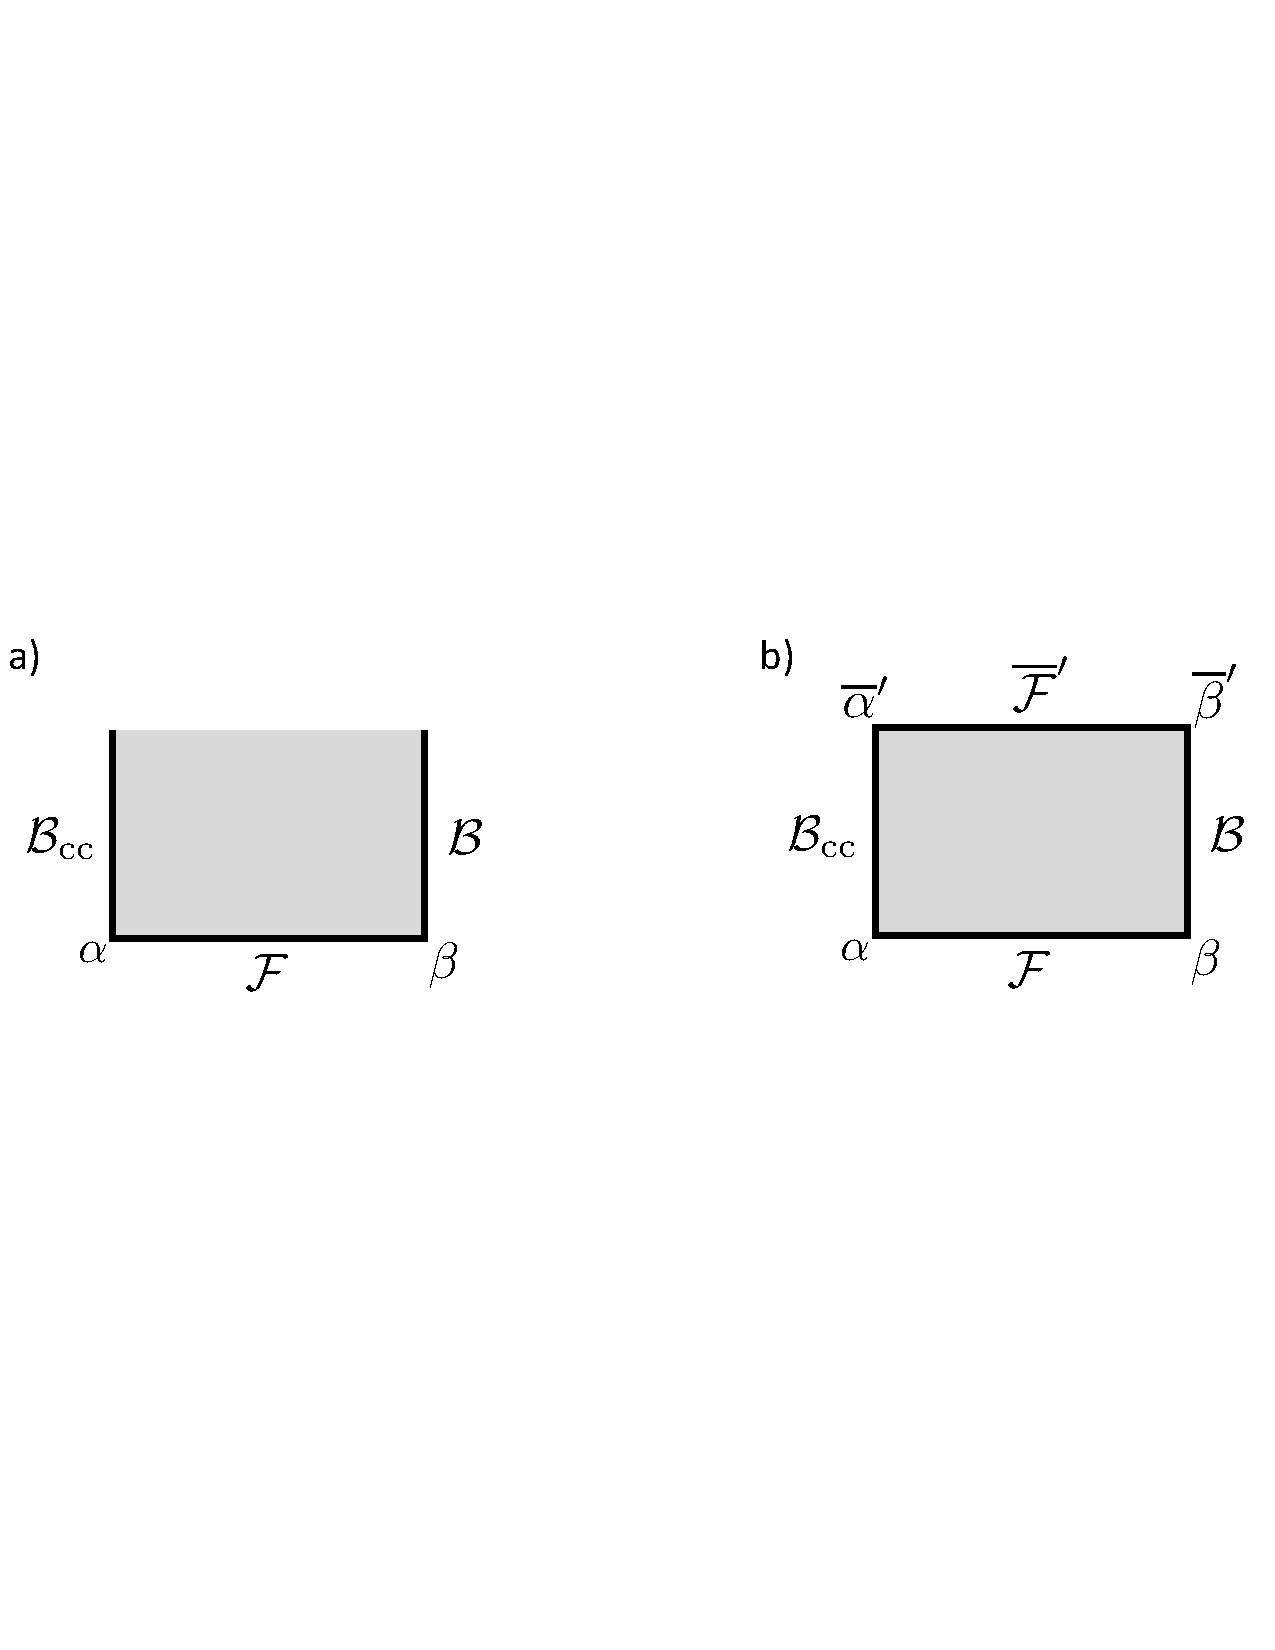
\includegraphics[width=0.72\textwidth]{figures/NewBrane.pdf}
 \caption{\small (a) 一个辅助膜 $\F$ 连同某些附加数据，可用来构造 $\Hom(\B,\B_\cc)$ 中的一个态。一般地这是分布态。(b) 用膜 $\F,\F'$ 构造的态之间的内积，可由矩形上的路径积分计算，$\F$ 在底部，$\bar\F'$（$\F'$ 的 $\tau$-共轭）在顶部。}
 \label{outline}
\end{figure}

然而应当问：$\psi$ 与 $\psi'$ 是哪一类态？这里我们想到的是分析中的问题，例如在普通空间 $\R^3$ 中运动的粒子的量子力学里不同类波函数之间的区别。$\R^3$ 上粒子量子力学的舞台通常理解为 $\ltwo$ 函数构成的 Hilbert 空间。但在一个有良好动机的物理问题中，粒子的波函数通常比这好得多：是无穷远处快速衰减的光滑函数。数学上，这样的函数构成所谓的 Schwartz 空间。另一方面，发展量子力学时也方便考虑不可归一化的态，例如在点 $\vec x_0\in\R^3$ 处有 delta 函数支撑的波函数 $\delta^3(\vec x-\vec x_0)$，或在动量空间有 delta 函数支撑的平面波 $\exp(\i\vec p\cdot\vec x)$。数学上这些不可归一化的态称为分布；按定义，分布与 Schwartz 空间中任意向量都有良定义的内积。

若相空间 $M$ 紧，则 Hilbert 空间 $\H$ 有限维，不会出现这类分析问题。但若 $M$ 非紧，就应问刚才勾勒的构造产生哪类波函数。一个简单的观察是：若 $\F$ 或 $\F'$ 有紧支撑，则可期望图 \ref{outline}(b) 中矩形对应的振幅良定义且收敛。若 $\F$ 与 $\F'$ 都没有紧支撑，一般这个振幅可能不良定义。这引出如下尝试性解释：完全一般的 $A$-膜 $\F$ 在此构造中产生不可归一化的分布态；而有紧支撑的 $A$-膜 $\F$ 产生 Schwartz 空间中向量的类比——这种向量可与任意分布配对。

\section{比较膜量子化与几何量子化}\label{comparing}

\subsection{复余切丛与形变量子化}\label{cotangent}

几何量子化与膜量子化，是为量子化辛流形 $M$ 引入必要额外结构的两种不同方式。这两大量子化方法在什么情况下一致？我们能期望的最好答案，是找到 $M$ 的复化 $Y$ 与 $M$ 的极化 $\P$ 上的条件，使得基于 $Y$ 的膜量子化等价于基于 $\P$ 的几何量子化。本节将针对第 \ref{gq} 节引入的两类基本极化——$M$ 的实极化与复极化——解释这样的等价判据。

先描述人们可能期望比较膜量子化与几何量子化的最明显情形。设 $M=T^*N$ 是余切丛，带自然辛结构 $\omega=\sum_i\d p_i\d q^i$，其中 $q^i$ 为 $N$ 的局部坐标，$p_i$ 为余切丛纤维上的线性函数。再设 $W$ 是第 \ref{amo} 节意义下 $N$ 的复化。则 $Y=T^*W$ 是 $M$ 的复化。$Y$ 的自然全纯辛形式仍可写成 $\Omega=\sum_i\d p_i\d q^i$（此时 $q^i$ 与 $p_i$ 是 $W$ 上及 $T^*W\to W$ 纤维上的局部全纯坐标），它是 $\omega$ 的解析延拓。若 $Y$ 的 $A$-模型存在，就可用它量子化 $M$，并把结果与利用 $M=T^*N$ 的余切丛描述所作的几何量子化比较。

先讨论 $Y$ 的形变量子化，即讨论 $\Hom(\B_\cc,\B_\cc)$。余切丛有极大约束力的伸缩对称。为利用此对称，方便的是稍作推广，取 $\Omega=\sum_i\d p_i\d q^i/\hbar$（在得知可以令 $\hbar=1$ 后即可令之）。有一个伸缩对称使 $q^i$ 不变，而 $p_j$ 与 $\hbar$ 的次数为 1。

这个伸缩对称是 $\C^*$ 在这些变量上的作用。我们将假定形变量子化应以 $\C^*$-不变的方式施行。若 $\C^*$ 的某个 $\UU(1)$ 子群是底层 $\sigma$-模型的对称（所关心的 $A$-模型由该 $\sigma$-模型导出），则确乎如此。（在将别处讨论的几何 Langlands 应用中这是对的 \cite{GaW}。）全纯性会把这样的 $\UU(1)$ 对称提升为 $\C^*$。若没有底层 $\UU(1)$ 对称，经由 $\B_\cc$ 的形变量子化可能不是 $\C^*$-不变的。

例如设 $W=\C^n$、$Y=\C^{2n}$，使坐标 $q^i,p_j$ 可整体定义。Poisson 括号为 $\{p_i,q^j\}=\delta_i^j$、$\{q^i,q^j\}=\{p_i,p_j\}=0$。要求量子换位子与 Poisson 括号在 $\hbar^2$ 阶修正以内一致，并施加伸缩对称，则量子换位子最一般的形式是
\begin{align}\label{genform}
[\h p_i,\h q^j]&=\i\hbar\delta^j_i\cr
[\h p_i,\h p_j]&=\hbar^2f_{ij}(\h q^k)\cr
[\h q^i,\h q^j]&=0.\end{align}
Jacobi 恒等式 $[\h p_i,[\h p_j,\h p_k]]+\cdots=0$ 蕴含 $\partial_if_{jk}+\partial_jf_{ki}+\partial_kf_{ij}=0$，故存在函数 $g_k$ 使 $f_{ij}=\partial_ig_j-\partial_jg_i$。于是把 $\h p_i$ 换成 $\h p_i'=\h p_i-\i\hbar g_i(q^k)$（此代换与伸缩关系相容），可把式 \eqref{genform} 化为
\begin{align}\label{genformtwo}
[\h p_i',\h q^j]&=\i\hbar\delta^j_i\cr
[\h p_i',\h p_j']&=0\cr
[\h q^i,\h q^j]&=0.\end{align}
因此，$p_i$ 与 $q^j$ 的多项式函数（如第 \ref{abranes} 节所述，这是我们唯一允许的函数）的量子形变代数，就是把 $q^j$ 表示为乘算符、$p_i$ 表示为 $-\i\hbar\frac{\partial}{\partial q^i}$ 所得的代数。当然，最后这个公式在初等量子力学中很熟悉。有了对 $\h q^i$ 与 $\h p_j$ 的这一刻画，结合代数 $\Hom(\B_\cc,\B_\cc)$ 可刻画为 $\C^n$ 上多项式全纯微分算符的代数。在建立这个与微分算符的关系时，重要的是只允许对 $p$ 的依赖为多项式的函数；下文将始终施加此条件。类似地也只允许对 $q$ 的多项式依赖。于是 $\h p$ 与 $\h q$ 的函数对应多项式全纯微分算符。

现在考虑更一般的 $W$。局部上可化归前一情形：用 $W$ 的开集 $\U\subset W$（选得使 $\U$ 同构于 $\C^n$ 中一个区域）代替 $W$，用 $T^*\U$ 代替 $Y$。把靶空间 $Y=T^*W$ 换成开集（此处为 $T^*\U$），在 $\sigma$-模型中一般不是好操作。不过，由于 $\sigma$-模型微扰论涉及靶空间中常值映射附近的小涨落，限制到开集在 $\sigma$-模型微扰论中没有问题。通常这只能给出微扰信息，但我们处在不寻常的情形：这已经足够，因为伸缩对称意味着到 $\hbar^2$ 阶的微扰论给出全部答案。我们选择形如 $T^*\U$ 的开集，是因为这样的集合在伸缩下不变，从而伸缩论证适用。因此可以把 $\Hom(\B_\cc,\B_\cc)$ 视为 $W$ 上的层：对任何开集 $\U\subset W$，联系以 $T^*\U$ 上的 $\Hom(\B_\cc,\B_\cc)$。应当承认，尽管这一步在数学上说得通且显得很自然，它在物理上是否完全自然并不清楚。最好能为这一步找到更自然的物理解释，或在后续论证中设法避开它。

若取 $\U$ 小到同构于 $\C^n$ 中的开球，事情就简单了。一旦限制到这样的 $\U$ 对应的 $T^*\U$，坐标 $q_i,p^j$ 可整体定义，并可像前面那样提升为表示 $(\B_\cc,\B_\cc)$ 弦的算符。故上述分析适用于任何这样的集合。

现在用小开集 $\U_\alpha$ 覆盖 $W$，每个同构于 $\C^n$ 中的开集，且交集拓扑平凡。于是 $Y$ 被开集 $T^*\U_\alpha$ 覆盖。对每个 $\alpha$，取 $\U_\alpha$ 的局部坐标 $q^i_\alpha$ 及余切丛的纤维坐标 $p_{j,\alpha}$。在交集 $T^*(\U_\alpha\cap\U_\beta)$ 中，坐标之间的关系为
\begin{align}\label{relco}
q^i_\alpha&=h^i_{\alpha\beta}(q^k_\beta)\cr
p_{i,\alpha}&=M_{\alpha\beta}(q)^k_i\,p_{k,\beta},\end{align}
其中 $h^i_{\alpha\beta}$ 是某些全纯函数，$M_{\alpha\beta}{}^i_j$ 是 $\partial_ih^j_{\alpha\beta}$ 的逆矩阵。

量子层面，伸缩对称不允许 $q$ 的转移公式有任何改变，故必须有 $\h q^i_\beta=h^i_{\alpha\beta}(\h q^k)$，其中 $q$ 的函数与之前相同。但对 $p$，伸缩对称允许 $\hbar$ 阶修正，于是公式变为 $\h p_{i,\alpha}=M_{\alpha\beta}(\h q)^k_i\h p_{k,\beta}+\i\hbar r_{i,\alpha\beta}(\h q)$，其中 $r_{i,\alpha\beta}$ 为某些全纯函数。然而为满足 $[\h p_{i,\alpha},\h p_{j,\beta}]=0$，需要 $\partial_ir_{j,\alpha\beta}-\partial_jr_{i,\alpha\beta}=0$，因此（由于 $\U_\alpha\cap\U_\beta$ 拓扑平凡）存在全纯函数 $w_{\alpha\beta}$ 使 $r_{j,\alpha\beta}=\partial_jw_{\alpha\beta}(\h q)$。于是 $\h p$ 的变换为
\be\label{transp}\h p_{i,\alpha}=M_{\alpha\beta}(\h q)^k_i\h p_{k,\beta}+\i\hbar\partial_iw_{\alpha\beta}(\h q).\ee
若在区域 $\U_\alpha\cap\U_\beta$ 中只用一组坐标 $q^i$（而不用两组坐标 $q^i_\alpha,q^i_\beta$），此公式会简单得多。此时矩阵 $M$ 换成 1，公式简化为
\be\label{transpo}\h p_{i,\alpha}=\h p_{i,\beta}+\i\hbar\partial_iw_{\alpha\beta}.\ee
这就分离出了 $\h p$ 变换中的非经典部分。

立即可得 $w_{\alpha\beta}=-w_{\beta\alpha}$；三重交上的相容性告诉我们 $\partial_k(w_{\alpha\beta}+w_{\beta\gamma}+w_{\gamma\alpha})=0$，故 $\phi_{\alpha\beta\gamma}=w_{\alpha\beta}+w_{\beta\gamma}+w_{\gamma\alpha}$ 是复常数。在四重交上，这些常数自动满足
\be\label{cocrel}\phi_{\alpha\beta\gamma}-\phi_{\beta\gamma\delta}+\phi_{\gamma\delta\alpha}-\phi_{\delta\alpha\beta}=0,\ee
因而定义出 $H^2(W,\C)$ 的一个元素 $[\phi]$。

若 $[\phi]$ 实际取值于 $2\pi\i\cdot H^2(W,\Z)$，即（在可能把 $w_{\alpha\beta}$ 平移常数之后）每个 $\phi_{\alpha\beta\gamma}$ 都是 $2\pi\i$ 的整数倍，则量 $S_{\alpha\beta}=\exp(w_{\alpha\beta})$ 满足 $S_{\alpha\beta}S_{\beta\gamma}S_{\gamma\alpha}=1$，可视为复线丛 $\L\to W$ 的转移函数。具体地说，$\L$ 如下：在每个 $\U_\alpha$ 中，$\L$ 的截面就是函数 $\psi_\alpha$；但不同开集 $\U_\alpha$ 与 $\U_\beta$ 中的函数由 $\psi_\alpha=S_{\alpha\beta}\psi_\beta$ 相联系。在此情形，上述公式可解释为：$q$ 与 $p$ 的函数的量子化给出作用在 $\L$ 截面上的全纯微分算符。换言之，设 $D_\alpha$ 与 $D_\beta$ 分别是作用在相应开集 $\U_\alpha$ 与 $\U_\beta$ 中函数上的全纯微分算符。为把它们解释为 $W$ 上整体定义的全纯微分算符限制到这些区域，需要 $D_\alpha(S_{\alpha\beta}\psi)=S_{\alpha\beta}D_\beta\psi$，即 $D_\alpha=S_{\alpha\beta}D_\beta S^{-1}_{\alpha\beta}$。特别地，在区域 $\beta$ 中为 $\h p_i=-\i\hbar\frac{\partial}{\partial q^i}$ 的算符，在区域 $\alpha$ 中将是 $\h p_i+\i\hbar\partial_i\log S_{\alpha\beta}=\h p_i+\i\hbar\partial_iw_{\alpha\beta}$，与式 \eqref{transp} 相符。

这有如下推广。\footnote{\label{zany}我们将描述的情形出现在量子化的重要例子中，但并不完全一般。例如，若 $W$ 紧，且 $[\phi]$ 的 Hodge 分解含有 $(2,0)$ 型部分，则下文所述不适用。}设 $\L\to W$ 是全纯线丛，并设在各开集 $\U_\alpha$ 中取定 $\L$ 的平凡化后，$\L$ 可由 $\U_\alpha\cap\U_\beta$ 中的转移函数 $e^{x_{\alpha\beta}}$ 描述。设 $w_{\alpha\beta}=\lambda x_{\alpha\beta}$，$\lambda$ 为某复数。若 $\lambda$ 为整数，则函数 $e^{w_{\alpha\beta}}=e^{\lambda x_{\alpha\beta}}$ 是某个全纯线丛的转移函数，即 $\L^\lambda$。此时上一段的讨论适用，$q$ 与 $p$ 的函数的量子化是作用在 $\L^\lambda$ 截面上的全纯微分算符。对一般的复 $\lambda$，线丛 $\L^\lambda$ 并不存在，但这只是因为三重交 $\U_\alpha\cap\U_\beta\cap\U_\gamma$ 中转移函数之积 $e^{\lambda(x_{\alpha\beta}+x_{\beta\gamma}+x_{\gamma\alpha})}$ 是 $c$-数而不等于 1。由于微分算符与 $c$-数交换，无论 $\L^\lambda$ 是否作为线丛存在，作用在 $\L^\lambda$ 上的微分算符这个概念都有意义。于是 $q$ 与 $p$ 的量子化函数自然地理解为作用在 $\L^\lambda$ 上的微分算符。

更一般地，设 $\L_i\to W$ 是全纯线丛，由全纯函数 $x_{i,\alpha\beta}$ 给出的转移函数 $e^{x_{i,\alpha\beta}}$ 描述。若 $w_{\alpha\beta}=\sum_i\lambda_ix_{i,\alpha\beta}$，其中 $\lambda_i$ 为某些整数，则 $\otimes_i\L_i^{\lambda_i}$ 作为线丛有意义，$p$ 与 $q$ 的量子化函数是作用在 $\otimes_i\L_i^{\lambda_i}$ 上的微分算符。若 $w_{\alpha\beta}=\sum_i\lambda_ix_{i,\alpha\beta}$ 而 $\lambda_i$ 为更一般的复系数，则 $\otimes_i\L_i^{\lambda_i}$ 作为线丛没有意义，但作用在 $\otimes_i\L_i^{\lambda_i}$ 上的微分算符仍有意义，且 $p$ 与 $q$ 的量子化函数自然地是作用在 $\otimes_i\L_i^{\lambda_i}$ 上的全纯微分算符。

我们将松散地把 $\otimes_i\L_i^{\lambda_i}$ 称为线丛的复幂（尽管更准确地说，是这种复幂的张量积）。我们所描述的情形对量子化很重要，但如脚注 \ref{zany} 所述，它不是最一般的可能性。

一个重要细节是：若 $\RR$ 是容许平坦联络的全纯线丛，则作用在 $\otimes_i\L_i^{\lambda_i}$ 上的全纯微分算符与作用在 $\RR\otimes_i\L_i^{\lambda_i}$ 上的全纯微分算符相同。这是因为平坦线丛可由其 $c$-数整体和乐刻画；而微分算符与 $c$-数交换，故全纯微分算符对 $\otimes_i\L_i^{\lambda_i}$ 与 $\RR\otimes_i\L_i^{\lambda_i}$ 之别不敏感。

结果表明，在 $Y=T^*W$ 的情形，$\Hom(\B_\cc,\B_\cc)$ 就是作用在线丛复幂上的微分算符层。证明这一点的一个快捷办法是方便地选取 $A$-膜 $\B_0$，并利用 $\Hom(\B_\cc,\B_\cc)$ 可作用在 $\Hom(\B_0,\B_\cc)$ 上这一事实。为此我们将利用 $(B,A,A)$ 型拉格朗日膜。

\begin{yizhu}[线丛的“复幂”是什么意思]
$\L=\otimes_i\L_i^{\lambda_i}$ 在 $\lambda_i$ 非整数时并非真正的线丛：局部转移函数 $e^{\lambda_i x_{\alpha\beta}}$ 仍是 $U(1)$-值的，但三重交不再自动满足上闭链条件，故整体可能“粘不起来”。原文仍使用它，是因为全纯微分算符与这些 $c$-数因子交换，所以“作用在 $\L$ 的截面上”这句话在局部仍有确切含义；在 $W$ 紧且 $[\phi]$ 含 $(2,0)$ 部分时，原文脚注已提醒这一描述会失效。[来源：I 级]
\end{yizhu}

\subsection{$(B,A,A)$ 型膜作为工具}\label{lagbr}

$(B,A,A)$ 型膜是关于复结构 $I$ 的 $B$-膜，又是关于 $\omega_J$ 与 $\omega_K$ 的 $A$-膜。它们在第 \ref{genera} 节引入。我们特别关心秩 1 的 $(B,A,A)$ 型拉格朗日膜。这样膜的支撑是复拉格朗日子流形 $L$。我们已取 $B$-场为 $\sB=\omega_J$，它限制到复拉格朗日子流形 $L$ 上为零。因此支撑在 $L$ 上的秩 1 $A$-膜 $\B_0$ 的 $\CP$ 曲率条件 $\sF+\sB=0$ 化为 $\sF=0$。故这样膜的 $\CP$ 丛是平坦 $\spinc$ 结构。如第 \ref{genera} 节所述，若 $\B_0$ 是这样的膜，则 $\Hom(\B_0,\B_\cc)$ 是 $Y$ 上函数量子形变代数的模，尽管这个模不能自然地解释为 $L$ 的量子化。

我们可以用这样的模作为理解 $\Hom(\B_\cc,\B_\cc)$ 的工具。作为探针，考虑一个方便的 $(B,A,A)$ 型膜，即支撑在余切丛零截面 $W\subset T^*W$ 上的膜。我们假定 $W$ 容许平坦 $\spinc$ 结构 $\L$，因而是一个秩 1 拉格朗日膜 $\B_0$ 的支撑。由于考虑的是沿 $W$ 局部的论证，$\L$ 是否整体存在其实不重要；同样，稍后我们会看到 $\L$ 的选取也无关紧要。

余切丛的零截面在纤维伸缩下不变。故 $\Hom(\B_0,\B_\cc)$ 可在 $\hbar$ 很小时计算。考虑到 $\B_\cc$ 的 $\CP$ 丛平凡，按附录 \ref{details} 的一般分析，结果是 $\Hom(\B_0,\B_\cc)\cong\oplus_{q=0}^{\dim_\C W}H^q(W,K_W^{1/2}\otimes\L^{-1})$。特别地，只取 $q=0$，$\Hom(\B_\cc,\B_\cc)$ 必须能作用在 $H^0(W,K_W^{1/2}\otimes\L^{-1})$ 上，即 $K_W^{1/2}\otimes\L^{-1}$ 的全纯截面空间。由于 $\L^{-1}$ 平坦，它在此不起作用：作用在 $K_W^{1/2}\otimes\L^{-1}$ 截面上的全纯微分算符，与作用在 $K_W^{1/2}$ 截面上的全纯微分算符相同。因此 $\Hom(\B_\cc,\B_\cc)$ 必须是作用在 $K_W^{1/2}$ 截面上（而不是某个其它线丛上）的微分算符层。

按先前解释，作用在 $K_W^{1/2}$ 上的微分算符无论 $K_W^{1/2}$ 是否整体作为线丛存在都有意义。不过或许值得说明：类似地，若 $K_W^{1/2}$ 确实作为线丛存在，它的选取也无关紧要。$K_W^{1/2}$ 的不同选取相差一个满足 $\RR^2$ 平凡的线丛 $\RR$ 的张量积。这样的 $\RR$ 容许平坦联络，故张量以 $\RR$ 对作用在 $K_W^{1/2}$ 上的全纯微分算符没有影响。

在附录 \ref{opposite} 中，我们解释另一种（数学上更标准的）办法，说明在余切丛情形 $\Hom(\B_\cc,\B_\cc)$ 是作用在 $K_W^{1/2}$ 截面上的微分算符层，而不是线丛的某个其它复幂。

\subsection{复余切丛与量子化}\label{ccb}

现在回到实辛流形 $M=T^*N$，问 $Y=T^*W$（$W$ 为 $M$ 的复化）的 $A$-模型如何用来研究 $M$ 的量子化。

我们将利用另一个 $(B,A,A)$ 型拉格朗日膜 $\cF$。在进入细节前，先说明策略（第 \ref{smooth} 节已简述）。我们将描述相当自然的元素 $\alpha\in\Hom(\B_\cc,\cF)$ 与 $\beta\in\Hom(\cF,\B)$，其中 $\B_\cc$ 仍为典范余各向同性 $A$-膜，$\B$ 为支撑在 $M$ 上的秩 1 拉格朗日 $A$-膜。一旦定义了 $\alpha$ 与 $\beta$，就容易用三元组 $\cF,\alpha,\beta$ 定义 $\H'=\Hom(\B_\cc,\B)$ 中的元素 $\psi'$，而 $\H'$ 是 Hilbert 空间 $\H=\Hom(\B,\B_\cc)$ 的对偶。（第 \ref{hermitian} 节定义的自然反线性映射 $\Theta_\tau$ 给出 $\H$ 与 $\H'$ 的同构，但在不引用它时，我们区分 $\H$ 与 $\H'$。）其实，对我们将要选取的 $\cF$，$\psi'$ 将是分布波函数。这与第 \ref{smooth} 节的讨论一致，因为 $\cF$ 没有紧支撑。

代数上，把 $\alpha\in\Hom(\B_\cc,\cF)$ 与 $\beta\in\Hom(\cF,\B)$ 复合，得 $\psi'=\beta\circ\alpha\in\H'=\Hom(\B_\cc,\B)$。用图来说，就是考虑图 \ref{strip} 中的条带，$\B_\cc$ 在左、$\cF$ 在上、$\B$ 在右，角上为 $\alpha,\beta$。受此类图启发，我们把 $\alpha,\beta$ 这样的对象称为\textbf{角}。\footnote{在二维中，把这些对象称为“角”似乎缺乏动机，因为这些角可通过共形映射拉直。这个术语的动机来自二维以上的类似构造：在那里这种表示两种不同边界条件衔接的角不能被共形拉直。关于某些四维超对称理论中此类衔接的系统研究见 \cite{GR}。这样的四维构造可通过黎曼面上的紧化约化到二维，这与几何 Langlands 有关。}条带上的路径积分自然产生向量 $\psi'\in\H'=\Hom(\B_\cc,\B)$。确实，若提供态 $\psi\in\Hom(\B,\B_\cc)$ 作为条带底部的边界条件，则条带上的路径积分只产生一个数。与图 \ref{strip} 类似但 $\F$ 在底部的图产生 $\H$ 中的向量，这已在第 \ref{smooth} 节解释。

\begin{figure}[htbp]
 \centering
 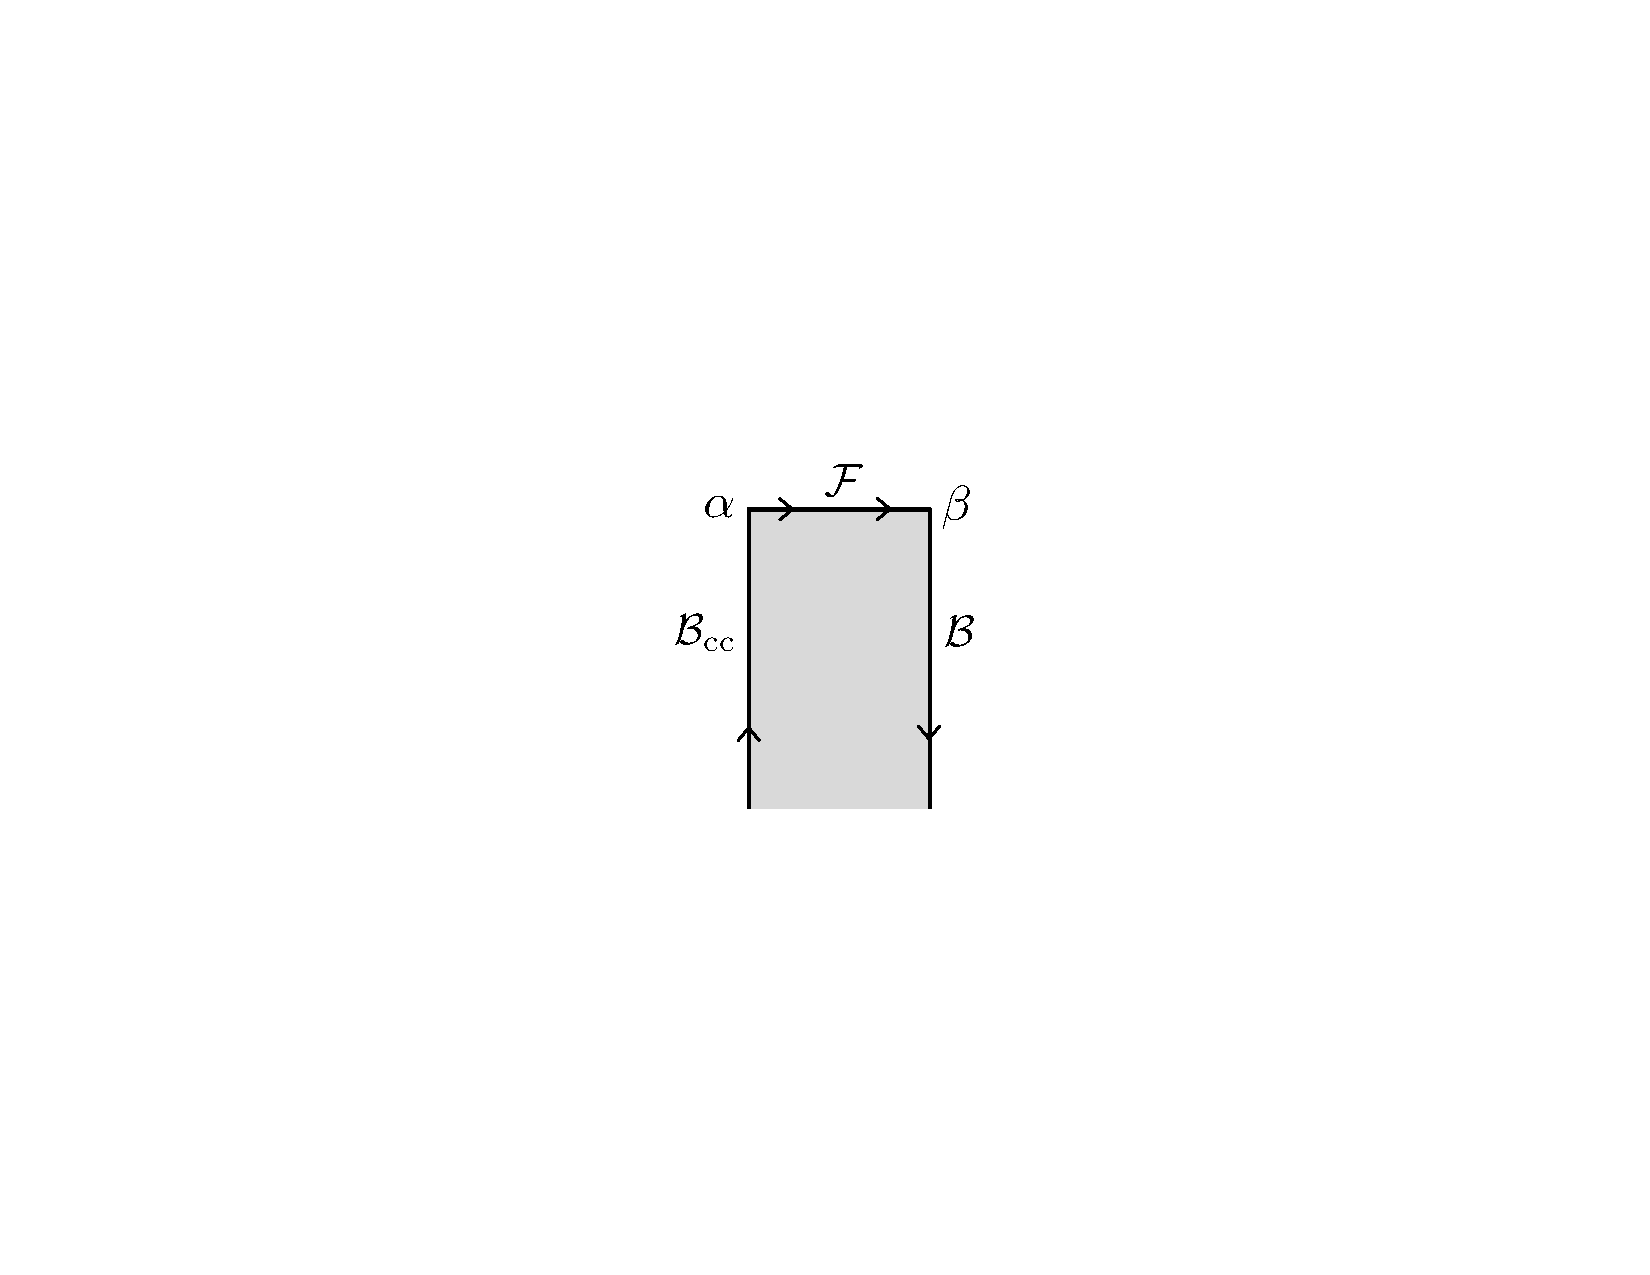
\includegraphics[width=0.36\textwidth]{figures/2_Strip.pdf}
 \caption{\small 条带，$\B_\cc$ 在左、$\F$ 在上、$\B$ 在右，角上为适当的 $\alpha,\beta$。按图 \ref{explained}(a) 的约定，$\alpha$ 表示 $\Hom(\B_\cc,\F)$ 的元素，$\beta$ 表示 $\Hom(\F,\B)$ 的元素；它们的合成是 $\H'=\Hom(\B_\cc,\B)$ 的元素。图中该元素从条带顶部（它在此产生）向下传播。}
 \label{strip}
\end{figure}

对 $\cF$，取支撑在余切丛 $T^*W$ 的纤维 $F$ 上的膜，$F$ 是包含某点 $w\in W$ 的纤维。最终将专门取 $w\in N$，但暂时允许任意 $w$。把 $w$ 邻域中 $W$ 的局部坐标记作 $q^i$，把余切丛纤维上的共轭函数记作 $p_i$。

由于 $F\cong\C^n$ 有唯一 spin 结构，$\cF$ 的 $\CP$ 丛就是平坦线丛；又因 $F$ 单连通，这个平坦线丛平凡。$F$ 在余切丛伸缩下不变（虽非逐点不变），故 $\cF$ 也在此伸缩下不变。于是如第 \ref{lagbr} 节，$\Hom(\B_\cc,\cF)$ 可在 $\hbar\to0$ 极限下计算。仍由附录 \ref{details}，结果为 $\Hom(\B_\cc,\cF)=H^0(F,K_F^{1/2})$，这里用了 $F\cong\C^n$ 时高阶上同调消失。此外 $K_F^{1/2}$ 平凡，故 $H^0(F,K_F^{1/2})$ 等同于 $F$ 上的全纯函数空间。由于不允许在无穷远指数增长的波函数，$H^0(F,K_F^{1/2})$ 可等同于参数化 $F$ 的坐标 $p_i$ 的多项式函数空间。我们要取\footnote{记号上不区分 $\alpha\in H^0(F,K_F^{1/2})$ 与 $\Hom(\B_\cc,\F)$ 中对应的元素；稍后对 $\beta$ 也类似。}处处非零的 $\alpha\in H^0(F,K_F^{1/2})$，即它给出平凡线丛 $K_F^{1/2}$ 的平凡化。这样的 $\alpha$ 一旦在一点取定便唯一确定，该点取为 $F\cap W$ 的唯一交点 $w$。我们取\footnote{\label{funnysign}下述描述不确定 $\alpha$ 的符号。此符号的可能意义见脚注 \ref{maybe}。}$\alpha|_w=(\d p_1\d p_2\cdots\d p_n)^{1/2}$，意思是 $K_F^{1/2}$ 中在同构 $(K_F^{1/2})^2=K_F$ 下映到 $\d p_1\d p_2\cdots\d p_n$ 的向量。简记为 $\alpha=(\d\vec p)^{1/2}$。

还需定义元素 $\beta\in\Hom(\cF,\B)$。由于 $\B$ 与 $\cF$ 都是拉格朗日膜（分别支撑在 $M$ 与 $F$ 上），这是 $A$-模型中的标准构件。$\Hom(\cF,\B)$ 的首阶近似是交集 $M\cap F$ 上取值于 $\CP$ 丛适当张量积的上同调。在投影 $T^*W\to W$ 下，$M$ 投到 $N$，$F$ 投到 $w$，故除非 $w\in N$，交集 $M\cap F$ 为空。所以若 $w\notin N$，则 $\Hom(\cF,\B)=0$。因此限制到 $w\in N$。此时 $M\cap F$ 就是实余切丛 $T^*N$ 在 $w$ 处的纤维，即 $\R^n$ 的拷贝，记作 $F_M$。由于 $\cF$ 的 $\CP$ 丛平凡，相关的 $\CP$ 丛张量积就是 $\L$，即 $\B$ 的 $\CP$ 丛。于是 $\Hom(\cF,\B)$ 的首阶近似是 $\oplus_{r=0}^nH_{\mathrm{dR}}^r(F_M,\L)$，这里所论上同调是 $F_M$ 上取值于平坦线丛 $\L|_{F_M}$ 的 de Rham 上同调。由于 $F_M\cong\R^n$，此上同调除 $r=0$ 外消失。一般地，对拉格朗日 $A$-膜 $\B,\cF$，交集上同调只是 $\Hom(\cF,\B)$ 的初步近似；但此处上同调除一个 $r$ 值外消失，故这就是完整答案：$\Hom(\cF,\B)=H_{\mathrm{dR}}^0(F_M,\L)$。这个上同调群由 $\L\to F_M$ 的协变常截面组成。故 $\beta$ 可取 $\L$ 在 $F_M$ 上的任一协变常截面。方便的是把协变常截面与其在点 $w\in F_M$ 处的值等同，于是可把 $\beta$ 看作 $\L_w$（$\L$ 在 $w$ 处的纤维）中的向量。

对任意 $w\in N$ 及如上选取的 $\alpha,\beta$，此构造确定态 $\psi'(w;\alpha,\beta)\in\H'$。为理解这些态的含义，我们来计算 $\psi'(w;\alpha,\beta)$ 与另一态 $\psi'(w';\alpha',\beta')$ 的内积；后者类似地由支撑在余切丛于另一点 $w'\in N$ 的纤维 $F'$ 上的膜 $\cF'$ 及如上定义的 $\alpha',\beta'$ 给出。为定义此内积，使用第 \ref{hermitian} 节引入的 $\H'$ 的 Hilbert 空间结构。定义的主要步骤是对其中一个态作用 $\Theta_\tau=\Theta\tau$，其中 $\Theta$ 是 $\CPT$，$\tau$ 是保持 $M$ 不动的 $Y$ 的反全纯对合。例如把 $\Theta_\tau$ 作用在 $\psi'(w';\alpha',\beta')$ 上。由于 $\tau$ 保持 $M$ 不动，它把 $w'\in N\subset M$ 映到自身。因此它把 $T^*W$ 在 $w'$ 处的纤维映到自身（非逐点）。结果是 $\Theta_\tau$ 只把膜 $\cF'$ 映到自身，同时反转弦的定向并对 $\alpha',\beta'$ 取复共轭。考虑到这一点，Hilbert 空间内积 $\langle\psi'(w';\alpha',\beta'),\psi'(w;\alpha,\beta)\rangle$ 可由图 \ref{rectangle} 所示矩形上的路径积分计算。该矩形由以下方式构造：取图 \ref{strip} 的条带与把 $\cF$ 换成 $\cF'$ 的类似条带，在把第二条带上下翻转以计入 $\Theta_\tau$ 的作用后粘合起来。（第二条带上下翻转时，角上的波函数 $\alpha',\beta'$ 取复共轭，以计入 $\Theta_\tau$ 的作用。）

\begin{figure}[htbp]
 \centering
 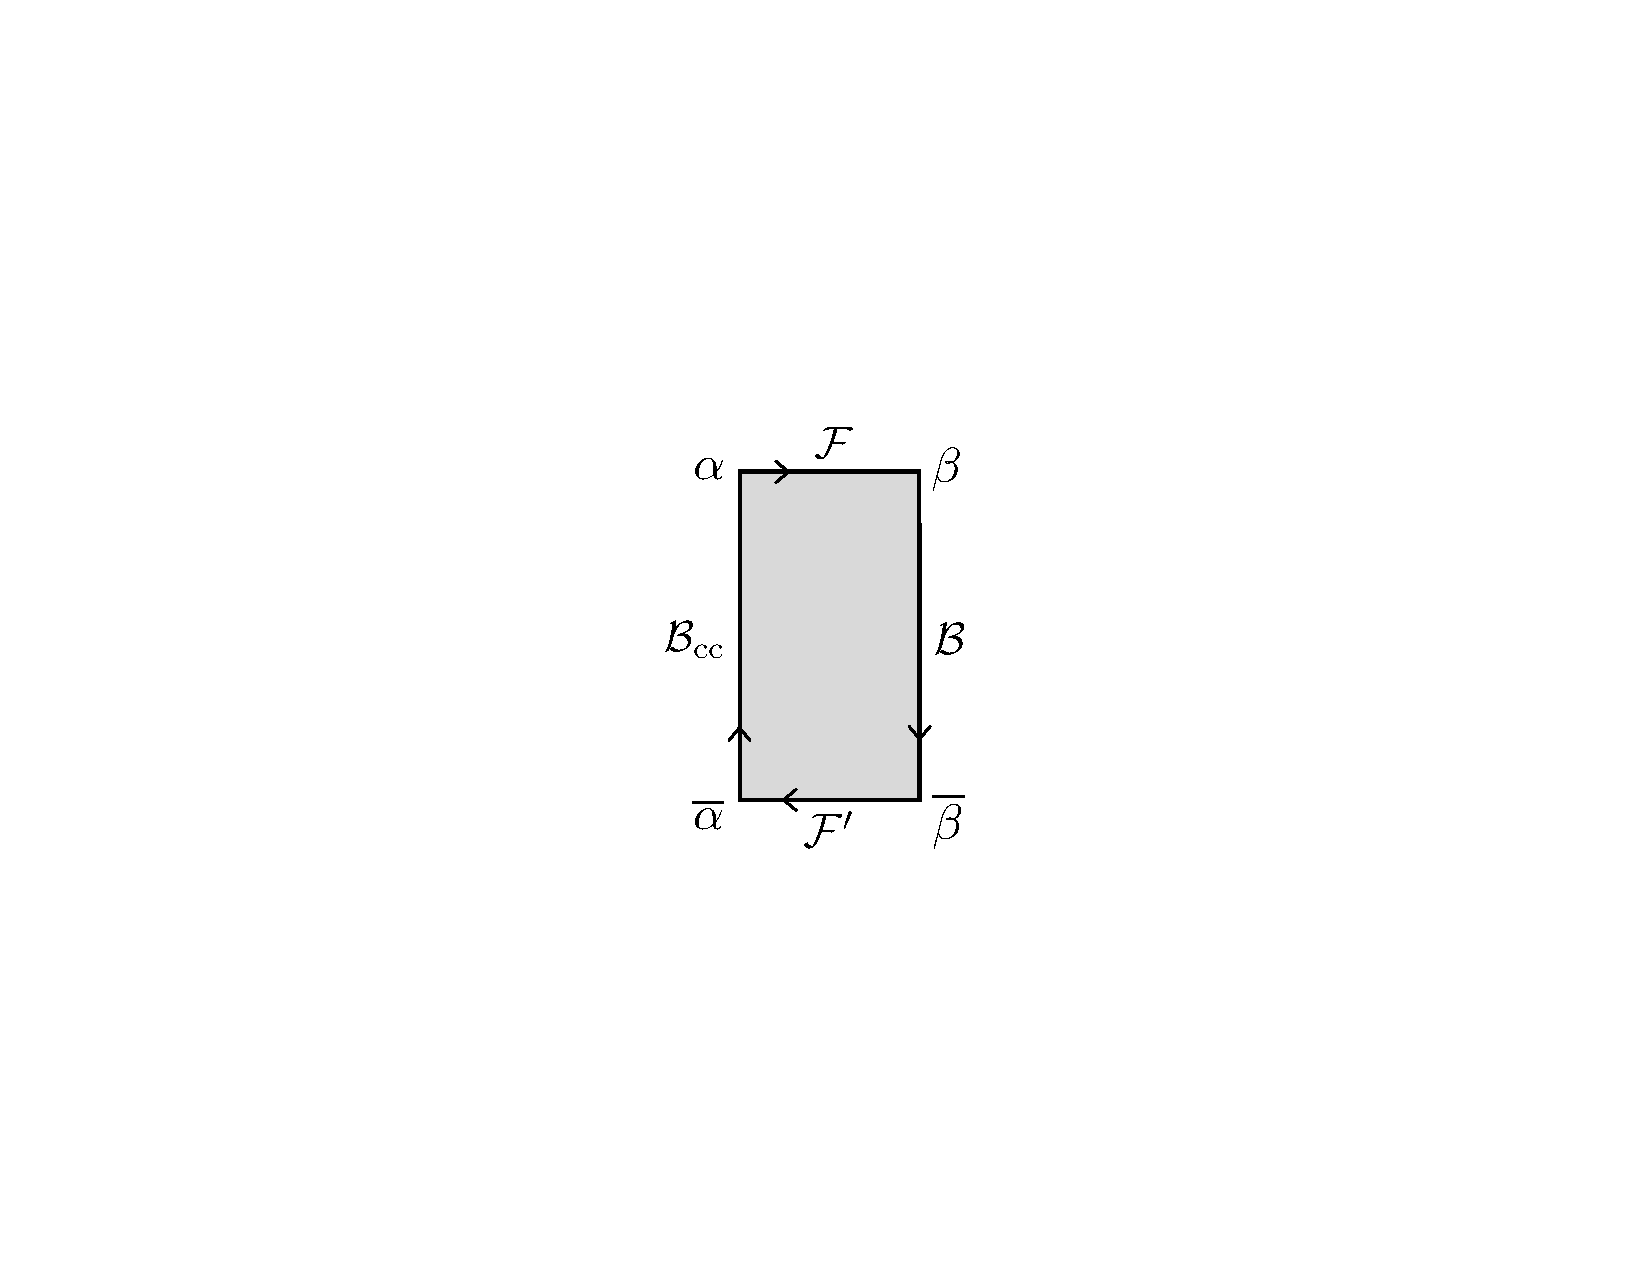
\includegraphics[width=0.36\textwidth]{figures/3.pdf}
 \caption{\small 由 $\F$ 与 $\F'$ 产生的态之间的内积，可通过此矩形上的路径积分计算。}
 \label{rectangle}
\end{figure}

我们断言：若 $w\ne w'$，则 $\langle\psi'(w';\alpha',\beta'),\psi'(w;\alpha,\beta)\rangle=0$。为证明这一点，利用 $A$-模型的二维拓扑不变性。我们通过讨论 Hilbert 空间 $\H=\Hom(\B_\cc,\B)$ 中从矩形底部传播到顶部的态来引入矩形；但也可等价地把矩形看作描述从左到右的传播。如图 \ref{secondone}(a) 所示，若利用拓扑不变性把矩形从左向右拉长，这第二种看法就很自然。图中从左向右传播的态是 $\Hom(\cF',\cF)$ 的元素。由于 $\cF$ 与 $\cF'$ 分别是支撑在 $F$ 与 $F'$ 上的拉格朗日 $A$-膜，计算 $\Hom(\cF,\cF')$ 的起点是交集 $F\cap F'$ 的上同调。但若 $w\ne w'$，则 $F\cap F'=\varnothing$，故 $\Hom(\cF,\cF')=0$，从而 $\langle\psi'(w';\alpha',\beta'),\psi'(w;\alpha,\beta)\rangle=0$。

\begin{figure}[htbp]
 \centering
 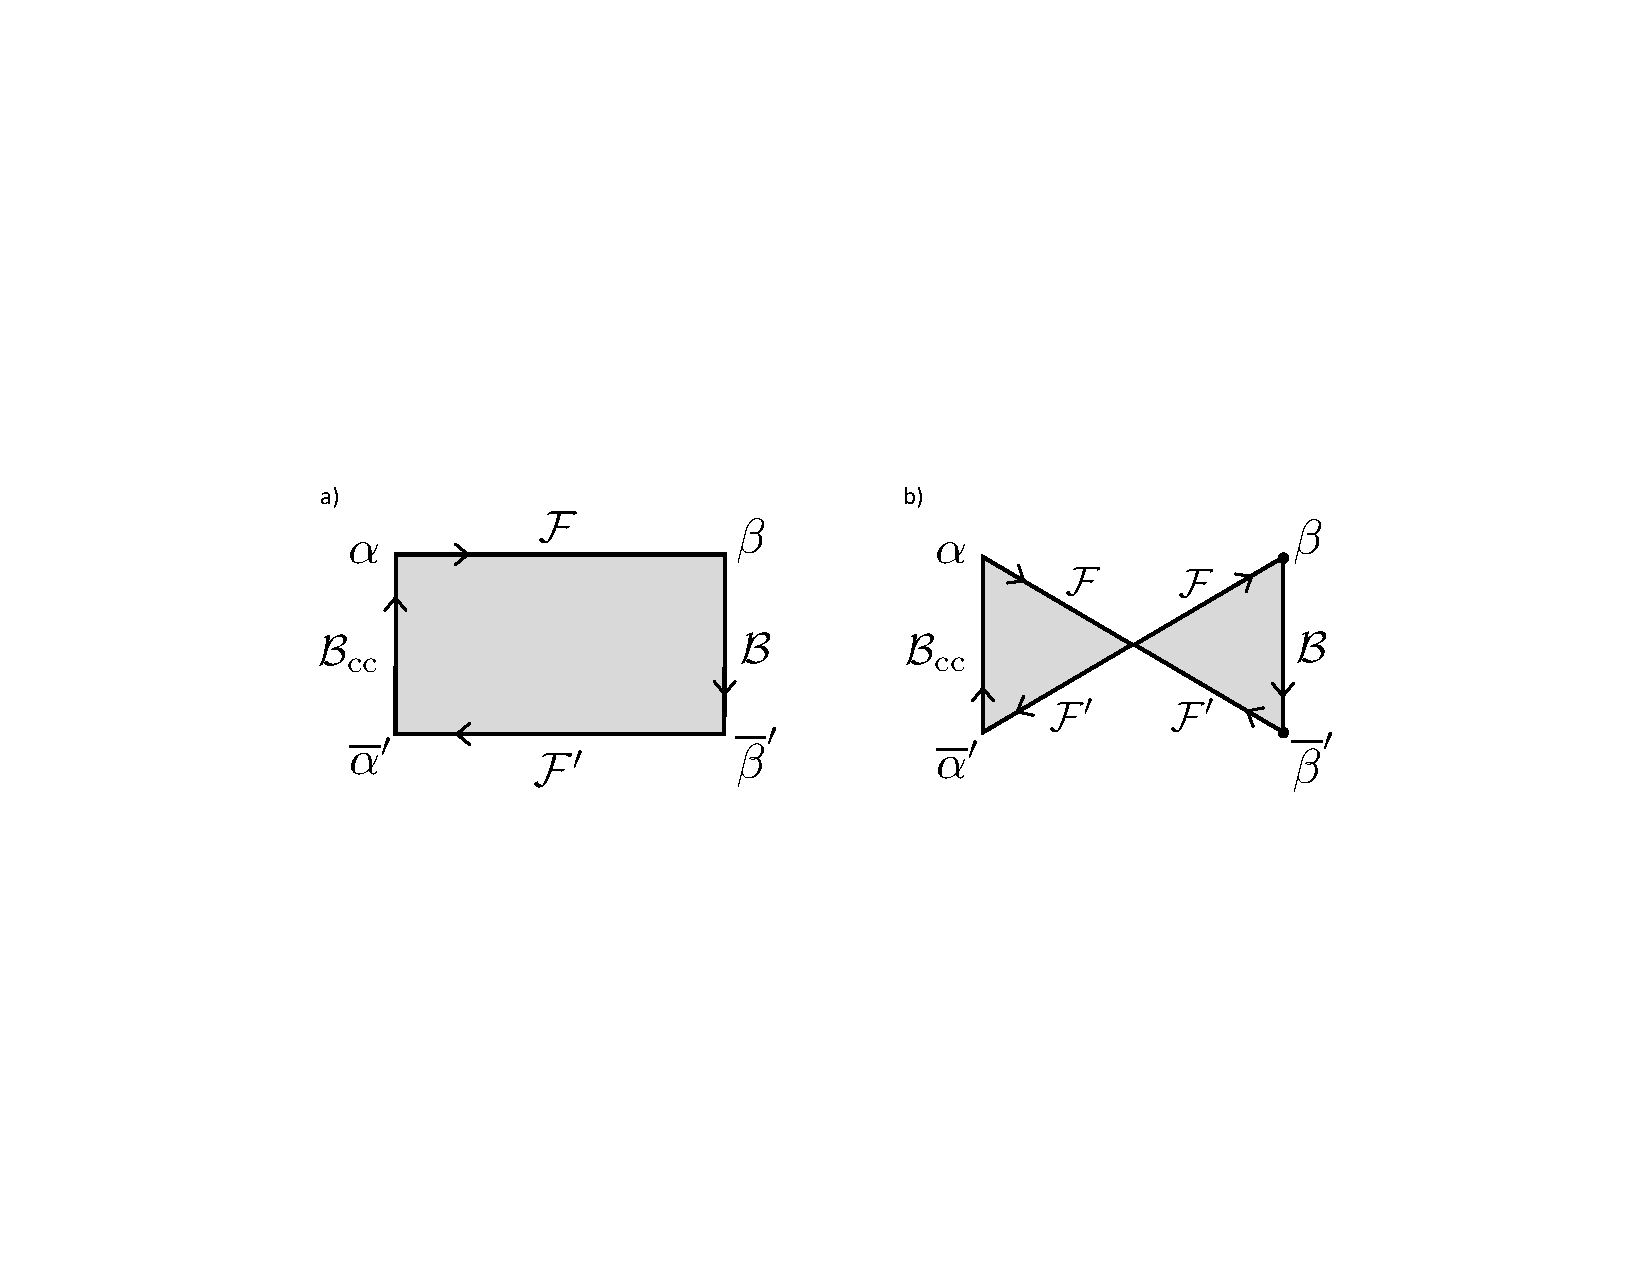
\includegraphics[width=0.72\textwidth]{figures/4.pdf}
 \caption{\small (a) 可把图 \ref{rectangle} 的矩形看作描述 $\Hom(\B,\B_\cc)$ 的元素从图底部到顶部的传播，或描述 $\Hom(\F',\F)$ 的元素从左到右的传播。把图形从左向右拉长会提示第二种解释。由于二维拓扑不变性，矩形的度量结构无关紧要。(b) 在某个极限下，矩形退化为两个在顶点粘合的三角形。穿过顶点的是 $\Hom(\F',\F)$ 中的一个态。可通过按 $\Hom(\F',\F)$ 的一组基态求和、并对每个基态计算两个三角形之积来求矩形的值。}
 \label{secondone}
\end{figure}

有时我们会在 $\Hom(\cF,\cF')$ 不为零的情形遇到类似矩形。为将来参考，注意这种矩形上的拓扑场论路径积分可这样计算：让矩形退化为在顶点粘合的一对三角形，如图 \ref{secondone}(b) 所示。左三角形涉及 $\B_\cc$ 与两个 $(B,A,A)$ 型膜；我们称这样的三角形为\textbf{全纯三角形}。右三角形涉及三个拉格朗日膜 $\cF,\cF',\B$；我们称之为\textbf{拉格朗日三角形}。

由于 $w\ne w'$ 时 $\langle\psi'(w';\alpha',\beta'),\psi'(w;\alpha,\beta)\rangle=0$，自然应把 $\psi'(w;\alpha,\beta)$ 视为支撑在点 $w\in N$ 处的 delta 函数态。若是如此，则预期 $\langle\psi'(w';\alpha',\beta'),\psi'(w;\alpha,\beta)\rangle$ 正比于 $\delta(w,w')$。遗憾的是，我们尚未找到通过研究矩形上路径积分来显式展示这个 delta 函数的方便办法。作为替代，我们将用其它方式探究 $\psi'(w;\alpha,\beta)$ 作为 delta 函数的解释。

回忆几何量子化的通常配方：把 $M=T^*N$ 作为余切丛量子化所得的 Hilbert 空间 $\H$，是 $N$ 上取值于预量子线丛 $\frL$ 的半密度空间。这意味着 $\H$ 的对偶空间是 $N$ 上取值于 $\frL$ 的对偶的半密度空间。在膜构造中，$\frL=\L^{-1}$，即 $\B$ 的 $\CP$ 丛之逆。

若 $f,g$ 分别是 $N$ 上取值于 $\L$ 与 $\L^{-1}$ 的半密度，则有自然双线性（非 Hermite）配对 $(f,g)=\int_Nfg$。故按几何量子化，$\H$ 的对偶应由 $N$ 上取值于 $\L$ 的半密度组成。来看能否把 $\psi'(w;\alpha,\beta)$ 解释为 $N$ 上支撑在 $w$ 处、取值于 $\L_w$ 的半密度。首先注意 $\psi'(w;\alpha,\beta)$ 正比于 $\beta$，而 $\beta$ 取值于 $\L_w$。还需理解如何把 $\psi'(w;\alpha,\beta)$ 解释为 $N$ 上支撑在 $w$ 处的半密度。

$N$ 上的密度丛是平凡实线丛，记作 $\K_N$。为简单起见假定 $N$ 可定向并取定定向。于是 $\K_N$ 同构于 $N$ 上最高次微分形式丛。若 $q^1,\cdots,q^n$ 是 $N$ 的局部坐标，其排序与 $N$ 的定向相容，则 $\K_N$ 可局部由 $\d q^1\d q^2\cdots\d q^n$ 平凡化，简记作 $\d\vec q$。由于 $\K_N$ 平凡，它有平凡平方根，记作 $\K_N^{1/2}$，可局部由截面 $(\d\vec q)^{1/2}$ 平凡化。

现在描述支撑在 $w$ 处的 delta 函数半密度。可选 $q^i$ 在点 $w$ 处为零。于是 $\delta^n(q^1,q^2,\cdots,q^n)$（简记 $\delta(\vec q)$）是支撑在 $w$ 处的 delta 函数。它自然理解为 $\K_N^{-1}$ 的截面，因为可与 $\K_N$ 的截面配对得数：$1=\int\d\vec q\,\delta(\vec q)$。支撑在 $w$ 处的 delta 函数半密度是 $(\d\vec q)^{1/2}\delta(\vec q)$ 的倍数，这是 $\K_N^{1/2}\K_N^{-1}=\K_N^{-1/2}$ 的截面。

另一方面，$\psi'(w;\alpha,\beta)$ 正比于 $\alpha=(\d\vec p)^{1/2}$。$T^*N$ 的辛结构在 $w$ 处切空间上确定自然测度 $\d\vec p\,\d\vec q$，其平方根是 $T^*N$ 上的自然半密度 $(\d\vec p)^{1/2}(\d\vec q)^{1/2}$。由于 $(\d\vec q)^{1/2}$ 取值于 $\K_N^{1/2}$，$(\d\vec p)^{1/2}$ 可解释为 $\K_N^{-1/2}$ 的截面，正如 $(\d\vec q)^{1/2}\delta(\vec q)$。

于是 $\psi'(w;\alpha,\beta)$ 自然地对应 $\H'$ 中如下 delta 函数元素：
\be\label{wacko}\psi'(w;\alpha,\beta)\sim(\d\vec q)^{1/2}\delta(\vec q)\cdot\beta.\ee
这个断言只是说：给定定义 $\psi'$ 所需的数据，即点 $w\in N$ 与波函数 $(\d\vec p)^{1/2}$、$\beta$，右端对象被典则地确定。而且这个等同与两边的 Hilbert 空间内积相容，至少若只考虑支撑在不同点的态之间的内积。

为进一步论证这个提议，可如下进行。设 $\Psi$ 是 $\H=\Hom(\B,\B_\cc)$ 中任一元，定义 $f(w,\alpha,\beta)=(\psi'(w;\alpha,\beta),\Psi)$，其中 $(\,,\,)$ 是 $\H$ 与 $\H'$ 之间的双线性 $A$-模型配对。令
\be\label{oko}\h\Psi(w)=f(w;\alpha,\beta)\sqrt{\d\vec q}\,\beta^{-1}.\ee
$\h\Psi(w)$ 是 $N$ 上取值于 $\L^{-1}$ 的半密度。$\h\Psi(w)$ 不依赖所作的任何选择，因为定义中显式的因子 $\sqrt{\d\vec q}$ 与 $\beta^{-1}$ 抵消了定义 $\psi'(w;\alpha,\beta)$ 时选取 $\sqrt{\d\vec p}$ 与 $\beta$ 的影响。故 $\h\Psi(w)$ 是几何量子化中（用 $M$ 作为余切丛所给的实极化）会定义的 Hilbert 空间 $\H_\gq$ 的元素。

于是我们找到了自然映射 $\H\to\H_\gq$，其中 $\H$ 是用复流形 $Y$ 对 $M$ 作膜量子化所定义的 Hilbert 空间，$\H_\gq$ 是把 $M$ 作为余切丛 $T^*N$ 作几何量子化所定义的 Hilbert 空间。我们预期这个映射是同构。为证明它，须证明任何与所有 $\psi'(w;\alpha,\beta)$ 正交的态 $\Psi$ 实际上为零。我们预期如此，但没有直接论证。如前所述，人们还希望有直接展示 $\langle\psi'(w;\alpha,\beta),\psi'(w';\alpha',\beta')\rangle$ 中 delta 函数的自然办法。

此分析中假定了 $N$ 可定向。若 $N$ 不可定向，推导要修改，因为 $\d\vec p$ 不是 $\K_N^{-1}$ 的截面，而是 $\K_N^{-1}\otimes\varepsilon$ 的截面，其中 $\varepsilon=\det T^*N$。与此相关，若 $N$ 不可定向，则膜 $\B$ 的 $\CP$ 丛不是曲率为 $-\omega$ 的酉线丛 $\L^{-1}$，而是 $\frL=\SS_0\otimes\L^{-1}$，其中 $\SS_0$ 是第 \ref{gq} 节描述的典则平坦 $\spinc$ 结构。我们预期这些微妙之处互相补偿，且即使 $N$ 不可定向，$\H$ 也是 $N$ 上取值于 $\L^{-1}$ 的 $L^2$ 半密度空间。但我们不试图给出细致论证。

作为所述构造的一个初等例子，考虑 $M=\R^2$。$M$ 上的仿射线性结构（即 $M$ 上什么是线性函数的概念，如第 \ref{problem} 节所解释）给出把 $M$ 复化为 $Y=\C^2$ 所需的信息：$M$ 上的实线性函数解析延拓为 $Y$ 上的全纯线性函数。为对 $M$ 作几何量子化，选取共轭线性函数 $p,q$ 使 $M$ 的辛形式为 $\d p\,\d q$。可把 $M$ 看作 $T^*\R$，$\R$ 以 $q$ 参数化；类似地可把 $Y$ 看作 $T^*\C$，$\C$ 以 $q$ 参数化（现在 $q$ 视为复变量）。于是所述构造表明：用这个实线性极化对 $M$ 作几何量子化，等价于用 $\H=\Hom(\B,\B_\cc)$ 作膜量子化，其中 $\B$ 是支撑在 $M$ 上的拉格朗日膜。由于膜量子化不依赖极化的选取，这表明用任何（与给定仿射线性结构相容的）实线性极化对 $M=\R^2$ 作几何量子化所得的 Hilbert 空间都自然同构。同样的逻辑适用于 $\R^{2n}$ 的量子化（一旦给定仿射线性结构）。我们重新得到了量子力学中一个著名事实：与仿射线性结构相容的不同实线性极化给出等价的量子化。\footnote{\label{maybe}更精确地说，这些不同线性极化给出的量子 Hilbert 空间自然等价，至多差一个整体符号。看到此符号出现的一个方式见脚注 \ref{cext}。在目前构造中，符号的来源可能在于波函数 $(\d\vec p)^{1/2}$ 的符号，我们没有以任何自然方式固定它。上述讨论中用 $N$ 的定向把 $K_W^{1/2}|_N$ 与 $N$ 上半密度空间等同，又引入了另一个符号。}

\subsection{扭余切丛}\label{shifted}

迄今为止，通过考虑 $Y=T^*W$ 及其标准全纯辛结构的情形，我们已能把膜量子化与几何量子化作比较，但只在相当特殊的情形。本节把构造推广到有时称为\textbf{扭余切丛}的对象。\footnote{关于此主题在更一般背景下的更多细节，见 \cite{Ginzburg}。}我们将看到，推广到扭余切丛使膜量子化与几何量子化之间更有趣的比较成为可能。

余切丛 $Y=T^*W$ 有全纯投影 $\pi:T^*W\to W$。纤维是拉格朗日子流形，都是 $\C^n$ 的拷贝，$n=\frac12\dim_\C Y$。此外，$W$ 可作为零截面全纯嵌入 $T^*W$。这个嵌入 $\iota:W\to T^*W$ 是 $\pi:T^*W\to W$ 的“截面”，即 $\pi\circ\iota=1$（等价地，对任意 $w\in W$，$\iota(w)\in\pi^{-1}(w)$）。

下面作推广：考虑具有上述所有性质、只差最后一条的复辛流形 $Y$。换言之，假定有全纯投影 $\pi:Y\to W$，$W$ 为某复流形。纤维是拉格朗日子流形，且同构于 $\C^n$。但投影 $\pi:Y\to W$ 可能没有全纯截面。

我们把这样的结构称为 $Y$ 的\textbf{全纯极化}，一般记作 $\varPi$。$\pi:Y\to W$ 的纤维就是 $\varPi$ 的叶。

对任意全纯线丛 $\L\to W$，我们将构造这样的结构。在 $\L$ 上取酉联络，其曲率 $\sff$ 为 $(1,1)$ 型；局部坐标下 $\sff=-\i\sum_{ij}f_{i\bar j}\d q^i\d\bar q^{\bar j}$。于是 $\Omega_0=\sum_i\d p_i\wedge\d q^i+\sff$ 是 $Y_0=T^*W$ 上的闭 2-形式，当然不是 $(2,0)$ 型。我们将说明如何修改 $Y_0$ 上的复结构，使 $\Omega$ 成为 $(2,0)$ 型且全纯。

描述 $\L$ 的一个显式办法是用开集 $\U_\alpha$ 覆盖 $W$，并在每个开集上选取 $\L$ 的平凡化。在此平凡化下，$\L$ 在 $\U_\alpha$ 上的截面就是全纯函数 $s_\alpha$。在交叠 $\U_\alpha\cap\U_\beta$ 上，局部平凡化由全纯转移函数 $e^{\v_{\alpha\beta}}$ 粘合；$\L$ 的整体截面 $s$ 是一族局部截面 $s_\alpha$，满足
\be\label{comsect} s_\alpha=e^{\v_{\alpha\beta}}s_\beta\ee
于 $\U_\alpha\cap\U_\beta$。$\L$ 上的 Hermite 内积于是在 $\U_\alpha$ 中由 $||s_\alpha||^2=e^{h_\alpha}\bar s_\alpha s_\alpha$ 定义，$h_\alpha$ 为实值函数。要求当 (\ref{comsect}) 成立时 $||s_\alpha||^2=||s_\beta||^2$ 于 $\U_\alpha\cap\U_\beta$，就给出 $h_\alpha$ 与 $h_\beta$ 的关系：
\be\label{hermrel} h_\alpha=h_\beta+2\Re\,\v_{\alpha\beta}. \ee
$\L$ 的曲率在区域 $\U_\alpha$ 中定义为
\be\label{curvdef} \sff=-\i\partial\bar\partial h_\alpha.\ee
式 (\ref{hermrel}) 说明它在交叠区域与 $\alpha$ 无关，故 $\sff$ 整体定义。此外，对 (\ref{hermrel}) 求导得
\be\label{ermrel}\partial_i h_\alpha=\partial_i h_\beta+\partial_i\v_{\alpha\beta}. \ee

我们要作的构造不仅对线丛有效，对线丛的复幂也有效，故先作推广。设 $\L_s$，$s=1,\cdots,k$，是 $W$ 上的全纯线丛，全纯转移函数为 $e^{\v_{s\,\alpha\beta}}$，Hermite 度量由局部函数 $h_{s\,\alpha}$ 定义。为把上一段的陈述推广到 $\L=\otimes_{s=1}^k\L_s^{\c_s}$（$\c_s$ 为复系数），定义曲率形式 $\sff=\sum_{s=1}^k\c_s\sff_s$，并令 $h_\alpha=\sum_{s=1}^k\c_s h_{s\,\alpha}$、$\v_{\alpha\beta}=\sum_s\c_s\v_{s\,\alpha\beta}$。上一段的公式无论 $\c_s$ 是否为整数都成立。特别地，在每个 $\U_\alpha$ 中，(\ref{curvdef}) 与 (\ref{ermrel}) 成立。若 $\c_s$ 不是整数，唯一出问题的地方是：在三重交叠中，$e^{\v_{\alpha\beta}+\v_{\beta\gamma}+\v_{\gamma\alpha}}$ 是常数但未必为 1。这不影响下文。

闭 2-形式 $\Omega=\sum_i\d p_i\d q^i+\sff$ 在 $Y_0=T^*W$ 的自然复结构下当然不是全纯的，甚至不是 $(2,0)$ 型。稍后我们将修改 $Y_0$ 的复结构使 $\Omega$ 全纯。把这个带修改后复结构的流形称为\textbf{扭余切丛}，记作 $Y$。$Y$ 仍带有全纯投影 $\pi:Y\to W$，纤维为 $\C^n$。

在解释此构造前，注意 $\sum_i\d p_i\d q^i=\d(\sum_i p_i\d q^i)$ 是恰当的，故 $\Omega=\sum_i\d p_i\d q^i+\sff$ 的上同调类就是 $\sff$ 的上同调类。这可表述为第一 Chern 类的陈述：若 $[\sff]$ 是形式 $\sff$ 的上同调类，则 $[\sff]/2\pi$ 表示第一 Chern 类 $c_1(\L)$。故
\be\label{jnko} [\Omega]=2\pi c_1(\L)=2\pi\sum_s \c_s c_1(\L_s). \ee
即使全纯投影 $\pi:Y\to W$ 没有全纯截面，它也总有光滑截面。而且 $Y$ 可缩到此截面上，而该截面是 $W$ 的拷贝。故可把式 (\ref{jnko}) 看作 $W$ 的上同调中的陈述。

例如，若 $W$ 紧，则由 Hodge 理论 $c_1(\L)$ 为 $(1,1)$ 型，故式 (\ref{jnko}) 表明 $[\Omega]$ 为 $(1,1)$ 型。又 $c_1(\L_s)$ 对一切 $s$ 为实，故若系数 $\c_s$ 为实，则 $[\Omega]$ 为实。这些是构造有趣量子化例子的便利条件。对量子化，我们要考虑支撑在纤维化 $\pi:Y\to W$ 的非全纯截面 $M$ 上的膜，并要求 $M$ 对 $\Im\Omega$ 为拉格朗日、对 $\Re\Omega$ 为辛。为使这样的 $M$ 存在，条件 $[\Im\Omega]=0$ 是必要的。$[\Re\Omega]$ 非零并非构造例子所必需，但许多最有意思的例子都有 $[\Re\Omega]\ne0$。

为定义新复结构，只须说：在 $T^*\U_\alpha$ 中，函数
\be\label{newc} p_{\alpha\,i}=p_i+\i\partial_i h_\alpha(q,\bar q) \ee
是纤维上的全纯坐标；我们定义新的全纯结构，使 $p_{\alpha\,i}$ 与 $q^j$ 全纯，而非 $p_i$ 与 $q^j$。这个定义已安排好，使得在 $T^*\U_\alpha$ 中
\be\label{ewc} \Omega=\sum_i\d p_{\alpha\,i}\d q^i, \ee
故 $\Omega$ 在 $T^*\U_\alpha$ 中为 $(2,0)$ 型且全纯。当然，$\Omega$ 整体定义，此式对一切 $\alpha$ 成立。此外，由式 (\ref{ermrel})，在交叠区域 $\U_\alpha\cap\U_\beta$ 中
\be\label{newco} p_{\alpha\,i}=p_{\beta\,i}+\i\partial_i\v_{\alpha\beta},\ee
其中 $\v_{\alpha\beta}$ 全纯。于是，虽然 $p_{\alpha\,i}\ne p_{\beta\,i}$，但在 $T^*(\U_\alpha\cap\U_\beta)$ 上使 $p_{\alpha\,i}$ 与 $q^j$ 全纯的复结构，与在该开集上使 $p_{\beta\,i}$ 与 $q^j$ 全纯的复结构相同。因此，我们在各开集 $T^*\U_\alpha$ 上定义的复结构在所有交叠上一致，拼成 $T^*W$ 上的新复结构。这样就定义了新复流形 $Y$，它作为光滑流形与原余切丛相同。在 $Y$ 上，$\Omega$ 全纯且为 $(2,0)$ 型，故 $Y$ 是复辛流形。

式 (\ref{newco}) 与式 (\ref{transpo}) 形式相同，只需取 $w=v/\hbar$，故先前的讨论适用。于是，若能假定量子算符 $\h p,\h q$ 的变换律与经典函数 $p,q$ 的变换律相同，则由第 \ref{cotangent} 节的讨论可推出：$\Hom(\B_\cc,\B_\cc)$ 由作用在 $\L=\otimes_{s=1}^k\L_s^{\lambda_s}$（$\lambda_s=\c_s/\hbar$）上的全纯微分算符组成。$Y$ 的几何由参数 $\c_s$ 控制；若固定 $Y$ 的几何而改变 $\hbar$，则指数 $\lambda_s$ 为 $1/\hbar$ 阶。

这不是正确答案，因为它忽略了第 \ref{cotangent} 节与第 \ref{lagbr} 节分析过的量子效应。即使经典公式 (\ref{newco}) 中 $\v_{\alpha\beta}=0$（例如 $Y=T^*W$ 带其通常辛结构时），也有量子贡献，使得 $\Hom(\B_\cc,\B_\cc)$ 由作用在 $K_W^{1/2}$ 的截面（而非函数）上的全纯微分算符组成。

自然猜测：$\h p$ 变换律中的经典效应与量子效应应当相加。此时 $\Hom(\B_\cc,\B_\cc)$ 将由作用在张量积 $K_W^{1/2}\otimes\L$ 上的全纯微分算符组成。

为论证此答案，只须注意问题有伸缩律：$q$ 不变，而 $p$、$\hbar$、$v$ 均以次数 1 伸缩。故在保持伸缩对称的量子化中，$\h p$ 的变换只能是 $\hbar$ 与 $\phi$ 的线性函数，从而把经典效应与量子效应相加、取 $K_W^{1/2}$ 与 $\L$ 的张量积是正确的。

最后讨论对给定 $W$，如何分类这样构造的 $Y$。设 $W$ 紧。则由 Hodge 理论，任何满足 $c_1(\RR)$ 以复系数为零的全纯线丛 $\RR\to W$ 都容许平坦联络。对此类 $\RR$，作用在 $\L$ 上的全纯微分算符与作用在 $\RR\otimes\L$ 上的相同。因此，若 $W$ 紧，用此构造能作出的复辛流形 $Y$ 完全由复系数的 $c_1(\L)$ 分类，换言之（由式 (\ref{jnko})）由上同调类 $[\Omega]$ 分类。对非紧 $W$，一般不是这样；可以有拓扑平凡但不容许平坦联络的全纯线丛 $\RR\to W$。故非紧情形一般更复杂。

\subsection{一个例子}\label{example}

本节详细算一个扭余切丛的简单例子。我们只讨论形变量子化，把量子化推迟到第 \ref{scbq} 节。

所考虑的例子是式 (\ref{cosu}) 中已引入的复辛流形 $Y$。它由方程\footnote{稍后我们将令 $\j=\hbar j$，最终令 $\hbar=1$，把 $\j$ 换成 $j$。}
\be\label{inco} x^2+y^2+z^2=\j^2 \ee
描述，全纯辛形式为
\be\label{nco}\Omega=\frac{\d x\,\d y}{z}. \ee

该方程与辛形式在 $G=\SO(3,\C)=\PGL(2,\C)$ 对三元组 $x,y,z$ 的显然作用下不变。确实，$Y$ 是 $G$ 的余伴随轨道。它可看作 $G$ 的 Lie 代数 $\g$ 中行列式为 $-\j^2$ 的元素 $T$ 构成的子空间。任何这样的元素可写成
\be\label{pok} T=\begin{pmatrix} z & x+\i y \cr x-\i y & -z\end{pmatrix} \ee
其中 $x,y,z$ 满足式 (\ref{inco})。这样的 $T$ 的特征值为 $\j$ 与 $-\j$，故特征值问题
\be\label{ok}T\begin{pmatrix} q \cr 1\end{pmatrix}=-\j\begin{pmatrix} q \cr 1\end{pmatrix},\qquad T\begin{pmatrix} q' \cr 1\end{pmatrix}=\j\begin{pmatrix} q' \cr 1\end{pmatrix}
\ee
有唯一解，$q,q'\in\C\cup\infty$：
\begin{align}\label{pola} q& = -\frac{x+\i y}{\j+z}=-\frac{\j-z}{x-\i y}\cr
                     q'& = \frac{x+\i y}{\j-z}=\frac{\j+z}{x-\i y}. \end{align}
显然 $q$ 与 $q'$ 在 $\j\leftrightarrow-\j$ 下互换。$q$ 或 $q'$（加上一个无穷远点）参数化 $W=\bCP^1$ 的拷贝，它就是 $T$ 所作用的二维向量空间的射影化。显然 $G$ 将以熟悉的分数线性变换 $q\to(aq+b)/(cq+d)$、$q'\to(aq'+b)/(cq'+d)$（$ad-bc=1$）作用在 $W$ 上。

$Y$ 中没有 $q=q'$ 的点，因为 $T$ 的两个特征向量总不相同。这是唯一的约束；任何一对不同的 $q,q'\in\bCP^1$ 都确定唯一的 $T$，可由式 (\ref{pola}) 解出 $x,y,z$ 得到。$\bCP^1$ 中一点的补集是 $\C$ 的拷贝。故给定 $q$ 时 $q'$ 的可能值参数化一个 $\C$；类似地，给定 $q'$ 时 $q$ 的可能值参数化一个 $\C$。于是 $Y$ 有两个全纯极化：一个的叶由 $q$ 的选择标号（并由满足 $q'\ne q$ 的 $q'$ 参数化），另一个的叶由 $q'$ 标号（并由满足 $q\ne q'$ 的 $q$ 参数化）。把由 $q$ 与 $q'$ 参数化的全纯极化分别记作 $\varPi$ 与 $\varPi'$。

简单计算给出用\footnote{下式中的因子 $1/(q-q')^2$ 并不真正表示 $\Omega$ 的极点，因为如前所述 $q$ 与 $q'$ 总不相同。}$q$ 与 $q'$ 表示辛形式的公式：
\be\label{shortform}\Omega=2\i\j\frac{\d q\d q'}{(q-q')^2}.\ee
也许出乎意料，$q$ 与 $q'$ 的共轭变量可取为相等，因为若
\be\label{momform} p=p'=-\frac{2\i\j}{q-q'}, \ee
则
\be\label{canform}\Omega=\d p\,\d q=\d p'\d q'. \ee

为整体描述此情形，用两个开集 $\U$ 与 $\t\U$ 覆盖 $\bCP^1$，其中 $\U$ 是 $\bCP^1$ 中无穷远点的补集，$\t\U$ 是原点的补集。$\U$ 中的好变量是 $q,q'$；$\t\U$ 中的好变量可由分数线性变换得到：$\t q=-1/q$，$\t q'=-1/q'$。共轭变量为
\be\label{ranform} \t p=\t p'=-\frac{2\i\j}{\t q-\t q'}. \ee
由这些公式可得
\be\label{anform}p=\t q^2\t p+2\i\j\t q=\t q^2\t p-\frac{2\i\j}{q}. \ee
为与一般公式 (\ref{transp}) 比较，注意本例中 $W=\bCP^1$ 的复维为 1，故式 (\ref{transp}) 中的指标 $i,k$ 可省略。我们只用两个开集覆盖 $W$，故 $q,p$ 对应 (\ref{transp}) 中的 $q_\alpha,p_\alpha$，$\t q,\t p$ 对应 $q_\beta,p_\beta$。函数 $\t q^2$ 扮演矩阵 $M$ 的角色；最后，为把 (\ref{anform}) 写成 (\ref{transp}) 的形式，应把 $-2\i\j/q$ 写成 $\i\hbar\partial_q u$，$u$ 为某全纯函数。于是\footnote{函数 $u$ 不是单值的；这是我们用交叠非单连通的开集覆盖 $W$ 所付的代价。第 \ref{shifted} 节的程序会告诉我们用更多、交叠可缩的开集覆盖 $W=\bCP^1$。那时可定义总为单值、但在三重交叠中不满足 $S_{\alpha\beta}S_{\beta\gamma}S_{\gamma\alpha}=1$（除非 $2j\in\Z$）的转移函数。沿这些线索的推导会更长。}$u=-2j\log q$，其中已令 $\j=\hbar j$。然后试图把 $e^u$ 解释为线丛 $\L$ 的转移函数。此时 $e^u=q^{2j}$。它单值当且仅当 $2j\in\Z$，故只有这种情形 $\L$ 才是真正的线丛；对其他 $j$ 值，$\L$ 实际上是线丛的复幂。当 $2j\in\Z$ 时所得的线丛 $\L$ 是熟悉的：在区域 $\t\U$ 中为 1 的截面（在上述 $\t p$ 公式隐含的平凡化下），在区域 $\U$ 中为 $e^u=q^{2j}$（在 $p$ 公式隐含的平凡化下）。该截面在原点有 $2j$ 阶零点、无极点，故 $\L$ 就是通常所说的 $\O(2j)$。无论 $2j\in\Z$ 与否，我们都用记号 $\O(2j)$；要点始终是：作用在 $\O(2j)$ 上的微分算符有定义——我们将写出显式公式——无论 $\O(2j)$ 是否作为线丛存在。

现在讨论空间 $Y$ 上的典范余各向同性 $A$-膜 $\B_\cc$。按一般讨论，$\Hom(\B_\cc,\B_\cc)$ 是作用在 $K_W^{1/2}\otimes\L$ 上的全纯微分算符层。对 $W=\bCP^1$，$K_W\cong\O(-2)$，$K_W^{1/2}\cong\O(-1)$。故 $K_W^{1/2}\otimes\L=\O(2j-1)$。于是预期 $\Hom(\B_\cc,\B_\cc)$ 是 $\bCP^1$ 上作用在 $\O(2j-1)$ 上的全纯微分算符代数。在导出此陈述的某些阶段，我们对 $\Hom(\B_\cc,\B_\cc)$ 作了层化（尽管从物理观点看这一步未必完全自然），但在最终陈述中无需层化。$\Hom(\B_\cc,\B_\cc)$ 就是作用在 $\O(2j-1)$ 上的整体定义的全纯微分算符代数。

然而注意，我们一开始有两个同样好的 $Y$ 的全纯极化，相差 $j\to-j$。若在分析最后一步使用第二个，就会把 $\Hom(\B_\cc,\B_\cc)$ 等同于作用在 $\O(-2j-1)$ 上的整体全纯微分算符代数。因此预期这两个代数同构。确实如此，稍后便知。

$\bCP^1$ 上作用在 $\O(2j-1)$ 上的整体微分算符代数由\footnote{下文令 $\hbar=1$。式 (\ref{throps}) 中的公式在可取这些算符的线性组合并加常数的意义下唯一确定；我们作了方便的选择。}
\begin{align}\label{throps}    t_- & = -\frac{\d}{\d q} \cr
                     t_3 & = q\frac{\d}{\d q}-j+\frac{1}{2} \cr
                      t_+ & = q^2\frac{\d}{\d q}-(2j-1)q \end{align}
生成。这些算符满足 $\mathfrak{sl}(2)$ Lie 代数 $\g$ 的熟悉换位关系：
\be\label{usrel} [t_3,t_\pm]=\pm t_\pm,\qquad [t_+,t_-]=2t_3. \ee
为验证这些算符整体全纯，我们从 $q$ 变换到 $\t q=-1/q$ 并共轭以 $\O(2j-1)$ 的转移函数，检查 $q=\infty$ 处的行为。例如 $t_+=q^2\frac{\d}{\d q}-(2j-1)q$ 变为 $\t q^{2j-1}\left(\frac{\d}{\d\t q}+\frac{2j-1}{\t q}\right)\t q^{-(2j-1)}=\frac{\d}{\d\t q}$，在 $\t q=0$ 处全纯。由于项 $\frac{2j-1}{\t q}$ 的精确系数，极点项抵消了。总之
\begin{align}\label{agrops} t_-& = -\t q^2\frac{\d}{\d\t q}+(2j-1)\t q\cr
                                           t_3& = -\t q\frac{\d}{\d\t q}+j-\frac{1}{2} \cr
                                            t_+ & = \frac{\d}{\d\t q}. \end{align}
算符 $t_+,t_-,t_3$ 代数独立，只差一个关系：把 $\g$ 的二次 Casimir 算符等于一个 $c$-数：
\be\label{eqrel} \frac{1}{2}(t_+t_-+t_-t_+)+t_3^2=j^2-\frac{1}{4}. \ee
它在 $j\to-j$ 下具有预期的对称性。$K_W^{1/2}$ 的平移对得到此对称性至关重要。

算符 $t_+,t_-,t_3$ 是 $Y$ 上全纯函数代数生成元 $x,y,z$ 的量子版本。例如，公式 $p=-2\i j/(q-q')=\i(x-\i y)$ 连同 $p=-\i\d/\d q$ 表明 $t_-=-\d/\d q$ 对应 $x-\i y$。更一般地，梳理上述 $x,y,z$ 与 $p,q$ 的关系，得
\begin{align} \label{correspo} x-\i y &\to t_- \cr
                                             x+\i y &\to t_+ \cr
                                             z& \to t_3. \end{align}
于是 Casimir 关系 (\ref{eqrel}) 是原经典关系 $x^2+y^2+z^2=j^2$ 的量子形变版本。

以上只讨论了形变量子化。第 \ref{scbq} 节将加入拉格朗日 $A$-膜并分析量子化。届时 $Y$ 的一个反全纯对合很重要。若 $\j^2$ 为实，则 $Y$ 有显然的反全纯对合 $\tau:(x,y,z)\to(\bar x,\bar y,\bar z)$。回顾式 (\ref{pola}) 的出发点可知，$\tau$ 交换两个全纯极化 $\varPi$ 与 $\varPi'$（确切地说，$\tau$ 把 $\varPi$ 中给定 $q$ 值的叶映到 $\varPi'$ 中 $q'=-1/\bar q$ 的叶）。同一个复流形 $Y$（仍设 $\j^2$ 实）还有另一个反全纯对合 $\t\tau:(x,y,z)\to(\bar x,-\bar y,-\bar z)$，也把 $\Omega$ 映到 $\bar\Omega$。为写出更清楚的公式，方便的是通过重新定义 $(x,y,z)\to(x,\i y,\i z)$ 把 $\t\tau$ 拉回到 $\tau$。定义 $Y$ 的方程变为
\be\label{nuuxx} x^2-y^2-z^2=j^2, \ee
辛形式仍为 $\Omega=\d x\,\d y/z$。我们考虑这个流形 $Y'$，配以复共轭 $x,y,z$ 的原反全纯对合 $\tau$。当然，纯粹作为复流形，$Y'$ 与 $Y$ 等价，故仍有两个全纯极化。但有个有趣的差别。对 $j^2>0$，两个全纯极化仍被 $\tau$ 交换。但若 $j^2=-s^2$ 为负，则两个全纯极化各自 $\tau$-不变。方程 $x^2-y^2-z^2=-s^2$ 等价于说矩阵
\be\label{uvux}T'=\begin{pmatrix} z & x-y \cr -x-y & -z\end{pmatrix}\ee
的特征值为 $\pm s$。解特征值问题
\be\label{eipro}T'\begin{pmatrix} q \cr 1\end{pmatrix}=-s\begin{pmatrix} q \cr 1\end{pmatrix},\qquad T'\begin{pmatrix} q' \cr 1\end{pmatrix}=s\begin{pmatrix} q' \cr 1\end{pmatrix},\ee
得
\begin{align}\label{horiz} q & = -\frac{x-y}{z+s}=-\frac{z-s}{x+y} \cr
 q'& = -\frac{x-y}{z-s}=-\frac{z+s}{x+y}, \end{align}
它们定义两个全纯极化 $\varPi$ 与 $\varPi'$。由于这些公式完全实，$\varPi$ 与 $\varPi'$ 各自 $\tau$-不变。更确切地说，$\tau$ 通过 $q\to\bar q$ 作用在 $\varPi$ 上，固定实 $q$ 的叶并将其余叶成对交换；对 $\varPi'$ 类似。

\subsection{应用于量子化}\label{scbq}

现在讨论如何把全纯极化用于量子化。考虑第 \ref{amo} 节引入的情形：$Y$ 是复辛流形，复结构为 $I$，全纯辛形式为 $\Omega$，并带反全纯对合 $\tau$ 使 $\tau^*(\Omega)=\bar\Omega$；$M$ 是 $\tau$ 不动点集的一个分支，对 $\omega_J=\Re\Omega$ 为辛的（同时对 $\omega_K=\Im\Omega$ 必然为拉格朗日的）。假定 $Y$ 有全纯极化 $\varPi$，其叶是某全纯映射 $\pi:Y\to W$ 的纤维，$W$ 为某复流形。我们要理解 $\varPi$ 的存在对 $M$ 的膜量子化意味着什么。

由于 $Y$ 被 $\varPi$ 的叶分层，每点 $p\in M$ 含于唯一的叶 $F_p$。$F_p$ 对 $\Omega$ 为拉格朗日，故对 $\omega_J$ 也是。于是 $\omega_J$ 限制到 $F_p\cap M$ 为零。因此 $F_p\cap M$ 在 $M$ 中至多是中间维的。若它是中间维的，它就是 $M$ 的拉格朗日子流形。假定对每个与 $M$ 相交的 $\varPi$ 叶都如此，且所有这些拉格朗日子流形都是 $\R^n$ 的拷贝。那么形如 $F_p\cap M$ 的 $M$ 的拉格朗日子流形定义 $M$ 的一个实极化 $\P$。在此情形，我们将证明 $M$ 的膜量子化等价于用实极化 $\P$ 作几何量子化。

设 $N$ 是 $\P$ 的叶空间。它是 $W$ 中参数化与 $M$ 相交的 $\varPi$ 叶的子空间。$N$ 中的点对应 $\varPi$ 的叶 $F$，使 $F\cap M$ 的实维数为 $n$，故 $F\cap M$ 在 $F$ 中是中间维的。$F\cap M$ 是全实的（因 $M$ 是全实的），故 $F$ 是 $F\cap M$ 的复化。由于 $F\cap M$ 为 $\tau$-不变，而 $F$ 是 $F\cap M$ 的复化，$F$ 被 $\tau$ 映到自身（虽非逐点）。

再由维数计数可知 $N$ 在 $W$ 中是中间维的；$N$ 的实维数为 $n=\frac12\dim_\R M=\frac12\dim_\C Y$，与 $W$ 的复维数相同。$N$ 参数化 $W$ 的一个中间维全实子空间，故 $W$ 可看作 $N$ 的复化。$\tau$ 作为 $W$ 的反全纯对称作用，保持 $N$ 不动。$W$ 中不属于 $N$ 的点对应不与 $M$ 相交的 $\varPi$ 叶；至少在 $N$ 的邻域内，这样的叶被 $\tau$ 成对交换。特别地，全纯极化 $\varPi$ 是 $\tau$-不变的，尽管并非每片叶都被 $\tau$ 映到自身。

一个初等例子：取 $Y=\C^2$，用复变量 $p,q$ 参数化，$\Omega=\d p\,\d q$。令 $\tau$ 由 $(p,q)\to(\bar p,\bar q)$ 作用，不动点集为 $M$。把 $p,q$ 按实部与虚部展开：$p=p_1+\i p_2$，$q=q_1+\i q_2$。$M$ 是由 $p_1,q_1$ 参数化的 $\R^2$ 拷贝。$Y$ 有全纯极化 $\varPi$，其叶为 $q=b$，$b$ 为复参数，标志叶的选择。于是叶空间 $W$ 是 $\C$ 的拷贝。$\tau$ 把 $q=b$ 的叶映到由 $\bar q=b$ 即 $q=\bar b$ 定义的叶；$\tau$-不变的叶是 $b$ 为实的叶。故 $\tau$ 通过复共轭作用在 $W\cong\C$ 上，固定实轴 $N$。$N$ 中的点对应与 $M$ 交于 $\R$ 的拷贝的 $\varPi$ 叶；这些 $\R$ 的拷贝就是 $M$ 的实极化 $\P$ 的叶。

一个稍精致的例子：考虑式 (\ref{nuuxx}) 的复辛流形 $Y'$，取 $j^2<0$，使 $s$ 为实。$M$ 由同一方程且 $x,y,z$ 为实描述。式 (\ref{horiz}) 给出 $Y'$ 的两个不同全纯极化 $\varPi$ 与 $\varPi'$，一个由 $q$ 参数化，一个由 $q'$ 参数化。$\tau$ 把 $\varPi$ 映到自身，也把 $\varPi'$ 映到自身。与 $M$ 有非空交集的 $\varPi$ 或 $\varPi'$ 的叶，是 $q$ 或 $q'$ 为实的叶。这些叶给出 $M$ 的两个实极化 $\P$ 与 $\P'$。与 $\varPi$、$\varPi'$ 相应的两个投影 $\pi,\pi':Y\to W\cong\bCP^1$ 限制到 $M$ 上，给出投影 $\pi,\pi':M\to N=\RP^1$，$N$ 由 $q$ 或 $q'$ 加上一个无穷远点参数化。

现在考虑相当不同的可能性。若 $F$ 是全纯极化 $\varPi$ 的叶，则 $F$ 与 $M$ 在 $Y$ 中都是中间维的，故 $F\cap M$ 自然可能只由一点组成（由若干点组成也自然，但我们不考虑这种情形）。假定对每个 $\varPi$ 叶，$F\cap M$ 至多是一点。于是投影 $\pi:Y\to W$ 限制为 $M$ 到其像 $\pi(M)$ 的同构（$\pi(M)$ 可能只是 $W$ 的一部分，后面例子会看到）。由于 $W$ 是复流形，这给 $M$ 一个复结构，记作\footnote{此记号的理由是：若 $Y$ 的复结构（我们称为 $I$）可延拓为带附加复结构 $J,K$ 的超 Kähler 结构，则 $\J$ 有时就是 $J$ 在 $M$ 上的限制。}$\J$。在复结构 $\J$ 下，$M$ 上的全纯函数是 $W$ 上全纯函数经 $\pi^*$ 的拉回。注意：若 $V$ 是 $Y$ 上切于 $\varPi$ 叶的向量场（不必全纯），则 $V$ 在 $W$ 上投影为零，故从 $W$ 拉回的函数的 $V$ 方向导数为零：
\be\label{looj} \mathcal L_V\cdot\pi^*(f)=0. \ee
在此情形，$\J$ 是几何量子化意义下 $M$ 的复极化，因为 $\omega_J|_M=\Re\Omega|_M$ 对 $\J$ 为 $(1,1)$ 型。为看出这点，令 $T_pM$ 为 $M$ 在 $p\in M$ 处的切空间，$T_{p,\C}M=T_{p,M}\otimes_\R\C$ 为其复化。考虑分解 $T_{p,\C}M=T^{1,0}_{p,\C}M\oplus T^{0,1}_{p,\C}M$，两个子空间分别是 $M$ 的全纯与反全纯复化切方向（在复结构 $\J$ 下）。作为向量空间，$T^{0,1}_{p,\C}M$ 可自然等同于 $T_pF_p$，即 $M$ 在含 $p$ 的 $\varPi$ 叶 $F_p$ 中的切空间（这由式 (\ref{looj}) 推出：$M$ 上的全纯函数被 $T_pF_p$ 方向的导数零化）。由于 $F_p$ 对 $\Omega$ 为拉格朗日，这说明 $\Omega|_M$ 的 $(0,2)$ 部分在复结构 $\J$ 下为零。连同 $M$ 对 $\Im\Omega$ 为拉格朗日，可知 $\Re\Omega|_M$ 的 $(2,0)$ 与 $(0,2)$ 部分都为零，故 $\Re\Omega|_M$ 为 $(1,1)$ 型。

$Y$ 的反全纯对合 $\tau$ 把 $\varPi$ 映到全纯极化 $\varPi'=\tau(\varPi)$。$\tau$ 把全纯变化的 $\varPi$ 叶族映到反全纯变化的 $\varPi'$ 叶族，故它反转 $M$ 上诱导的复结构。特别地，$\varPi$ 与 $\varPi'$ 总是不同。若 $\omega$ 在 $\varPi$ 诱导的复结构 $\J$ 下正定（即 $\J$ 给出几何量子化意义下的复 Kähler 极化），则它在 $\varPi'$ 诱导的复结构 $-\J$ 下负定。

在此情形，我们将在第 \ref{branecp} 节论证：$M$ 的膜量子化（至少作为向量空间，暂且不管 Hilbert 空间结构）与用 $\varPi$ 诱导的 $M$ 的复极化作几何量子化一致。Hilbert 空间结构一般不同，第 \ref{flatg} 节的例子会说明这一点。

但先看几个由 $Y$ 的全纯极化诱导 $M$ 的复极化的例子。初等例子仍取 $Y=\C^2$，$p,q,\Omega,\tau,M$ 同前。但现在用方程 $q+\i p=b$ 定义 $\varPi$ 的叶，$b$ 仍为标志叶选择的常数。这样的叶与 $M$ 交于唯一点 $q_1+\i p_1=b$。故此时 $M$ 获得一个复结构，其中 $z=q_1+\i p_1$ 全纯。切于叶 $q+\i p=b$ 的向量场是 $\frac{\partial}{\partial q}+\i\frac{\partial}{\partial p}$，沿 $M$ 解释为 $2\frac{\partial}{\partial\bar z}$。$\varPi$ 的 $\tau$-共轭是极化 $\varPi'$，其叶由 $q-\i p=b$ 定义，$b$ 仍为参数。诱导的复结构是使 $\bar z=q_1-\i p_1$ 全纯的那个。

稍微妙的例子：考虑第 \ref{example} 节研究过的复流形 $x^2+y^2+z^2=\j^2$，取 $\j^2>0$。$M$ 是 $x,y,z$ 为实的子流形。对实 $x,y,z$，式 (\ref{pok}) 的矩阵 $T$ 是 Hermite 的。特征值为 $\j,-\j$ 的 $2\times2$ Hermite 矩阵在给定一个特征向量时唯一确定，而可通过给定 $q$ 或 $q'$ 来指定。于是 $\varPi$ 或 $\varPi'$ 的任何叶都与 $M$ 交于唯一点。构造的 $\SO(3)$ 对称性保证 $M$ 上诱导的复结构（差一符号）就是 $M\cong S^2\cong\bCP^1$ 的自然复结构。但事实上符号相反。看出这点的一个办法是注意簇 $Y$ 有全纯对合 $\zeta:(x,y,z)\to(-x,-y,-z)$。这个对合（它改变全纯辛形式 $\Omega=\d x\d y/z$ 的符号）交换 $\varPi$ 与 $\varPi'$，因为它反转式 (\ref{pok}) 的矩阵 $T$ 的符号，从而交换两个特征值。另一方面，在由实 $x,y,z$ 定义的两球 $M$ 上，映射 $(x,y,z)\to-(x,y,z)$ 反转定向，且反全纯地作用。具体说，$\varPi$ 在 $M$ 上诱导的复结构中 $M$ 由 $q$ 全纯参数化，$\varPi'$ 诱导的复结构中 $M$ 由 $q'$ 全纯参数化。由式 (\ref{pola})，若 $j,x,y,z$ 全为实，则 $q'$ 与 $q$ 满足
\be\label{inverso} q'=-\frac{1}{\bar q}. \ee
故 $\varPi$ 与 $\varPi'$ 诱导的两个复结构相反；一个中的全纯函数在另一个中是反全纯的。

一个有些类似但带有趣转折的例子：仍考虑式 (\ref{nuuxx}) 的 $Y'$，但现在取 $\j^2>0$，使 $s$ 为虚。$\tau$ 的不动点轨迹仍由实 $x,y,z$ 参数化。$\j^2>0$ 的实代数流形 $x^2-y^2-z^2=\j^2$ 有两个分支，$x>0$ 或 $x<0$。分别记作 $M$ 与 $M'$。$M$ 与 $M'$ 各是 $\SO(2,1)/\SO(2)=\SL(2,\R)/\UU(1)$ 的拷贝，也可实现为复上半平面 $\mathcal H$。实 $q$ 或 $q'$ 的 $\varPi$ 或 $\varPi'$ 叶根本不与 $M$ 或 $M'$ 相交。（这由式 (\ref{eipro}) 推出；$\j^2>0$ 时 $s=\pm\sqrt{-\j^2}$ 为虚，故该方程对实 $x,y,z$ 与实 $q$ 或 $q'$ 显然无解。）从 $Y$ 到 $W\cong\bCP^1$ 的投影 $\pi,\pi'$ 把 $M$ 映到 $W$ 中的上半或下半平面，把 $M'$ 映到相反的半平面。$\SO(2,1)$ 对称性保证 $M$ 与 $M'$ 上诱导的复结构（仍差定向选择）等价于 $\mathcal H$ 的标准复结构。

我们讨论的两类全纯极化对量子化有用，后面会看到。很可能某些其他类型也同样有用。例如，几何量子化中可以有介于实极化与复极化之间的极化——粗略地说，在某些方向为实、在另一些方向为复的极化。很可能可以对 $Y$ 的全纯极化加条件，使 $M$ 的膜量子化与用这种中间型极化的几何量子化相联系。

\subsection{与实极化几何量子化的比较}\label{branerp}

本节与下一节推广第 \ref{ccb} 节对膜量子化与几何量子化的比较。本节考虑一般情形：$Y$ 有全纯极化 $\varPi$，它限制为 $M$ 的实极化 $\P$；第 \ref{branecp} 节考虑 $\varPi$ 限制为复极化的情形。

所得图景与第 \ref{cotangent} 节的讨论非常相似，那里假定 $M=T^*N$。但此处结构比先前假定的更一般。极化 $\varPi$ 在 $M$ 上确定投影 $\pi:M\to N$，其纤维是 $\P$ 的叶。拓扑上可以选取嵌入 $\iota:N\to M$ 满足 $\pi\circ\iota=1$。一旦如此，$M$ 可等同于 $T^*N$。但与第 \ref{cotangent} 节不同，这里没有自然嵌入，也不能假定辛形式 $\omega_J$ 就是标准的 $\sum_i\d p_i\d q^i$。只能说：由于 $\pi$ 的纤维是拉格朗日的，$\omega_J$ 没有 $\d p_i\d p_j$ 项；由于假定 $\omega_J|_M$ 处处非退化，可选取纤维坐标 $p_i$ 使 $\d p\d q$ 项为通常的 $\sum_i\d p_i\d q^i$；但对 $\d q^i\d q^j$ 项，除它们不依赖 $p$（因 $\d\omega_J=0$）且闭之外，一无所知。故 $\omega_J$ 的一般形式为 $\omega_J=\sum_i\d p_i\d q^i+\pi^*(\alpha)$，$\alpha$ 为 $N$ 上的闭 2-形式。

这正是几何量子化中用实极化量子化辛流形 $M$ 时所假定的一般辛结构。故可望在更大的一般性下比较膜量子化与几何量子化。第 \ref{ccb} 节的分析假定了 $\alpha=0$。

几何量子化中，量子 Hilbert 空间 $\H_{\gq}$ 定义如下。取点 $w\in N$。预量子线丛 $\frL\to M$ 限制到 $\pi^{-1}(w)\cong\R^n$ 上平坦。故可定义线丛 $\frL_N\to N$，其在 $w$ 处的纤维是 $\frL$ 在 $\pi^{-1}(w)$ 上的协变常截面空间。此线丛没有自然联络，但有从 $\frL$ 的 Hermite 度量继承的自然 Hermite 度量。Hilbert 空间 $\H_{\gq}$ 定义为 $N$ 上取值于 $\frL_N$ 的 $\ltwo$ 半密度空间，内积为显然的
\be\label{nho}\langle\chi,\psi\rangle=\int_N\bar\chi\psi. \ee

为从膜量子化恢复这样的描述，我们完全仿照第 \ref{cotangent} 节，在 $\H'=\Hom(\B_\cc,\cF)$ 中定义一类候选 delta 函数态。如前，令 $F$ 为含给定点 $w\in N$ 的 $\varPi$ 叶，$\cF$ 为支撑在 $F$ 上、$\CP$ 丛平凡的 $(B,A,A)$ 型膜。并取与 $\alpha=(\d\vec p)^{1/2}$ 相应的 $\Hom(\B_\cc,\cF)$ 中元素。还需 $\Hom(\cF,\B)$ 中的一个角。如前，这是 $\L=\frL^{-1}$ 在 $F_M=F\cap M=\pi^{-1}(w)$ 上的协变常截面空间。令 $\beta$ 为这样的截面。它自然取值于 $\frL_N$ 在 $w$ 处纤维的对偶，故 $\beta^{-1}$ 取值于 $\frL_N$ 在 $w$ 处的纤维。

有了这些数据，图 \ref{strip} 的构造给出向量 $\psi'(w;\alpha,\beta)\in\H'$。由与先前相同的论证，两个这样的态在 $w\ne w'$ 时内积为零，这提示应把它们看作 delta 函数态。令 $\Psi$ 为 $\H$ 中任一态。内积 $f(w;\alpha,\beta)=(\psi'(w;\alpha,\beta),\Psi)$ 自然定义，且如式 (\ref{oko})，可定义 $N$ 上取值于 $\frL_N$ 的半密度
\be\label{rno} \h\Psi(w)=f(w;\alpha,\beta)\sqrt{\d q}\,\beta^{-1}. \ee
这给出从 $\Psi\in\H=\Hom(\B,\B_\cc)$ 到 $\h\Psi\in\H_{\gq}$ 的自然映射。我们预期它是同构。

作为用这种方式量子化的扭余切丛例子，可取 $M$ 为实代数流形 $x^2-y^2-z^2=j^2$，通过复化为由同一方程（复 $x,y,z$）定义的复流形 $Y'$（式 (\ref{nuuxx})）来量子化。$M$ 有两个实极化 $\P$ 与 $\P'$，由式 (\ref{horiz}) 中 $q,q'$ 取实定义。这两个极化由 $Y'$ 的两个全纯极化 $\varPi$ 与 $\varPi'$ 诱导，后者由同一公式（复变量）定义。故用 $\P$ 或 $\P'$ 对 $M$ 作几何量子化将给出等价的 Hilbert 空间。

为显式写出 $M$ 的这两个量子化，须描述 $N\cong\RP^1$ 上的线丛 $\frL_N$。由于 $M\cong T^*\RP^1\cong T^*S^1$ 非单连通，预量子线丛 $\frL\to M$（定义为带曲率 $\omega$ 的联络的酉线丛）不唯一；可通过把绕 $S^1$ 的和乐乘以任意 $\UU(1)$ 元素来修改。下面的选择是唯一使 $\PGL(2,\R)$ 在 $M$ 上的作用提升为同一群（而非其覆盖群）在 $\frL$ 上的作用的选择。

用两个开集 $\U$ 与 $\t\U$ 覆盖 $N$，$\U$ 由实变量 $q$ 参数化，$\t\U$ 由 $\t q=-1/q$ 参数化。辛形式为 $\omega=\d p\d q=\d\t p\d\t q$。$p$ 与 $\t p$ 的关系已在式 (\ref{anform}) 中得到；取 $\j=\i s$，该关系为
\be\label{relp} p=\t q^2\t p+\frac{2s}{q}. \ee
如下描述预量子线丛。在区域 $\U$ 中，$\frL$ 有平凡化使联络形式为 1-形式 $A=p\d q$；在区域 $\t\U$ 中，有平凡化给出 1-形式 $\t A=\t p\d\t q$。它们满足 $\d A=\d\t A=\omega$，符合 $\frL$ 上联络的预期。相应的协变微分为 $\d_A=\d+\i A$、$\d_{\t A}=\d+\i\t A$。两个联络形式相差一个规范变换：
\be\label{elp} A=\t A+2s\frac{\d q}{q}=\t A+2s\,\d\log q, \ee
故
\be \d_A=q^{-2\i s}\d_{\t A}q^{2\i s}. \ee
\begin{kanwu}[共轭方向]原文此处写的是 $\d_A=q^{2\i s}\d_{\t A}q^{-2\i s}$。按原文自己的约定 $\d_A=\d+\i A$ 与式 (\ref{elp})，直接计算给出上式；原文的共轭方向也与后文粘合律 $\psi(q)=q^{-2\i s}\t\psi(\t q)$ 不符。（若原文实际采用 $\d_A=\d-\i A$，则原文公式自洽。）此处按 $\d_A=\d+\i A$ 写出。\end{kanwu}

考虑 $\frL$ 的截面：在区域 $\U$ 中，相对于写 $A=p\d q$ 所用的平凡化，由函数 $\psi(q)$ 表示；在区域 $\t\U$ 中，相对于写 $\t A=\t p\d\t q$ 所用的平凡化，由函数 $\t\psi(\t q)$ 表示。式 (\ref{elp}) 提示在 $\U\cap\t\U$ 中它们应由 $\psi(q)=q^{-2\i s}\t\psi(\t q)$ 相联系。但须小心：$\U\cap\t\U$ 不连通，由两个分支组成，一个 $q>0$，一个 $q<0$。可把粘合律推广为 $\psi(q)=e^{\i\alpha}q^{-2\i s}\t\psi(\t q)$，$\alpha$ 为实常数。若对正负 $q$ 用同一常数，则无影响；若用不同常数，则有影响；这种可能性对应于一族单参数选择的 $\frL$。我们这样固定 $\frL$：对正负 $q$ 都要求 $\psi(q)=|q|^{-2\i s}\t\psi(\t q)$。

为方便描述，先注意测度 $\d q$ 满足
\be\label{measures}\frac{\d q}{q^2}=\d\t q.\ee
由于测度（与 1-形式不同）为正，可把此式提升到任意复幂。于是 $\psi$ 与 $\t\psi$ 的粘合律等价于
\be\label{convenone} \psi(q)(\d q)^{\i s}=\t\psi(\t q)(\d\t q)^{\i s}. \ee
故 $\frL\to N\cong\RP^1$ 的截面可理解为 $\RP^1$ 上权为 $\i s$ 的密度。

Hilbert 空间 $\H=\Hom(\B,\B_\cc)$ 由 $\RP^1$ 上取值于 $\frL$ 的半密度组成，故它是 $\RP^1$ 上 $\frac12+\i s$ 密度的空间。扭余切丛量子化中的 Hilbert 空间内积已由式 (\ref{nho}) 给出。如膜量子化中一贯的那样，代数 $\A=\Hom(\B_\cc,\B_\cc)$ 自然作用在 $\H$ 上。本例中此代数由式 (\ref{agrops}) 的算符 $t_-,t_+,t_3$ 生成。它们作为 $\H$ 上的算符都是反 Hermite 的。在 $\H$ 上，这些算符生成 $\PSL(2,\R)$ 的表示，对任意复 $s$ 都有定义。对实 $s$，此表示在 Hilbert 空间结构 (\ref{nho}) 下显然是酉的。

我们本可以从 $Y$ 的另一个全纯极化 $\varPi'$ 出发。那将导致同样的公式，只须作代换 $s\to-s$。故膜量子化预言：与权 $\frac12+\i s$ 和 $\frac12-\i s$ 的密度相应的 $\PSL(2,\R)$ 酉表示同构。这个同构是众所周知的，通常用显式初等公式证明，或仅注意两个表示都没有最高或最低权向量，且二次 Casimir 算符取值相同。

对更一般的 $\frL$ 选择，我们将得到 $\RP^1$ 上取值于某平坦线丛的 $\frac12+\i s$ 密度，该线丛绕 $\RP^1\cong S^1$ 一周有单值性 $e^{\i\veps}$，$\veps\in\R$。此单值性在拓扑上无关紧要；各线丛 $\frL_N\to N$ 作为酉线丛同构。但量子理论确实非平凡地依赖 $\veps$。同一代数 $\A$ 仍由同样的公式 (\ref{agrops}) 作用，与 $\veps$ 无关。但这些算符生成的表示依赖 $\veps$。对 $e^{\i\veps}=-1$，实 $s$ 时得到一族 $\SL(2,\R)$ 的酉表示；对其他 $\veps$，得到 $\PSL(2,\R)$ 的另一覆盖群（一般为通用覆盖）的一族表示。所有情形下等价关系 $s\leftrightarrow-s$ 仍成立。

\subsection{与复极化几何量子化的比较}\label{branecp}

现在考虑 $Y$ 有全纯极化 $\varPi$ 并在 $M$ 上诱导复结构 $\J$ 时 $M$ 的膜量子化。如第 \ref{scbq} 节所述，全纯极化成对出现 $\varPi,\varPi'$，在 $M$ 上诱导相反的复结构 $\J,-\J$。二者不能同时为 Kähler，故我们简要讨论复极化不必为 Kähler 时的几何量子化。

若 $M$ 有预量子线丛 $\frL$ 及由复结构 $\J$ 定义的极化，则几何量子化一般把此数据对应于上同调 $H^r_\J(M,K_M^{1/2}\otimes\frL)$，$0\le r\le n=\dim_\C M$。记号 $H^r_\J$ 指复结构 $\J$ 下的层上同调（必要时把 $K_M$ 写作 $K_{M,\J}$）。复极化一般由整数 $r_0$ 刻画，它定义为 $M$ 上任一点 $m$ 的切空间中辛形式 $\omega$ 为负的复方向数。（此数对 $M$ 中任一点相同，因 $\omega$ 处处非退化。）极化为 Kähler 当且仅当 $r_0=0$。这是最重要、研究最多的情形。Kähler 极化时，若充分接近经典极限（即辛形式 $\omega$ 的周期充分大），则上同调 $H^r_\J(M,K_M^{1/2}\otimes\frL)$ 对 $r>0$ 消失。此时几何量子化的配方归结为：量子态的 Hilbert 空间为
\be\label{defq} \H_\gq=H^0_\J(M,K_M^{1/2}\otimes\frL),\ee
带自然的 Hermite 内积
\be\label{mellow}\la\chi,\psi\ra=\int_M\d\mu\,\bar\chi\psi,\ee
其中 $\mu$ 是 $M$ 上的辛测度。复极化非 Kähler 时，须考虑 $r\ne0$ 的 $H^r_\J(M,K_M^{1/2}\otimes\frL)$。只要把 $H^r_\J(M,K_M^{1/2}\otimes\frL)$ 解释为 $M$ 上取值于 $K_M^{1/2}\otimes\frL$ 的 $\ltwo$ 调和 $(0,r)$-形式空间，Hilbert 空间结构 (\ref{mellow}) 的定义对任意 $r$ 都有意义。只要恰有一个 $r$ 使 $H^r_\J(M,K_M^{1/2}\otimes\frL)$ 非零，此空间就是量子 Hilbert 空间的合理候选，几何量子化也就给出 $M$ 量子化的合理答案。若充分接近经典极限，可望相关的 $\ltwo$ 上同调只在一个 $r$ 值非零，即 $r=r_0$。若上同调在多于一个 $r$ 值非零，则用复极化 $\J$ 的几何量子化是否真给出合理答案就值得怀疑了。

特殊情形是 $\J$ 定义 Kähler 极化，而我们要用复结构 $-\J$ 量子化 $M$。对 $-\J$，$\omega$ 负定，故 $r_0=n=\dim_\C M$。Hodge 理论把 $H^n_{-\J}(M,K_{M,-\J}^{1/2}\otimes\frL)$ 等同于 $H^0_\J(M,K_{M,\J}^{1/2}\otimes\frL)$，故用复结构 $-\J$ 的几何量子化等价于用复结构 $\J$ 的几何量子化。更一般地，对任意 $r$，Hodge 理论给出同构 $H^r_\J(M,K_{M,\J}^{1/2}\otimes\frL)\cong H^{n-r}_{-\J}(M,K_{M,-\J}^{1/2}\otimes\frL)$，故基于 $-\J$ 的几何量子化总等价于基于 $\J$ 的几何量子化。

本节目标是在某些假设下比较膜量子化与几何量子化。在一定条件下，我们将证明（不论 $r_0$ 取何值）几何量子化所考虑的上同调群承载可观测量代数 $\A=\Hom(\B_\cc,\B_\cc)$ 的作用，而该代数在膜量子化中作用。我们还将更直接地证明：Kähler 极化情形下，$\H=\Hom(\B,\B_\cc)$ 与 $\H_\gq$ 作为向量空间有自然等同。此等同\emph{不}保证延拓为 Hilbert 空间结构之间的等价。当存在适当的反线性对称时，膜量子化给出 $\H$ 上 Hilbert 空间结构的定义，但没有明显理由认为该结构等价于 (\ref{mellow}) 那样的初等公式。第 \ref{flatg} 节将考虑的例子提示，事情并不那么简单。

为执行此计划，假定 $Y$ 配有全纯极化 $\varPi$ 与投影 $\pi:Y\to W$。更具体地，假定 $Y$ 是按第 \ref{shifted} 节从全纯线丛 $\L\to W$（或更一般地，线丛复幂的形式张量积\footnote{此处及下文令 $\hbar=1$。}$\L=\otimes_{s=1}^k\L_s^{\lambda_s}$）构造的扭余切丛。

先考虑 $M$ 紧的情形。此时 $\pi(M)$ 必为整个 $W$（若是 $W$ 的真开子集则不紧）。故 $M$ 是 $\pi:Y\to W$ 的非全纯截面，这保证限制到 $M$ 上时 $\pi$ 是 $M$ 与 $W$ 之间的同构。由于 $\pi$ 的纤维可缩，这表明 $Y$ 可缩到 $M$ 上。为定义支撑在 $M$ 上的拉格朗日膜 $\B$，首先 $M$ 应为拉格朗日的，即 $\Im\Omega$ 限制到 $M$ 为零。由于 $Y$ 可缩到 $M$，这表明上同调类 $[\Im\Omega]$ 为零。还需预量子线丛 $\frL\to M$，曲率为 $\Re\Omega$。这要求 $c_1(\frL)=[\Re\Omega]/2\pi$。合并两式，需要对实际线丛 $\frL$ 有 $[\Omega]/2\pi=c_1(\frL)$。回看式 (\ref{jnko}) 可知，这些条件可满足当且仅当 $\L$ 作为实际线丛存在；此时应取 $\frL=\L$。更确切地说，$\L$ 只在可张量平坦线丛的意义下定义；定义 $\frL$ 时须作具体选择。

$W_0=\pi(M)$ 也可能是 $W$ 的真开子集。此时条件较宽松：只要求限制到 $\pi^{-1}(W_0)$ 时 $[\Im\Omega]$ 为零，且 $\L$ 作为实际线丛存在。

可用第 \ref{example} 节的例子说明两种情形的差别。先考虑 $x^2+y^2+z^2=j^2$ 定义的复流形 $Y$，复辛形式 $\Omega=\d x\d y/z$。设 $j^2>0$，用同一方程 $x^2+y^2+z^2=j^2$ 且 $x,y,z$ 为实定义 $M$。如第 \ref{scbq} 节所示，$\pi:M\to W$ 是从 $M\cong S^2$ 到 $W\cong\bCP^1$ 的同构。故 $Y$ 可缩到 $M$。简单计算给出
\be\label{shortc} \int_M\Omega=4\pi j. \ee
故存在线丛 $\L\to W\cong\bCP^1$ 使 $c_1(\L)=[\Omega]/2\pi$ 的条件是 $j\in\frac12\Z$。此时线丛 $\L$ 存在，且 $\L=\O(2j)$。取 $\frL=\L$ 作 $M$ 的预量子线丛；定义支撑在 $M$ 上的膜 $\B$，其 $\CP$ 丛为 $\frL^{-1}$。

把此与表面相似的例子比较：由 $x^2-y^2-z^2=j^2$ 定义的复流形 $Y'$，仍取 $\Omega=\d x\d y/z$、$j^2>0$。用同一方程 $x^2-y^2-z^2=j^2$ 且 $x,y,z$ 为实定义 $M$，并加条件 $x>0$。与前一情形的差别是 $M$ 可缩；如第 \ref{scbq} 节所解释，$\pi:M\to W$ 把 $M$ 等同于 $W\cong\bCP^1$ 中的开上半平面（或上半球面）。故 $\L$ 限制到 $M$ 上作为线丛存在的条件平凡，对任意实 $j$ 都可取 $\L=\O(2j)$。预量子线丛于是也是 $\frL=\O(2j)$。作为 $\bCP^1$ 上的线丛这不合理，但在 $M$ 上合理。

检验这类例子中膜量子化与几何量子化预言相同物理态空间（但未必相同 Hilbert 空间结构）的一个办法如下。自然作用在 $\H=\Hom(\B,\B_\cc)$ 上的代数是 $\A=\Hom(\B_\cc,\B_\cc)$。沿 $W$ 层化后，可把它看作代数层而非单个代数。第 \ref{shifted} 节已证明 $\A$ 是作用在 $K_M^{1/2}\otimes\frL$ 上的全纯微分算符层（当然在复结构 $\J$ 下）。显然此代数作用在 $K_M^{1/2}\otimes\frL$ 的全纯截面上；同样显然的是，由于全纯微分算符与 $\bar\partial$ 算符交换，同一代数作用在取值于 $K_M^{1/2}\otimes\frL$ 的所有 $\bar\partial$ 上同调群上。于是几何量子化定义的物理态空间确实承载膜量子化中预期的可观测量代数作用。

对涉及 $Y$ 或 $Y'$ 的简单例子，可把这些陈述完全显式化。$Y$ 情形下，可观测量代数由式 (\ref{throps}) 的三个算符 $t_+,t_-,t_3$ 生成。对 $j\in\frac12\Z$，物理 Hilbert 空间 $\H=H^0(\bCP^1,\O(2j-1))$ 的维数为 $2j$；这 $2j$ 个态构成 $\SU(2)$ 的自旋 $j-\frac12$ 不可约表示。在式 (\ref{throps}) 的表示中，态是 $q$ 的次数 $\le 2j-1$ 的多项式；$t_+,t_-,t_3$ 作为熟悉的 $\mathfrak{su}(2)$ 生成元作用在这些态上。（例如 $t_3$ 的本征值为 $j-\frac12,j-\frac32,\cdots,-j+\frac12$。）显然，这一切只因为 $2j$ 是整数才有意义。$Y'$ 情形类似，但此时 $t_+,t_-,t_3$ 生成 $\PSL(2,\R)$（或其覆盖群，取决于 $j$）的酉表示而非 $\SU(2)$ 的，作用在 $M\cong\mathcal H$ 上 $\O(2j-1)$ 的全纯截面上。

若 $\J$ 是 Kähler 极化，可更直接地论证 $\H_\gq$ 与 $\H=\Hom(\B,\B_\cc)$ 相同。仿照第 \ref{ccb} 节的构造。令 $w$ 为 $M$ 中点，$F$ 为含 $w$ 的 $\varPi$ 纤维。如常定义支撑在 $F$ 上、$\CP$ 丛平凡的膜 $\F$，并通过复合 $\Hom(\B_\cc,\F)$ 与 $\Hom(\F,\B)$ 中的适当元素，得到 $\H'=\Hom(\B_\cc,\B)$ 中的元素。如前，$\Hom(\B_\cc,\F)\cong H^0(F,K_F^{1/2})$。选取参数化 $w$ 附近 $M$ 与 $F$ 的局部坐标 $\vec q$ 与 $\vec p$，使 $\Omega=\sum_i\d p_i\d q^i$，则可取 $H^0(F,K_F^{1/2})$ 中在 $w$ 处限制为 $\alpha=(\d\vec p)^{1/2}$ 的元素。由于 $\F$ 与 $\B$ 交于唯一点 $w$，$\Hom(\F,\B)$ 是一维的，是 $\frL^{-1}|_w$ 的拷贝，即 $\B$ 的 $\CP$ 丛在 $w$ 处的纤维。故对任意 $\beta\in\frL^{-1}|_w$，有 $\Hom(\F,\B)$ 中的元素。复合 $\Hom(\B_\cc,\F)$ 与 $\Hom(\F,\B)$ 的这些元素，得 $\psi'(w;\alpha,\beta)\in\H'=\Hom(\B_\cc,\B)$。$\psi'$ 全纯依赖于 $w$；这将在第 \ref{flatcon} 节解释。如第 \ref{ccb} 节，若 $\Psi$ 是 $\H$ 中任一元，可定义 $A$-模型双线性配对 $f(w;\alpha,\beta)=(\psi'(w;\alpha,\beta),\Psi)$。再乘以 $\sqrt{\d\vec q}\,\beta^{-1}$ 以抵消对 $\alpha,\beta$ 选择的依赖。故定义
\be\label{zofo}\h\Psi=\sqrt{\d\vec q}\,\beta^{-1}f(w;\alpha,\beta). \ee
由于因子 $\sqrt{\d\vec q}$ 与 $\beta^{-1}$，$\h\Psi$ 取值于 $K_M^{1/2}\otimes\frL$ 在 $w$ 处的纤维。此外 $\h\Psi$ 全纯依赖于 $w$，因为 $\psi'(w;\alpha,\beta)$ 全纯依赖于 $w$。简言之，此构造定义从膜量子化的物理态空间 $\H$ 到几何量子化中对应物 $\H_\gq$ 的映射。我们预期此映射恰在 $\varPi$ 诱导的 $M$ 的复极化为 Kähler 时非零，且此时为同构。

膜量子化给出定义 $\H$ 的 Hermite 结构的配方，但很难把此配方化为显式公式。一般配方已在第 \ref{hermitian} 节解释。为在当前背景下使其稍显式，可如下进行。首先，在 $\H$ 或其对偶空间 $\H'$ 上定义 Hermite 结构等价，且后者更方便。我们将定义 $\psi'(w;\alpha,\beta)$ 与用另一组选择 $\t w,\t\alpha,\t\beta$ 定义的类似态 $\psi'(\t w;\t\alpha,\t\beta)\in\H'$ 的内积。一般配方说，Hermite 内积由 $A$-模型双线性配对对其中一个态作用反线性算符 $\Theta_\tau$ 得到：$\la\psi'(w;\alpha,\beta),\psi'(\t w;\t\alpha,\t\beta)\ra=(\Theta_\tau\psi'(w;\alpha,\beta),\psi'(\t w;\t\alpha,\t\beta))$。反线性映射 $\Theta_\tau$ 把全纯极化 $\varPi$ 与其共轭 $\varPi'$ 交换。特别地，$\Theta_\tau$ 把 $\F$ 映到支撑在含 $w$ 的 $\varPi'$ 纤维 $F'$ 上的膜 $\F'$。$\Theta_\tau$ 同样把复合得到 $\psi'(w;\alpha,\beta)$ 的 $\Hom(\B_\cc,\F)$ 与 $\Hom(\F,\B)$ 中元素，映到 $\Hom(\B,\F')$ 与 $\Hom(\F',\B_\cc)$ 中元素，其复合为 $\Theta_\tau\psi'(w;\alpha,\beta)\in\H=\Hom(\B,\B_\cc)$。此态与 $\psi'(w;\alpha,\beta)$ 的 $A$-模型配对，如前例，可由矩形上的路径积分表示：$\psi'(\t w;\t\alpha,\t\beta)$ 在顶部，$\Theta_\tau\psi'(w;\alpha,\beta)$ 在底部（图 \ref{newrectangle}）。遗憾的是，矩形上的路径积分难以计算。它约化为三角形乘积之和（图 \ref{newrectangle}(b)），但即使这样，也很可能得不到一般公式。

\begin{figure}[htbp]
 \centering
 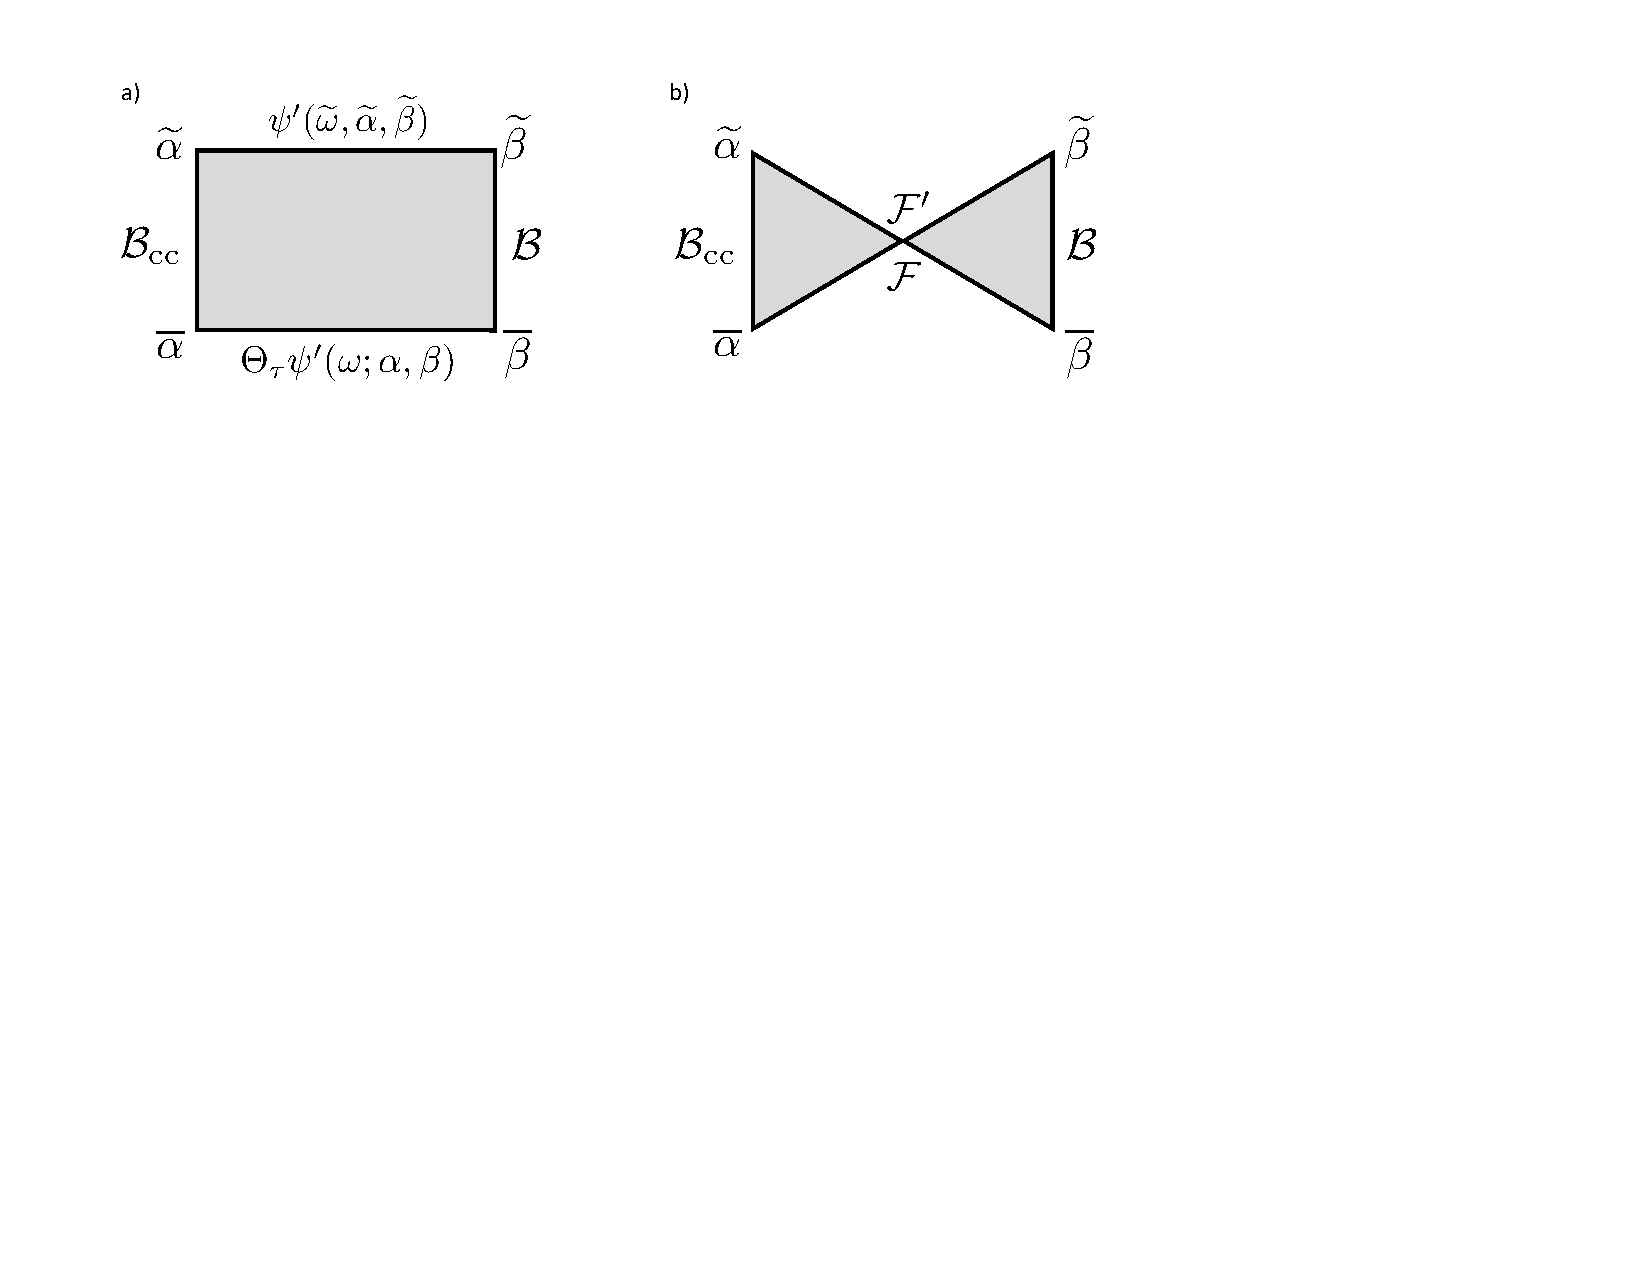
\includegraphics[width=0.86\textwidth]{figures/5.pdf}
 \caption{\small (a) 带所示边界条件的矩形上的路径积分可用于计算内积。(b) 矩形可约化为在顶点粘合的三角形之并。计算相应路径积分时，须对穿过该顶点传播的态求和。}
 \label{newrectangle}
\end{figure}

值得注意的一点是：与余切丛的讨论不同，态 $\psi'(w;\alpha,\beta)$ 可归一化。令 $w=\t w$ 时图 \ref{newrectangle} 不出现奇点。在当前背景下不应期待遇到 delta 函数态，因为例如 $M$ 紧时物理态空间有限维，不会有 delta 函数态这种东西。

\subsection{当 $Y$ 为超 Kähler 且 $M$ 紧时会发生什么}\label{hyperm}

在结束这个主题之前，我们不应忘记说明：在一个重要的特殊情形中，存在一种更简单的办法，可以部分地比较膜量子化与几何量子化。

在整个分析中，我们只是把 $Y$ 当作复辛流形。我们并未假设 $Y$ 的复辛结构能延拓为第 \ref{amo} 节所述意义下的完备超 Kähler 结构。这个假设足以保证 $Y$ 存在良好的 $A$-模型，并且它在许多有趣的例子中成立。但它很可能并非必需。

若我们确实假设 $Y$ 的复辛结构延拓为超 Kähler 结构，那么就会出现一种更简单的办法来部分比较膜量子化与几何量子化。这其实已在 \cite{GW}（第 2.3 与 4 节）中讨论过。首先，$Y$ 的对称 $\tau$ 在复结构 $I$ 中是反全纯的，但它在复结构 $J$ 中实际上是全纯的（见式 \eqref{tabush}）。因此 $M$ 作为不动点集的一个分支，在复结构 $J$ 中是全纯的。由于 $\omega_J$ 关于 $J$ 是 Kähler 的，这意味着复结构 $J$ 给出 $M$ 的一个复 Kähler 极化，即几何量子化意义下的极化。

用这个极化对 $M$ 作几何量子化，得到的 Hilbert 空间是
\be\label{hgq}\H_\gq=H^0(M,K_M^{1/2}\otimes\frL),\ee
其中照例 $\frL$ 是预量子线丛。（为简单起见，我们假设 $\frL$ 的 $\CP$ 曲率 $F=\omega_J$ 足够正，使高阶上同调消失。）Hilbert 空间结构由内积
\be\label{ngg}(\psi,\chi)=\int_M\d\mu\,\bar\psi\chi\ee
给出，其中 $\d\mu$ 是由辛结构 $\omega_J$ 导出的测度。

让我们看看能否为 $\H_\gq$ 与膜量子化所得之间建立关系。首先注意，在此情形中，$\B_\cc$ 与支撑在 $M$ 上的拉格朗日膜 $\B$ 都是 $(A,B,A)$ 型膜：它们关于辛结构 $\omega_I$ 与 $\omega_K$ 是 $A$-膜，关于复结构 $J$ 是 $B$-膜。这可如下看出。\footnote{作为 $\omega_I$、$\omega_K$ 的 $A$-模型以及 $J$ 的 $B$-模型的微分的超荷是线性相关的。因此只需检验其中两个微分下的不变性；第三个不变性随之成立。直接检验全部三个不变性似乎更有启发性，所以我们这样做。}

对 $\B$ 的情形，我们只需注意：由于 $\omega_I$ 是 $\tau$-奇的（式 \eqref{tabush}），$\tau$-不变子流形 $M$ 关于 $\omega_I$ 是拉格朗日的，正如它关于 $\omega_K$ 一样。因此 $\B$ 关于 $\omega_I$ 是 $A$-膜，正如它关于 $\omega_K$ 一样。另一方面，我们已经注意到 $M$ 在复结构 $J$ 中是复子流形。$\B$ 的 $\CP$ 丛满足 $\sF+\sB=0$。特别地，$\sF+\sB$ 在复结构 $J$ 中为 $(1,1)$ 型。支撑在复子流形上、且 $\sF+\sB$ 为 $(1,1)$ 型的膜是 $B$-膜，故 $\B$ 在复结构 $J$ 中是 $B$-膜。简言之，它是 $(A,B,A)$ 型膜。

对 $\B_\cc$，其支撑是整个 $Y$，而 $Y$ 在复结构 $J$ 中是复流形；其 $\CP$ 曲率满足 $\sF+\sB=\omega_J$，后者在复结构 $J$ 中为 $(1,1)$ 型。这些条件同样保证 $\B_\cc$ 关于 $J$ 是 $B$-膜。$\B_\cc$ 关于 $\omega_K$ 是 $A$-膜，因为 $\omega_K^{-1}(\sF+\sB)=I$ 是可积复结构；类似地，它关于 $\omega_I$ 是 $A$-膜，因为 $\omega_I^{-1}(\sF+\sB)=-K$ 是可积复结构。所以 $\B_\cc$ 同样是 $(A,B,A)$ 型膜。

对于 $M$ 的量子化，按我们通常的 $\CP$ 丛选择（$\B_\cc$ 取平凡丛，$\B$ 取 $\frL^{-1}$），膜量子化给出的答案是 $\omega_K$ 的 $A$-模型中 $(\B,\B_\cc)$ 弦的空间。我们一直简单地称之为 $\Hom(\B,\B_\cc)$，但在当前语境中最好写成
$\Hom_{A_K}(\B,\B_\cc)$，下标 $A_K$ 提醒我们考虑的是 $\omega_K$ 型 $A$-模型中的物理弦态。几何量子化用 Kähler 极化 $J$ 对 $M$ 量子化给出的答案 \eqref{hgq}，等同于 $\Hom_{B_J}(\B,\B_\cc)$，也就是复结构 $J$ 的 $B$-模型中 $(\B,\B_\cc)$ 弦的空间。

因此，用复结构 $Y$ 的膜量子化，与用复 Kähler 极化 $K$ 的几何量子化一致，当且仅当
$\Hom_{A_K}(\B,\B_\cc)$ 与 $\Hom_{B_J}(\B,\B_\cc)$ 重合。一般说来，这大概期望过高，尽管明确的反而例子并不显然。但正如 \cite{GW} 所指出的，若 $M$ 紧，则有一个非常简单的论证给出 $\Hom_{A_K}(\B,\B_\cc)$ 与 $\Hom_{B_J}(\B,\B_\cc)$ 作为向量空间的同构，忽略它们的 Hermite 内积。论证很简单：若 $M$ 紧，则不必考虑某个扭转拓扑场论中的 $(\B,\B_\cc)$ 弦空间，而可以直接考虑 $(\B,\B_\cc)$ 系统的超对称基态。作为向量空间，这与任何可能的扭转超对称场论中的物理态空间相同；这一观察蕴含向量空间 $\Hom_{A_K}(\B,\B_\cc)\cong\Hom_{B_J}(\B,\B_\cc)$ 的等价。

然而，这一关系并\emph{不}延拓为 Hermite 内积之间的关系。没有理由期望 $\Hom_{A_K}(\B,\B_\cc)$ 的 Hermite 内积与式 \eqref{ngg} 所描述的 $\H_\gq$ 的内积一致。至于 $\Hom_{B_J}(\B,\B_\cc)$，要使它带有自然的 Hermite 结构，$Y$ 应具有一个在复结构 $J$ 中反全纯作用的 $\Z_2$ 对称。这样的对称的存在并不能由我们的假设推出，故一般说来 $\Hom_{B_J}(\B,\B_\cc)$ 没有 Hermite 结构。

在第 \ref{branecp} 节中，我们解释了：当 $M$ 具有由 $Y$ 的全纯极化 $\varPi$ 诱导的复结构 $\J$ 时，$\Hom_{A_K}(\B,\B_\cc)$ 作为向量空间与 $H^0_\J(M,K_M^{1/2}\otimes\frL)$ 相同。这一描述确实附带了一个描述 $\Hom_{A_K}(\B,\B_\cc)$ 的 Hermite 内积的配方，但该配方相当不显式，涉及一个一般难以计算的全纯三角形。人们并不期望这个配方一般会化为几何量子化所建议的通常定义 \eqref{ngg} 那样简单的东西。

于是我们有两种策略，把通过复化 $Y$ 对 $M$ 的膜量子化，与用复 Kähler 极化的量子化相比较。一种策略使用 $Y$ 的全纯极化，另一种使用 $Y$ 的超 Kähler 结构。

与其进一步讨论本文分析过的那类初等例子，我们将在更精细的例子的背景下讨论这两种途径；这个例子曾从超 Kähler 观点在 \cite{GW} 第 4 节中讨论过（那里给出了比我们这里所说的更多细节）。

\subsection{平坦 $G$-丛模空间的量子化}\label{flatg}

设 $G$ 为紧 Lie 群，复化为 $G_\C$。记 $\g$ 与 $\g_\C$ 为相应的 Lie 代数。$G_\C$ 有反全纯对合 $\varrho$，其不动点集为 $G$。设 $C$ 为紧闭可定向二维流形，$M$ 为指定拓扑型的平坦 $G$-丛\footnote{本讨论中我们忽略 $M$ 的奇点带来的技术问题。例如，取 $G=\SO(3)$ 并要求丛 $E$ 满足 $w_2(E)\ne0$，即可完全避开这类问题。} $E\to C$ 的模空间。$M$ 有自然的辛结构 $\omega_0$，我们将其归一化，使最小非零周期为 $2\pi$。对 $G=\SU(N)$，它可由公式 \cite{ABott}
\be\label{defform}\omega_0=\frac{1}{4\pi}\int_C\Tr\,\delta A\wedge\delta A\ee
定义，其中 $\Tr$ 是在 $G$ 的基本 $N$ 维表示中取迹，$\delta A$ 表示 $E$ 上平坦联络的变分。周期条件意味着 $\omega_0$ 是线丛 $\L\to M$ 的曲率（该线丛生成 $M$ 的 Picard 群模挠）。人们希望用辛结构\footnote{稍后提到的 Chern--Simons 与 WZW 模型的“等级”，按通常定义并不是 $\kappa$。为简单起见设 $G$ 单连通，它是 $k=\kappa-h$，其中 $h$ 是 $G$ 的对偶 Coxeter 数。对单连通的 $G$，有 $K_M^{1/2}\sim\L^{-h}$。在某些处理中，自然地把 $\frL\otimes K_M^{1/2}$ 而非 $\frL$ 称为预量子线丛，公式也直接用 $k$ 而非 $\kappa$ 写出。}
$\omega=\kappa\omega_0$ 与预量子线丛 $\frL=\L^\kappa$ 来量子化 $M$，其中 $\kappa$ 为某个整数。假设 $\kappa>0$ 不失一般性，因为反转 $C$ 的定向会使 $\kappa$ 变号。

$M$ 是 $\R\times C$ 上规范群为 $G$ 的三维 Chern--Simons 规范理论的相空间，其中 $\R$ 参数化“时间”\cite{WittenJ}。量子化的目标是构造与空间流形 $C$ 相伴的 Hilbert 空间。$M$ 的辛结构只用到 $C$ 的定向，不用 $C$ 的其他结构。因此形式上可以希望，量子化能够以这样的方式进行，使 $M$ 的保定向微分同胚自然地作用在量子 Hilbert 空间上。事实上，若要从三维 Chern--Simons 理论得到拓扑场论，这一点是必需的。

对膜量子化而言，第一步是选取 $M$ 的一个好的复化。确实，$M$ 有好的复化 $Y$，即平坦 $G_\C$-丛 $\h E\to C$ 的模空间。它是复辛流形；复结构来自 $G_\C$ 的复结构，而全纯辛结构由公式 \eqref{defform} 把 $\g$-值平坦联络 $A$ 换成 $\g_\C$-值平坦联络 $\cA$ 来定义，是 $M$ 的辛结构的解析延拓。$Y$ 上典型的全纯函数，是 $\cA$ 沿 $C$ 中给定定向环的和乐在某个全纯表示中的迹。为与本文记号一致，我们称此复结构为 $I$；不过在 Hitchin 关于 Higgs 丛的工作 \cite{Hitchin}（其相关性稍后说明）以及该工作对几何 Langlands 的应用中，它通常被称为 $J$。$Y$ 有反全纯对合 $\tau$ 固定 $M$。$\tau$ 可通过把 $\varrho$ 作用在 $\cA$ 或其单值化上来定义。

$Y$ 的选择并未破坏 $C$ 的微分同胚对称性；$C$ 的保定向微分同胚作用在 $Y$ 上，并保持其复辛结构。因此形式上，膜量子化的程序给出 $M$ 量子化的微分同胚不变答案：它就是 $\H=\Hom_{A_K}(\B,\B_\cc)$。

我们可以通过选取全纯极化或选取超 Kähler 度量，试着把这一点具体化。（后一途径在 \cite{GW} 中有描述，其中某些细节比我们这里更详细。）两种途径都涉及一个看似破坏微分同胚对称性的辅助选择。但与 $\Hom_{A_K}(\B,\B_\cc)$ 的等价性表明，来自全纯极化或超 Kähler 度量的输出确实具有微分同胚对称性。

使 $M$ 的膜量子化更具体的两种途径，起点都是选取 $C$ 上的复结构。当然没有自然的选择；在连通到恒等的微分同胚之下，可能的选择构成 Teichmüller 空间 $\T$。对 $t\in\T$，记 $\I_t$ 为 $C$ 上相应的复结构。

给定 $\I_t$ 之后，就可以用 $Y$ 的全纯极化或超 Kähler 结构使膜量子化具体化。先描述全纯极化的途径。

给定 $\I_t$ 之后，平坦丛具有全纯结构（由平坦联络的 $(0,1)$ 部分定义）与反全纯结构（由 $(1,0)$ 部分定义）。为定义 $Y$ 的全纯极化，在 $Y$ 上放置一个等价关系：两个平坦 $G_\C$-丛若具有相同的全纯结构，就视为等价。$Y$ 中每点属于唯一的等价类。考虑包含平坦联络 $\cA=\d\bar z\cA_{\bar z}+\d z\cA_z$ 的等价类。同类中任何其他联络（模规范变换）有相同的 $(0,1)$ 部分，故形如
$\cA'=\cA+\W$，其中 $\W=\d z\W_z$ 是取值于 $\ad(\h E)$（$\h E$ 的伴随丛）的 $(1,0)$-形式。若 $\cA$ 平坦，则 $\cA'$ 也平坦的条件是 $\W$ 全纯，也就是说它取值于 $H^0(C,K_C\otimes\ad(\h E))$。指标定理表明该向量空间的维数为 $n=\frac12\dim_\C Y$。于是这些等价类是 $\C^n$ 的拷贝，此构造定义了 $Y$ 的全纯极化 $\varPi_t$。

可以这样看出 $\varPi_t$ 在 $M$ 上诱导出复极化。由 $\varPi_t$ 的定义，$M$ 的每点都含于唯一的叶；剩下的问题是证明每个叶至多含 $M$ 中的一个点。这一陈述是 Narasimhan--Seshadri 定理的一部分，该定理建立了 $C$ 上稳定全纯 $G_\C$-丛与平坦 $G$-丛之间的对应。交 $F\cap M$ 是给定全纯 $G_\C$-丛上平坦酉 $\g$-值联络的空间。Narasimhan--Seshadri 定理说，若 $E$ 稳定，则 $F\cap M$ 是单点；否则为空。

用复平坦联络的展开 $\cA=\cA_{\bar z}\d\bar z+\cA_z\d z$ 来看，叶空间由 $\cA_{\bar z}$ 全纯地参数化。限制到 $M$ 后，展开变为 $A=\d\bar zA_{\bar z}+\d zA_z$，其中 $A_z=-A_{\bar z}^\dagger$（这里假设约定为：酉平坦联络是反 Hermite 的）。因此 $\varPi$ 在 $M$ 上诱导的复结构，就是使 $A_{\bar z}$ 全纯变化的那一个。在此复结构（记作 $\J_t$）下，$M$ 可解释为 $C$ 上全纯 $G_\C$-丛的模空间。若写 $\delta A=\d z\delta A_z+\d\bar z\delta A_{\bar z}$，则公式 \eqref{defform} 关于 $\delta A_z$ 与 $\delta A_{\bar z}$ 是双线性的，这表明辛形式关于 $\J_t$ 为 $(1,1)$ 型，故 $\J_t$ 是 $M$ 的复极化。这与第 \ref{scbq} 节的一般论证相符。稍加小心便可证明，$\J_t$ 其实是 $M$ 的 Kähler 极化。

第 \ref{branecp} 节的论证适用于此例，它们表明膜量子化的 Hilbert 空间 $\H$ 作为向量空间就是
$\H=H^0_{\J_t}(M,K_M^{1/2}\otimes\frL)$。这一等价也附带一个不太显式的 $\H$ 的 Hilbert 空间结构描述，其中涉及一个全纯三角形。

把反全纯对合 $\tau$ 作用于 $\varPi_t$，得到另一个全纯极化 $\varPi'_t$。此极化的叶由具有相同反全纯结构的平坦 $G_\C$-丛组成。$\varPi'_t$ 在 $M$ 上诱导相反的复结构 $-\J_t$。一般地，如第 \ref{branecp} 节所解释，用复极化的几何量子化在复结构变号下不变。因此用 $\varPi'_t$ 的几何量子化给出与 $\varPi_t$ 等价的结果。我们将不再讨论 $\varPi'_t$。

使 $Y$ 的膜量子化具体化的另一条途径如下。一旦给二维流形 $C$ 指定复结构 $\I_t$，就可以表述并求解 Hitchin 方程 \cite{Hitchin}，使平坦 $G_\C$-丛 $\h E$ 具有 Higgs 丛的结构。空间 $Y$ 获得新的复结构 $J_t$，在其中它参数化 Higgs 丛；$Y$ 的复辛结构则延拓为超 Kähler 结构。（$J_t$ 在 Hitchin 的工作及后续大量文献中称为 $I$。）具体地说，Hitchin 方程涉及把 $\h E$ 的结构群从 $G_\C$ 约化到 $G$。相对于这一分解，复平坦联络 $\cA$ 分解为
$\cA=A+\i\phi$，其中 $A$ 是 $G_\C$-值平坦联络，$A=\d\bar zA_{\bar z}+\d zA_z$ 是 $G$-值联络，$\phi=\d\bar z\phi_{\bar z}+\d z\phi_z$ 是 $C$ 上伴随值的一形式。$A$ 与 $\phi$ 满足 Hitchin 方程。复结构 $J_t$ 就是使 $A_{\bar z}$ 与 $\phi_z$ 为全纯变量的那一个。

第 \ref{hyperm} 节的讨论表明，$\H$ 作为向量空间可等同于 $H^0_{J_t}(M,K_M^{1/2}\otimes\frL)$。但这一等同并不能给出 $\H$ 的 Hilbert 空间结构的描述。

解 Hitchin 方程得到的复结构 $J_t$ 定义在整个 $Y$ 上，而通过忘记平坦丛的反全纯结构得到的复结构 $\J_t$ 只定义在 $M$ 上。然而 $J_t$ 限制到 $M$ 时与 $\J_t$ 相同。为看出这一点，只需注意 $M$ 作为轨迹 $\phi=0$ 嵌入 $Y$。因此，使 $A_{\bar z}$ 与 $\phi_z$ 全纯的复结构 $J_t$，限制到 $M$ 上就是使 $A_{\bar z}$ 全纯的复结构 $\J_t$。

因此，由全纯极化得到的 $\H$ 描述，与解 Hitchin 方程得到的描述相同。

无论是全纯极化的描述，还是解 Hitchin 方程的描述，都没有说清 $H^0_{\J_t}(M,K_M^{1/2}\otimes\frL)$ 为何、或在何种意义下与 $t\in\T$ 的选择无关。然而这正是与膜量子化的关系所预言的。它也是三维 Chern--Simons 规范理论的拓扑不变性 \cite{WittenJ}，以及获得二维共形场论 WZW 模型的全纯分解的满意图像 \cite{KZ} 所需要的。通常的做法是把 $H^0_{\J_t}(M,K_M^{1/2}\otimes\frL)$ 视为 $\T$ 上某个向量丛的纤维，并在该向量丛上构造（投影）平坦联络。积分这个平坦联络，就给出不同 $t$ 的 $H^0_{\J_t}(M,K_M^{1/2}\otimes\frL)$ 之间的等价，从而恢复拓扑不变性，并在二维共形场论与三维拓扑场论中得到满意的结果。该平坦联络已从多个观点构造出来 \cite{ADW,Hitchtwo,Faltings}；不同途径被证明给出等价的结果 \cite{And}。这个平坦联络与 WZW 共形场论的共形块空间上的自然平坦联络一致 \cite{Las}。为与三维 Chern--Simons 规范理论的酉性以及二维 WZW 模型的预期性质相容，这个平坦联络必须是酉的；也就是说，它必须保持纤维上某个正 Hermite 内积。于是平坦联络的整体单值化给出映射类群的酉表示（更确切地说，是其中心扩张，因为该联络只是投影平坦的）。已知的规范论构造并没有给出像几何量子化所建议的公式 \eqref{ngg} 那样简单的东西。人们相信 \cite{El,Gaw,Gaw2}，正确的公式需要一个额外因子，其形式为
\be\label{nggo}(\psi,\chi)=\int_M\d\mu\,\bar\psi\chi\,e^{G_\kappa},\ee
其中 $e^{G_\kappa}$ 是靶为 $G_\C/G$、等级为 $\kappa$ 的 WZW 模型的配分函数。这个因子来自从所有联络的空间约化到平坦酉联络空间 $M$ 时，对 $G_\C$-值规范变换轨道的积分。抽象地，已经证明该平坦联络实际上是酉的 \cite{And2}；更具体地，已知酉结构可由诸如 \eqref{nggo} 的公式定义，其中当 $\kappa$ 很大时有渐近展开 $G_\kappa=F+\sum_{n=1}^\infty\kappa^{-n}F_n$，首项 $F$ 是 $M$ 的 Ricci 势 \cite{And3}。在首阶，这一结果与基于 $G_\C/G$ 的 WZW 模型的预言一致 \cite{And4}。

膜量子化给出的 Hilbert 空间内积答案，就是我们在第 \ref{branecp} 节描述的那个。这一描述不太显式，因为它依赖于一个难以计算的全纯三角形。理解预期因子 $e^{G_\kappa}$ 如何在这一途径中出现，将会极其有趣。

\subsection{$A$-膜与 $B$-膜}\label{flatcon}

这里我们将描述 $(B,A,A)$ 型膜的模空间的一些基本性质。除其他用途外，这将使我们更好地理解全纯极化在第 \ref{branecp} 节那样的论证中所起的作用。

首先考虑一个实辛流形 $S$ 的 $A$-模型，其辛形式为 $\omega$。秩 1 拉格朗日 $A$-膜 $\B$ 支撑在拉格朗日子流形 $L\subset S$ 上，并带有一个 $\CP$ 丛 $\L$，其联络 $\sA$ 与曲率 $\sF$ 满足 $\sF+\sB=0$。为形变 $\B$，一般可以同时形变 $L$ 与 $\sA$。$\sA$ 的一般形变具有形式 $\sA\to\sA+\veps\sa$，其中 $\sa$ 是一形式、$\veps$ 是小参数。为保持条件 $\sF+\sB=0$，要求 $\d\sa=0$。然而，若 $\sa$ 恰当，即 $\sa=\d\phi$（某个 $\phi$），则形变 $\sA\to\sA+\veps\sa$ 只是规范变换。因此非平凡形变由 de Rham 上同调 $H^1_{\dR}(L,\R)$ 给出。先假设 $L$ 紧。于是由 Hodge 理论，非平凡形变对应于调和一形式 $\sa$。

\begin{figure}[htbp]
 \centering
 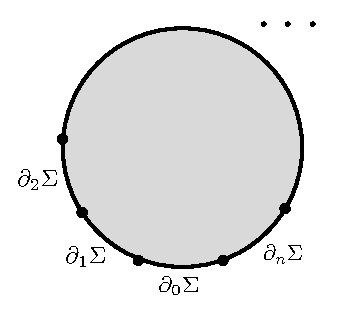
\includegraphics[width=0.42\textwidth]{figures/6.pdf}
 \caption{一个圆盘，其边界段依次标为 $\partial_0\Sigma$、$\partial_1\Sigma$、$\cdots$、$\partial_n\Sigma$。在每一段 $\partial_\alpha\Sigma$（$\alpha=0,1,\cdots,n$）上，边界条件由膜 $\B_\alpha$ 定义。顶点算符插入在各段之间的接点处。}\label{worldsheet}
\end{figure}

现在转而考虑 $L$ 的形变。局部可取坐标 $p_i,q^j$，使 $\omega=\sum_i\d p_i\d q^i$，且 $L$ 由 $p_1=\cdots=p_n=0$ 描述。任何一形式 $b=\sum_i b_i\d q^i$ 都给出 $L$ 的一个可能形变，其中方程 $p_i=0$ 被形变为 $p_i=\veps b_i$。这保持 $L$ 为拉格朗日子流形，当且仅当 $b$ 闭，即 $\d b=0$。然而，若 $b$ 恰当，$b=\d\rho$（某个函数 $\rho(q)$），则 $L$ 的形变由 $\rho$ 生成的 $M$ 的无穷小辛同胚给出，即
$\delta p_i=\{p_i,\rho\}=\partial\rho/\partial q^i$，
$\delta q_i=\{q_i,\rho\}=0$。用辛同胚对 $L$ 作形变，作为 $A$-膜 $\B$ 的形变是平凡的。稍后我们将明确演示这一点。因此在 $A$-模型中，$L$ 的非平凡形变在一阶对应于闭而非恰当的一形式，换言之对应于 de Rham 上同调 $H^1_{\dR}(L,\R)$。同样，若 $L$ 紧，这与调和一形式 $b$ 的空间相同。

比较上两段，我们看到 $\B$ 作为 $A$-膜的可能形变的模空间 $\M$ 上有一个明显的近复结构。在此近复结构中，$a+\i b$ 是 $(1,0)$ 型形变。事实上，这个近复结构可积，$\M$ 是复流形。

现在明确看看为什么一形式 $a$ 与 $b$ 中的恰当项代表 $\B$ 作为 $A$-膜的平凡形变。考虑定向二维流形 $\Sigma$ 上 $A$-模型的 $\sigma$-模型作用量，以及映射 $X:\Sigma\to M$。$\Sigma$ 的边界 $\partial\Sigma$ 是若干段 $\partial_\alpha\Sigma$ 的并，每段由带 $\CP$ 联络 $A_\alpha$ 的膜 $\B_\alpha$ 标记（图 \ref{worldsheet}）。设其中一段，比如 $\partial_0\Sigma$，由所关心的膜 $\B$ 标记，其 $\CP$ 联络为 $\sA$。在各段之间的接点处插入局部算符。设 $T$ 为这些接点的集合。$\sigma$-模型作用量的大部分是 $Q$-恰当的，其中 $Q$ 是通常的 $A$-模型微分。把非 $Q$-恰当的项写出，作用量可写成一般形式
\be\label{genformact} I=\int_\Sigma X^*(\omega)-\i\int_{\partial_0\Sigma}X^*(\sA)-\i\sum_{\alpha\ne0}\int_{\partial_\alpha\Sigma}X^*(\sA_\alpha)+\sum_{t\in T}c_t+\{Q,\cdots\}.\ee
非 $Q$-恰当的项是辛形式与 $\CP$ 联络的贡献，以及对应于接点处插入算符的可能端点贡献 $c_t$。$\partial_0\Sigma$ 的贡献在下文中很重要，故我们在 \eqref{genformact} 中把它单独分出。同样，重要的接点将是 $\partial_0\Sigma$ 的左右端点；我们称它们为 $t_r$ 与 $t_\ell$。若我们以 $a$ 或 $b$ 变分来形变膜 $\B$，即 $\delta\sA=a$，或 $\delta p_i=b_i,\ \delta q^j=0$，则作用量 $I$ 的改变是一个沿 $\partial_0\Sigma$ 的简单局部积分：
\be\label{varact}\delta I=-\i\int_{\partial_0\Sigma}(a_i+\i b_i)\d q^i.\ee
我们看到它自然地以组合 $a+\i b$ 依赖于 $a$ 与 $b$，这正是模空间 $\M$ 的复结构的表现。现在把它特殊化到我们将称为恰当变分的情形，即 $a+\i b=\d\nu$，其中 $\nu$ 是某个复值函数。此时积分化为边界项之和
\be\label{varacto}\delta I=-\i(\nu(t_r)-\nu(t_\ell))\ee
（我们简记 $\nu(X(t))$ 为 $\nu(t)$）。于是我们可以通过适当变换 $\partial_0\Sigma$ 端点处的插入来补偿恰当变分：
\be\label{endvar}\delta c_r=\i\nu(t_r),\quad\delta c_\ell=-\i\nu(t_\ell).\ee
最后，我们可以更精确地表述“由恰当形变联系的 $A$-膜等价”这一陈述。要断言 $\B$ 的恰当形变在某种意义下平凡，我们需要知道：在对 $\B$ 作恰当形变时，对于任何其他 $A$-膜 $\B'$，该如何处理 $\Hom(\B,\B')$ 与 $\Hom(\B',\B)$。式 \eqref{endvar} 回答了这个问题：它告诉我们，当对 $\B$ 作恰当形变以得到真正平凡的形变时，$\partial_0\Sigma$ 端点处的插入必须如何修改。

现在特殊化到辛流形 $S$ 实际上是复辛流形 $Y$、且 $\B$ 是 $(B,A,A)$ 型膜、支撑在复拉格朗日子流形 $L$ 上的情形。于是 $L$ 在某个复结构 $I$ 下是复流形，并且关于全纯辛形式 $\Omega=\omega_J+\i\omega_K$ 是拉格朗日的。为把 $\B$ 作为 $B$-膜形变，我们可以把 $L$ 作为复子流形形变，并把 $L$ 上的平坦 $\CP$ 丛 $\L$ 作为全纯线丛形变。$\B$ 的这两类形变都由复模参数化。若 $L$ 是紧 Kähler 流形，则无论把 $\B$ 视为 $I$ 型的 $B$-膜，还是视为关于 $\omega_J$ 或 $\omega_K$ 的 $A$-膜，参数化 $\B$ 形变的模空间 $\M$ 都相同。其理由本质上已在第 \ref{hyperm} 节解释：$\M$ 的切空间是 $(\B,\B)$ 系统的超对称基态空间，而后者可在物理 $\sigma$-模型层面定义，无需特殊化到某个扭转拓扑场论。然而，视我们把 $\M$ 视为复结构 $I$ 中 $B$-膜的模空间，还是视为辛结构 $\omega_J$ 或 $\omega_K$（或它们的线性组合）中 $A$-膜的模空间，$\M$ 具有不同的复结构。

在紧 Kähler 流形 $M$ 上，Hodge 分解把调和一形式表为 $(1,0)$ 型与 $(0,1)$ 型部分之和，给出展开 $a=a^{(1,0)}+a^{(0,1)}$、$b=b^{(1,0)}+b^{(0,1)}$。若把 $\M$ 视为参数化 $I$ 型 $B$-膜，则其复结构中的全纯方向由 $a^{(0,1)}$ 与 $b^{(1,0)}$ 参数化。若把它视为参数化关于辛结构 $\J_\zeta$ 的 $A$-膜，其中 $\J_\zeta$ 是 $\omega_J$ 与 $\omega_K$ 的线性组合，则全纯方向由
$a^{(0,1)}+\zeta b^{(0,1)}$ 与 $a^{(1,0)}-\zeta^{-1}b^{(0,1)}$ 参数化，其中 $\zeta$ 依赖于所考虑的线性组合（可选取约定使 $\zeta=1$ 对应 $\omega_J$、$\zeta=\i$ 对应 $\omega_K$）。当 $\zeta=0$ 时，$\J_\zeta$ 化为 $I$ 型 $B$-模型中适用的复结构；当 $\zeta=\infty$ 时，它化为相反的复结构，适用于 $-I$ 型 $B$-模型。

若 $L$ 不紧，则一般说来 $\B$ 作为 $B$-膜的模与作为 $A$-膜的模之间没有这种关系。与其一般地讨论，不如看看在我们的分析中实际重要的例子会怎样。这就是 $(B,A,A)$ 型膜 $\F$ 支撑在全纯极化 $\varPi$ 的一个叶 $F$ 上、且 $\CP$ 丛平凡的情形。由于 $F\cong\C^n$，$F$ 单连通，$\F$ 作为 $A$-膜实际上没有模。另一方面，$\F$ 作为 $B$-膜确有模，因为 $\varPi$ 的不同叶支撑不等价的 $B$-膜。局部可用全纯变量 $q^i$ 参数化叶的选择，用全纯变量 $p_i$ 参数化叶，使 $\Omega=\sum_i\d p_i\d q^i$。于是特定的叶由指定 $q^i$ 的值确定，比如 $q^i=w^i$。不同的 $w^i$ 选择标记不同的 $B$-膜；但粗略地说——稍后我们会给出更准确的说法——这些膜作为 $A$-膜全都相同。

“由给定 $\vec w=(w^1,w^2,\cdots,w^n)$ 标记的 $A$-膜 $\F$ 与 $\vec w$ 无关”这一断言可能显得费解，因为对 $\vec w$ 的依赖在我们的分析中其实很重要。关键在于，我们总是把膜 $\F$ 与 $\Hom(\B_\cc,\F)$ 中一个 distinguished 元素一起考虑，该元素对应于波函数 $\alpha=(\d\vec p)^{1/2}$。膜 $\F$ 连同 $\Hom(\B_\cc,\F)$ 的这个特定元素，确实非平凡地——而且正如我们将看到的，全纯地——依赖于 $\vec w$。要得到 $\F$ 的平凡变分，我们希望把 $\F$ 的改变与端点耦合 $c_\ell,c_r$ 的改变（如式 \eqref{endvar} 所示）配套。这与使用不依赖 $\vec w$ 的波函数 $\alpha=(\d\vec p)^{1/2}$ 不同。

让我们看看，当我们把膜 $\F$ 变到同一全纯极化的邻近叶，例如把 $w^i$ 平移某些复常数 $b^i$ 时，情形如何。回顾在量子化相关的情形中，复化辛形式为 $\omega_\C=-\i\Omega$，且 $\F$ 的 $\CP$ 丛平凡。作用量（见式 \eqref{genformact} 与 \eqref{toldo}）变为
\be\label{specformact} I=-\i\int_\Sigma X^*(\Omega)+c_\ell+c_r+\cdots+\{Q,\cdots\},\ee
其中我们省略了区间 $\partial_0\Sigma$ 之外的边界项与耦合，因为它们不受我们即将所作的形变影响。为描述通过改变 $\vec w$ 对膜 $\F$ 所作的改变，我们在 $\partial_0\Sigma$ 附近变分映射 $X$：$\delta p_i=0$、$\delta q^i=b^i$。由 $\Omega=\sum_i\d p_i\d q^i$，得到
\be\label{acttrans}\delta I=\i\int_{\partial_0\Sigma}b^i\d p_i=\i b^i p_i(t_r)-\i b^i p_i(t_\ell).\ee
于是为得到真正平凡的形变，补偿性的端点变分为
\be\label{nactra}\delta c_r=\i b^i p_i(t_r),\quad\delta c_\ell=-\i b^i p_i(t_\ell).\ee

我们可以如下解释这些结果。首先，$\F$ 的这个变分是全纯的，因为作用量的变分正比于 $\delta w^i=b^i$，而不含正比于 $\delta\bar{w^i}=\bar{b^i}$ 的项。这证实了第 \ref{branecp} 节中的断言。其次，为补偿 $\F$ 的位移所需的特定变分 $\delta c_\ell$、$\delta c_r$，可以直观地理解如下。$\F$ 的位移由 $b^i\frac{\partial}{\partial q^i}$ 给出，它生成 $q^i\to q^i+b^i$。量子力学上，$b^i\frac{\partial}{\partial q^i}$ 对应于 $\i b^i p_i$。对于表示 $\Hom(\B',\F)$ 或 $\Hom(\F,\B')$（$\B'$ 为某个其他膜）中元素的顶点算符，其修正涉及乘以 $\pm\i b^i p_i$。

$b^i p_i$ 如何作用在 $\Hom(\B',\F)$ 或 $\Hom(\F,\B')$ 上，取决于所考虑的膜的类型。设 $\B'=\B_\cc$。则 $\Hom(\B_\cc,\F)$ 与 $\Hom(\F,\B_\cc)$ 等同于 $H^0(F,K_F^{1/2})$。一般元素形如 $f(\vec p)(\d\vec p)^{1/2}$，而 $b^i p_i$ 作为乘法算符作用。另一方面，设 $\B'$ 是拉格朗日 $A$-膜，其支撑 $L$ 与 $F$ 交于单点 $w$。则作用在 $\Hom(\F,\B')$ 或 $\Hom(\B',\F)$ 上时，$p_i$ 可用其在 $w$ 处的值代替。

最后，考虑当我们变分全纯极化 $\varPi$ 的叶时会发生什么。$\varPi$ 的邻近叶等价，条件是我们按 $\delta q^i=b^i$ 改变叶时，如上所述用 $\pm\i b^i p_i$ 变换 $\Hom(\F,\B')$ 与 $\Hom(\B',\F)$。这可以看作由 $W$ 参数化的膜族上的平坦联络。但它是不可积的平坦联络。为积分这个平坦联络，我们必须把作用在 $\F$ 与其他膜之间角上的算符 $\pm\i b^i p_i$ 取指数。例如，要断言 $q^i$ 相差非无穷小平移 $b^i$ 的两个纤维等价，我们必须把它们与 $\B_\cc$ 的角乘以 $\exp(\pm\i\sum_i b^i p_i)$。这样的指数函数是不允许的；我们只允许 $p$ 的多项式函数。无法积分这个平坦联络是一个特性，而不是缺陷。在我们的应用中，断言 $\varPi$ 的不同纤维等价并不自然。

\section{对称性与对应}\label{symq}

\subsection{概览}\label{oversym}

如第 \ref{problem} 节所解释，对于带预量子线丛 $\frL$ 的实辛流形 $M$，不可能以这样的方式量子化：使经典力学的自然对称群 $\G$ 实现为量子 Hilbert 空间 $\H$ 上的酉变换群。（回忆 $\G$ 的元素是辛同胚 $\varphi:M\to M$ 连同 $\varphi$ 到 $\frL$ 的对称的提升。）既然如此，我们不如问如下问题：对于给定的量子化方法，$\G$ 的哪个子群在量子力学上实现为酉对称群？

在几何量子化中，这个问题有标准答案。$M$ 的几何量子化依赖于 $M$ 的极化 $\P$ 的选择。对给定的 $\P$，在量子力学上实现为对称群的 $\G$ 的子群，是保持 $\P$ 的子群 $\G_\P$。在有时重要的特殊情形中，几何量子化定义的 Hilbert 空间 $\H$ 容许 $\G$ 的更大子群以酉方式作用；但几何量子化的一般答案是，在量子理论中起作用的经典对称子群是 $\G_\P$。

例如，若 $M=T^*N$ 是带标准辛结构的余切丛，$\P$ 是叶为余切丛纤维的实极化，则我们可以相当显式地描述 $\G_\P$。保持 $\P$ 不变的辛同胚群 $\G_\P$ 由两类辛同胚生成。第一，$N$ 的每个微分同胚都延拓为 $T^*N$ 的保持辛结构的微分同胚。这些微分同胚置换 $\P$ 的叶。此外，还有把每个叶映到自身的 $T^*N$ 的辛同胚。若 $q^i$ 是 $N$ 上的局部坐标，$p_i$ 是余切丛纤维上相应的线性函数，则把每个叶映到自身的辛同胚保持 $q^i$ 不变，并把 $p_j$ 平移为
$p_j\to p_j+\partial f/\partial q^j$，
其中 $f(q^1,q^2,\cdots,q^n)$ 是某个函数（称为正则变换的生成函数）。

膜量子化中的对称群是什么？在膜量子化中，第一步是把带辛形式 $\omega$ 的实辛流形 $M$ 复化为带全纯辛形式 $\Omega$ 的复辛流形 $Y$。$Y$ 必须使得：若把 $Y$ 视为带辛形式 $\Im\Omega$ 的实辛流形，则其 $A$-模型良定义。（例如，$Y$ 可以是完备超 Kähler 流形，如第 \ref{amo} 节所讨论。）选定合适的 $Y$ 后，定义带 $\CP$ 丛 $\L$ 的拉格朗日膜 $\B$，则膜量子化的量子 Hilbert 空间为 $\H=\Hom(\B,\B_\cc)$。

对膜量子化的对称群，有一个显然的候选答案。$Y$ 的 $A$-模型的自然对称，是保持辛形式 $\Omega$ 的 $Y$ 到自身的可逆全纯映射，即全纯辛同胚。若 $Y$ 的全纯辛同胚把 $M$ 映到自身，且其在 $M$ 上的作用提升为对 $\frL$ 的作用，则它可能是膜 $\B$ 的对称。这给出膜量子化对称的自然候选。设 $\G_Y$ 为 $\G$ 中这样的元素构成的子群：其在 $M$ 上的作用可解析延拓为 $Y$ 的全纯辛同胚。则 $\G_Y$ 是酉作用于 $\H=\Hom(\B,\B_\cc)$ 的 $\G$ 的子群的自然候选。

尽管这个提法可能是正确的，要证明它实际上有技术困难。为使 $A$-模型具体化，通常要在 $Y$ 上选取 Riemann 度量 $g$。这可以是第 \ref{amo} 节所讨论的完备超 Kähler 度量。至少，$g$ 应与实辛形式 $\omega_K=\Im\Omega$ 一起定义一个近复结构 $K$，使 $\omega_K$ 为 $(1,1)$ 型且正。此外，$g$ 应使 $Y$ 的 $A$-模型真正存在。只要 $g$ 在使 $A$-模型存在的容许度量类中变化，$Y$ 的 $A$-模型就与 $g$ 无关。遗憾的是，最后这个条件很难处理，其全部含义也不易理解。

现在设 $\varphi$ 是 $Y$ 的全纯辛同胚。一般说来 $g$ 不是 $\varphi$-不变的，而会被 $\varphi$ 变成另一个度量 $g^\varphi$。带度量 $g^\varphi$ 的 $Y$ 的 $A$-模型一般可能并不良定义。即使良定义，要论证 $g$ 与 $g^\varphi$ 给出等价的 $Y$ 的 $A$-模型，我们也需要知道可以在容许度量类中把 $g$ 与 $g^\varphi$ 插值。总可以用一族与合适近复结构相伴的度量在 $g$ 与 $g^\varphi$ 之间插值。\footnote{其论证与稍后关于超 Kähler 度量的一个论证类似。$Y$ 的辛结构 $\omega_Y$ 把 $Y$ 切丛的结构群从 $\GL(4n,\R)$ 约化到 $\Sp(4n,\R)$。使 $\omega_Y$ 为正且为 $(1,1)$ 型的度量，对应于把结构群进一步约化到 $\Sp(4n,\R)$ 的极大紧子群 $\UU(2n)$。可以在任意两个这样的约化之间插值，因为商 $\Sp(4n,\R)/\UU(2n)$ 可缩。}但并不显然这种插值能在使 $A$-模型存在的度量类中进行。

物理上，人们更愿意把 $A$-模型看作紫外完备的 $\sigma$-模型的扭转版本。试图考虑基于诸如 $g^\varphi$ 的度量的 $A$-模型，一般会把我们带出那个世界；而基于从 $g$ 到 $g^\varphi$ 插值的论证可能把我们带得更远。

为进一步给读者定位，我们将描述一些具体问题，说明这个问题在何处成问题、在何处不成问题。然后我们将描述另一种途径，使人们能在紫外完备的世界中研究辛同胚。

我们将在 $M=\R^{2n}$ 的量子化背景下说明这个故事的两个方面，其中实值坐标为 $\vec x=(x^1,x^2,\cdots,x^{2n})$，标准辛结构为 $\omega=\frac12\sum_{i,j=1}^{2n}\omega_{ij}\d x^i\d x^j$。首先，我们试着用膜量子化解释标准结果\footnote{这也可由第 \ref{comparing} 节的论证推出：$\R^{2n}$ 的膜量子化不依赖于极化的选择，等价于用实线性极化的 $\R^{2n}$ 的几何量子化。}：$M$ 的量子化可以选为在仿射线性辛同胚群 $\vec x\to A\vec x+\vec b$ 下不变，如第 \ref{problem} 节所讨论。我们以熟悉的方式开始，把 $M$ 复化为复辛流形 $Y=\C^{2n}$，此时 $x^i$ 是 $Y$ 上的全纯坐标。$Y$ 的复结构与复辛结构当然是平移不变的，即在 $\vec x\to\vec x+\vec b$（$\vec b$ 为复常数）下不变。按第 \ref{amo} 节的意义，$Y$ 的平移不变复辛结构可通过选取合适的平移不变 Riemann 度量 $g$ 延拓为平移不变超 Kähler 结构。这样的 $g$ 构成的空间可如下描述。由于假设了平移不变性，我们可在一点 $y\in Y$ 处作分析。$Y$ 在 $y$ 处的切空间维数为 $4n$，故其线性变换群是 $\GL(4n,\R)$ 的一个拷贝。$Y$ 的复辛结构在子群 $\Sp(2n,\C)\subset\GL(4n,\R)$ 下不变。延拓其复辛结构的 $Y$ 上平移不变超 Kähler 度量，不在 $\Sp(2n,\C)$ 下不变，而在其极大紧子群下不变。这样的子群同构于辛群的紧实形式，我们称之为 $\Sp_c(2n)$。$\Sp(2n,\C)$ 的任一 $\Sp_c(2n)$ 子群都是被某个超 Kähler 度量保持的子群，且所有这样的子群在 $\Sp(2n,\C)$ 中共轭。因此，延拓 $Y$ 的复辛结构的平移不变超 Kähler 度量的空间是齐性空间 $\sW=\Sp(2n,\C)/\Sp_c(2n)$ 的一个拷贝。由 $\sW$ 参数化的任何超 Kähler 度量都可用于定义 $Y$ 的 $A$-模型。$\sW$ 可缩，特别地连通且单连通。故可在 $\sW$ 中任意两点 $w_1,w_2\in\sW$ 之间插值，而且这一插值在同伦意义下唯一。（唯一性很重要，因为从 $w_1$ 到 $w_2$ 的同伦不同的插值可能导致相差一个酉变换的量子理论之间的等价。）因此，若我们用平移不变超 Kähler 度量定义 $Y$ 的 $A$-模型，用哪一个并无关系。

现在我们可以用新的方式理解为什么 $M$ 的膜量子化在 $M$ 的仿射线性变换下不变。$M$ 的仿射线性辛同胚 $\vec x\to A\vec x+\vec b$ 可解析延拓为 $Y$ 的全纯辛同胚，由同一公式定义。一般的仿射线性辛同胚不会保持用于定义 $Y$ 的 $A$-模型的平移不变超 Kähler 度量。但它会把这个平移不变超 Kähler 度量变成另一个平移不变超 Kähler 度量，而 $Y$ 的 $A$-模型并不在乎我们用哪一个平移不变超 Kähler 度量。因此，通过 $A$-模型的 $M$ 的量子化在仿射线性辛同胚下不变；仿射线性辛同胚群作用在量子 Hilbert 空间 $\H$ 上。

为看出这类论证的局限，我们注意以下事实。$M=\R^{2n}$ 的、能延拓为 $Y$ 的全纯辛同胚的辛同胚群，比仿射线性辛同胚群大得多。在本讨论中，我们只考虑多项式辛同胚，因为我们在 $A$-模型中只允许多项式函数。为构造一个非常大的多项式辛同胚群，先把变量 $x^1,\dots,x^{2n}$ 分成 Poisson 交换的坐标 $q^1,\cdots,q^n$ 与共轭动量 $p_1,\cdots,p_n$。对任何多项式函数 $f(q^1,\cdots,q^n)$，考虑把 $p_i,q^j$ 映为
\begin{align}\label{worfo} p'_i&=p_i+\frac{\partial f}{\partial q^i},\cr q^i{}'&=q^i \end{align}
的辛同胚。这类辛同胚连同线性辛同胚\footnote{\label{enough}这里考虑线性辛同胚 $\vec x\to A\vec x$ 就足够了，不必考虑仿射线性辛同胚 $\vec x\to A\vec x+\vec b$，因为 $p$ 的常数平移已包含在式 \eqref{worfo} 中；而一旦包含线性辛同胚（它们可以交换 $p$ 与 $q$），$q$ 的常数平移也就包含在内了。}生成一个称为 $\R^{2n}$ 的驯顺辛同胚群的群。我们记之为 $\TAut(\R^{2n})$。为看出 $\TAut(\R^{2n})$ 有多么巨大，可以想象试着给这个群配一个 Lie 代数。（在这个无穷维情形中，这在技术上有问题。）这样的 Lie 代数将不得不把所有 $p$ 与 $q$ 的多项式函数作为生成元包含进来。确实，式 \eqref{worfo} 中的变换以 $f(q^1,\cdots,q^n)$ 为生成元。由于 $\TAut(\R^{2n})$ 包含线性辛同胚，而后者特别可以交换 $p$ 与 $q$，一个以任意多项式函数为生成元的假想 Lie 代数也必须包含 $p$ 的任意多项式函数。但这样一来，要得到在 Poisson 括号下封闭的函数类，我们就必须允许 $p$ 与 $q$ 的任意多项式。所以 $\TAut(\R^{2n})$ 大到这样的程度：若它能被当作 Lie 群处理，其 Lie 代数将包含正则变量的一切多项式。

对 $n=1$，已知 $\TAut(\R^{2n})$ 与 $\R^{2n}$ 的全体多项式辛同胚群 $\Aut(\R^{2n})$ 重合。对 $n>1$ 是否如此尚不清楚。（注意在 Lie 代数层面，人们看不出 $\TAut(\R^{2n})$ 与 $\Aut(\R^{2n})$ 的区别，因为如上所述，$\TAut(\R^{2n})$ 的 Lie 代数必须具有任意多项式生成元。）

在形变量子化中，我们可以考虑 $\C^{2n}$ 的一切全纯多项式辛同胚群 $\Aut(\C^{2n})$，以代替 $\Aut(\R^{2n})$。同样，我们可以考虑相应的驯顺子群 $\TAut(\C^{2n})$，以代替 $\TAut(\R^{2n})$；它由 $\vec x\to A\vec x+\vec b$ 连同式 \eqref{worfo} 中的辛同胚生成，只不过现在 $A$、$\vec b$ 与 $f$ 都可以是复的。这些群是 $\C^{2n}$ 上多项式函数经典环 $\A_0$ 及其 Poisson 括号的对称群。形变量子化把 $\A_0$ 换成非交换环 $\A$，有时称为 Weyl 代数（由生成元 $x_i$ 及关系 $[x_i,x_j]=\i\hbar\Omega_{ij}$ 定义）。经典对称群 $\TAut(\C^{2n})$ 与 $\Aut(\C^{2n})$ 的量子类比，是 $\A$ 的自同构群。$\TAut(\C^{2n})$ 与 $\Aut(\C^{2n})$ 同其量子类比有什么关系？

Kanel-Belov 与 Kontsevich \cite{BKK} 建立了惊人的结果：$\TAut(\C^{2n})$ 是 Weyl 代数自同构群的子群；他们并猜想，可能更大的群 $\Aut(\C^{2n})$ 就是 Weyl 代数的自同构群。这后来由 Kanel-Belov、Elishev 与 Yu \cite{BEY} 证明。（这些证明大量使用模素数 $p$ 约化；Weyl 代数在这样的约化后具有相当不寻常的性质。）正如第 \ref{symmeq} 节末尾将解释的，\cite{BKK,BEY} 的结果对 $\R^{2n}$ 的量子化（而非 $\C^{2n}$ 的形变量子化）有直接的类比。特别地，$\Aut(\R^{2n})$ 的中心扩张作为酉对称群作用在量子化 $\R^{2n}$ 所得的 Hilbert 空间上。这里没有量子形变。一方面，我们可能预期如此，因为这个中心扩张正是本讨论开头引入的群 $\G_Y$。另一方面，这个结果很引人注目，因为在 Lie 代数层面没有类似的东西成立。如前面所解释，$\Aut(\R^{2n})$ 甚至 $\TAut(\R^{2n})$ 的 Lie 代数将不得不包含 $\R^{2n}$ 上的一切多项式函数。由于从经典力学过渡到量子力学时通常的反常（第 \ref{problem} 节与附录 \ref{anomaly} 讨论过），这样的 Lie 代数无法在没有量子形变的情况下作用在量子 Hilbert 空间上。

用膜量子化恢复 \cite{BKK,BEY} 的部分结果是合理的目标。然而，$Y$ 的一般多项式辛同胚 $\varphi$ 会把 $Y$ 上的平移不变度量 $g$ 变成远离平移不变的度量 $g^\varphi$。一般说来，$g^\varphi$ 可能不给出紫外完备的 $\sigma$-模型；即使给出，我们也不知道如何在导致这类模型的 $Y$ 的度量类中于 $g$ 与 $g^\varphi$ 之间插值。因此，要从膜量子化恢复 \cite{BKK,BEY} 的部分结果，需要另一种途径。在第 \ref{corresp} 节中，我们将引入一种途径，使我们能在留在紫外完备世界的同时研究一般多项式辛同胚。这一途径的另一优点是，它为研究比辛同胚更一般的算符提供了良好的框架。

\subsection{界面与算符}\label{corresp}

辛流形 $Y$ 的辛同胚 $\varphi$ 是保持 $Y$ 的辛结构 $\omega$ 的可逆映射 $\varphi:Y\to Y$，即 $\varphi^*(\omega)=\omega$。具体地说，若 $x^i$ 是 $Y$ 上的局部坐标，则 $\varphi$ 可由把 $x'{}^{i}=\varphi^*(x^i)$ 表为 $x^k$ 的函数来定义：

\be\label{expfn} x'{}^{i}=f^i(x^k).\ee
说 $\varphi$ 可逆，是指这些关系可以反解，
\be\label{nexpfn} x^i=k^i(x'{}^{k}).\ee
$\varphi$ 是 $Y$ 的辛同胚（而不只是微分同胚）这一条件，意味着 $\varphi^*(\omega)=\omega$，更详细地说
\be\label{nexo}\sum_{i,j}\omega_{ij}(x')\d x'{}^{i}\d x'{}^{j}=\sum_{i,j}\omega_{ij}(x)\d x^i\d x^j.\ee
当然还可以加更多条件。若 $Y$ 是复流形且 $\varphi$ 是全纯映射，则可取 $x^i$ 为局部全纯坐标，此时函数 $f^i$ 与 $k^i$ 全纯。若 $Y$ 上有一个 distinguished 的多项式函数类，则当 $f^i$ 与 $k^i$ 为多项式时，$\varphi$ 是多项式映射。

辛同胚的条件 \eqref{nexo} 有一个有趣的解释。考虑 $Y$ 的两个拷贝之积，比如 $Y\times Y'$，其中 $x^i$ 视为 $Y$ 上的坐标，$x^{i'}$ 视为 $Y'$ 上的坐标。条件 $x'{}^{i}=f^i(x^k)$，或等价地 $x^i=k^i(x'{}^{k})$，定义了中间维子流形 $L\subset Y\times Y'$。把 $Y\times Y'$ 视为带辛结构 $\omega\boxplus(-\omega)$ 的辛流形，即 $Y\times Y'$ 的辛形式是第一个因子上 $\omega$ 与第二个因子上 $-\omega$ 之和。\footnote{\label{boxes}更详细地说，若 $\pi:\h Y\to Y$ 与 $\pi':\h Y\to Y'$ 是 $\h Y=Y\times Y'$ 到两个因子的投影，$\alpha,\alpha'$ 分别是 $Y$ 与 $Y'$ 上的二形式，则定义
$\alpha\boxplus\alpha'=\pi^*(\alpha)+{\pi'}^*(\alpha')$。类似地，若 $\RR,\RR'$ 是两个因子上的线丛，则定义 $\RR\boxtimes\RR'=\pi^*(\RR)\otimes\pi'^*(\RR')$。这是 $\h Y$ 上的线丛，在第一个因子上为 $\RR$、在第二个因子上为 $\RR'$。}
式 \eqref{nexo} 意味着 $L$ 是这个实辛结构下 $Y\times Y'$ 的拉格朗日子流形。

一般地，考虑两个辛流形 $Y,Y'$ 的积 $Y\times Y'$。$Y\times Y'$ 的拉格朗日子流形 $L$ 称为 $Y$ 与 $Y'$ 之间的拉格朗日对应。若拉格朗日对应 $L$ 如上所述与 $Y,Y'$ 间的某个辛同胚相伴，则它是非常特殊的情形：若 $y_0,y_0'$ 分别是 $Y$ 与 $Y'$ 中的点，则 $L$ 与 $y_0\times Y'$ 或 $Y\times y_0'$ 的交是单点。

\begin{figure}[htbp]
 \centering
 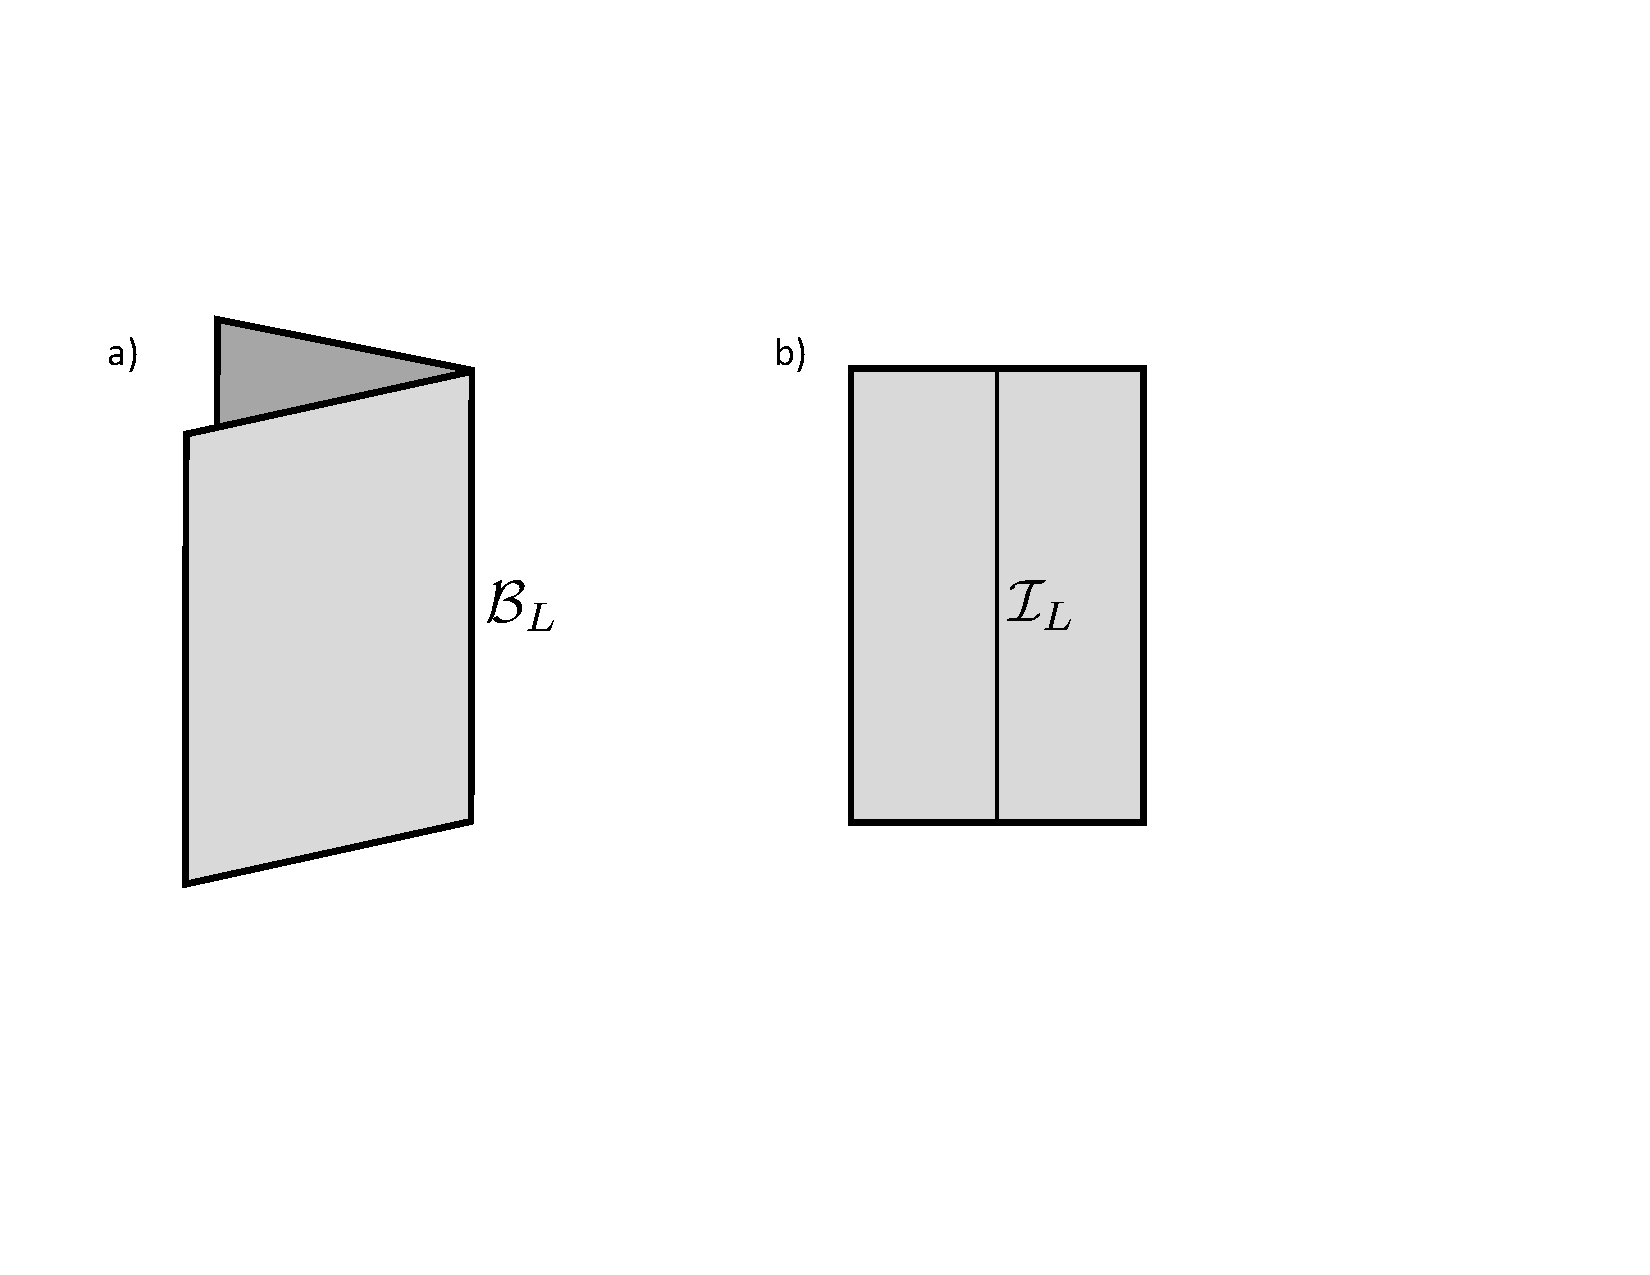
\includegraphics[width=0.72\textwidth]{figures/Folding.pdf}
 \caption{积 $Y\times Y'$ 的 $\sigma$-模型可理解为二维流形 $\Sigma$ 上的量子场，$\Sigma$ 有两张相同的叶，一张映到 $Y$、一张映到 $Y'$。(a) 我们考虑两叶仅通过一个与膜 $\B_L$ 相伴的边界条件耦合的情形。我们把这种耦合画成两叶沿边界粘合。(b) “展开”后，该膜成为靶为 $Y$（图左部）与 $Y'$（图右部）的 $\sigma$-模型之间的界面或畴壁 $\I_L$。$\I_L$ 支撑在中央竖线 $\ell$ 上。}\label{unfolding}
\end{figure}

若 $L$ 是 $Y\times Y'$ 中的拉格朗日对应，则在 $L$ 上选取平坦 $\spinc$ 结构后，可定义 $Y\times Y'$ 的 $A$-模型中的拉格朗日 $A$-膜 $\B_L$。在映射 $\Phi:\Sigma\to Y\times Y'$ 的 $\sigma$-模型中（$\Sigma$ 为二维流形），膜 $\B_L$ 的作用是沿 $\Sigma$ 边界的一部分 $\partial_0\Sigma$ 定义一个可能的边界条件。由于 $Y\times Y'$ 是简单乘积，可把 $\Sigma$ 想成有两张叶，一张映到 $Y$、一张映到 $Y'$；两叶仅沿 $\Sigma$ 的边界耦合。边界条件意味着 $\Phi$ 把 $\partial_0\Sigma$ 映到 $L\subset Y\times Y'$（边界耦合依赖于 $L$ 的 $\spinc$ 结构）。这一构造有一个有用的“展开”版本（图 \ref{unfolding}）。为此，我们沿 $\partial_0\Sigma$ 把 $\Sigma$ 的一张叶“翻过来”或展开。展开后，$\Sigma$ 被替换为二维流形 $\h\Sigma$，其中 $\partial_0\Sigma$ 不再是边界，而是内线 $\ell$。在 $\ell$ 的“左”边，$\Sigma$ 映到 $Y$；在右边，映到 $Y'$。于是在展开后的图像中，膜 $\B_L$ 被替换为 $Y$ 的 $\sigma$-模型与 $Y'$ 的 $\sigma$-模型之间的畴壁或“界面” $\I_L$。

到目前为止，这些是关于二维场论的一般论述。现在特殊化到 $Y'$ 是 $Y$ 的第二个拷贝、且我们研究的是 $Y'$ 上辛形式与 $Y$ 上辛形式反号的 $A$-模型的情形。“展开”反转 $\Sigma$ 的一张叶的定向；在 $A$-模型中，反转世界面定向等价于反转辛形式的符号。由于我们从两个 $Y$ 拷贝上相反的辛结构出发，展开后辛结构处处相同，我们就简单地得到单个 $Y$ 拷贝的普通 $A$-模型。先前图像中 $Y\times Y'$ 的 $A$-模型里的 $A$-膜 $\B_L$，展开后变成 $Y$ 的 $A$-模型中的拓扑畴壁或界面 $\I_L$。称此界面为“拓扑的”，意思是它可以在 $\Sigma$ 中自由移动而不影响 $A$-模型的可观测量。\footnote{特别地，可以把拓扑界面上移到边界，在那里它与已有边界条件结合成新的边界条件。这定义了数学语言中可称为边界条件范畴上的函子的东西。这在某些应用（包括几何 Langlands）中很重要；但这里我们将用拓扑界面定义普通的量子算符。}

\begin{figure}[htbp]
 \centering
 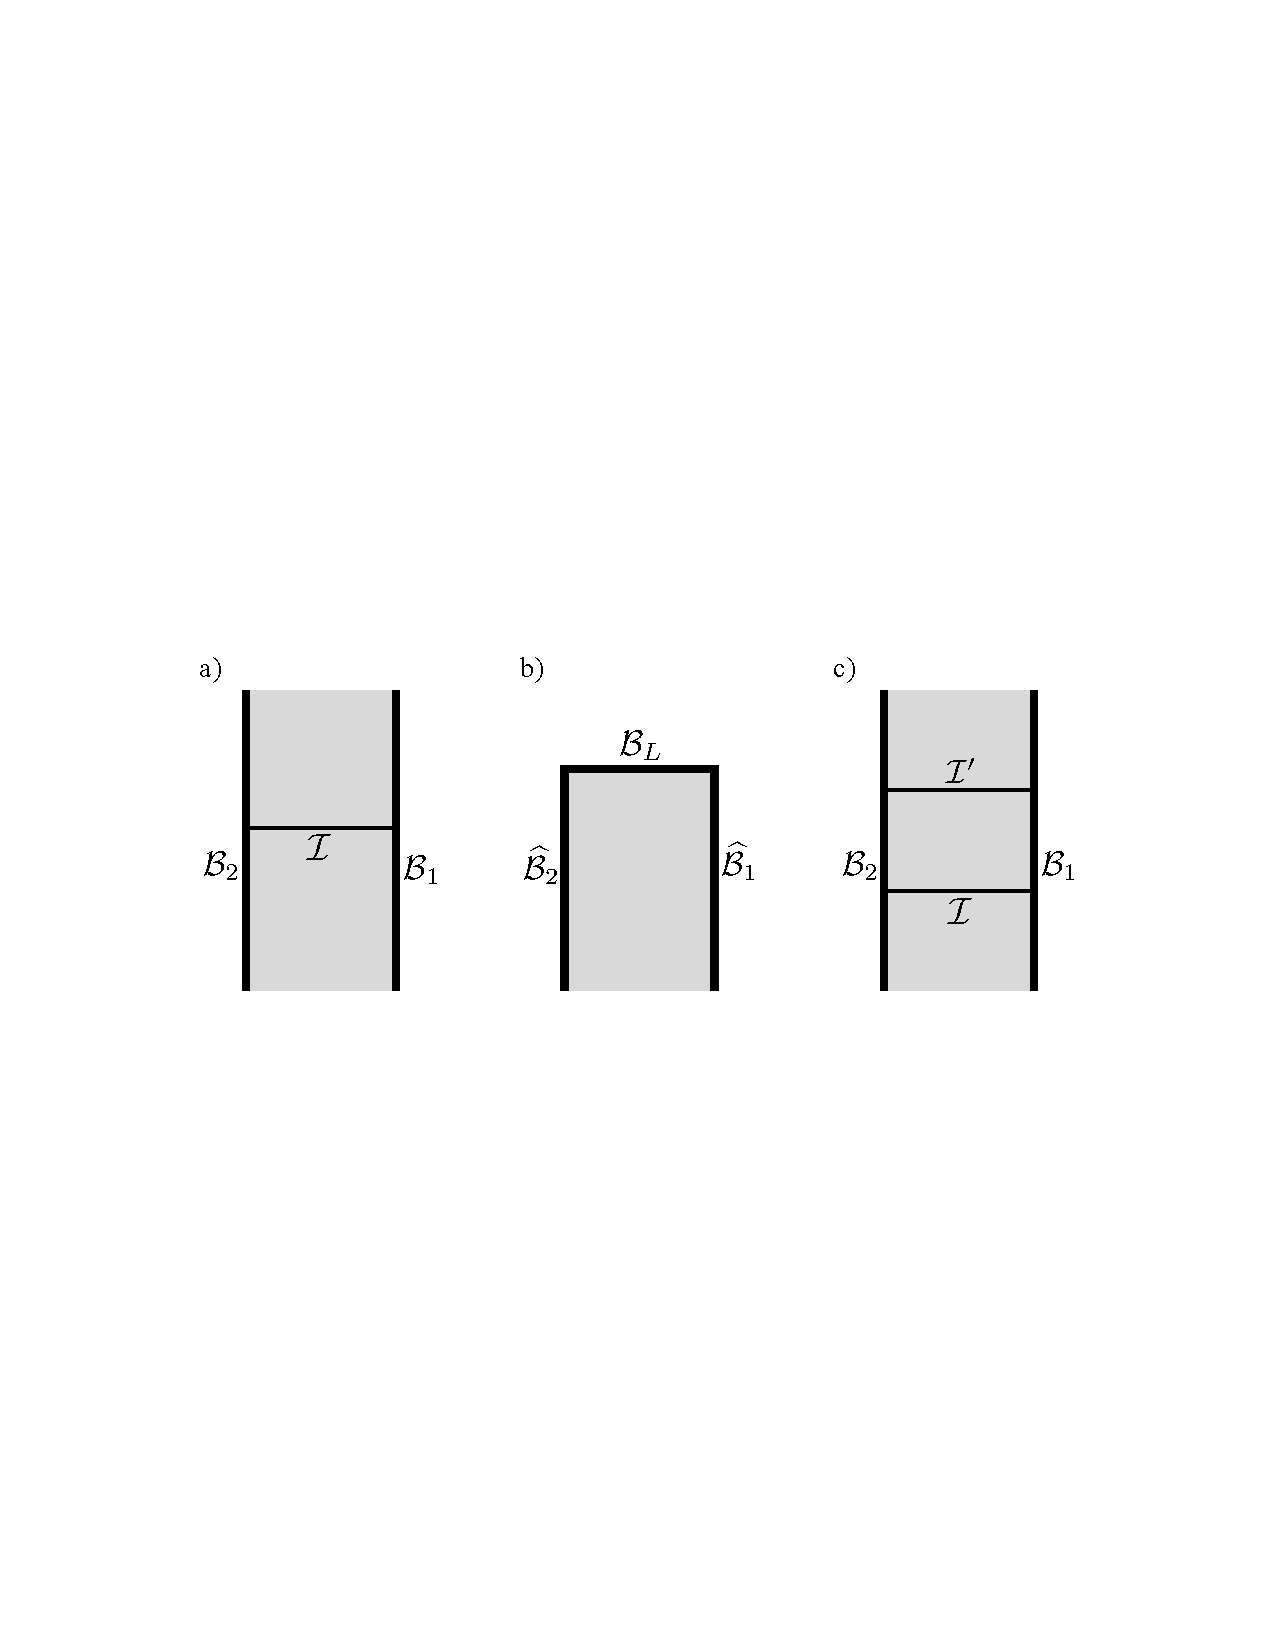
\includegraphics[width=0.9\textwidth]{figures/correspondence.pdf}
 \caption{(a) 用于定义作用在 $A$-模型物理态空间 $\Hom(\B_1,\B_2)$ 上的算符的拓扑界面 $\I$。左右两侧是膜 $\B_1$ 与 $\B_2$；水平线代表界面 $\I$。在图中水平线与边界相遇的“端点”处必须提供额外信息。一个物理态从条带底部进入，与界面相互作用，再从顶部出来。若从上往下读图，它描述 $\Hom(\B_2,\B_1)$ 上的对偶或转置算符。(b) 此图由 (a) 沿支撑界面 $\I_L$ 的曲线 $\ell$ “折叠”得到。折叠把 $\ell$ 换成现在由膜 $\B_L$ 标记的边界。左右两侧，$\h\B_1$ 与 $\h\B_2$ 是膜 $\B_1$ 与 $\B_2$ 的折叠或加倍版本。正文的叙述从这一折叠图像开始，然后展开得到前一图像。(c) 算符的合成来自相伴拓扑界面 $\I$ 与 $\I'$ 连同相应端点的合成。在拓扑场论中，可以融合两个界面，并利用局部算符的算符乘积展开的类比来合并它们的端点。}\label{correspondence}
\end{figure}

拓扑界面或畴壁可用于定义作用在 $A$-模型物理态空间上的算符。基本想法如图 \ref{correspondence}(a) 所示。条带 $\R\times I$（$I$ 为单位区间）上、边界条件与膜 $\B_1,\B_2$ 相伴的 $A$-模型描述 $\Hom(\B_1,\B_2)$。现在加入一个水平横穿条带的拓扑界面 $\I$。必须提供一些信息来说明界面与条带左右边界相遇处发生什么。假设这已以满意的方式完成，则条带上的路径积分定义一个作用在 $\Hom(\B_1,\B_2)$ 上的算符 $\O$。从下往上读图，$\Hom(\B_1,\B_2)$ 中的一个态从底部进入并与界面相互作用；然后一个可能不同的 $\Hom(\B_1,\B_2)$ 中的态从顶部出来。（从上往下读，同一图像描述对偶向量空间 $\Hom(\B_2,\B_1)$ 上的对偶或转置算符。）

我们把 $\I$ 在条带左边界或右边界上的终点称为 $\I$ 与 $\B_1$ 或 $\B_2$ 的“端点”。要理解界面的端点，其实方便的是回到折叠图像。我们沿界面折叠图 \ref{correspondence}(a) 的世界面，使界面的轨迹成为边界（正如它在图 \ref{unfolding}(a) 中原本那样）。在折叠图像（图 \ref{correspondence}(b) 所示）中，界面 $\I$ 来自 $Y\times Y'$ 的 $A$-模型中的膜 $\B_L$；同样，左右边界由膜 $\h\B_1$ 与 $\h\B_2$（$\B_1$ 与 $\B_2$ 的折叠版本）标记。$\I$ 在 $\B_1$ 或 $\B_2$ 上的端点，正是第 \ref{ccb} 节与图 \ref{strip} 所研究的 $(\B_L,\h\B_1)$ 或 $(\h\B_2,\B_L)$ 角。换言之，这些角是 $\Hom(\B_L,\h\B_1)$ 与 $\Hom(\h\B_2,\B_L)$ 的元素。它们正是我们在第 \ref{comparing} 节与附录 \ref{details} 中详细讨论过的那类东西。

一旦选定了角，拉格朗日对应就定义作用在 $A$-模型物理态上的算符。特别地，拉格朗日对应可用于定义实辛子流形 $M\subset Y$ 的膜量子化中的算符。正如第 \ref{ques} 节所指出的，若 $Y$ 使得全纯函数代数 $\A_0$ 相对“小”、小到不足以有效刻画 $M$ 的量子化，这一点就尤其重要。由对应导出的算符在这种情形中很重要。

\subsection{合成界面}\label{composing}

如第 \ref{problem} 节所解释，不存在量子化的一般配方，因为量子化并不会以任何简单方式把经典函数代数变成量子算符代数。通常所谓 Poisson 括号映到换位子的说法，只在 $\hbar$ 的一阶或对特定类别的函数与算符成立。任何已知的量子化配方都挑出某个行为良好的函数类，办法是选择极化，或在膜量子化中选择经典相空间的合适复化。

用对应而非函数来定义算符，一般并不能避开这一基本困难。它只是把问题从量子层面合成函数，转移到合成界面以及相伴的端点。

在 $A$-模型中，拓扑界面当然有合成律，类似于局部算符的算符乘积展开。若 $\I'$ 与 $\I$ 是两个拓扑界面，则把它们放到一起给出新的拓扑界面 $\I''=\I'\cdot\I$。但就像局部算符的算符乘积展开一样，拓扑界面的合成律不能只由经典公式计算；它受量子修正。

若用界面 $\I$ 与 $\I'$（连同合适的端点）定义算符 $\O_\I$、$\O_{\I'}$，则算符的合成 $\O_{\I'}\O_\I$ 可通过合成界面与端点来计算（图 \ref{correspondence}(c)）。一般地，我们在合成界面时和在合成端点时都会遇到量子修正。要得到有用的结果，需要某种控制这些合成的办法。

在目前的讨论中，我们只要求 $L\subset Y\times Y'$ 是 $Y\times Y'$ 的 $A$-模型实辛形式的拉格朗日对应。然而，对于量子化经典相空间的问题，一个更特殊的情形是自然的。设 $Y$ 按通常意义是我们希望量子化的实辛流形 $M$ 的复化。那么，为在 $M$ 的量子化中构造算符，自然从实拉格朗日对应 $L_r\subset M\times M'$ 出发，其中与第 \ref{corresp} 节的讨论类似，$M'$ 是 $M$ 的第二个拷贝，带相反辛结构。然后定义 $L\subset Y\times Y'$ 为 $L_r$ 的复化。一般的 $L_r$ 不会有好的复化，即复化 $L$ 的整体性质不够好，以致支撑在 $L$ 上的秩 1 $A$-膜不存在。正如 $M$ 上一般的光滑甚至实解析函数不能解析延拓为 $Y$ 上处处定义的全纯函数，$M\times M'$ 中一般的拉格朗日对应在 $Y\times Y'$ 中没有好的解析延拓。能够在膜量子化中量子化以给出量子算符的对应 $L_r\subset M\times M'$，正是那些在 $Y\times Y'$ 中确有好的解析延拓的对应。

由 $M\times M'$ 中拉格朗日对应复化得到的 $Y\times Y'$ 的子流形，不仅关于 $Y\times Y'$ 的实辛形式是拉格朗日的，而且关于复辛形式也是拉格朗日的。因此支撑在 $L$ 上的秩 1 $A$-膜 $\B_L$ 实际上是 $(B,A,A)$ 型膜：它关于 $Y$ 的复结构是 $B$-膜，关于全纯辛形式 $\Omega$ 的实部或虚部是 $A$-膜。

这简化了学习如何在 $\omega_K=\Im\Omega$ 的 $A$-模型中合成拓扑界面的问题。虽然一般说来 $A$-模型界面的合成有量子修正，$B$-模型界面的合成却没有量子修正。那些合成可以经典地计算。

因此，只要我们考虑 $(B,A,A)$ 型膜，且其作为 $B$-膜的模与作为 $A$-膜的模相同，相应的界面就可以经典地合成。然而这里有一个微妙之处。支撑在 $L$ 上的秩 1 $(B,A,A)$-膜 $\B_L$ 有一个 $\CP$ 丛 $\L$，它是平坦复线丛（更确切地说是平坦 $\spinc$ 丛，但这一区别在这里不重要）。要把 $\B_L$ 作为 $B$-膜形变，我们把 $\L$ 作为全纯线丛形变；而把它作为 $A$-膜形变时，我们把 $\L$ 作为平坦线丛形变。若 $L$ 紧，则平坦线丛 $\L\to L$ 作为全纯线丛的可能形变，与它作为平坦线丛的可能形变相同。因此 $\B_L$ 的 $A$-模型与 $B$-模型模空间相同（尽管此模空间在 $A$-模型与 $B$-模型中带有不同的复结构）。与这样的 $L$ 相伴的界面具有如下性质：在 $B$-模型中合成它们，与在 $A$-模型中合成它们相同。

在实践中，我们通常关心与非紧 $L$ 相伴的界面。例如，若 $L$ 是实拉格朗日对应 $L_r\subset M\times M$ 的复化，则它通常不紧。若 $L$ 不紧，则在比较 $\B_L$ 作为 $B$-膜的模与作为 $A$-膜的模时，重要的是问第一 Betti 数 $b_1(L)$ 是否为正。若是，$L$ 可能容许作为全纯线丛平凡的平坦线丛。在这种情况下，$\B_L$ 有在 $B$-模型中不可见的 $A$-膜模；因此知道如何在 $B$-模型中合成 $(B,A,A)$ 型界面，并不能立即告诉我们如何在 $A$-模型中合成它们。我们可以通过假设 $b_1(L)=0$ 来避开这一情形；此时 $\B_L$ 没有在 $B$-模型中检测不到的 $A$-模型模。下文一般作此假设。

\subsection{自同构}\label{symmeq}

我们回到第 \ref{corresp} 节的主题。$\I$ 是 $Y$ 的 $A$-模型中与拉格朗日对应 $L\subset Y\times Y'$ 相伴的界面，我们希望用 $\I$ 来定义作用在 $\H=\Hom(\B,\B_\cc)$ 上的算符。为此，我们需要“端点”，使 $\I$ 能在两个膜 $\B_\cc$ 与 $\B$ 上结束。本节聚焦于 $\B_\cc$ 及其与形变量子化的关系。量子化将在第 \ref{qtz} 节讨论。

\begin{figure}[htbp]
 \centering
 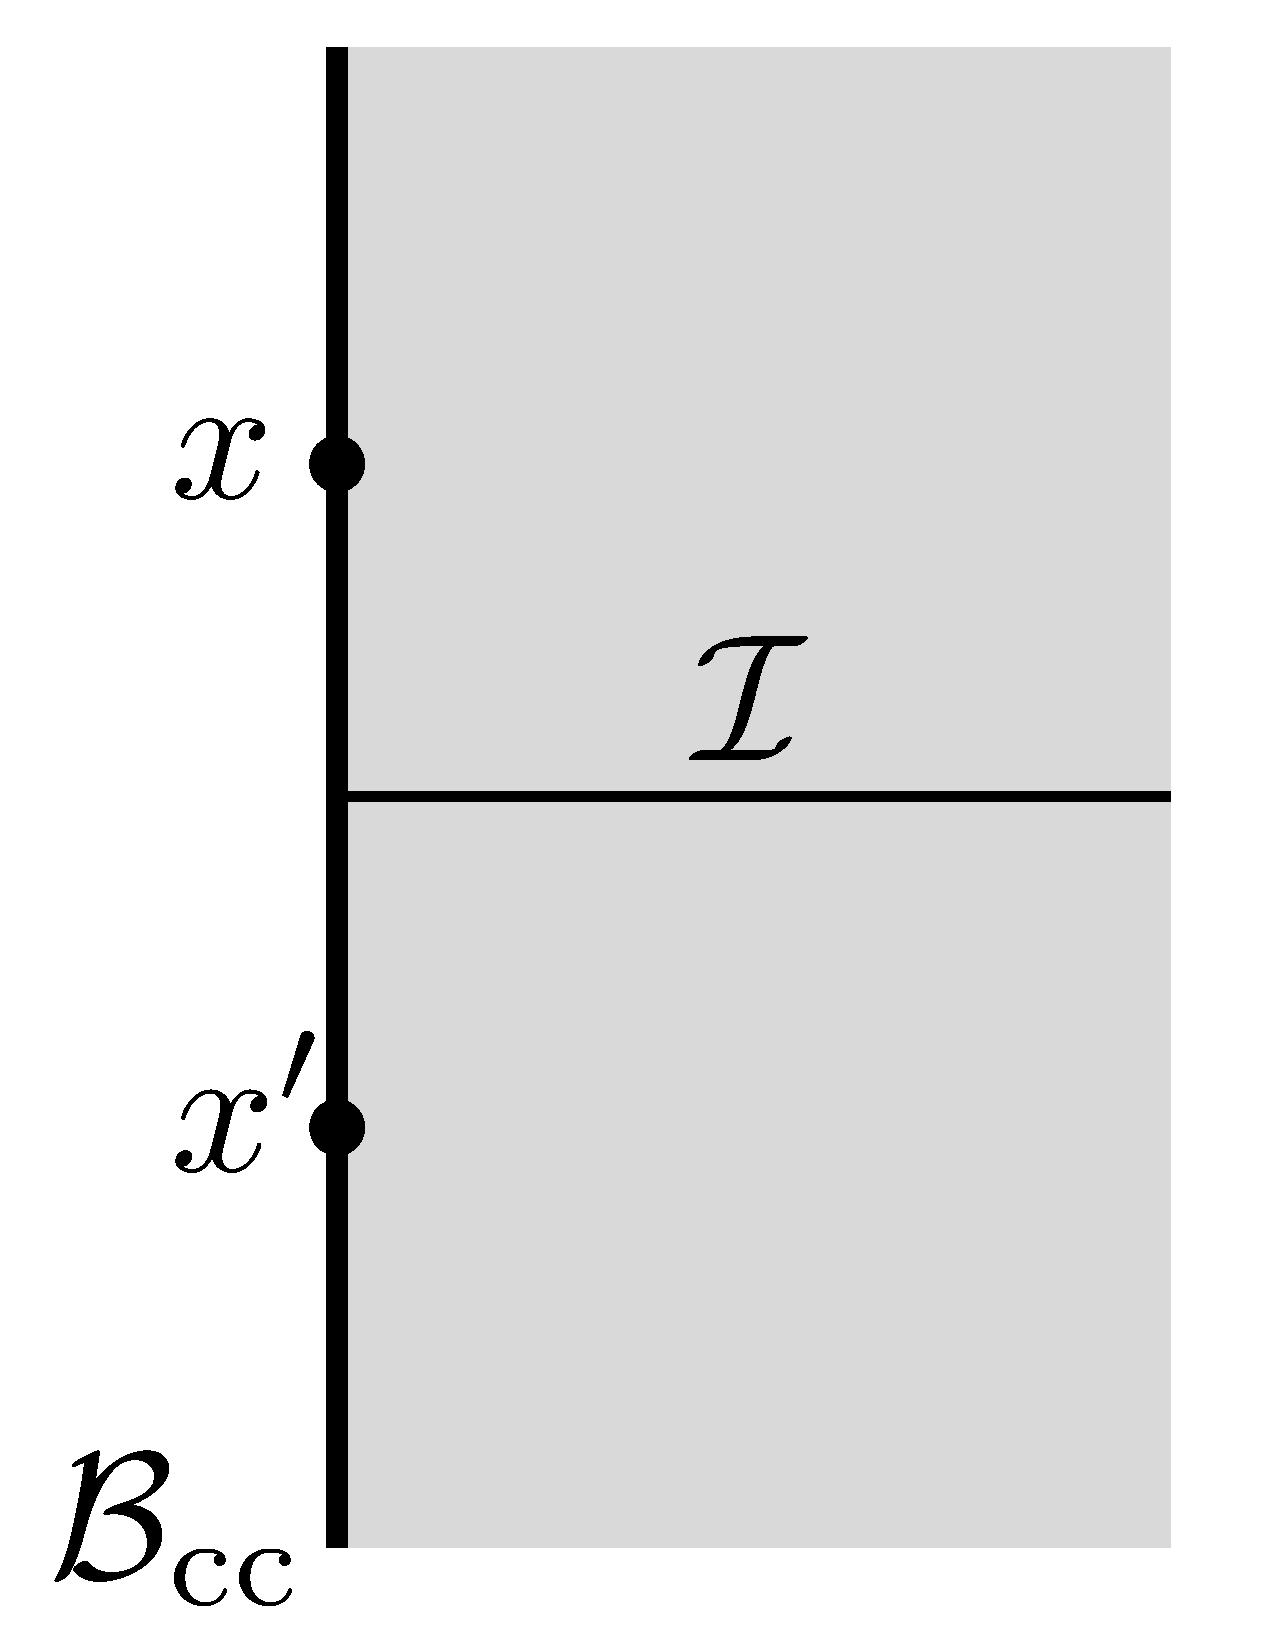
\includegraphics[width=0.28\textwidth]{figures/Pictorial.pdf}
 \caption{在界面 $\I$ 于膜 $\B_\cc$ 上的端点上方或下方插入的算符，分别给出边界算符代数 $\A$ 在 $\I$ 与 $\B_\cc$ 之间端点空间上的左作用或右作用。}\label{Pictorial}
\end{figure}

$\I$ 在 $\B_\cc$ 上结束的端点，在折叠图像中解释为 $\Hom(\h\B_\cc,\B_L)$ 的元素，其中 $\B_L$ 是支撑在 $L$ 上的拉格朗日膜，$\h\B_\cc$ 是 $Y\times Y'$ 两个因子上的余各向同性膜之积。$\Hom(\h\B_\cc,\h\B_\cc)$ 是两个 $\A=\Hom(\B_\cc,\B_\cc)$ 拷贝之积，每个因子对应一个。这两个拷贝作用在角空间 $\Hom(\h\B_\cc,\B_L)$ 上。因此展开后，两个 $\A$ 拷贝作用在 $\I$ 与 $\B_\cc$ 之间端点空间上。这一陈述有简单的图示解释（图 \ref{Pictorial}）：元素 $x\in\A$ 可以插在二维流形边界上给定端点的“下方”或“上方”。界面下方的插入对应于 $\A$ 在界面空间上的右作用，界面上方的插入对应于 $\A$ 的左作用。我们把带端点 $\alpha$ 的界面 $\I$ 记为 $\I(\alpha)$。对 $x\in\A$ 在 $\I(\alpha)$ 上的左作用或右作用，我们写 $\I(\alpha)\to x\I(\alpha)$ 或 $\I(\alpha)\to\I(\alpha)x'$。但由于 $x$ 只作用在 $\alpha$ 上，也可以更简单地写 $\alpha\to x\alpha$ 或 $\alpha\to\alpha x'$。

两个 $\A$ 拷贝在角空间 $\Hom(\h\B_\cc,\B_L)$ 上的作用，可更显式地看出如下。由附录 \ref{details}，$\Hom(\h\B_\cc,\B_L)$ 的首阶近似是
$H^0(L,\L\otimes K_L^{1/2})$，其中 $\L$ 是 $\B_L$ 的 $\CP$ 丛；为简单起见假设高阶上同调消失。由于 $L$ 嵌入 $Y\times Y'$，可以把 $H^0(L,\L\otimes K_L^{1/2})$ 的元素乘以 $Y$ 上的函数或 $Y'$ 上的函数。量子形变后，这给出两个 $\A$ 拷贝的作用。（“折叠”把代数映到反代数，其中算符按相反次序相乘；这就是为什么一个 $\A$ 拷贝以左作用、一个以右作用。）

作为一个重要的特殊情形，我们可以考虑生成代数 $\A$ 的自同构的界面 $\I$。这意味着存在角 $\alpha\in\Hom(\h\B_\cc,\B_L)$，使每个角都可唯一地写成 $x\alpha$（$x\in\A$），也可唯一地写成 $\alpha x'$（$x'\in\A$）。这一条件确定一个从 $\A$ 到自身的可逆映射 $\h\varphi$：对 $x\in\A$，$\h\varphi(x)$ 是使
$x\alpha=\alpha\h\varphi(x)$ 的 $\A$ 中元素。此外 $\h\varphi$ 可逆：对 $x\in\A$，$\h\varphi^{-1}(x)$ 是使 $\h\varphi^{-1}(x)\alpha=\alpha x$ 的 $\A$ 中元素。最后，$\h\varphi$ 是 $\A$ 的自同构，因为对 $x_1,x_2\in\A$，$x_1x_2\alpha=\alpha\h\varphi(x_1x_2)$，但另一方面 $x_1x_2\alpha=x_1\alpha\h\varphi(x_2)=\alpha\h\varphi(x_1)\h\varphi(x_2)$，故
$\h\varphi(x_1x_2)=\h\varphi(x_1)\h\varphi(x_2)$。

复常数在 $\A$ 的中心，也与界面交换，因此特别地，若 $\lambda$ 是非零复常数，则 $\lambda\alpha$ 生成与 $\alpha$ 相同的自同构。更一般地，设 $x_0$ 是 $\A$ 的任意可逆元。则对 $x\in\A$，有 $x(x_0\alpha)=x_0(x_0^{-1}xx_0)\alpha=x_0\alpha\h\varphi(x_0^{-1}xx_0)$，表明 $x_0\alpha$ 生成自同构 $x\to\h\varphi(x_0^{-1}xx_0)$。反之，若 $x_0\alpha$ 生成自同构，则角 $\alpha$ 等于某个 $x\in\A$ 的 $xx_0\alpha$，这意味着 $x_0$ 有逆 $x$。因此，若存在任何角 $\alpha$ 使给定界面生成自同构，则导致自同构的角恰为形如 $x_0\alpha$ 的角，其中 $x_0\in\A$ 可逆。

于是，在研究界面相伴的自同构时，若 $Y$ 使得常数是 $Y$ 上唯一的可逆（多项式）全纯函数，就会有一些简化。若假设 $b_1(Y)=0$，这其实是自动的；下文几处都会方便地作此假设。\footnote{设 $Y$ 上的全纯函数 $f$ 可逆，即处处不为零。则闭一形式 $\lambda=\d\log f$ 整体定义。若 $\lambda$ 恰当，$\lambda=\d u$（$u$ 为整体定义的全纯函数），则 $f=Ce^u$（$C$ 为非零常数），$f$ 在无穷远指数增长。若 $\lambda$ 不恰当，则 $\lambda$ 定义 $H^1(Y,\C)$ 的非零元素，$b_1(Y)>0$。}满足我们假设的典型例子是 $Y=\C^{2n}$，稍后我们会更仔细地研究。

现在设 $\varphi$ 是 $Y$ 的全纯辛同胚。它与复拉格朗日对应 $L\subset Y\times Y'$ 相伴，该对应参数化形如 $(y,\varphi(y))$ 的点。$L$ 有两个到 $Y$ 的映射，分别忘记 $Y\times Y'$ 的第一个或第二个因子，且每个映射都是同构。故作为复流形，$L$ 同构于 $Y$。特别地，$L$ 是复辛流形，故有典则 spin 结构。这给出折叠理论中膜 $\B_L$ 的典则选择，其 $\CP$ 丛 $\L$ 平凡；展开后它给出典则界面 $\I_L$。下文我们总作这一典则选择。又因 $b_1(Y)=0$ 且 $L$ 同构于 $Y$，$L$ 满足 $b_1(L)=0$。

反之，设 $\varphi,\varphi'$ 是 $Y$ 的两个全纯辛同胚，分别与复拉格朗日对应 $L,L'$ 及拓扑界面 $\I_\varphi,\I_{\varphi'}$ 相伴。由于 $L,L'$ 是复拉格朗日子流形，界面 $\I_\varphi$ 与 $\I_{\varphi'}$ 是 $(B,A,A)$ 型。如第 \ref{composing} 节所解释，这意味着（因 $b_1(L)=b_1(L')=0$）这些界面可以经典地合成，把它们视为 $B$-模型界面。该经典合成很容易描述。越过 $\I_\varphi$ 时，一般的 $\sigma$-模型场从 $X$ 跳到 $\varphi^*(X)$；越过 $\I_{\varphi'}$ 时，也有类似的从 $X$ 到 $\varphi'^*(X)$ 的跳变。由于我们取 $\CP$ 丛平凡，这就是全部。先越过 $\I_\varphi$ 再越过 $\I_{\varphi'}$，$X$ 先跳到 $\varphi^*(X)$，再跳到 $\varphi'^*(\varphi^*(X))$。最终结果是 $X$ 被映到 $(\varphi'\circ\varphi)^*(X)$。换言之，合成 $\I_\varphi\cdot\I_{\varphi'}$ 就是 $\I_{\varphi'\circ\varphi}$，其中 $\varphi'\circ\varphi$ 是两个辛同胚的合成。

虽然 $(B,A,A)$ 型界面可以在体内这样简单地合成，一般却没有同样简单的办法来合成它们与 $\B_\cc$ 的端点。一个例外是与 $\A$ 的自同构相关的情形。设 $\I_\varphi$ 与 $\I_{\varphi'}$ 分别带端点 $\alpha$ 与 $\alpha'$，生成 $\A$ 的自同构 $\h\varphi$ 与 $\h\varphi'$。这意味着对 $x\in\A$，有 $x\I_\varphi(\alpha)=\I_\varphi(\alpha)\h\varphi(x)$ 与 $x\I_{\varphi'}(\alpha')=\I_{\varphi'}(\alpha')\h\varphi'(x)$。合并这些关系，我们看到
\be\label{toolong}x\I_\varphi(\alpha)\I_{\varphi'}(\alpha')=\I_\varphi(\alpha)\h\varphi(x)\I_{\varphi'}(\alpha')=\I_\varphi(\alpha)\I_{\varphi'}(\alpha')\h\varphi'(\h\varphi(x)).\ee
换言之，令 $\varphi''=\varphi'\circ\varphi$，当我们合成 $\I_\varphi(\alpha)$ 与 $\I_{\varphi'}(\alpha')$ 时，端点的合成使得复合界面 $\I_{\varphi''}$ 带有一个端点 $\alpha''$，通过它生成自同构 $\h\varphi'\circ\h\varphi$。

为使这一点有意义，我们需要知道 $Y$ 有许多辛同胚，使得相应的界面配以合适端点后生成 $\A$ 的自同构。作为例子，我们考虑 $Y=\C^{2n}$ 及其标准复辛结构
$\Omega=\frac{1}{2\hbar}\sum_{i,j=1}^{2n}\omega_{ij}\d x^i\d x^j$。我们将用到一些伸缩论证，其成立理由如下。当我们用平坦超 Kähler 度量构造 $Y$ 的 $A$-模型时，所得的 $\sigma$-模型有保持该超 Kähler 度量的整体对称群 $\Sp_c(2n)$，以及旋转构成超 Kähler 结构一部分的三个复结构 $I,J,K$ 的 $R$-对称群 $\SU(2)_R$。特别地，$\SU(2)_R$ 有子群 $\UU(1)_R$，保持使 $\Omega$ 全纯的复结构 $I$ 不变。在 $\UU(1)_R$ 下，$x$ 的荷为 1，$\hbar$ 的荷为 2。这解释了下文将用到的一个伸缩对称。为得到另一个，先按通常方式把 $x$ 分成 $p$ 与 $q$，使 $\Omega=\frac1\hbar\sum_i\d p_i\d q^i$。于是（适当选取平坦超 Kähler 度量后）$\Sp_c(2n)$ 有子群 $\UU(1)'$，在它之下 $p$ 与 $q$ 的荷分别为 $1$ 与 $-1$（而 $\hbar$ 不变）。群 $\UU(1)_R\times\UU(1)'$ 有对角子群，在其下 $q$ 不变，而 $p$ 与 $\hbar$ 以相同方式伸缩；这解释了下文用到的另一个伸缩对称。

我们将解释如何从膜构造恢复 Kanel-Belov 与 Kontsevich \cite{BKK} 的结果：驯顺自同构群 $\TAut(\C^{2n})$ 作为 $\C^{2n}$ 上多项式函数的量子形变代数 $\A$（Weyl 代数）的自同构群作用。设 $\TAut_0(\C^{2n})$ 是 $\TAut(\C^{2n})$ 中这样的元素 $\varphi$ 构成的子集：相应的界面 $\I_\varphi$ 配以合适端点 $\alpha$ 后生成 $\A$ 的自同构 $\h\varphi$。上述论证表明，与 $\varphi$ 相伴的自同构 $\h\varphi$（存在时）唯一，且 $\TAut_0(\C^{2n})$ 至少是半群。此外，这个半群通过 $\A$ 的自同构作用。我们将证明第 \ref{oversym} 节描述的 $\TAut(\C^{2n})$ 的生成元属于 $\TAut_0(\C^{2n})$。因此 $\TAut(\C^{2n})$ 与 $\TAut_0(\C^{2n})$ 相同，并作为 $\A$ 的自同构群作用。

“$\TAut(\C^{2n})$ 的生成元属于 $\TAut_0(\C^{2n})$”这一陈述可由简单的伸缩论证推出。$\TAut(\C^{2n})$ 的一个生成元是线性辛同胚 $\varphi:\vec x\to A\vec x$，$A\in\Sp(2n,\C)$。在经典层面，$\h\B_\cc$ 与支撑在对应 $L$ 上的拉格朗日膜之间的角空间一般是 $H^i(L,\L\otimes K_L^{1/2})$，其中 $\L$ 是 $\CP$ 丛。在目前情形，$\L$ 与 $K_L^{1/2}$ 平凡，且 $L\cong\C^{2n}$，高阶上同调消失，故经典层面角空间约化为 $H^0(L,\O)$，即 $L$ 上全纯函数空间。经典上可取常数函数 $1\in H^0(L,\O)$，用它定义 $\B_L$ 与 $\h\B_\cc$ 之间的角，从而定义 $\I_\varphi$ 在 $\B_\cc$ 上的端点 $\alpha$。函数 1 在经典上不起作用；选取它意味着即使在 $\Sigma$ 边界上，界面的效果也只是导致从 $m$ 到 $\varphi(m)$ 的跳变。对辛同胚 $\varphi:\vec x\to A\vec x$，这意味着任何边界可观测量 $f(\vec x)$ 在经典层面跳到 $f(A\vec x)$：
\be\label{woro}f(\vec x)\I_\varphi(\alpha)=\I_\varphi(\alpha)f(A\vec x).\ee
这是经典公式。若 $f$ 非线性，则我们必须注意非交换代数 $\A$ 中因子的次序以及可能的量子修正，故一般不能指望量子形变理论中有如此简单的陈述。然而在目前情形有简单答案，因为要刻画界面对 $\A$ 的作用，只需说明 $\C^{2n}$ 上线性函数（它们生成代数 $\A$）会怎样。若 $x$ 是 $\C^{2n}$ 上任一线性函数，则公式
\be\label{oro}x\I_\varphi(\alpha)=\I_\varphi(\alpha)A(x)\ee
\emph{不}受任何量子修正。这可由前面解释的 $\UU(1)_R$ 伸缩推出，其中 $x$ 按次数 1 伸缩，$\hbar$ 按次数 2 伸缩。由于 $\A$ 的所有元素次数非负，这个伸缩对称不给式 \eqref{oro} 留下任何修正的余地。

按通常方式把 $x$ 分成 $p$ 与 $q$ 后，辛形式变为 $\Omega=\sum_i\d p_i\d q^i/\hbar$，$\TAut$ 的其他生成元取形式
\begin{align}\label{koro}\varphi^*(p_i)&=p_i+\partial f/\partial q^i,\cr
\varphi^*(q^i)&=q^i.\end{align}
设 $L_f$ 是与此辛同胚相伴的对应，$\I_f$ 是相应界面。配以与常数函数 $1\in H^0(L,\O)$ 相伴的端点 $\alpha$ 后，界面 $\I_f$ 实现式 \eqref{koro} 所示的自同构，其意义是
$q^i\I_f(\alpha)=\I_f(\alpha)q^i$，且 $p_i\I_f(\alpha)=\I_f(\alpha)(p_i+\partial f/\partial q^i)$，至少在 $\hbar\to0$ 的极限下如此。我们前面解释过，在 $f=0$ 时有伸缩对称，其中 $p$ 与 $\hbar$ 次数为 1，而 $q$ 次数为 0。我们可以说 $f$ 次数为 1，把它延拓到 $f\ne0$ 的情形。这个伸缩对称不给公式留下任何修正余地，因为它在 $f=0$ 时成立（此时界面平凡，$\varphi^*(p_i)=p_i$，没有 $\hbar$ 阶修正）。故这些额外生成元也含于 $\TAut_0(\C^{2n})$ 中。

理想地，人们想类似地证明：不仅 $\TAut(\C^{2n})$，而且可能更大的群 $\Aut(\C^{2n})$ 也作为 $\A$ 的自同构群作用，正如 \cite{BEY} 所证明的那样。主要困难如下。设 $\varphi$ 是 $\C^{2n}$ 的一个假想多项式辛同胚，不包含在 $\TAut(\C^{2n})$ 中；设 $L$ 与 $\I_\varphi$ 是相应的对应与界面。人们想断言 $\I_\varphi$ 与 $\B_\cc$ 之间存在与函数 $1\in H^0(L,\O)$ 相伴的典则端点，但这需要对 $L$ 有所了解，如附录 \ref{corrections} 所解释。然后希望证明配以典则端点的 $\I_\varphi$ 实现 $\A$ 的自同构；再借助与 $B$-模型的关系证明这些自同构正确合成，就完成了 $\TAut(\C^{2n})$ 是 $\A$ 的自同构群的论证。对子群 $\TAut(\C^{2n})$，我们能够跳过其中大部分步骤，因为可以直接看出 $\TAut(\C^{2n})$ 的生成元确实实现自同构。如附录 \ref{corrections} 所解释，由于生成元结构简单，可以直接证明典则端点对它们存在；但对假想的非驯顺 $\varphi$，则需要更精细的论证。

至此我们只考虑了形变量子化。在第 \ref{qtz} 节中，我们将解释类似的量子化讨论需要哪些新要素。但在 $\R^{2n}$ 这个重要的特殊情形中，我们可以立即以一种\emph{权宜}的方式做到。为得到量子化的对称，我们应把 $\TAut(\C^{2n})$ 限制到其子群，该子群由限制到 $\R^{2n}$ 上为实辛同胚的元素组成。我们称此子群为 $\TAut(\R^{2n})$。$\TAut(\R^{2n})$ 由线性辛同胚 $\vec x\to A\vec x$（现在 $A\in\Sp(2n,\R)$）连同变换 \eqref{koro}（现在 $f$ 限制为实）生成。

根据已学到的内容，不难证明 $\TAut(\R^{2n})$，更确切地说是它由 $\UU(1)$ 作的中心扩张，作为酉变换群作用在量子化 $\R^{2n}$ 所得的 Hilbert 空间 $\H$ 上。首先检验 $\TAut(\R^{2n})$ 的生成元可实现为 $\H$ 上的酉变换，且通过共轭生成 $\A$ 的预期自同构。对线性辛同胚 $\vec x\to A\vec x$，这正是熟知的事实：群 $\Sp(2n,\R)$（更确切地说是它的二重覆盖）酉作用于 $\H$。至于式 \eqref{koro} 的变换 $p_i\to p_i+\partial_i f(q)$，若把 $\H$ 实现为 $q$ 的函数 $\psi(q^1,q^2,\cdots,q^n)$ 的空间，则该变换由乘以 $\exp(\i f(q)/\hbar)$ 的酉算符实现。

给定任意 $\varphi\in\TAut(\R^{2n})$，可把它写成该群生成元的字。然后把生成元对应的酉变换相乘，得到与 $\varphi$ 相伴的酉变换 $U_\varphi$。把 $\varphi$ 写成生成元的字的另一种方式，可能给 $\varphi$ 相伴另一个酉变换 $\t U_\varphi$。然而我们已知 $\TAut(\R^{2n})$ 作为 $\A$ 的对称群作用，故 $U_\varphi$ 与 $\t U_\varphi$ 都必须通过共轭生成与 $\varphi$ 相伴的自同构。由于 $\H$ 上与 $\A$ 交换的算符只有复标量，这意味着必须有 $\t U_\varphi=e^{\i\alpha}U_\varphi$，其中 $e^{\i\alpha}\in\UU(1)$。因此对应 $\varphi\to U_\varphi$ 表示中心扩张
\be\label{centex}1\to\UU(1)\to\TAut^*(\R^{2n})\to\TAut(\R^{2n})\to1\ee
在 $\H$ 上的作用。这个中心扩张非平凡，且不能约化为由 $\R^{2n}$ 的真子群作的中心扩张。确实，$\TAut(\R^{2n})$ 包含平移群 $\vec x\to\vec x+\vec b$，而仅仅要把这个群实现为量子对称群，就需要由 $\UU(1)$ 作的中心扩张。若限制到 $\TAut(\R^{2n})$ 中保持 $\R^{2n}$ 中指定点不变的子群，中心扩张可能约化为有限子群（可能是 $\Z_2$）的扩张。

\subsection{应用于量子化}\label{qtz}

接下来我们想得到与第 \ref{symmeq} 节形变量子化结果类似的量子化结果。为此，我们特殊化到这样的情形：$Y$ 的复辛同胚 $\varphi$ 是 $M$ 的实辛同胚 $\varphi_r$ 的解析延拓。我们假设 $\varphi_r$ 提升为预量子线丛 $\frL\to M$ 的对称；换言之，假设 $\varphi_r^*(\frL)$ 与 $\frL$ 作为带联络的酉线丛同构。记 $L_r$ 为 $M\times M'$ 中与 $\varphi_r$ 相伴的拉格朗日对应，$L$ 为其在 $Y\times Y'$ 中的复化。设 $\I_\varphi$ 是 $Y$ 的 $A$-模型中相应的拓扑界面。上一节讨论了 $\I_\varphi$ 在 $\B_\cc$ 上的端点 $\alpha$ 的性质，使 $\I_\varphi$ 实现代数 $\A$ 的自同构。为了使 $\I_\varphi$ 不仅作用于 $\A$，而且作用于量子 Hilbert 空间，即作用于 $A$-模 $\H=\Hom(\B,\B_\cc)$，我们还需要一个端点 $\beta$，使 $\I_\varphi$ 在支撑于 $M$ 的拉格朗日膜 $\B$ 上结束。

在折叠图像中，$\B$ 来自支撑在 $M\times M'\subset Y\times Y'$ 上的拉格朗日膜 $\h\B$，其 Chan--Paton 丛为 $\frL^{-1}\boxtimes\frL$（第二个因子是第一个的逆，因为折叠把 $\CP$ 丛换成其对偶）。界面 $\I_\varphi$ 在折叠图像中来自支撑在 $L$ 上的拉格朗日膜 $\B_L$，其 $\CP$ 丛平凡。角空间 $\Hom(\B_L,\h\B)$ 的首阶近似，就是交 $L\cap(M\times M')$ 上取值于 $\CP$ 丛张量积的 de Rham 上同调。由于 $\B_L$ 的 $\CP$ 丛平凡，相关的 $\CP$ 丛之积就是 $\frL^{-1}\boxtimes\frL$。

交 $L\cap(M\times M')$ 就是实拉格朗日对应 $L_r$。由于 $L_r$ 参数化 $M\times M'$ 中形如 $(m,\varphi_r(m))$ 的对，它在拓扑上是 $M$ 的一个拷贝。为简单起见，假设 $b_1(M)=0$（我们继续假设 $b_1(Y)=0$）。这意味着 $b_1(L_r)=0$，且 $A$-模型空间 $\Hom(\B_L,\h\B)$ 就是 $L_r$ 上取值于 $\frL^{-1}\boxtimes\frL$ 的 de Rham 上同调。作为 $M\times M'$ 上的线丛，$\frL^{-1}\boxtimes\frL$ 当然不平凡；但 $\varphi_r^*(\frL)$ 与 $\frL$ 同构的假设意味着，限制到 $L_r$ 上时 $\frL^{-1}\boxtimes\frL$ 平凡。$\varphi_r^*(\frL)$ 与 $\frL$ 之间的同构在乘以模 1 复数的意义下唯一。每个同构 $\beta:\frL\to\varphi^*(\frL)$ 的选择，都确定 $H^0_{\mathrm{dR}}(L_r,\frL^{-1}\boxtimes\frL)$ 的一个元素 $\beta$。这些就是 $\I_\varphi$ 与 $\B$ 之间的典则端点。

这类角在 $\sigma$-模型映射 $\Phi:\Sigma\to Y$ 的语言中有简单含义。$\Phi$ 把二维流形 $\Sigma$ 映到 $Y$，同时把由 $\B$ 标记的 $\partial\Sigma$ 的一个分支映到 $M$。在界面 $\I_\varphi$ 与 $\partial\Sigma$ 相遇的端点 $\sigma$ 处，映射 $\Phi:\partial\Sigma\to M$ 不连续，从 $m$ 跳到 $\varphi(m)$。重要的是，若用类 $\beta\in H^0_{\mathrm{dR}}(L_r,\frL^{-1}\boxtimes\frL)$ 定义端点，则对 $\Phi(\sigma)$ 的行为没有进一步限制。反之，若用例如 $H^k_{\mathrm{dR}}(L_r,\frL^{-1}\boxtimes\frL)$ 中 Poincaré 对偶于余维 $k$ 子流形 $V\subset L_r$ 的元素，则我们必须施加约束 $\Phi(\sigma)\in V$。

“无约束”条件在合成界面时能很好地自我复制。设 $\varphi_r,\varphi_r'$ 是 $M$ 的两个实辛同胚，都提升为 $\frL$ 的对称；定义 $\varphi_r''=\varphi_r'\circ\varphi_r$。在体内，与 $B$-模型的关系表明相应界面按自然方式合成：$\I_{\varphi'}\cdot\I_\varphi=\I_{\varphi''}$。我们希望给它们配上与 $\B$ 的端点，使这一简单合成律在界面于 $\B_\cc$ 上结束时仍成立。为此，我们使用与同构 $\beta:\frL\to\varphi_r^*(\frL)$、$\beta':\frL\to\varphi_r'{}^*(\frL)$ 相伴的简单端点。如上段所述，当界面 $\I_\varphi$ 或 $\I_{\varphi'}$ 在 $\partial\Sigma$ 上结束时，这样的端点不施加约束。“无约束”与“无约束”的合成仍是“无约束”。若用 $\beta''=\beta'\circ\beta$ 定义 $\beta'':\frL\to\varphi_r''{}^*(\frL)$，则包括其在 $\partial\Sigma$ 上的端点在内，界面的合成就简单地是 $\I_{\varphi'}(\beta')\cdot\I_\varphi(\beta)=\I_{\varphi''}(\beta'')$。

关于这个答案，有几点值得强调。第一，对这些界面在拉格朗日膜 $\B$ 上的端点，这个答案比我们在其于 $\B_\cc$ 上的端点所得到的答案直接得多。第二，为得到这个答案，我们必须考虑由辛同胚 $\varphi_r:M\to M$ 连同同构 $\beta:\frL\to\varphi^*(\frL)$ 组成的对。这样的对正是经典力学对称群 $\G$ 的元素，如第 \ref{problem} 节所定义。

现在设 $\T$ 是 $Y$ 的复辛同胚的集合，这些辛同胚在配上与 $\B_\cc$ 的合适角后生成 $\A$ 的自同构。于是对任何 $\varphi\in\T$，界面 $\I_\varphi$ 有端点 $\alpha$，使 $\I_\varphi(\alpha)$ 生成自同构。我们在第 \ref{symmeq} 节得知 $\T$ 是群，而且作为 $\A$ 的自同构群作用。设 $\T_r$ 是 $\T$ 中这样的辛同胚构成的子群：它们把 $M$ 映到自身，且限制到 $M$ 上时提升为 $\frL$ 的对称。由于与辛同胚相伴的 $\frL$ 对称只在整体相位意义下唯一，$\T_r$ 出现在中心扩张
\be\label{zirko}1\to\UU(1)\to\T_r^*\to\T_r\to1\ee
中。每个 $\varphi\in\T_r$ 都是某个 $\varphi_r:M\to M$ 的解析延拓，使得存在同构 $\beta:\frL\to\varphi_r^*(\frL)$。这个同构可用于定义 $\I_\varphi$ 在 $\B$ 上的端点，我们也称之为 $\beta$。给每个 $\varphi\in\T_r$ 的 $\I_\varphi$ 配上这样的端点 $\alpha,\beta$，我们定义作用在 $\H=\Hom(\B,\B_\cc)$ 上的量子算符 $\O_{\varphi,\alpha,\beta}$。鉴于关于体算符与端点的讨论，这些算符 $\O_{\varphi,\alpha,\beta}$ 能正确合成，给出群 $\h\T_r$ 在 $\H$ 上的作用。在第 \ref{symmeq} 节末尾，我们对 $M=\R^{2n}$ 演示了这一点，其方式依赖于该情形中代数 $\A$ 相当大这一事实。然而，即使 $\A$ 不那么大，结果仍成立。

\subsection{酉性}\label{hermcon}

最后，我们解释构造出的辛同胚算符的酉性。我们的讨论基于第 \ref{hermitian} 节的框架。要定义伴随，需要算子空间上的 Hermite 内积。这里我们可以分两步。首先，对偶或转置算符可由把双向图旋转 $\pi$（或等价地，把图从下往上读）得到。与辛同胚 $\varphi$ 相伴的界面的转置，来自 $\varphi^{-1}$。然后，若 $A$-模型有反辛对合 $\tau$，且膜 $\B_1,\B_2$ 为 $\tau$-不变，则 $\Hom(\B_1,\B_2)$ 有 Hermite 度量，伴随由
\be\label{wedj}\O^\dagger=\Theta_\tau\O^*\Theta_\tau\ee
给出，其中 $\O^*$ 是转置算子。

在我们的量子化情形，$\B_1=\B$（支撑在 $M$ 上的拉格朗日膜），$\B_2=\B_\cc$。若 $\varphi$ 是 $M$ 的辛同胚 $\varphi_r$ 的解析延拓，则 $\varphi$ 为 $\tau$-不变，即 $\tau\varphi\tau=\varphi$。这蕴含 $\tau\varphi^{-1}\tau=\varphi^{-1}$。因此 $\O^\dagger$ 来自界面 $\I_{\varphi^{-1}}$。于是 $\O^\dagger\O$ 来自 $\I_{\varphi^{-1}}\cdot\I_\varphi=\I_{\text{平凡}}$。平凡界面配上平凡端点，给出恒等算符乘以某个模 1 的复数。最后，算符 $\O^\dagger\O$ 非负，故该复数必为 1：
\be\label{kunu}\O^\dagger\O=1.\ee
因此构造出的辛同胚算符都是酉的。

\section{量子化复流形}\label{qcomp}

本节我们转向一个多少有些不同的方向。设 $Y$ 是复辛流形，带全纯辛形式 $\Omega$。通过忘记其复结构，可把 $Y$ 视为实辛流形。我们想用量子化来解释复流形 $Y$ 的量子化，即把 $Y$ 的量子化定义为把 $Y$ 视为实流形时的膜量子化。

沿用第 \ref{amo} 节的记号，$Y$ 作为实辛流形的典范复化是 $\h Y=Y_1\times Y_2$，其中 $Y_1$ 与 $Y_2$ 都同构于 $Y$，但复结构相反。因此 $\h Y$ 作为实流形带有两个复结构 $I_1=I\oplus I$ 与 $I_2=-I\oplus(-I)$。交换两个因子的对合
\be\label{qcomplextwo}\tau:(y_1,y_2)\mapsto(\bar y_2,\bar y_1)\ee
是反全纯的，其不动点集是对角 $\Delta\cong Y$。这是 $\h Y$ 中实维数为 $\dim_\C Y$ 的实子流形。$\tau$ 与 $\h Y$ 上的复辛形式
\be\label{qcomplexone}\h\Omega=\frac12\Omega\boxplus\frac12\bar\Omega\ee
相容，其中 $\Omega$ 是 $Y_1$ 上的全纯辛形式，$\bar\Omega$ 是 $Y_2$ 上的全纯辛形式（在 $Y_2$ 的复结构下）。限制到对角 $\Delta$ 上，$\h\Omega$ 等于 $\Re\Omega$。因此我们取 $\h Y$ 的实辛形式为 $\Im\h\Omega$，使 $\Delta$ 为拉格朗日。相应地，B-场为 $\Re\h\Omega=\frac12\Re\Omega\boxplus\frac12\Re\Omega$，限制到 $Y$ 上就是 $\Re\Omega$。

现在我们来描述 $\h Y$ 上的典范余各向同性膜 $\h\B_\cc$。在 $Y_1$ 上，$\sF+\sB=\frac12\Re\Omega=\frac12\omega_J$，复合结构 $\omega^{-1}(\sF+\sB)$ 等于 $(\frac12\omega_K)^{-1}(\frac12\omega_J)=I$，其中 $I$ 是 $Y_1$ 的复结构。在 $Y_2$ 上，复结构是 $-I$，而 $\omega^{-1}(\sF+\sB)=(\frac12\omega_K)^{-1}(\frac12\omega_J)=I$，故相对于 $Y_2$ 的复结构，它等于 $-I$。因此在 $Y_1$ 与 $Y_2$ 上，$\sF+\sB$ 都给出可积复结构，$\B_{\cc,1}$ 与 $\B_{\cc,2}$ 都是 $\h Y$ 上的典范余各向同性膜，其 $\CP$ 丛平凡。乘积 $\h\B_\cc=\B_{\cc,1}\times\B_{\cc,2}$ 是 $\h Y$ 上的典范余各向同性膜。

$\h Y$ 上的拉格朗日膜 $\h\B$ 支撑在对角 $\Delta\cong Y$ 上。为满足 $\sF+\sB=0$，需取 $\sF=-\Re\Omega$。由于 $\frL$ 是 $Y$ 上曲率为 $\Re\Omega$ 的预量子线丛，$\h\B$ 的 $\CP$ 丛可取为 $\frL^{-1}$。与通常一样，反常条件因复辛流形有典则 spin 结构而自动满足。于是所预想的量子 Hilbert 空间是
$\H=\Hom(\h\B,\h\B_\cc)$。

与形变量子化的关系是清楚的。我们有
\[\Hom(\h\B_\cc,\h\B_\cc)=\Hom(\B_{\cc,1},\B_{\cc,1})\times\Hom(\B_{\cc,2},\B_{\cc,2}).\]由第 \ref{abranes} 节，$\Hom(\B_{\cc,1},\B_{\cc,1})=\A$ 是 $Y$ 上全纯函数的形变量子化，而 $\Hom(\B_{\cc,2},\B_{\cc,2})=\bar\A$ 是反全纯函数的形变量子化。因此 $\Hom(\h\B_\cc,\h\B_\cc)=\A\times\bar\A$，正如把 $Y$ 视为实辛流形时 $\Hom$ 代数所应为。

我们可以像 §\ref{abranes} 那样展开这个构造。假设 $\frL=\L^2$ 是某个线丛的平方，使 $c_1(\frL)$ 为偶。作一个 B-场变换，可令 $\sB=0$，于是两个 $\B_\cc$ 的 $\CP$ 丛都是 $\L$（其曲率为 $\frac12\omega_J$），而 $\h\B$ 的 $\CP$ 丛平凡。$(\h\B,\h\B_\cc)$ 弦的世界面是条带 $\R\times[0,\pi]$：在 $\sigma=0$ 处边界条件由 $\h\B_\cc$ 给出，它是乘积膜，与展开无关；在 $\sigma=\pi$ 处边界条件由 $\h\B$ 给出，它不是乘积膜，把 $Y$ 的两个拷贝粘在一起。

因为 $\h\B$ 支撑在对角上，展开后得到 $[0,2\pi]$ 上单个 $Y$ 的 $\sigma$-模型，其边界条件在 $\sigma=0$ 与 $\sigma=2\pi$ 处由两个（不同的）膜给出。具体地，把 $\sigma>\pi$ 的部分翻转，会改变其定向，等价于改变辛形式的符号；这使两半上的辛形式都变为 $\omega_K$。边界定向的反转把 $\CP$ 丛取逆，故在 $\sigma=2\pi$ 处膜的 $\CP$ 曲率为 $-\frac12\omega_J$，即它是共轭膜 $\bar\B_\cc$。于是展开后的 $\Hom(\h\B,\h\B_\cc)$ 被重新解释为 $\Hom(\bar\B_\cc,\B_\cc)$。

我们本可以先取 $\sB\ne0$ 再展开，但那样 B-场在条带中央会不连续，该不连续处成为一个拓扑线算符。先令 $\sB=0$ 的代价是假设 $\frL$ 有平方根。在与几何 Langlands 相关的情形（\cite{GaW}），$\omega_J$ 的上同调平凡，而 $\frL$ 平凡，故无 B-场的版本更为方便。

\begin{yizhu}[本节与几何 Langlands 的关系]
把复辛流形 $Y$ 当作“实辛流形 $Y$”来量子化，听起来玄，其实是几何 Langlands 里的标准图像：Hitchin 模空间既是复辛流形，又是某个实辛流形的复化；其 $A$-模型给出 $D$-模侧，$B$-模型（全纯函数的形变量子化）给出 Higgs 丛侧。原文 §\ref{flatg} 中“$H^0(M,K_M^{1/2}\otimes\frL)$ 与复结构 $t$ 无关”的陈述，正是这一图像最可检验的推论之一；沿 Teichmüller 空间移动 $t$ 给出的平坦联络（ADW、Hitchin、Faltings），则是它的几何实现。[来源：A 级]
\end{yizhu}

\medskip
\noindent{\bfseries 致谢}\quad
我们感谢 M. Abouzeid、R. Bezrukavnikov、K. Costello、E. Frenkel、P. Etingof、V. Ginzburg、D. Kazhdan、S. Li 与 R. Mazzeo 的讨论。

Perimeter Institute 的研究由加拿大政府通过 Industry Canada 以及安大略省研究与创新部资助。E. Witten 的研究部分由 NSF 基金 PHY-1911298 资助。

\appendix

\section{反常}\label{anomaly}

为说明从经典力学过渡到量子力学时的反常，我们考虑 $\R^2$，用泊松括号 $\{x_1,x_2\}=1$ 的实变量 $x_1,x_2$ 参数化。量子化后，$x_1$ 与 $x_2$ 成为满足 $[\h x_1,\h x_2]=-\i\hbar$ 的算符 $\h x_1,\h x_2$。在分析量子化问题时，我们假设 $x_i$ 的任一 $k$ 次多项式（$k\ge1$）的量子化应是 $\h x_i$ 的 $k$ 次多项式，且首项相同。问题在于：能否选择量子算符中因子的次序以及可能的低阶项，使换位子与泊松括号精确相符。

单项式 $x_{i_1}x_{i_2}\cdots x_{i_k}$ 的 Weyl 排序 $\left\langle\h x_{i_1}\h x_{i_2}\cdots\h x_{i_k}\right\rangle$ 定义为对因子 $k!$ 种可能次序的平均：
\be\label{weyl}\left\langle\h x_{i_1}\h x_{i_2}\cdots\h x_{i_k}\right\rangle=\frac{1}{k!}\left(\h x_{i_1}\h x_{i_2}\cdots\h x_{i_k}+\h x_{i_2}\h x_{i_1}\cdots\h x_{i_k}+\cdots\right).\ee
我们一开始并不假设 Weyl 排序是给因子排序的最佳方式。我们将看到，无论怎样排列因子、添加怎样的低阶项，都无法避免 $x_1,x_2$ 的多项式量子化中的反常。在下面将解释的意义上，Weyl 排序最接近避免反常。

对次数 $\le2$ 的多项式没有反常。次数 $\le2$ 的 Weyl 排序多项式的换位子，按预期方式与相应经典多项式的泊松括号相符。Weyl 排序是具有这一性质的唯一做法：给次数 $\le2$ 的 Weyl 排序多项式添加低阶项会改变其换位子。我们假设这一点已知（或读者会自行验证），并说明若考虑次数大于 $2$ 的多项式，就会出现反常。

$x_1$ 与 $x_2$ 的齐二次多项式，即 $x_1^2$、$x_2^2$ 与 $x_1x_2$，通过泊松括号生成 Lie 代数 $\SL(2,\R)$。$x_1,x_2$ 的 $k$ 次齐次多项式张成 $k+1$ 维向量空间，并按 $\SL(2,\R)$ 的 $k+1$ 维不可约表示变换。由于二次多项式无反常，$\h x_1,\h x_2$ 的 Weyl 排序二次多项式，即 $\h x_1^2$、$\h x_2^2$ 与 $\frac12(\h x_1\h x_2+\h x_2\h x_1)$，也通过换位子生成 $\SL(2,\R)$ 的 Lie 代数。$\h x_1,\h x_2$ 的 $k$ 次 Weyl 排序齐次多项式，像其经典对应物一样，按 $\SL(2,\R)$ 的 $k+1$ 维不可约表示变换。任何其他次序选择（等价地，给 $k$ 次 Weyl 排序多项式添加任何低阶项）都会破坏这一事实，因为次数小于 $k$ 的多项式按 $\SL(2,\R)$ 的较小表示变换。因此，当且仅当使用 Weyl 排序时，齐二次多项式与任意 $k$ 次齐次多项式的换位子才无反常。

然而，两个次数大于 $2$ 的 Weyl 排序多项式的换位子会出现反常。为说明这一点，只需在一个特殊情形中展示反常。令 $z=(x_1-\i x_2)/\sqrt2$、$\bar z=(x_1+\i x_2)/\sqrt2$，则 $\{z,\bar z\}=\i$ 且 $[\h z,\h{\bar z}]=\hbar$。我们有 $\{z^3,\bar z^3\}=9\i z^2\bar z^2$，故若无反常，就应要求
$[z^3,\bar z^3]=9\hbar\left\langle\h z,\h z,\h{\bar z},\h{\bar z}\right\rangle$。但简单计算表明，实际有
\be\label{tofo}[\h z^3,\h{\bar z}^3]=9\hbar\left\langle\h z,\h z,\h{\bar z},\h{\bar z}\right\rangle+\frac32\hbar^3,\ee
\begin{kanwu}[一处指数笔误]
原文式 \eqref{tofo} 左端写作 $[\h z^3,\h{\bar z}^2]$，与上下文（$\bar z^3$）不符；此处按文意改为 $\bar z^3$。
\end{kanwu}

这就展示了反常。

在这个特殊例子中，换位子里的反常项是 $c$-数。对更高次的多项式，比如 $z^3$ 与 $\bar z^4$，情况并非如此。这一断言无需进一步计算，由 Jacobi 恒等式
$[\h z,[\h z^3,\h{\bar z}^4]]+[\h{\bar z}^4,[\h z,\h z^3]]+[\h z^3,[\h{\bar z}^4,\h z]]=0$
即可推出。

\section{关于 $\Hom(\B_\cc,\B_\cc)$ 与 $\Hom(\B,\B_\cc)$ 的细节}\label{details}

\subsection{最低阶计算}

本附录的目的是概述 $\Hom(\B_\cc,\B_\cc)$ 与 $\Hom(\B,\B_\cc)$ 的计算，其中 $\B$ 是拉格朗日 $A$-膜。计算在 $\sigma$-模型微扰论的最低阶进行。可能的修正将在附录 \ref{corrections} 中讨论。

为具体定义复辛流形 $Y$ 的 $A$-模型（辛结构为 $\omega=\omega_K$），需要 $Y$ 上一个近复结构，使 $\omega_K$ 关于它为 $(1,1)$ 型且正。若 $Y$ 容许一个延拓其辛结构的超 Kähler 结构（意义见第 \ref{amo} 节），我们可以使用作为辛结构一部分的复结构 $K$。即使 $Y$ 不容许这样的超 Kähler 结构，也总能在 $Y$ 上取一个近超 Kähler 结构，即选取近复结构 $J$ 与 $K$，使它们（连同 $Y$ 的复辛结构）满足第 \ref{amo} 节讨论的代数关系。这之所以可能，理由如下。设 $Y$ 的实维数为 $4k$。$Y$ 的复辛结构把其切丛的结构群从 $\GL(4k,\R)$ 约化为 $\Sp(2k,\C)$。$\Sp(2k,\C)$ 的最大紧子群是紧形式 $\Sp_c(2k)$。商 $\Sp(2k,\C)/\Sp_c(2k)$ 可缩，故一旦切丛的结构群约化为 $\Sp(2k,\C)$，进一步约化到 $\Sp_c(2k)$ 就没有障碍。这正是定义 $J$、$K$ 以及 $Y$ 上满足通常代数关系的度量 $g$ 所需的结构。此外，任何两个这样的约化都同伦，因而给出等价的 $A$-模型。在下面的分析中，我们假设 $K$ 是某个近超 Kähler 结构的一部分。

首先考虑 $\Hom(\B_\cc,\B_\cc)$，沿用 \cite{GW} 第 2.2 节。考虑条带 $\Sigma=\R\times[0,\pi]$ 上的 $(\B_\cc,\B_\cc)$ 弦，第二个因子由 $\sigma$ 参数化。一般地，$\sigma$-模型的自由度是描述映射 $\Phi:\Sigma\to Y$ 的玻色场 $X$，以及取值于 $\Phi^*(TY)\otimes\SS_\pm$ 的费米场 $\psi_\pm$（$\SS_+$ 与 $\SS_-$ 是 $\Sigma$ 的正、负手征旋量丛）。$A$-模型微分 $Q$ 生成的 $X$ 的一般变换为
\be\label{windo}\delta X=(1-\i K)\psi_++(1+\i K)\psi_-.\ee
这意味着 $\delta X$ 有正比于 $\psi_+$ 的 $(1,0)$ 部分，以及正比于 $\psi_-$ 的 $(0,1)$ 部分。由于在 $\Sigma$ 内部，$\psi_+$ 与 $\psi_-$ 是 $\Phi^*(TY)\otimes\SS_\pm$ 的截面且不受特殊约束，为使 $\Sigma$ 内部的算符 $F(X,\bar X)$ 为 $Q$-不变，函数 $F$ 必须是常数。但我们关心的是插在边界上的局部算符，这里情况不同。一般地 \cite{ACNY}，在 CP 丛曲率为 $\sF$ 的秩 1 膜上、且存在二形式场 $\sB$ 时，世界面费米子满足边界条件
\be\label{wiffo}\psi_+=(g-(\sF+\sB))^{-1}(g+\sF+\sB)\psi_-.\ee
对 $\B_\cc$，$\sF+\sB=\omega_J$，边界条件化为
\be\label{nelm}\psi_+=J\psi_-,\ee
于是沿 $\Sigma$ 的边界，$X$ 的变分化为 $\delta X=(1+\i I)(1+J)\psi_-$。这意味着相对于复结构 $I$，沿 $\Sigma$ 的边界 $\delta X$ 只有 $(0,1)$ 部分：
\begin{align}\label{btrans}\delta^{1,0}X&=0,\cr
\delta^{0,1}X&=\rho,\end{align}
其中 $\rho=(1+\i I)(1+J)\psi_-$。由于 $Q^2=0$，式 \eqref{btrans} 表明沿 $\partial\Sigma$ 有
\be\label{bcorr}\delta\rho=0.\ee
在 $\rho$ 中次数为 $q$ 的边界算符 $F(X,\bar X,\rho)$ 对应于 $Y$ 上的 $(0,q)$-形式，而式 \eqref{btrans}、\eqref{bcorr} 表明 $Q$ 作用在这些算符上就如复结构 $I$ 中通常的 $\bar\partial$ 算符。因此在这个近似下，物理态空间是上同调 $\oplus_{q=0}^{\dim_\C Y}H^q(Y,\O)$。

现在考虑 $\Hom(\B,\B_\cc)$，其中 $\B$ 是秩 1 拉格朗日 $A$-膜，支撑在某个 $L\subset Y$ 上。为求 $Q$ 作用在 $(\B,\B_\cc)$ 弦上的上同调，先找出沿弦的玻色与费米零模。我们仍在同一批条带上工作，$\sigma=0$ 与 $\sigma=\pi$ 处的边界条件分别由 $\B_\cc$ 与 $\B$ 定义。在 $\sigma=\pi$ 处，映射 $\Phi:\Sigma\to Y$ 被约束为取值于 $L$。这一约束去掉了沿弦的一些玻色零模；剩下的零模描述映射 $\Phi:\partial\Sigma\to L$。对费米子，$\sigma=0$ 处的边界条件仍是 $\psi_+=J\psi_-$。在 $\sigma=\pi$ 处，边界条件现在是
\be\label{kilo}\psi_+=\Rf\psi_-,\ee
其中 $\Rf:TY\to TY$ 是反射，在 $L$ 的切丛 $TL$ 上作用为 $+1$，在其正交补 $TL_\perp$ 上作用为 $-1$。特别地 $\Rf^2=1$。合并两个条件，沿弦的费米零模必须满足 $J\psi_-=\Rf\psi_-$，或（因 $J^2=-1$）$J\Rf\psi_-=-\psi_-$。

我们先假设 $\omega_J$ 限制到 $L$ 上非退化，并证明此时 $-1$ 不是 $J\Rf$ 的特征值，从而沿弦没有费米零模。如第 \ref{abq} 节所解释，一旦知道这一点，玻色零模有效作用量的分析就化为 $L$ 的量子化问题。

为证明 $-1$ 不是 $J\Rf$ 的特征值，设 $J\Rf\alpha=-\alpha$，并写 $\alpha=\alpha_++\alpha_-$，其中 $\alpha_+\in TL$、$\alpha_-\in TL_\perp$。由 $J\Rf\alpha=-\alpha$ 与 $J^2=-1$ 可得 $J\alpha_+=-\alpha_-$、$J\alpha_-=\alpha_+$。对任意 $\chi\in TL$，有
$\omega_J(\chi,\alpha_+)=g(\chi,J\alpha_+)=-g(\chi,\alpha_-)=0$，其中 $\omega_J(\ ,\ )$ 与 $g(\ ,\ )$ 是 $\omega_J$ 与 $g$ 相伴的反对称与对称配对，而 $g(\chi,\alpha_-)=0$ 是因为 $\chi$ 取值于 $TL$、$\alpha_-$ 取值于 $TL_\perp$。因此，若 $\omega_J$ 限制到 $TL$ 上非退化，则 $\alpha_+$ 必须为零，于是 $\alpha_-=-J\alpha_+$ 也为零，$\alpha=0$。故 $J\Rf$ 没有特征值 $-1$，沿弦没有费米零模。

现在讨论相反情形：$\omega_J$ 限制到 $TL$ 上为零。这意味着对任意 $\chi,\chi'\in TL$，有 $0=\omega_J(\chi,\chi')=g(\chi,J\chi')$。换言之，$J$ 把 $TL$ 映到 $TL_\perp$；又因 $J^2=-1$，它把 $TL_\perp$ 映到 $TL$，且与 $\Rf$ 反交换。由此可得 $(J\Rf)^2=1$，且 $J\Rf$ 的特征值 $-1$ 的特征空间是中间维的，其到 $TL$ 的正交投影是同构。费米零模的量子化因此给出 $L$ 的 spin 丛的一个拷贝；对复流形 $L$，这可以等同于 $K^{1/2}\otimes\oplus_{q=1}^{\dim_\C L}\Omega^{0,q}(L)$，其中 $\Omega^{0,q}(L)$ 是 $L$ 上 $(0,q)$-形式丛。

玻色零模的变分仍如式 \eqref{btrans} 所示，但现在玻色零模描述到 $L$ 而非到 $Y$ 的映射，且 $\rho$ 对应于 $L$ 上的 $(0,1)$-形式。因此在这个描述层次上，$Q$ 的上同调化为 $L$ 上 $\bar\partial$ 算符的上同调。这个 $\bar\partial$ 算符作用在 $\L^{-1}\otimes K^{1/2}$ 的截面上，其中因子 $\L^{-1}$ 来自 $\B$ 的 CP 丛（$\B_\cc$ 的 CP 丛平凡，没有类似因子），因子 $K^{1/2}$ 来自费米零模的量子化。于是 $Q$ 的上同调为 $\oplus_qH^q(L,\L^{-1}\otimes K^{1/2})$，或简写为 $H^*(L,\L^{-1}\otimes K^{1/2})$。如正文所解释，$\L$ 与 $K^{1/2}$ 一般不是普通复线丛，而是 $\spinc$ 结构，但张量积 $\L^{-1}\otimes K^{1/2}$ 总是良定义的复线丛。

回到 $\Hom(\B_\cc,\B_\cc)$ 的情形，不必包含 $K^{1/2}$ 因子的理由很简单：复辛流形 $Y$ 的典则丛总是平凡的（它被全纯辛形式 $\Omega$ 的顶层外幂平凡化）。故 $Y$ 有一个 spin 丛就是 $\oplus_{q=0}^{\dim_\C Y}\Omega^{0,q}(Y)$。若 $Y$ 不是单连通的，它可能有其他 spin 丛，但 $\oplus_{q=0}^{\dim_\C Y}\Omega^{0,q}(Y)$ 是应当使用的那个，因为恒等算符作为 $\Hom(\B_\cc,\B_\cc)$ 的元素存在；若用 $Y$ 上不同的 spin 结构量子化费米零模，就会失去这一点。

\subsection{修正}\label{corrections}

最后讨论下面这个重要问题。本附录中我们做的所有计算都基于 $\sigma$-模型微扰论的最低阶；换言之，它们对应于 $\hbar$ 或 $1/\Omega$ 展开的首项。是否有重要的修正？

在 $\Hom(\B,\B_\cc)$ 的例子中（其中 $\omega_J$ 限制到 $L$ 上非退化），上述论证的结论是证明没有费米零模。故在低能描述中 $Q$ 可近似为 0，问题化为用某个预量子线丛量子化 $L$。除了某些有利情形（特别是存在具有某些良好性质的极化时），我们并不声称对所得到的量子 Hilbert 空间 $\Hom(\B_\cc,\B)$ 有显式描述。因此我们并未作出任何可能受修正影响的断言。

在 $\Hom(\B,\B_\cc)$ 的情形中（$\B$ 的支撑是复拉格朗日子流形），以及在 $\Hom(\B_\cc,\B_\cc)$ 的情形中，一般可以想象对小 $\hbar$ 极限有修正。这个问题究竟意味着什么其实相当微妙。我们聚焦于 $\Hom(\B,\B_\cc)$，但 $\Hom(\B_\cc,\B_\cc)$ 的情形可类似讨论。

说 $\Hom(\B,\B_\cc)$ 相对于最低阶答案被“修正”，一种可能的含义是：高阶修正使超荷 $Q$ 的上同调小于我们作为 $Q$ 的最低阶近似所找到的 $\bar\partial$ 算符的上同调。例如，对复拉格朗日子流形 $L$，可能有 $u\in H^0(L,K_L^{1/2})$、$\eta\in H^1(L,K_L^{1/2})$，二者都被 $\bar\partial$ 消灭；但 $\sigma$-模型微扰论的高阶修正可能导致 $Qu=\veps\eta$（$\veps$ 为小参数），从而把 $u$ 与 $\eta$ 都从上同调中移除。这类修正只有在 $H^i(L,K_L^{1/2})$ 对两个相邻整数 $i,i+1$ 都非零时才可能。

保证在这个意义上没有修正的一个简单条件是 $H^i(L,\L^{-1}\otimes K_L^{1/2})=0$（$i>0$）。本文考虑的许多例子确实如此。在任何这类情形中，$\Hom(\B,\B_\cc)$ 在某种意义上是未受修正的。

然而，当能在更精确的意义上说 $\Hom(\B,\B_\cc)$ 未受修正时，事情有趣得多。在解释这一点之前，先指出两类重要的例子：在其中可以假设 $\L^{-1}\otimes K_L^{1/2}$ 平凡，从而最低阶答案化为 $H^i(L,\O)$。进一步，我们特殊化到 $H^i(L,\O)=0$（$i>0$）的情形，于是最低阶答案实际上化为 $H^0(L,\O)$，即 $L$ 上全纯函数环。

第一类满足这些判据的例子：设 $L\cong\C^n$ 是某个复辛流形 $Y$ 的全纯极化的纤维。则 $K_L$ 平凡；又因 $L$ 单连通，平坦线丛 $\L$ 与平方根 $K_L^{1/2}$ 都平凡。最后，$H^i(\C^n,\O)=0$（$i>0$）也成立。

第二类例子：设 $L\subset Y\times Y'$ 是与 $Y$ 的全纯辛同胚相伴的对应。则 $L$ 作为复流形同构于 $Y$，故 $K_L$ 平凡，且可选 $\L$ 与 $K_L^{1/2}$ 也平凡。最后，若 $H^i(Y,\O)=0$（许多有趣的复辛流形如此，当然并非全部），则 $L$ 也有同样性质。

在这两类情形中，$\Hom(\B,\B_\cc)$ 在首阶近似下都化为 $L$ 上全纯函数空间。这个空间含有一个特殊的子空间，即不在无穷远增长的函数——常数函数。在正文对这些例子的讨论中，与常数函数相伴的角起了重要作用。所以让我们仔细讨论：在目前所作的假设之外，要确保存在与常数函数 1 相伴的 $\Hom(\B,\B_\cc)$ 的典则元素，还涉及什么。

考虑 $\sigma$-模型微扰论中会发生什么；我们假设它由小参数 $\veps$ 控制（若把 $Y$ 的度量按常数 $t$ 缩放，则可取 $\veps=1/t$）。在 $\veps$ 的最低阶，$Q$ 化为 $\bar\partial$，它消灭常数函数。假设在 $\veps^k$ 阶（某个 $k>0$）遇到第一个非零贡献，其形式为
\be\label{firstcor}Q\cdot1=\alpha,\ee
其中 $\alpha$ 是 $L$ 上的 $(0,1)$-形式，阶为 $\veps^k$。由于 $Q^2=0$，将有 $Q\alpha=0$；在 $\veps^k$ 阶，这条件恰好化为 $\bar\partial\alpha=0$。为补偿这一效应，选取 $w$ 使
\be\label{newcor}\bar\partial w=-\alpha.\ee
这样的 $w$ 存在，因为 $\alpha$ 是 $\bar\partial$-闭的且 $H^1(L,\O)=0$。选定这样的 $w$ 后，把 1 换成 $\psi_1=1+w$，就看到 $Q\psi_1$ 到 $\veps^{k+1}$ 阶为零。在更高阶，可能发现 $Q\psi_1$ 在 $\veps^r$ 阶（某个 $r>k$）非零。若如此，重复同样程序，对 $\psi_1$ 作进一步修正。

在这个程序的每一阶段，都要求解形如 $\bar\partial w=-\alpha$ 的方程。这样的 $w$ 总存在（因为 $\alpha$ 总是 $\bar\partial$-闭的），且 $w$ 在可加一个全纯函数的意义下唯一。若总能以典则方式选取 $w$，则该程序给出与常数函数 1 相伴的特殊 $\psi_1$。因此，并不是常数函数 1 “是” $\Hom(\B,\B_\cc)$ 的元素，而是存在一个与常数函数 1 典则相伴的 $\Hom(\B,\B_\cc)$ 元素。这个陈述正是应用中实际需要知道的。

如何指定方程 $\bar\partial w=-\alpha$ 的典则解？显然的办法是要求 $w$ 沿 $L$ 在无穷远消失。若方程有在无穷远消失的解，则该解唯一，因为任何其他解都可通过加一个全纯函数得到。若 $\alpha$ 在无穷远消失得足够快，则方程确有在无穷远消失的解。例如，对用 $z_1,\cdots,z_n$ 参数化、度量为 $\sum_{k=1}^n|\d z_k|^2$ 的 $L=\C^n$，若 $\alpha$ 在无穷远比 $1/|z|$ 消失得更快，则 $w$ 的方程有在无穷远消失的解。

作为一个良好情形的重要例子，设 $Y$ 与 $L$ 渐近锥形。这特别意味着它们的曲率在无穷远消失。由于对首阶答案的 $\sigma$-模型修正涉及 $L$ 的内蕴与外蕴曲率以及 $Y$ 的曲率，在这种情形中 $\alpha$ 会在无穷远消失得足够快，且可假设 $w$ 在无穷远消失。上述分析的结论有望作为精确陈述成立，尽管论证是在微扰论中表述的。

最后用几个简单例子说明潜在的陷阱。第一个例子：令 $Y=\C^2$，用 $p,q$ 参数化，辛形式为 $\d p\d q$，平坦超 Kähler 度量为 $|\d p|^2+|\d q|^2$。设 $Y'$ 是 $Y$ 的第二个拷贝，用 $p',q'$ 参数化，考虑由
\begin{align}\label{cordef}p'&=p+q^n,\cr q'&=q\end{align}
定义的拉格朗日对应 $L$。$Y\times Y'$ 的度量为 $|\d p|^2+|\d q|^2+|\d p'|^2+|\d q'|^2$。令 $q'=q$ 后，$L$ 的度量为 $|\d p|^2+|\d p'|^2+2|\d q|^2$，其中 $p,p',q$ 由 $p'=p+q^n$ 相联系。令 $p_\pm=(p'\pm p)/\sqrt2$。则 $L=\C\times L'$，其中 $\C$ 由 $p_+$ 参数化、度量为平坦的 $|\d p_+|^2$，而 $L'$ 由 $p_-,q$ 参数化，二者由
\be\label{fleq}q^n=\sqrt2 p_-\ee
相联系，度量为 $|\d p_-|^2+2|\d q|^2$。由于 $Y\times Y'$ 与 $L$ 有把 $p_+$ 平移常数的精确对称，$L=\C\times L'$ 的第一个因子从 $\sigma$-模型微扰论中解耦，上述讨论中的方程 $\bar\partial w=-\alpha$ 可理解为 $L'$ 上的方程。$L'$ 只有一个无穷“端”，即 $p_-,q\to\infty$。这个区域便于用 $p_-$ 参数化，此时 $q\sim p_-^{1/n}$；式 \eqref{fleq} 与 $L'$ 度量的形式表明 $L'$ 渐近平坦，曲率按 $1/|p_-|^{4-2/n}$ 消失。因此总有在无穷远消失的解 $w$；这是应当存在与常数函数 1 典则相伴的 $\Hom(\B,\B_\cc)$ 元素的例子。

$\C^{2n}$ 的驯顺辛同胚群的生成元（用第 \ref{oversym} 节的语言）对任意 $n$ 可类似处理。不过，让我们考虑 $\C^{2n}$ 的一个假想的非驯顺辛同胚。用坐标 $x^1,x^2,\cdots,x^{2n}$ 参数化 $\C^{2n}$，与 $\C^{2n}$ 的辛同胚相伴的对应 $L$ 一般由方程
\begin{align}\label{expfno}x'{}^i&=f^i(x^k),\cr x^j&=k^j(x'{}^k)\end{align}
描述。对一般的非驯顺辛同胚，关于函数 $f^i$ 与逆函数 $k^j$ 所知甚少，不清楚如何描述 $L$ 的无穷远区域，也不清楚如何论证方程 $\bar\partial w=-\alpha$ 有在无穷远消失的解。对这一点若有更多洞见，本可在第 \ref{symmeq} 节关于 $\C^{2n}$ 辛同胚的讨论中得到更强的结论。

\section{反代数}\label{opposite}

在第 \ref{lagbr} 节我们解释了：若 $W$ 是复流形、典则丛为 $K$，且 $Y=T^*W$ 带标准复辛形式 $\Omega=\sum_i\d p_i\d q^i$，则 $\A=\Hom(\B_\cc,\B_\cc)$ 是作用在 $K^{1/2}$ 截面上的微分算符代数。这一陈述在限制到 $W$ 的开集后仍成立。

这里我们沿更标准的数学路线解释这一点。下面的构造与第 \ref{hermitian} 节中 Hermite 内积的构造有些相似，但我们使用的是线性而非反线性运算。

若 $\A$ 是代数，反代数 $\A^\op$ 定义如下：$\A^\op$ 的元素 $a^\op$ 与 $\A$ 的元素 $a$ 一一对应，但按相反次序相乘（故 $a^\op b^\op=(ba)^\op$）。

在 $Y=T^*W$ 的形变量子化情形，代数 $\A=\Hom(\B_\cc,\B_\cc)$ 同构于其自身的反代数。这可以如下看出。$Y$ 有全纯对合 $\tau:(p,q)\mapsto(-p,q)$，因而满足 $\tau^*(\Omega)=-\Omega$。在 $A$-模型中，可通过反转模型所定义二维流形 $\Sigma$ 的定向来补偿 $\Omega$ 符号的反转。因此 $\Sigma$ 上的 $A$-模型在 $\Sigma$ 的定向反转微分同胚连同靶空间上 $\tau$ 的作用下不变。这样的微分同胚反转 $\partial\Sigma$ 的定向，从而反转算符在 $\partial\Sigma$ 上插入的次序。但反转边界上算符插入的次序，等价于把 $\A$ 与 $\A^\op$ 互换。结论是：代数 $\A$ 通过一个在经典层面作用为 $(p,q)\to(-p^\op,q^\op)$ 的自同构，同构于其反代数 $\A^\op$。

另一方面，设 $\DD$ 是作用在全纯线丛 $\L$（或线丛的复幂）截面上的微分算符代数。我们马上会解释，反代数 $\DD^\op$ 是作用在 $K\otimes\L^{-1}$ 截面上的微分算符代数。因此 $\DD$ 同构于 $\DD^\op$ 意味着 $\L$ 同构于 $K\otimes\L^{-1}$，即 $\L=K^{1/2}$。于是，若 $\A$ 同构于 $\A^\op$，它必是作用在 $K^{1/2}$ 截面上的微分算符代数。

关于 $\DD^\op$ 的断言可用形式的分部积分证明。回忆在复流形上，外微分有展开 $\d=\partial+\bar\partial$，其中 $\partial$ 把微分形式的次数移动 $(1,0)$。典则丛 $K$ 就是 $(n,0)$-形式丛。对 $(n-1,0)$-形式 $\lambda$，$\partial\lambda$ 是 $(n,0)$-形式，即 $K$ 的截面。若 $D$ 是作用在 $\L$ 截面上的微分算符，其“转置” $D^\tr$ 是作用在 $K\otimes\L^{-1}$ 截面上的微分算符，定义如下。设 $g$ 是 $\L$ 的局部截面，$f$ 是 $K\otimes\L^{-1}$ 的局部截面。则 $D^\tr$ 由下述条件定义：对任意这样的 $f,g$，
\be\label{kilox}fDg=(D^\tr f)g+\partial\lambda,\ee
其中 $\lambda$ 是由 $f,g$ 及其导数局部构造的 $(n-1,0)$-形式。由此立即推出：若 $D_1,D_2$ 是作用在 $\L$ 截面上的两个微分算符，则 $(D_1D_2)^\tr=D_2^\tr D_1^\tr$。由于乘法次序反转，这表明对应 $D\to D^\tr$ 把 $\DD$ 映到其反代数 $\DD^\op$。因此，若 $\DD$ 是作用在 $\L$ 截面上的微分算符代数，则 $\DD^\op$ 是作用在 $K\otimes\L^{-1}$ 截面上的微分算符代数。

作为例子，设 $W$ 是 Riemann 面，$\L$ 是平凡线丛 $\O$，$D$ 是局部可写成 $D=a(z)\partial_z$ 的微分算符。设 $g$ 是 $\O$ 的局部截面，$f$ 是 $K$ 的局部截面。恒等式
\be\label{zor}fa\partial_zg=\left(-\partial_z(af)\right)g+\partial_z(fag)\ee
表明 $D^\tr$ 可局部定义为 $D^\tr f=-\partial_z(a(z)f(z))$。这里的负号反映了如下事实：在经典层面，从 $\DD$ 到 $\DD^\op$ 的映射来自作用为 $(p,q)\to(-p,q)$ 的对合。

\section{反常与 $\B_\cc$}\label{anombcc}

在 $\sigma$-模型微扰论的最低阶，辛流形 $Y$ 的每个拉格朗日子流形 $L$ 配上平坦 $\spinc$ 丛，都可伴随一个 $A$-膜 $\B_L$。然而在量子层面，盘瞬子效应会阻碍其中某些膜的存在。

对余各向同性膜的类似问题，物理学文献中显然尚未考虑，尽管一个与代数簇形变量子化相关的数学问题已被研究过 \cite{bezk}。秩 1 余各向同性膜由 Kapustin 与 Orlov 在 $\sigma$-模型微扰论最低阶构造出来 \cite{KO}。是否存在一个反常，会在更高阶阻碍某些此类膜的存在？

这里我们考虑支撑为整个 $A$-模型靶空间 $Y$ 的余各向同性膜 $\B_\cc$ 这一基本例子。特别地，$Y$ 是复辛流形，$\omega_Y=\Im\Omega$。复辛流形的第一 Chern 类为零，故通常的费米子数反常（它在分析盘瞬子对拉格朗日膜的阻碍时很重要）不存在，我们可以用费米子数守恒来约束分析。虽然我们只考虑支撑为整个 $Y$ 的余各向同性膜，但值得指出：至少对秩 1 的膜（这是余各向同性膜被理解得最好的唯一情形），一般情形是我们所考虑的情形与更熟悉的拉格朗日膜情形的混合。这是因为一般的秩 1 余各向同性膜在某些方向上像 $\B_\cc$，在另一些方向上像拉格朗日 $A$-膜。

若 $\B_\cc$ 是合法的 $A$-膜，这意味着理论的 BRST 算符 $Q$ 即使存在标记为 $\B_\cc$ 的边界时也满足 $Q^2=0$。另一种可能是 $Q^2$ 有边界贡献；虽然体内 $Q^2=0$，但可能有
\be\label{unu}Q^2=F(0),\ee
其中 $F(0)$ 是插在弦于 $\B_\cc$ 上结束的端点处的局部算符。弦的另一端点也可能有贡献，但我们可以只关注一个端点处的贡献。算符 $F(0)$ 在经典极限下共形维数为 0（若模型在量子层面不是共形不变的，这个标度可能被 $\sigma$-模型微扰论中的对数修正）。具有适当标度的算符形如 $F(X,\bar X,\rho)$，记号同附录 \ref{details}（这里场 $X,\bar X,\rho$ 在弦端点取值，即式 \eqref{unu} 中的点“0”）。如式 \eqref{btrans} 与 \eqref{bcorr} 的讨论所述，这些算符对应于 $Y$ 上的 $(0,q)$-形式，$q=0,\cdots,\dim_\C Y$，而 $Q$ 作用在它们上如同通常的 $\bar\partial$ 算符，把 $(0,q)$-形式映到 $(0,q+1)$-形式。$F(0)$ 费米子数为 2 的条件意味着它是 $(0,2)$-形式；条件 $Q^2=F(0)$ 蕴含 $[Q,F(0)]=[Q,Q^2]=0$，故 $F$ 是 $\bar\partial$-闭的 $(0,2)$-形式。若 $F$ 是 $\bar\partial$-恰当的，即对某个 $(0,1)$-形式 $\lambda$ 有 $F=\bar\partial\lambda$，则可通过平移 $Q\to Q-\lambda(0)$ 消除反常。因此，不能通过重新定义 $Q$ 消除的潜在反常，对应于 $H^2(Y,\O)$ 的元素。

然而，Bezrukavnikov 与 Kaledin 表明 \cite{bezk}（用不同的语言）：若存在 $Y$ 上的闭二形式 $b$，使其 $(0,2)$ 型部分（记为 $b^{(0,2)}$）等于 $\beta$，则与 $\beta\in H^2(Y,\O)$ 相伴的反常可以消除。为用我们的语言理解这一点，回忆所研究的 $A$-模型除辛形式 $\omega_Y=\Im\Omega$ 外，还有 B-场 $\sB=\Re\Omega$。作此特殊选择的理由是：Kapustin 与 Orlov \cite{KO} 在验证方程 $Q^2=0$ 没有边界贡献时，遇到条件 $(\omega_Y^{-1}(\sF+\sB))^2=-1$，它可由 $\sB=\Re\Omega$、$\sF=0$ 满足。若把 $\sB$ 平移为 $\sB+b$（$b$ 为闭二形式），则 Kapustin--Orlov 条件被破坏，$Q^2$ 得到正比于 $b^{(0,2)}$ 的边界贡献。但这也意味着，正比于 $b^{(0,2)}$ 的反常可通过平移 $\sB$ 抵消。

若 $Y$ 紧，则由 Hodge 理论，$H^2(Y,\O)$ 中每个类都有调和代表。这个代表是闭二形式，意味着任何潜在反常都总可通过平移 $\sB$ 抵消。通常对量子化并不关心 $Y$ 紧的情形，但上述论证对适当的一类非紧 $Y$ 大概有类比。例如，若 $Y$ 有渐近锥形的完备超 Kähler 度量，则可望证明任何反常都上同调于一个紧支撑 $(0,2)$-形式，然后用完备 Riemann 流形的 Hodge 理论说明反常可消去。不过我们不会沿此路线作任何精确论证。本文研究的大多数例子有 $H^{0,2}(Y)=0$。余切丛 $Y=T^*W$ 可能是例外。对这些例子，可用余切丛的伸缩对称证明没有反常。

Bezrukavnikov 与 Kaledin 用他们所谓的 period map 来参数化 $Y$ 上全纯函数层的可能形变量子化；这可看作 $\Omega$ 的上同调类 $[\Omega]$ 的量子版本。这样做时，会遇到 $Y$ 作为复辛流形可能有形变而不改变 $[\Omega]$ 这一点。此类形变的存在使 period map 的讨论复杂化。

从我们的观点看，$Y$ 作为复辛流形不改变 $[\Omega]$ 的形变有如下意义。设 $Y$ 的复结构与复辛形式 $I,\Omega$ 可形变为另一复结构与复辛形式 $I',\Omega'$，且 $[\Omega]=[\Omega']$。对 $(I',\Omega')$ 施加适当的微分同胚，可归到如下情形\footnote{一般地，若实辛形式 $[\omega]$ 在保持 $[\omega]$ 固定的连续族中变化，则该族中的辛形式在微分同胚意义下都等价。为看出这一点，注意保持 $[\omega]$ 固定的一阶变分形如 $\delta\omega=\d\gamma$（$\gamma$ 为某个 1-形式）。$\omega$ 的这一阶形变可由向量场 $V=\omega^{-1}\gamma$ 生成的无穷小微分同胚抵消。}：$\Im\Omega=\Im\Omega'$。不能同时要求 $\Re\Omega=\Re\Omega'$，但由于 $[\Re\Omega]=[\Re\Omega']$，确有 $\Re\Omega=\Re\Omega'-\d\lambda$（$\lambda$ 为某个 1-形式）。可把 $\sA=\lambda$ 视为平凡线丛 $\L$ 上的联络形式；$\L$ 的曲率为 $\sF=\d\lambda$。除熟悉的 Kapustin--Orlov 条件解 $(\omega_Y^{-1}(\sF+\sB))^2=-1$（$\omega_Y=\Im\Omega$、$\sB=\Re\Omega$、$\sF=0$）外，还有另一个解：$\omega_Y$ 与 $\sB$ 不变，但 $\sF=\d\lambda$（故 $\sF+\sB=\Re\Omega'$）。因此，除带平凡平坦 CP 丛的熟悉余各向同性膜 $\B_\cc$ 外，$\omega_Y=\Im\Omega$、$\sB=\Re\Omega$ 的 $A$-模型还有一个新的、同样好的余各向同性膜 $\B_\cc'$，其 CP 丛为 $\L$。更一般地，若导致膜 $\B_\cc$ 存在的复辛结构 $I,\Omega$ 可在保持 $[\Omega]$ 固定的族中变化，则固定 $\omega_Y$ 与 $\sB$ 的 $A$-模型有一族余各向同性膜，由同样的数据标记。（这是经典描述；在某些情形中，可通过平移 $\sB$ 抵消的反常可能使图像复杂化。）

保持 $[\Omega]$ 固定而形变 $I,\Omega$ 的可能性可如下描述。考虑层的正合列
\be\label{tolimo}0\to\C\to\O\to\O/\C\to0,\ee
其中 $\C$ 是局部截面为复常数的层。与此短正合列相伴，上同调中有正合列，其一部分为
\be\label{polimo}\cdots\to H^1(Y,\C)\xrightarrow{j}H^1(Y,\O)\to H^1(Y,\O/\C)\xrightarrow{\delta}H^2(Y,\C)\xrightarrow{j}H^2(Y,\O)\to\cdots.\ee
可把 $\O$ 解释为 $Y$ 上（全纯）Hamilton 函数的层，把 $\O/\C$ 解释为全纯函数模常数所得的层。模去常数对于分析 $Y$ 作为复辛流形的形变是合适的，因为与 Hamilton 函数 $f$ 相伴的 Hamilton 向量场 $\Omega^{-1}\d f$ 在 $f$ 平移常数下不变。相应地，$Y$ 作为复辛流形的一阶形变由 $H^1(Y,\O/\C)$ 分类。对与 $x\in H^1(Y,\O/\C)$ 相伴的形变，$[\Omega]$ 的相应形变为 $[\Omega]\to[\Omega]+\delta(x)$。因此，$Y$ 作为复辛流形不改变 $[\Omega]$ 的形变由 $\delta$ 的核分类。列 \eqref{polimo} 的正合性意味着 $\delta$ 的核等于商 $H^1(Y,\O)/j(H^1(Y,\C))$，它参数化 $\bar\partial$-闭的 $(0,1)$-形式模去形如 $c^{(0,1)}$（$c$ 为闭 1-形式）者。该商参数化在 $\omega_Y$ 与 $\sB$ 都不变的固定 $A$-模型中 $\B_\cc$ 作为余各向同性 $A$-膜的一阶形变族。


% 参考文献：直接沿用原文 thebibliography（Draft_D.tex 第 4044--4243 行），未作改动
\bibliographystyle{unsrt}
\begin{thebibliography}{99}



\bibitem{G46} H. G. Groenewald, ``On The Principles of Elementary Quantum Mechanics,''  Physica {\bf 12} (1946) 405-460.

\bibitem{V51} L. Van Hove,  ``Sur les probl\`{e}mes des relations entre les transformations
unitaires de la m\'{e}canique quantique et les transformations canoniques
de la mecanique classique,'' Acad. Roy. Belgique Bull. Cl. Sci {\bf 37} (1951) 610-20.

\bibitem{Todorov}I. Todorov, ``Quantization is a Mystery,'' arXiv:1206.3116.

\bibitem{Ko} B. Kostant, ``Quantization and Unitary Representations,''
Lect. Mod. An. Appl. {\bf III} (1970) 87-208.

\bibitem{So} J.-M. Souriau,  ``Quantification Geometrique,'' Commun. Math. Phys.
{\bf 1} (1966) 374.

\bibitem{Wo} N. Woodhouse, {\it Geometric Quantization} (Oxford University Press, Oxford, 1980).

\bibitem{Snia}J. \'{S}niatycki, {\it Geometric Quantization And Quantum Mechanics} (Springer-Verlag, New York, 1980).

\bibitem{Hall}Brian C. Hall, {\it Quantum Theory For Mathematicians} (Springer, New York, 2013).


\bibitem{GW}S. Gukov and E. Witten, ``Branes and Quantization,'' ATMP {\bf 13} (2009) 1445-1518, arXiv:0809.0305.

\bibitem{KO}A. Kapustin and D. Orlov, ``Remarks on A-branes, Mirror Symmetry, and the Fukaya
Category,'' J. Geom. Phys. {\bf 48} 84 (2003), arXiv:hep-th/0109098.

\bibitem{BrS} P. Bressler and Y. Soibelman, ``Mirror Symmetry And Deformation Quantization,''
arXiv:hep-th/0202128.



\bibitem{Ka}  A. Kapustin, ``A-Branes And Noncommutative Geometry,''  arXiv:hep-th/0502212.

\bibitem{Pe}
V. Pestun, ``Topological Strings In Generalized Complex Space,'' arXiv:hep-th/0512189.

\bibitem{Gu} M. Gualtieri, ``Branes On Poisson Varieties,'' aarXiv:0710.2719.

\bibitem{AZ}M. Aldi and E. Zaslow, ``Coisotropic Branes, Noncommutativity, and the Mirror Correspondence,''
JHEP {\bf 0506} (2005) 019, arXiv:hep-th/0501247.


\bibitem{Many}
F. Bayen, M. Flato, C. Fronsdal, A. Lichnerowicz, and D. Sternheimer, ``Deformation Theory and Quantization,''
Ann. Phys. {\bf 111} (1978) 61-151.

\bibitem{WL}
M. De Wilde and P. B. A. Lecomte, ``Existence of Star-Product and of Formal Deformations In Poisson
Lie Algebra of Arbitrary Symplectic Manifold,'' Lett. Math. Phys. {\bf 7} (1983) 487-96.

\bibitem{Fedosov}
B. V. Fedosov, ``A Simple Geometrical Construction Of Deformation Quantization,'' J. Diff. Geom. {\bf 40} (1994) 213-38.



\bibitem{Kon}M. Kontsevich, ``Deformation Quantization of Poisson Manifolds, I,''    
Lett. Math. Phys.  {\bf 66} (2003) 157-216,
arxiv.org/abs/q-alg/9709040.

\bibitem{CF}
A. S. Cattaneo and G. Felder, 		``A Path Integral Approach to the Kontsevich Quantization Formula,''
math.QA/9902090, Commun. Math. Phys. {\bf 212} (2000) 591-612.

\bibitem{CF2}
A. S. Cattaneo and G. Felder, ``Poisson Sigma Models and Deformation Quantization,''  Mod. Phys. Lett. {\bf A16} (2001) 
179-190, arXiv:hep-th/0102208.

\bibitem{SL}
R. E. Grady, Qin Li, and Si Li, ``Batalin-Vilkovisky Quantization And The
Algebraic Index,'' arXiv:1507.01812.


\bibitem{KW}A. Kapustin and E. Witten, 
``Electric-Magnetic Duality and the Geometric Langlands Program,''   Commun. Num. Theor. Phys.
{\bf 1} (2007) 1-236,
arXiv:hep-th/0604151.

\bibitem{Herbst}
M. Herbst, ``On Higher Rank Coisotropic $A$-Branes,'' J. Geom. Phys. {\bf 62} (2012) 156-69, arXiv:1003.3771.

\bibitem{EFK}
P. etingof, E. Frenkel, and D. Kazhdan, ``An Analytic Version Of The Langlands Correspondence For Complex Curves,'' 
arXiv:1908.09677.

\bibitem{EFK2}
P. etingof, E. Frenkel, and D. Kazhdan, ``Hecke Operators and Analytic Langlands Correspondence For Curves Over Local Fields,''
arXiv:2103.01509.

\bibitem{EFK3}
P. etingof, E. Frenkel, and D. Kazhdan, ``Analytic Langlands Correspondence for $\mathrm{PGL}_2$ on ${\Bbb P}^1$ With Parabolic
Structure Over Local Fields,'' arXiv:2106.05243.


\bibitem{T}
J. Teschner, ``Quantization Conditions Of The Quantum Hitchin System and the Real Geometric Langlands Correspondence,'' in J. E. Dancer 
et. al., eds., {\it Geometry and Physics}, vol. 1 (Oxford University Press, 2018),
arXiv:1707.07873.



\bibitem{GaW}
D. Gaiotto and E. Witten, ``Gauge Theory and the Analytic Form of the Geometric Langlands Program,'' arXiv:2107.01732.

\bibitem{Gotay}
M. J. Gotay, ``A Class Of Non-Polarizable Symplectic Manifolds,'' Mh. Math.{\bf 103} (1987) 27-30.

\bibitem{FW} D. S. Freed and E. Witten, ``Anomalies In String Theory With $D$-Branes,'' 
Asian  J .Math. {\bf 3} (1999) 819-852,
arXiv:hep-th/9907189.

\bibitem{W}
E. Witten, ``A New Look At The Path Integral of Quantum Mechanics,''  Surv. Diff. Geom. {\bf 15} (2010) 345-420, arXiv:1009.6032.





\bibitem{K2} V. G. Knizhnik and A. B. Zamolodchikov, ``Current Algebra and Wess-Zumino Model In Two Dimensions,'' Nucl. Phys. {\bf B247} (1984) 83-103.

\bibitem{TY}
G. Tian and S.-T. Yau, ``Complete Kahler Manifolds With Zero Ricci Curvature, I,'' J. Amer. Math. Soc. {\bf 3} (1990) 578-609.




\bibitem{ABott}
M. F. Atiyah and R. Bott, ``The Yang-Mills Equations Over Riemann Surfaces,'' Phil. Trans. R. Soc. Lond.
{\bf A308} (1983) 523-615.

\bibitem{GR}
D. Gaiotto and M. Rap$\check{{\mathrm c}}$\'{a}k, ``Vertex Algebras at the Corner,'' JHEP {\bf 01} (2019) (160),
arXiv:1703.00982.

\bibitem{Ginzburg}
V. Ginzburg, ``Lectures on ${\mathcal D}$-Modules,'' available at \url{http://people.math.harvard.edu/~gaitsgde/grad_2009/Ginzburg.pdf}.
\bibitem{Hitchin}
N. Hitchin, ``The Self-Duality Equations On A Riemann Surface,'' Proc. London Math. Soc.  {\bf 55}  (1987) 59-126.

\bibitem{WittenJ}
E. Witten, ``Quantum Field Theory and the Jones Polynomial,'' Commun. Math. Phys. {\bf 121}   (1989) 351.

\bibitem{KZ}
V. G. Knizhnik and A. B. Zamolodchikov, ``Current Algebra And Wess-Zumino
Model In Two Dimensions,'' Nucl. Phys. {\bf B247} (1984) 83-103.

\bibitem{ADW}
S. Axelrod, S. DellaPietra, and E. Witten, ``Geometric Quantization Of Chern-Simons Gauge Theory,'' J. Diff. Geom. {\bf 33} (1991) 787.

\bibitem{Hitchtwo}
N. Hitchin, ``Flat Connections And Geometric Quantization,'' Commun. Math. Phys.
{\bf 131}  (1990) 347-380.

\bibitem{Faltings}
G. Faltings, ``Stable $G$-Bundles and Projective Connections,'' J. Alg. Geom. {\bf 2} (1993) 507-68.

\bibitem{And}
J.  E. Andersen, ``Hitchin's Connection, Toeplitz Operators, and Symmetry Invariant Deformation Quantization,''  Quantum Topol. {\bf 3} (2012) 293-325.

\bibitem{Las}Y. Laszlo, ``Hitchin's and WZW Connections Are The Same,'' J. Diff. Geom. {\bf 49} (1998) 547-76.

\bibitem{El}S. Elitzur, G. Moore, A. Schwimmer, and N. Seiberg,
``Remarks On The Canonical Quantization of the Chern-Simons-Witten
Theory,'' Nucl. Phys. {\bf B326} (1989) 108-34.

\bibitem{Gaw}K. Gawedzki, ``Non-Compact WZW Conformal Field Theories,'' arXiv:hep-th/9110076.


\bibitem{Gaw2}K. Gawedzki, ``$\SU(2)$ WZNW Path Integral At Higher Genera From Gauge Field Functional Integral,'' Algebra i Analiz. {\bf 6} (1994) 107-17,
arXiv:hep-th/9312051.

\bibitem{And2}
J. E. Andersen and K. Ueno, ``Construction of the Witten-Reshetikhin-Turaev TQFT From Conformal Field Theory,'' Inv. Math. {\bf 201}
(2015) 519-559, arXiv:1110.5027.

\bibitem{And3}
J. E. Andersen, ``Mapping Class Group Invariant Unitarity of the Hitchin Connection Over Teichm\"{u}ller Space,''
arXiv;1206.2635.

\bibitem{And4}
J. E. Andersen and N. S. Poulsen, ``An Explicit Ricci Potential For The Universal Moduli Space of Vector Bundles,'' arXiv:1609.01242.


\bibitem{BKK}
A. Kanel-Belov and M. Kontsevich, ``Automorphisms of the Weyl Algebra,'' Lett. Math. Phys. {\bf 74} (2005) 181-99, arXiv:math/0512169.

\bibitem{BEY}
A. Kanel-Belov, A. Elishev, and J.-T. Yu, ``Automorphisms of Weyl Algebra and a Conjecture of Kontsevich,'' arXiv:1802.01225.

\bibitem{bezk}
R. Bezrukavnikov and D. Kaledin, ``Fedosov Quantization In An Algebraic Context,''  Mosc. Math. J. {\bf 4} (2004) 559-92, arXiv:math/0309290.

\bibitem{ACNY}
A Abouelsaood, C. G. Callan, Jr., C. R. Nappi, and S. A. Yost, ``Open Strings In Background Fields,'' Nucl. Phys. {\bf B280} (1987) 599-624.

\end{thebibliography}


\end{document}
